%%%%%%%%%%%%%%%%%%%%%%%%%%%%%%%%%%%%%%%%%%%%%%%%%%%%%%%%%%%%%%%%%%%%%%%%%%%%%%%%
%%
%%   BornAgain User Manual
%%
%%   homepage:   http://www.bornagainproject.org
%%
%%   copyright:  Forschungszentrum Jülich GmbH 2015
%%
%%   license:    Creative Commons CC-BY-SA
%%   
%%   authors:    Scientific Computing Group at MLZ Garching
%%               C. Durniak, M. Ganeva, G. Pospelov, W. Van Herck, J. Wuttke
%%
%%%%%%%%%%%%%%%%%%%%%%%%%%%%%%%%%%%%%%%%%%%%%%%%%%%%%%%%%%%%%%%%%%%%%%%%%%%%%%%%


\documentclass[a4paper,11pt,twoside,fleqn]{report}

%-------------------------------------------------------------------------------
%	FONT
%-------------------------------------------------------------------------------
\usepackage{fourier} % must be included before fontspec (upstream bug)
\usepackage{fontspec}
\usepackage{placeins}
%\usepackage[scaled=0.8]{beramono} 

%-------------------------------------------------------------------------------
%	PAGE LAYOUT
%-------------------------------------------------------------------------------
\usepackage[toc,page]{appendix}
\usepackage{titlesec}

\textwidth=410pt
\hoffset=210mm % width of A4
\advance\hoffset by -1\textwidth
\hoffset=0.5\hoffset
\advance\hoffset by -1in
% Now a slight assymmetry to leave more blank on the side of the fold
\evensidemargin=0pt
\oddsidemargin=5pt
\advance\evensidemargin by -1\oddsidemargin

\usepackage{fancyhdr}
\pagestyle{fancy}
\fancyhf{}

\renewcommand{\sectionmark}[1]{\markright{#1}}

\fancyhead[LO,RE]{Page \thepage}
\fancyhead[LE]{\nouppercase{\leftmark}}
\fancyhead[RO]{\nouppercase{\rightmark}}


\headwidth=1.1\textwidth
\renewcommand{\headrulewidth}{1pt}%{1.5pt}
\renewcommand{\footrulewidth}{0pt}%{1.5pt}
\fancyhfoffset[L]{24pt}
\fancyhfoffset[R]{24pt}

\fancypagestyle{plain}{%
\fancyhf{} % clear all header and footer fields
\headwidth=1.1\textwidth
\renewcommand{\headrulewidth}{1pt}%{1.5pt}
\renewcommand{\footrulewidth}{0pt}
\fancyhead[LO,RE]{Page \thepage}
\fancyhead[LE]{\nouppercase{\leftmark}}
\fancyhead[RO]{\nouppercase{\rightmark}}

\fancyhfoffset[L]{24pt}
\fancyhfoffset[R]{24pt}
}


\newcommand{\mysection}[2]{%
                         \sectionmark{#1}%
                         \section{#2}%
                         \sectionmark{#1}%
                       }

%-------------------------------------------------------------------------------
%	OTHER PACKAGES 
%-------------------------------------------------------------------------------
\usepackage{makeidx}\makeindex
\usepackage{graphicx}
\usepackage{subfigure}

\usepackage{float}
\usepackage{tikz}
\usepackage{tikz-uml} 
\usetikzlibrary{trees}
\usepackage{amsmath}

\usepackage{pifont}
\usepackage{dingbat}

\usepackage{hyperref}

\usepackage{verbatim}

\usepackage{longtable,tabulary,tabularx}
\usepackage{pdflscape}

\usepackage{multirow}

\usepackage{booktabs}
\renewcommand{\arraystretch}{1.3}

\usetikzlibrary{matrix,positioning,decorations.pathreplacing,calc}

\newcommand{\ntikzmark}[2]{#2\thinspace\tikz[overlay,remember picture,baseline=(#1.base)]{\node[inner sep=0pt] (#1) {};}}

\newcommand{\makebrace}[3]{%
    \begin{tikzpicture}[overlay, remember picture]
        \draw [decoration={brace,amplitude=0.6em},decorate]
        let \p1=(#1), \p2=(#2) in
        ({max(\x1,\x2)}, {\y1+1.5em}) -- node[right=0.6em] {#3} ({max(\x1,\x2)}, {\y2});
    \end{tikzpicture}
}


%-------------------------------------------------------------------------------
%	TABULARY AND LONGTABLE http://tex.stackexchange.com/questions/78075/multi-page-with-tabulary
%-------------------------------------------------------------------------------
\makeatletter

\def\ltabulary{%
\def\endfirsthead{\\}%
\def\endhead{\\}%
\def\endfoot{\\}%
\def\endlastfoot{\\}%
\def\tabulary{%
  \def\TY@final{%
\def\endfirsthead{\LT@end@hd@ft\LT@firsthead}%
\def\endhead{\LT@end@hd@ft\LT@head}%
\def\endfoot{\LT@end@hd@ft\LT@foot}%
\def\endlastfoot{\LT@end@hd@ft\LT@lastfoot}%
\longtable}%
  \let\endTY@final\endlongtable
  \TY@tabular}%
\dimen@\columnwidth
\advance\dimen@-\LTleft
\advance\dimen@-\LTright
\tabulary\dimen@}

\def\endltabulary{\endtabulary}

\makeatother

%-------------------------------------------------------------------------------
%	CUSTON LISTING SETTINGS
%-------------------------------------------------------------------------------

\usepackage{listings}
\usepackage{lstcustom}
\usepackage{enumerate}
\renewcommand{\lstfontfamily}{\ttfamily}

%-------------------------------------------------------------------------------
%	COLORS
%-------------------------------------------------------------------------------

\definecolor{Lightgray}{gray}{.80}
\definecolor{lightgrey}{rgb}{0.9,0.9,0.9}

%-------------------------------------------------------------------------------
%       Commands
%-------------------------------------------------------------------------------

\newcommand{\reffig}[1]{figure \ref{fig:#1}}
\newcommand{\myparagraph}[1]{\paragraph{#1}\mbox{}\\}

\newcommand{\Code}[1]{\texttt{#1}}
\newcommand{\BornAgain}{\Code{BornAgain}}%
\newcommand{\Python}{\Code{Python}}%
\newcommand{\IsGISAXS}{\Code{IsGISAXS}}%
\newcommand{\SecLabel}[1]{\label{sec:#1}}%
\newcommand{\SecRef}[1]{Section~\ref{sec:#1}}% 
\newcommand{\MakeRemark}[2]
{ \noindent \smallpencil \colorbox{Lightgray}{\parbox{\dimexpr\linewidth-8\fboxsep}			{\underline{#1} #2 }}
}
\newcommand{\BareRemark}[1]%
{\noindent\smallpencil\colorbox{Lightgray}%
{\parbox{\dimexpr\linewidth-8\fboxsep}{#1}}}

\newcommand{\ImportantPoint}[2]
{\noindent
  {\huge\danger}\colorbox{Lightgray}{\parbox{\dimexpr\linewidth-8\fboxsep}
 {\underline{#1} #2}}}
\newcommand{\BareWarning}[1]%
{\noindent{\huge\danger}\colorbox{Lightgray}%
{\parbox{\dimexpr\linewidth-8\fboxsep}{#1}}\vspace*{0.7ex}}

\newcommand{\mychapter}[2]{
    \setcounter{chapter}{#1}
    \setcounter{section}{0}
    \chapter*{#2}
    \addcontentsline{toc}{chapter}{#2}
}

\renewcommand\Im{\operatorname{Im}}
\renewcommand\Re{\operatorname{Re}}

\DeclareMathOperator{\sinc}{sinc}

%vector notations
\newcommand{\vect}[1]{\ensuremath{\mathbf{#1}}}
\newcommand{\unitvec}[1]{\ensuremath{\widehat{\vect{#1}}}}
\newcommand{\vectr}{\vect{r}}
\newcommand{\vectk}{\vect{k}}
\newcommand{\vectkt}{\vect{\widetilde{k}}}
\newcommand{\vectq}{\vect{q}}

%curly letters
\newcommand{\curlf}{\ensuremath{\mathcal{F}}}
\newcommand{\curlp}{\ensuremath{\mathcal{P}}}

%basic QM notation (bra, ket, operators, ...)
\newcommand{\oper}[1]{\ensuremath{\mathbf{\hat{#1}}}}
\newcommand{\bra}[1]{\ensuremath{\langle #1 \vert}}
\newcommand{\ket}[1]{\ensuremath{\vert #1 \rangle}}
\newcommand{\braket}[3]{\ensuremath{\left\langle #1 \vert #2 \vert #3 \right\rangle}}
\newcommand{\braketnoop}[2]{\ensuremath{\left\langle #1 \vert #2 \right\rangle}}

%pair correlation functions
\newcommand{\ppcf}[3]{\ensuremath{\mathcal{G}_{#1 ,#2}\left( \vect{#3}_{#1} , \vect{#3}_{#2} \right)}}
\newcommand{\ppcfb}[3]{\ensuremath{\mathcal{G}_{#1 #2}\left( \vect{#3}_{#1 #2} \right)}}

%ensemble average
\newcommand{\ensavg}[2]{\ensuremath{\left\langle #2 \right\rangle_{#1} }}

%reference to equations
\newcommand{\refeq}[1]{equation (\ref{eq:#1})}

%-------------------------------------------------------------------------------
%	HYPHENATION
%-------------------------------------------------------------------------------

\hyphenation{ MacOS }

%-------------------------------------------------------------------------------
%	TITLE PAGE
%-------------------------------------------------------------------------------
% User Manual version number
% this file is automatically generated by CMakeLists.txt using cmake/modules/UserManualVersion.tex.in

\newcommand{\UserManualVersionNumber}{0.3.1}

 % defines command UserManualVersionNumber
\title{
{\Huge\bf BornAgain}\\[10mm]
Software for simulating and fitting\\
X-ray and neutron small-angle scattering\\
at grazing incidence\\
\vspace*{10mm} User Manual \\
\vspace*{5mm} \large{Version \UserManualVersionNumber\ (\today)}
\vspace*{5mm}
}

\author{ 
{\Large{Céline Durniak, Marina Ganeva, Gennady Pospelov,} }\\
{\Large{Walter Van Herck, Joachim Wuttke} }\\[10mm]
\large
Scientific Computing Group\\
J\"ulich Centre for Neutron Science\\
at Heinz Maier-Leibnitz Zentrum Garching\\
Forschungszentrum J\"ulich GmbH \\ [40mm]
%\normalsize
%Creative Commons CC-BY-SA
}

\date{{}}
\setlength{\headheight}{15pt}

%------------------------------------------------------------------------------
%	DOCUMENT
%------------------------------------------------------------------------------
\begin{document}

% Title page.
\maketitle

% Back of title page.
\newpage
\thispagestyle{empty}
~\vfill
\noindent
\begin{tabular}{@{}p{7em}@{}l@{}}
Homepage:\index{Homepage}\index{BornAgain@\BornAgain!homepage}
           &http://www.bornagainproject.org\\[2ex]
Copyright:\index{Copyright}\index{BornAgain@\BornAgain!copyright}
            &  Forschungszentrum Jülich GmbH 2013--\the\year\\[2ex]
Licenses:\index{License}\index{BornAgain@\BornAgain!license}
            &Software: GNU General Public License version 3 or higher\\
            &Documentation: Creative Commons CC-BY-SA\\[2ex]
Authors:\index{Authors}\index{BornAgain@\BornAgain!authors}
            &Scientific Computing Group\\
            &at Heinz Maier-Leibnitz Zentrum (MLZ) Garching:\\
            &Céline Durniak, Marina Ganeva, Gennady Pospelov,\\
            &Walter Van Herck, Joachim Wuttke\\[2ex]
Disclaimer:\index{Disclaimer}\index{BornAgain@\BornAgain!disclaimer}
            &Software and documentation are work in progress.\\
            &We cannot guarantee that they are accurate and correct.\\
            &Anyway, it is entirely in the responsibility of users
             to ensure\\
             &that their data interpretation is physically meaningful.\\
\index{Collaboration}
\index{Scientific collaboration}
            &If in doubt, contact us for assistance or scientific collaboration.
\end{tabular}

\tableofcontents

\cleardoublepage

%%%%%%%%%%%%%%%%%%%%%%%%%%%%%%%%%%%%%%%%%%%%%%%%%%%%%%%%%%%%%%%%%%%%%%%%%%%%%%%%
%%
%%   BornAgain User Manual
%%
%%   homepage:   http://www.bornagainproject.org
%%
%%   copyright:  Forschungszentrum Jülich GmbH 2015
%%
%%   license:    Creative Commons CC-BY-SA
%%
%%   authors:    Scientific Computing Group at MLZ Garching
%%               C. Durniak, M. Ganeva, G. Pospelov, W. Van Herck, J. Wuttke
%%
%%%%%%%%%%%%%%%%%%%%%%%%%%%%%%%%%%%%%%%%%%%%%%%%%%%%%%%%%%%%%%%%%%%%%%%%%%%%%%%%


\cleardoublepage
\ichapter{Introduction}

%%%%%%%%%%%%%%%%%%%%%%%%%%%%%%%%%%%%%%%%%%%%%%%%%%%%%%%%%%%%%%%%%%%%%%%%%%%%%%%%
\isection{About BornAgain}
%%%%%%%%%%%%%%%%%%%%%%%%%%%%%%%%%%%%%%%%%%%%%%%%%%%%%%%%%%%%%%%%%%%%%%%%%%%%%%%%

\BornAgain\ is a software package
to simulate and fit
reflectometry, off-specular scattering,
and grazing-incidence small-angle scattering (GISAS)
of X-rays and neutrons.
It provides a generic framework
for modeling multilayer samples with smooth or
rough interfaces and with various types of embedded nanoparticles.
Support for neutron polarization and magnetic scattering
is under development.
The name, \BornAgain,
alludes to the central role of the distorted-wave Born
approximation (DWBA) in the physical description of the
scattering process.
\index{Distorted-wave Born approximation}

\BornAgain\ is being developed
by the Scientific Computing Group
of the J\"ulich Centre for Neutron Science (JCNS)
at Heinz Maier-Leibnitz Zentrum (MLZ) Garching, Germany.
It is intended to serve experimentalists in analysing all kinds
of reflectometry data.
It is equally aimed at users of MLZ reflectometers
\cite{mlz:maria,mlz:nrex,mlz:refsans},
at JCNS in-house researchers,
and at the reflectometry and GISAS community at large.
It is the main contribution of JCNS to national \cite{ba:hdri}
and international \cite{ba:sine2020} collaborations
of large-scale facilities for the development of better user software.

\BornAgain\ is released as free and open source software under
the GNU General Public License (GPL, version 3 or higher).
This documentation comes under the Creative Commons license CC-BY-SA.

\Warn{\indent The converse of this liberal policy is
that we cannot guarantee correctness and accuracy of the code.
It is entirely in the responsibility of users
to convince themselves that their data interpretation
is physically meaningful and plausible.}
\Work{\indent\BornAgain\ is still under intense development.
New major versions are released about every few months.
When need arises, bugfix versions are released in between.
It is strongly recommended that users regularly update their installations.}

The software \BornAgain\ embodies nontrivial scientific ideas.
Therefore when \BornAgain\ is used in preparing scientific papers,
it is mandatory to cite the software:
\index{Citation}%
%\marginpar{citation}%
\begin{quote}
\authors\ (2013--\the\year),\newline
BornAgain --- Software for simulating and fitting
X-ray and neutron small-angle scattering at grazing incidence,
version [\ldots],\newline
\url{http://www.bornagainproject.org}
\end{quote}
The initial design of \BornAgain\ owes much
to the widely used program \IsGISAXS\
\index{IsGISAXS@\IsGISAXS}%
\index{Lazzari, R\'emi}%
by R\'emi Lazzari \cite{Laz02,Laz08}.
Therefore when using \BornAgain\ in scientific work,
it might be appropriate to also cite the pioneering papers
by Lazzari \etal\ \cite{Laz02,ReLL09}.

Since version 1.0, \BornAgain\
almost completely reproduces the functionality
of \IsGISAXS.
About 20 exemplary simulations have been tested against \IsGISAXS,
and found to agree up to almost the last floating-point digit.
\BornAgain\ goes beyond \IsGISAXS\
in supporting an unrestricted number of layers and particles,
diffuse reflection from rough layer interfaces and
particles with inner structures.
Support for neutron polarization and magnetic scattering
is under development.
Adhering to a strict object-oriented design,
\BornAgain\ provides a solid base for future extensions
in response to specific user needs.

%%%%%%%%%%%%%%%%%%%%%%%%%%%%%%%%%%%%%%%%%%%%%%%%%%%%%%%%%%%%%%%%%%%%%%%%%%%%%%%%
\isection{Registration, contact, discussion forum}\label{Snews}
%%%%%%%%%%%%%%%%%%%%%%%%%%%%%%%%%%%%%%%%%%%%%%%%%%%%%%%%%%%%%%%%%%%%%%%%%%%%%%%%

\index{Registration}
\index{Newsletter}
To stay informed about the ongoing development of \BornAgain,
register on the project homepage \url{http://www.bornagainproject.org}
(``Create new account'').
You will then receive our occasional newsletters,
and be authorized to post to the discussion forum.

\index{Contact}
To contact the \BornAgain\ development and maintenance team
in the Scientific Computing Group
of Heinz Maier-Leibnitz Zentrum (MLZ) Garching,
write a mail to \url{contact@bornagainproject.org},
or fill the form in the \textsc{Contact} section of the
project web site.

\index{Forum}
For questions that might be of wider interest,
please consider posting to the discussion forum,
accessible through the \textsc{Forums} tab of the project web site.

\index{Bug reports}%
Please contact us for any question not answered here
or in the online documentation.
We are grateful for all kind of feedback:
criticism, praise, bug reports, feature requests or contributed modules.
If questions go beyond normal user support,
we will be glad to discuss a scientific collaboration.

%%%%%%%%%%%%%%%%%%%%%%%%%%%%%%%%%%%%%%%%%%%%%%%%%%%%%%%%%%%%%%%%%%%%%%%%%%%%%%%%
\isection{About this Manual}
%%%%%%%%%%%%%%%%%%%%%%%%%%%%%%%%%%%%%%%%%%%%%%%%%%%%%%%%%%%%%%%%%%%%%%%%%%%%%%%%

This User Manual is complementary to the online documentation
at \url{http://www.bornagainproject.org}.
It does not duplicate information that is more conveniently read online.
The online documentation covers in particular
how to download and install \BornAgain.

This User Manual containes of two parts:
\Cref{PPHYS} provides physics background
on the scattering theory and on the sample models implemented in \BornAgain.
\cref{PREF} is a partial reference of the C$++$ and Python interfaces;
it concentrates on physics related component,
and thereby complements the automatically generated interface documentation
that can be found online at \url{http://apps.jcns.fz-juelich.de/doxy/BornAgain/index.html}.

\Work{\indent This manual is incomplete.
Several important chapters are still incomplete, or only consist of a placeholder.}
We intend to publish the missing material successively,
along with new software release.

\pagebreak[3]
We use the following colored boxes to highlight
certain information:

\def\demobox#1{\noindent\strut\hspace{.2\TW}\begin{minipage}{.75\textwidth}#1
\end{minipage}\hfill\strut}

\medskip
\demobox{\Warn{\indent Such a box contains
a \textbf{warning} about potential problems
with the software or the documentation.}}

\medskip
\demobox{\Work{\indent This road sign in the margin indicates \textbf{work in progress}.}}

\medskip
\demobox{\Emph{\indent A green box highlights
  an \textbf{important fact}, for instance an equation
  that is central in
  the further development of the theory.}}

\medskip
\demobox{\Note{\indent
  An \textbf{implementation note} explains
  how the theory exposed in this manual is actually used in \BornAgain.}}

\medskip
\noindent\strut\hspace{.2\TW}This is a \tuto{1}{link to the online docs}.

\medskip
\setCpp
\begin{lstlisting}[linewidth=.95\TW,xleftmargin=.2\TW]
C++ code, mainly used for API documentation.
\end{lstlisting}

\setPy
\begin{lstlisting}[linewidth=.95\TW,xleftmargin=.2\TW]
Python code.
\end{lstlisting}

\bigskip
Mathematical notations are explained in the symbol index, page~\pageref{Snomencl}.

%%%%%%%%%%%%%%%%%%%%%%%%%%%%%%%%%%%%%%%%%%%%%%%%%%%%%%%%%%%%%%%%%%%%%%%%%%%%%%%%
%%
%%   BornAgain User Manual
%%
%%   homepage:   http://www.bornagainproject.org
%%
%%   copyright:  Forschungszentrum Jülich GmbH 2015
%%
%%   license:    Creative Commons CC-BY-SA
%%   
%%   authors:    Scientific Computing Group at MLZ Garching
%%               C. Durniak, M. Ganeva, G. Pospelov, W. Van Herck, J. Wuttke
%%
%%%%%%%%%%%%%%%%%%%%%%%%%%%%%%%%%%%%%%%%%%%%%%%%%%%%%%%%%%%%%%%%%%%%%%%%%%%%%%%%


\newpage
\chapter{Online documentation}
  \label{sec:online}

This User Manual is complementary to the online documentation
at the project web site \url{http://www.bornagainproject.org}.
It does not duplicate information that is more conveniently
read online.
This brief chapter contains no more than a few pointers to the web site.

\begin{figure}[ht]
\begin{center}
\includegraphics[width=0.83\textwidth]{fig/screenshot/website.png}
\end{center}
\caption{A screenshot of the home page
         \url{http://www.bornagainproject.org}.}
\label{fig:website}
\end{figure}


%%%%%%%%%%%%%%%%%%%%%%%%%%%%%%%%%%%%%%%%%%%%%%%%%%%%%%%%%%%%%%%%%%%%%%%%%%%%%%%%
\section{Download and installation}
%%%%%%%%%%%%%%%%%%%%%%%%%%%%%%%%%%%%%%%%%%%%%%%%%%%%%%%%%%%%%%%%%%%%%%%%%%%%%%%%
  \index{Download}%
  \index{Installation}%

\BornAgain\
\index{Platform (operating system)}%
\index{Operating system}%
is a multi-platform software.
We actively support the operating systems
Linux,
\index{Linux}%
MacOS
\index{MacOS}%
and  Microsoft Windows.
\index{Windows|see {Microsoft Windows}}%
\index{Microsoft Windows}%
The \textsc{Download} section on the \BornAgain\ web site
points to the download location for
binary and source packages.
It also provides a link to our \Code{git} server
where the unstable development trunk is available
for contributors or for users who want to live on the edge.

The \textsc{Documentation} section contains
pages with \textit{Installation instructions}.


%%%%%%%%%%%%%%%%%%%%%%%%%%%%%%%%%%%%%%%%%%%%%%%%%%%%%%%%%%%%%%%%%%%%%%%%%%%%%%%%
\section{Further online information}
%%%%%%%%%%%%%%%%%%%%%%%%%%%%%%%%%%%%%%%%%%%%%%%%%%%%%%%%%%%%%%%%%%%%%%%%%%%%%%%%

The \textsc{Documentation} section of the project web site
contains in particular
\begin{itemize}
\item an overview of the software architecture,
\item a list of implemented functionality,
\item tutorials for ``Working with \BornAgain'',
      using either the Graphical User Interface or
      \Python\ scripts,
         \index{Tutorials}
\item a comprehensive collection of tutorial examples that demonstrate
   how to use \BornAgain\ for modeling various sample structures
    and different experimental conditions,
\item a link to the API reference for using \BornAgain\ through
   \Python\ scripts or C$++$ programs.
\index{API|see {Application programming interface}}%
\index{Application programming interface}%
\index{Python}%
\index{C++@C$++$}
\end{itemize}


%%%%%%%%%%%%%%%%%%%%%%%%%%%%%%%%%%%%%%%%%%%%%%%%%%%%%%%%%%%%%%%%%%%%%%%%%%%%%%%%
\section{Registration, contact, discussion forum}\label{Snews}
%%%%%%%%%%%%%%%%%%%%%%%%%%%%%%%%%%%%%%%%%%%%%%%%%%%%%%%%%%%%%%%%%%%%%%%%%%%%%%%%

\index{Registration}
\index{Newsletter}
To stay informed about the ongoing development of \BornAgain,
register on the project homepage \url{http://www.bornagainproject.org}
(``Create new account'').
You will then receive our occasional newsletters,
and be authorized to post to the discussion forum.

To contact the \BornAgain\ development and maintenance team
in the Scientific Computing Group
of Heinz Maier-Leibnitz Zentrum (MLZ) Garching,
write a mail to \url{contact@bornagainproject.org},
or fill the form in the \textsc{Contact} section of the
project web site.

\index{Forum}
For questions that might be of wider interest,
please consider posting to the discussion forum,
accessible through the \textsc{Forums} tab of the project web site.

\newpage
\chapter{Simulation}  \SecLabel{Simulation}

\section{General methodology}
A simulation of GISAXS using \BornAgain\ consists of following steps:
\begin{itemize}
\item define materials by specifying name and refractive index,
\item define embedded particles by specifying shape, size,
   constituting material, interference function,
\item define layers by specifying thickness, roughness, material,
\item include particles in layers, specifying density, position, orientation, 
\item assemble a multilayered sample,
\item specify input beam and detector characteristics,
\item run the simulation,
\item save the simulated detector image.
\end{itemize}

%\noindent The sample is built from object oriented building blocks and can be
%instead of loading data files.
\noindent
User defines all these steps using \BornAgain\ API in \Python\ script and then run 
the simulation by executing the script in \Python\ interpreter.
More information about the general software architecture and \BornAgain\ internal design
are given in \SecRef{SoftwareArchitecture}.


\section{Conventions}

\subsection{Geometry of the sample}

\noindent The geometry used to describe the sample is shown in \reffig{multil3d}. The $z$-axis is perpendicular to the sample's
surface and pointing upwards. The $x$-axis  is perpendicular to the
plane of the detector and the $y$-axis is along it. The input and the
scattered output beams are each characterized by two angles
$\alpha_i$, $\phi_i$ and $\alpha_f$, $\phi_f$, respectively. Our choice of orientation for the
angles $\alpha_i$ and $\alpha_f$ is so that they are positive as shown in \reffig{multil3d}. \\

\begin{figure}[h]
  \centering
    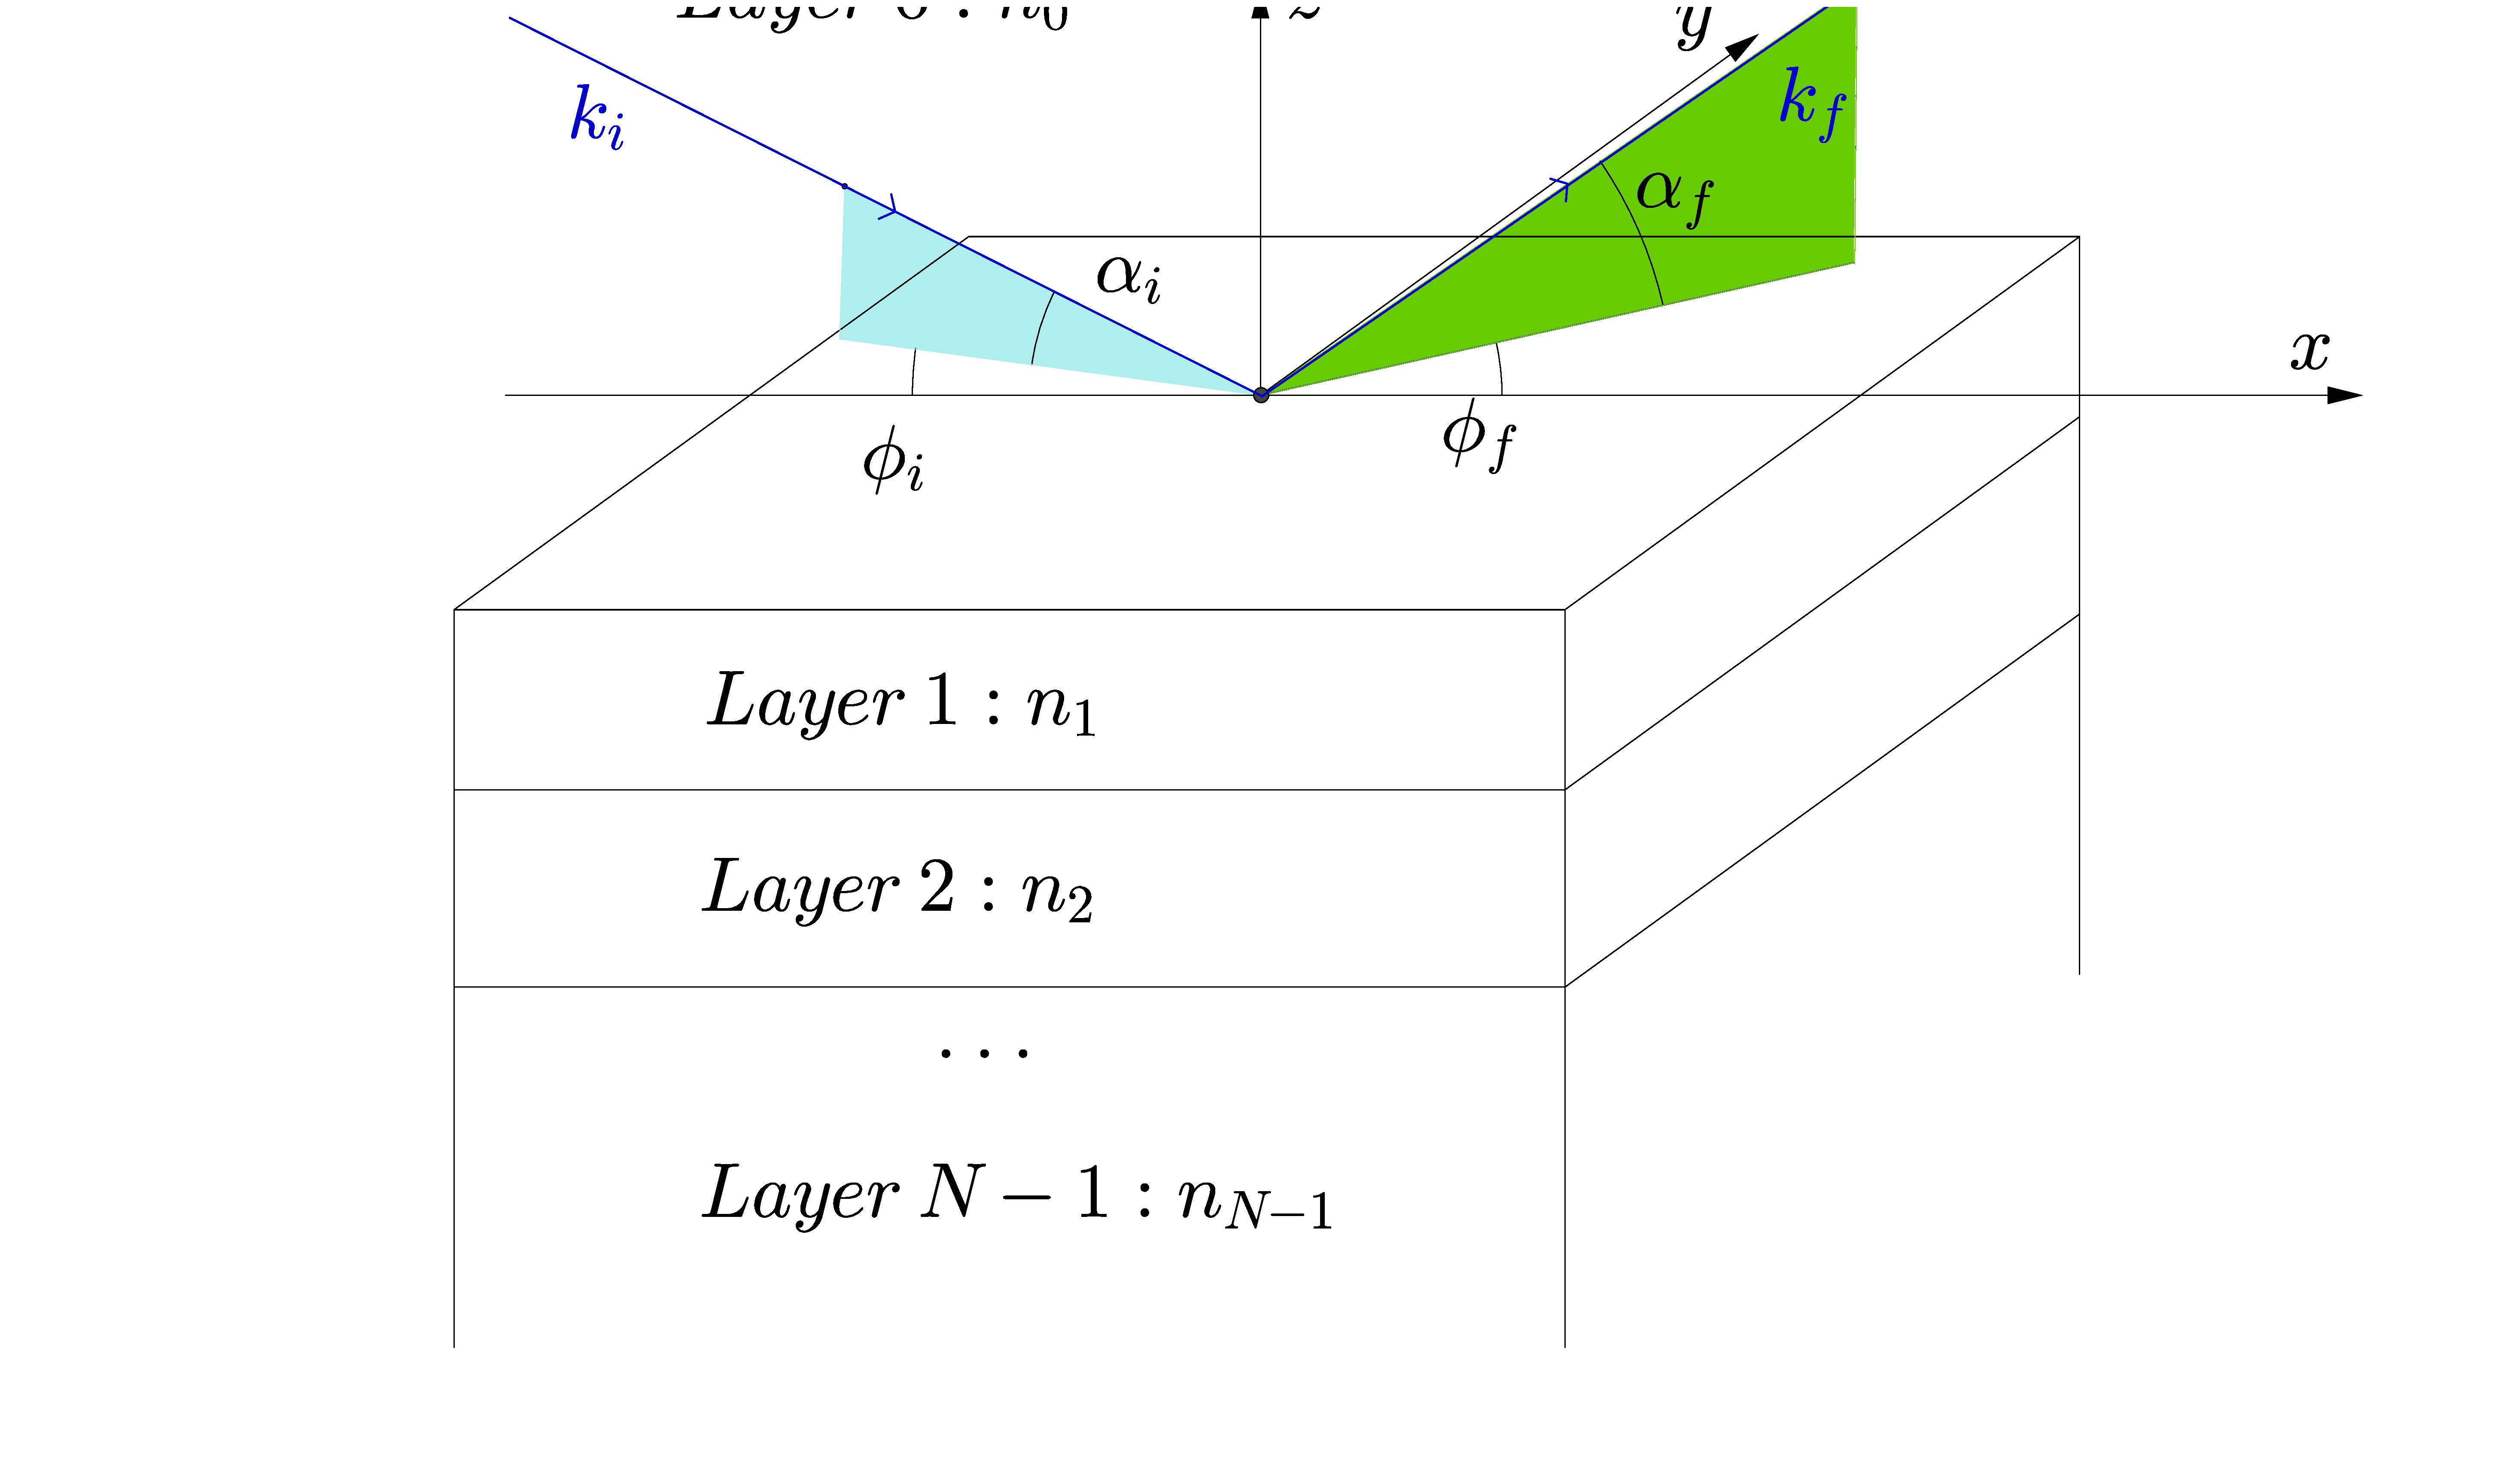
\includegraphics[clip=, width=120mm]{Figures/multilayer3d3.eps}
  \caption[Representation of the scattering geometry.]{Representation of the scattering geometry. $n_j$ is
    the refractive index of layer $j$ and $\alpha_i$ and $\phi_i$ are the incident
    angles of the wave propagating. $\alpha_f$ is the exit angle with respect to the sample's surface and
$\phi_f$ is the scattering angle with respect to the scattering
plane. }
  \label{fig:multil3d}
\end{figure}


\noindent The layers are defined by their thicknesses (parallel to the
$z$-direction), their possible
roughnesses (equal to 0 by default) and the
material they are made of. We do not define any dimensions in the $x$, $y$
directions. And, except for roughness, the layer's vertical boundaries are plane and
perpendicular to the $z$-axis. There is also no limitation to the
number of layers that could be defined in \BornAgain. Note that the
thickness of the top and bottom layer are not defined. \\

\ImportantPoint{Remark:}{Order of the different steps for the simulation: \\
When assembling the sample, the layers are defined from top to
bottom. So in most cases the first layer will be the air layer.}\\

\noindent The particles are characterized by their form factors (\textit{i.e.} the Fourier transform of the shape function - see the list of form factors implemented
  in \BornAgain) and the composing material. The number of input parameters for the form
  factor depends on the
  particle symmetry; it ranges from one parameter for a sphere (its
  radius) to three for an ellipsoid (its three main axis lengths).\\ By
  placing the particles
inside or on top of a layer, we impose their vertical positions, whose
values correspond to the bottoms of the particles. The in-plane distribution of particles is linked with the way the
particles interfere with each other. It is therefore implemented
when dealing with the interference function. \\

%\ImportantPoint{Remark:}{Depth of particles\\
%The vertical positions of particles in a layer are given in relative
%coordinates. For the top layer, the bottom corresponds to
%\texttt{depth}=0. But for all the other layers, it is the top of the
%layer which corresponds to \texttt{depth}=0.}\\

\noindent The complex refractive index associated with a layer or a particle is written as $n=1-\delta +i\beta$, with
$\delta, \beta \in \mathbb{R}$. In our program, we input $\delta$ and
$\beta$ directly.


\noindent The input beam is assumed to be monochromatic without any
spatial divergence.\\ %\textbf{polarization term?}

\subsection{Units}
By default the angles are expressed in radians and the lengths are given in
nanometers.  But it is possible to use other units by
specifying them right after the value of the corresponding
parameter like, for example, \Code{20.0*micrometer}.


\subsection{Programs}

The examples presented in the next paragraphs are written in \Python. For tutorials about this
   programming language, the users are referred to \cite{Lut09}.

%\noindent Note about the version of C++ and Python to run the examples.\\
%\noindent Where can the following examples be found?\\
%\noindent What is the command to run the examples?



%%%%%%%%%%%%%%%%%%%%%%%%%%%%%%%%%%%%%%%%%%%%%%%%%%%%%%%%%%%%%%%%%%%%%%%%%%%%%%%
%
%%%%%%%%%%%%%%%%%%%%%%%%%%%%%%%%%%%%%%%%%%%%%%%%%%%%%%%%%%%%%%%%%%%%%%%%%%%%%%%


%\mysection{Example 1}{Example 1: two types of islands on top of
%  substrate without interference.} \SecLabel{Example1Python}

\section{Example 1: two types of islands on top of
  substrate without interference.} \SecLabel{Example1Python}

% \sectionmark{Example 1}

In this example, we simulate the scattering from a mixture of
cylindrical and prismatic nanoparticles without any interference
between them. These particles are placed in air, on top
of a substrate.\\ We are going to go through each step of the
simulation. The Python script specific to each stage will be given at
the beginning of the description. But for the sake of completeness the full code is given
at the end of this section (Listing~\ref{script_ex1}). \\

\noindent We start by importing different functions from external
modules (line~\ref{import_lib}), for example NumPy, which
is a fundamental package for scientific computing with Python \cite{s:numpy}.  In particular, line~\ref{import_end}
imports the features of \BornAgain\ software.\\

\begin{lstlisting}[language=python, style=eclipseboxed,name=ex1,nolol]
import sys, os, numpy @\label{import_lib}@

from libBornAgainCore import * @\label{import_end}@
\end{lstlisting}


 %%%%%%%%%%%%%  
\myparagraph{\underline{First step:} Defining materials} 
 

\begin{lstlisting}[language=python, style=eclipseboxed,name=ex1,nolol]
def RunSimulation(): @\label{def_function}@
    #  defining materials @\label{material1}@
    mAmbience = MaterialManager.getHomogeneousMaterial("Air", 0.0, 0.0)  @\label{material2}@
    mSubstrate = MaterialManager.getHomogeneousMaterial("Substrate",
    6e-6, 2e-8) @\label{material3}@
    mParticle = MaterialManager.getHomogeneousMaterial("Particle", 6e-4,
  2e-8 ) @\label{materialparticle}@
\end{lstlisting}

\noindent Line~\ref{def_function} marks the beginning of the
function to define and run the simulation. 

\noindent Lines~\ref{material2}, \ref{material3} and \ref{materialparticle} define different
materials using function \Code{getHomogeneousMaterial} from class
\Code{MaterialManager}. The general syntax is the following 

\begin{lstlisting}[language=python, style=eclipse,numbers=none]
<material_name> = MaterialManager.getHomogeneousMaterial("name", delta, beta)
\end{lstlisting}

\noindent where \Code{name} is the name of the
material associated with its complex refractive index
n=1-\Code{delta} +i \Code{beta}. \Code{<material\_name>} is later used when
referring to this particular material. The three defined materials in this example are \Code{Air} with a refractive
index of 1 (\Code{delta = beta =0}), a \Code{Substrate} associated with a complex refractive index
equal to $1-6\times 10^{-6} +i2\times 10^{-8} $, and the material of particles, whose refractive index is \Code{n}$=1-6\times 10^{-4}+i2\times 10^{-8}$.\\\\

%\noindent \underline{Remark:} there is no condition on the choice of \Code{name}. 
 %%%%%%%%%%%%% 
\myparagraph{\underline{Second step:} Defining the particles} 

\begin{lstlisting}[language=python,style=eclipseboxed,name=ex1,nolol]
    # collection of particles @\label{particles1}@
    cylinder_ff = FormFactorCylinder(5*nanometer, 5*nanometer) @\label{particlescyl1}@
    cylinder = Particle(mParticle, cylinder_ff) @\label{particlescyl2}@
    prism_ff = FormFactorPrism3(5*nanometer, 5*nanometer) @\label{particlesprism1}@
    prism = Particle(mParticle, prism_ff) @\label{particlesprism2}@
\end{lstlisting}

 \noindent We implement two different shapes of particles: cylinders and
 prisms (\textit{i.e.} elongated particles with a constant equilateral triangular cross section).\\ All particles implemented in \BornAgain\ are defined by their
 form factors, their sizes and the material
  they are made of. Here, for the
  cylindrical particle, we input its radius and height.  For the prism, 
  the possible inputs are the length of one side of its equilateral triangular
  base and its height.\\

%\noindent In line~\ref{complx_ref_index}, we define the complex refractive index
%associated with both particle shapes: \Code{n}$=1-6\times 10^{-4}+i2\times 10^{-8}$.\\
  
\noindent In order to define a particle, we proceed in two steps. For example for
the cylindrical particle, we first specify the form factor of a cylinder with 
its radius and height, both equal to 5 nanometers in this particular
case (see line~\ref{particlescyl1}). Then we associate this shape with
the constituting material as in line~\ref{particlescyl2}.\\

\noindent The same procedure has been applied for the prism in lines~\ref{particlesprism1} and \ref{particlesprism2} respectively.
 %%%%%%%%%%%%% 
\myparagraph{\underline{Third step:} Characterizing the layers and assembling the sample} 

\noindent \textbf{Particle decoration} \\
  

\begin{lstlisting}[language=python, style=eclipseboxed, name=ex1,nolol]
    particle_decoration = ParticleDecoration()  @\label{particlesdecor1}@
    particle_decoration.addParticle(cylinder, 0.0, 0.5)  @\label{particlesdecor2}@
    particle_decoration.addParticle(prism, 0.0, 0.5)@\label{particlesdecor3}@
    interference = InterferenceFunctionNone()  @\label{particlesnointerf}@
    particle_decoration.addInterferenceFunction(interference)  @\label{particlesinterf}@
\end{lstlisting}

\noindent The object which holds the information about the positions and densities of particles
in our sample is called \Code{ParticleDecoration}
(line~\ref{particlesdecor1}). We use the associated function \Code{addParticle}
for each particle shape (lines~\ref{particlesdecor2}, \ref{particlesdecor3}). Its general
syntax is 

\begin{lstlisting}[language=python, style=eclipse,numbers=none]
addParticle(<particle_name>, depth, abundance) 
\end{lstlisting}

\noindent  where \Code{<particle\_name>} is the name used to define the particles
(lines~\ref{particlescyl2} and \ref{particlesprism2}), \Code{depth}
(default value =0)
is the vertical position, expressed in nanometers, of the particles in a given layer (the
association with a particular layer will be done during the next step) and
\Code{abundance} is the proportion of this type of particles, 
normalized to the total number of particles. Here we have 50\% of cylinders
and 50\% of prisms. \\ 

\ImportantPoint{Remark:}{Depth of particles\\
The vertical positions of particles in a layer are given in relative
coordinates. For the top layer, the bottom corresponds to
\Code{depth}=0 and negative values would correspond to particles
floating above layer 1 since the vertical axis, shown in \reffig{multil3d} is pointing upwards. But for all the other layers, it is the top of the
layer which corresponds to \Code{depth}=0.}\\


\noindent Finally lines~\ref{particlesnointerf} and
\ref{particlesinterf} specify that there is \textbf{no coherent interference} between
the waves scattered by these particles. The intensity is calculated by
the incoherent sum of the scattered waves: $\langle |F_n|^2\rangle$,
where $F_n$ is the form factor associated with the particle of type $n$.  The way these waves
interfere imposes the horizontal distribution of
the particles as
the interference reflects the long or short-range order of the
particles distribution (\textbf{see Theory}). On the contrary, the vertical position is
imposed when we add the particles in a given layer by parameter \Code{depth}, as shown in lines~\ref{particlesdecor2} and \ref{particlesdecor3}. \\

\noindent \textbf{Multilayer}\\
  
\begin{lstlisting}[language=python, style=eclipseboxed,name=ex1,nolol]
    # air layer with particles and substrate form multi layer  @\label{sampleassembling}@
    air_layer = Layer(mAmbience)  @\label{airlayer}@
    air_layer.setDecoration(particle_decoration)  @\label{airlayerdecorator}@
    substrate_layer = Layer(mSubstrate, 0)  @\label{substratelayer}@
    multi_layer = MultiLayer()  @\label{multilayercanvas}@
    multi_layer.addLayer(air_layer)  @\label{layerairdecor}@
    multi_layer.addLayer(substrate_layer)  @\label{layersubstrate}@
\end{lstlisting}

\noindent We now have to configure our sample. For this first example,
the particles, \textit{i.e.} cylinders and prisms, are on top of a substrate in an
air layer. \textbf{The order in which we define these layers is important: we
start from the top layer down to the bottom one}.\\

\noindent Let us start with the air layer. It contains the particles. In
line~\ref{airlayer}, we use the previously defined \Code{mAmbience}
(="air" material) (line~\ref{material2}). The command written in line~\ref{airlayerdecorator} shows that this layer is decorated by adding the
particles using the function \Code{particle\_decoration} defined in
lines~\ref{particlesdecor1}-\ref{particlesinterf}. The substrate layer
only contains the substrate material (line~\ref{substratelayer}).\\%Note that the
%\Code{depth} is referenced to the bottom of the top layer (negative
%values would correspond to particles floating above layer 1 as
%the vertical axis is pointing upwards). 
 
\noindent There are different possible syntaxes to define a layer. As shown in
lines~\ref{airlayer} and \ref{substratelayer}, we can use
\Code{Layer(<material\_name>,thickness)} or
\Code{Layer(<material\_name>)}. The second case corresponds
to the default value of the \Code{thickness}, equal to 0. The \Code{thickness} is
expressed in  nanometers. \\

\noindent Our two layers are now fully characterized. The sample is assembled using
\Code{MultiLayer()} constructor (line~\ref{multilayercanvas}): we start with the air layer decorated
with the particles (line~\ref{layerairdecor}), which is the layer at
the top and end with the bottom layer, which is the
substrate (line~\ref{layersubstrate}).
 %%%%%%%%%%%%% 
\myparagraph{\underline{Fourth step:} Characterizing the input beam and
output detector and running the simulation} 


\begin{lstlisting}[language=python, style=eclipseboxed,name=ex1,nolol]
    # run simulation  @\label{run1}@
    simulation = Simulation()  @\label{run2}@
    simulation.setDetectorParameters(100,-1.0*degree, 1.0*degree, 
                                100, 0.0*degree, 2.0*degree, True)  @\label{rundetector}@
    simulation.setBeamParameters(1.0*angstrom, 0.2*degree, 0.0*degree)  @\label{runbeam}@
    simulation.setSample(multi_layer)  @\label{runsample}@
    simulation.runSimulation()  @\label{runsimul}@
\end{lstlisting}


\noindent The first stage is to define the \Code{Simulation()} object (line~\ref{run2}). Then we define the detector (line~\ref{rundetector}) and beam
parameters (line~\ref{runbeam}), which are associated with the
sample previously defined (line~\ref{runsample}). Finally we run
the simulation (line~\ref{runsimul}). Those functions are part of the Simulation
class.  The
different incident and exit angles are
shown in \reffig{multil3d}. \\

\noindent The detector parameters are set using ranges of angles via
the function:\\

\noindent \Code{setDetectorParameters(n\_phi, phi\_f\_min,
  phi\_f\_max,\\ \phantom{setDetectorParameters(}n\_alpha, alpha\_f\_min, alpha\_f\_max, isgisaxs\_style=false)}, \\

\noindent where \Code{n\_phi=100} is the number of iterations for $\phi_f$,\\ \Code{phi\_f\_min=-1.0*degree} and \Code{phi\_f\_max=1.0*degree}
are the minimum and maximum values respectively of $\phi_f$, \\ \Code{n\_alpha=100} is
the number of iterations for $\alpha_f$,\\ \Code{alpha\_f\_min=0.0*degree} and \Code{alpha\_f\_max=2.0*degree} 
are the minimum and maximum values respectively of
$\alpha_f$. \\
\Code{isgisaxs\_style=True} (default value = \Code{False}) is a boolean
used to characterise the structure of the output data. If
\Code{isgisaxs\_style=True}, the output data is binned at constant
values of the sine of the output angles, $\alpha_f$ and $\phi_f$, otherwise it is binned
at constant values of these two angles.\\


\noindent For the beam the function to use is
\Code{setBeamParameters(lambda, alpha\_i, phi\_i)}, where\\
\Code{lambda=1.0*angstrom} is the incident beam wavelength,
\Code{alpha\_i=0.2*degree} is the incident
grazing angle on the surface of the sample,
\Code{phi\_i=0.0*degree} is the in-plane
direction of the incident beam (measured with respect to the
$x$-axis).\\ 

\noindent \underline{Remark}: Note that, except for
\Code{isgisaxs\_style}, there are no default values implemented for the
parameters of the beam and detector.\\

\noindent Line~\ref{runsimul} shows the command to run the simulation using the
previously defined setup.
%%%%%%%%%%%%%
\myparagraph{\underline{Fifth step:} Saving the data} 


\begin{lstlisting}[language=python, style=eclipseboxed,name=ex1,nolol]
    # retrieving intensity data
    return GetOutputData(simulation) @\label{outputdata}@
\end{lstlisting}


\noindent In line~\ref{outputdata} we obtain the simulated intensity
as a function of outgoing angles $\alpha_f$ and $\phi_f$ for further
uses (plots, fits,\ldots) as a NumPy array containing
\Code{n\_phi}$\times$\Code{n\_alpha}
datapoints. Some options are provided by \BornAgain. For example, \reffig{output_ex1} shows the two-dimensional
contourplot of the intensity as a function of $\alpha_f$ and
$\phi_f$. 

\begin{figure}[p!]
  \begin{center}
   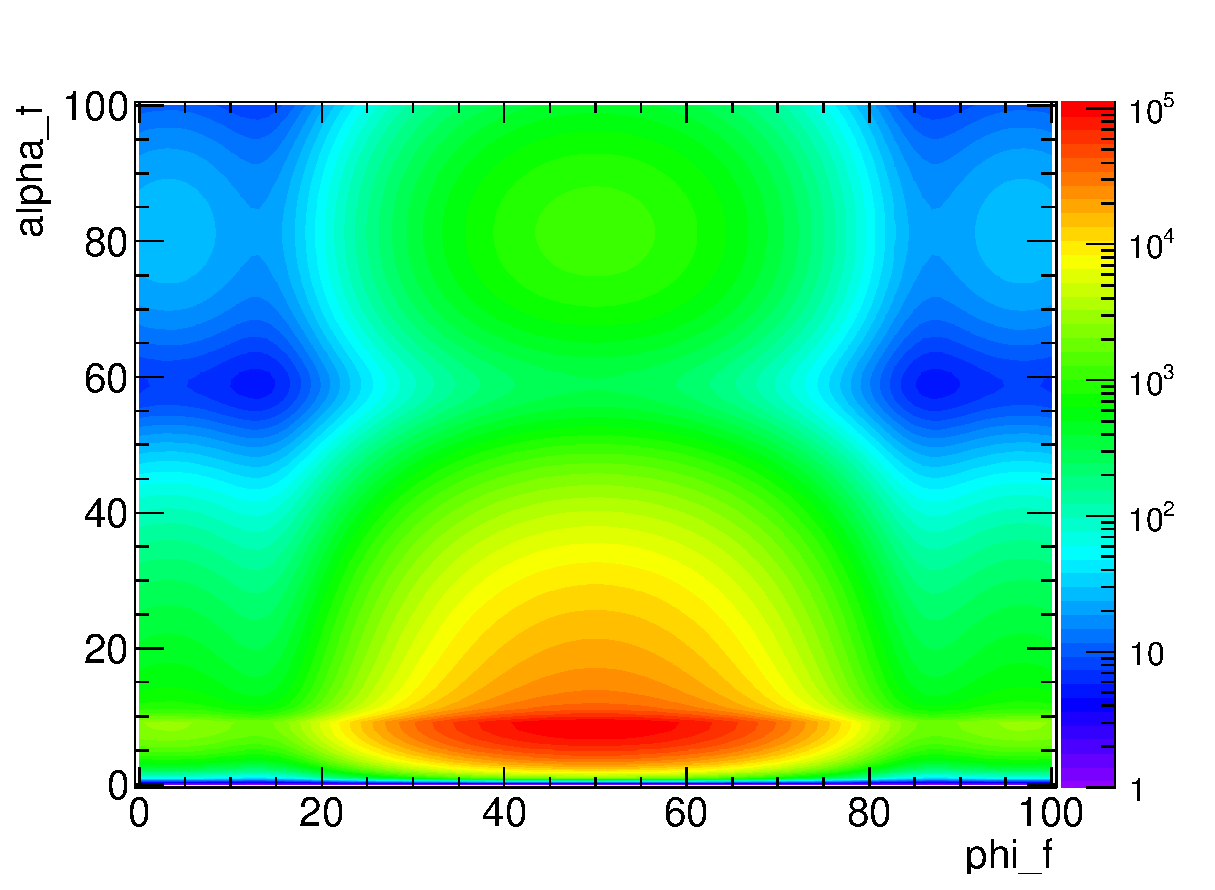
\includegraphics[clip=true, width=120mm]{Figures/Manual_ex1.eps}
  \end{center}
  \caption[Example 1: Simulated grazing-incidence small-angle X-ray scattering from a mixture of
cylindrical and prismatic nanoparticles without any interference, deposited on top
of a substrate]{Figure of example 1: Simulated grazing-incidence small-angle X-ray scattering from a mixture of
cylindrical and prismatic nanoparticles without any interference, deposited on top
of a substrate. The input beam is characterized by a wavelength
$\lambda$ of 1~\AA\ and incident angles $\alpha_i=0.2^{\circ}$, $\phi_i=0^{\circ}$. The
cylinders have a radius and a height both equal to 5~nm, the prisms
are characterized by a side length equal to 5~nm and they are also 5~nm high. The
material of the particles has a refractive index of $1-6\times 10^{-4}+i2\times 10^{-8}$. For the substrate
it is equal to $1-6\times 10^{-6} +i2\times 10^{-8} $. The colorscale
is associated with the output intensity in arbitrary units. }
\label{fig:output_ex1}
\end{figure}



%%%%%%%%%%%%%%%%%%%%%%%%%%%%%%%%%%%%%%%%%%%%%%%%%%%%%%%%%%%%%%%%%%%%%%%%%%%%%%%
%
%%%%%%%%%%%%%%%%%%%%%%%%%%%%%%%%%%%%%%%%%%%%%%%%%%%%%%%%%%%%%%%%%%%%%%%%%%%%%%%
\section{Example 2: working with sample parameters.} \SecLabel{WorkingWithSampleParameters}

This section gives additional details about the manipulation of sample parameters
at run time, that is after the sample has already been constructed. 
For single simulation this is normally not necessary, however it might be useful
during interactive work when user tries to find optimal sample parameters by
running a series of consequent simulations.
Similarly, this task arises when the theoretical model, presented by the sample and the simulation descriptions, is used for the fitting of real data.
In this case fitting kernel has to be informed about existing sample parameters
and has to have a mechanism for changing values of these parameters to find 
they optimal values.

In \BornAgain\ this is done using so called sample parameter pool mechanism 
and we will briefly explain it using example from the previous
\SecRef{Example1Python}.

Inside \BornAgain\ sample is described by a hierarchical tree of objects.
For the multilayer created in previous section this tree can be graphically
represented as shown in Fig.~\ref{fig:sample_tree}. 

\begin{figure}[p!]

\tikzstyle{every node}=[draw=black,thick,anchor=west]
\tikzstyle{selected}=[draw=red,fill=red!30]
\tikzstyle{optional}=[dashed,fill=gray!50]
\begin{tikzpicture}[%
  grow via three points={one child at (0.5,-0.7) and
  two children at (0.5,-0.7) and (0.5,-1.4)},
  edge from parent path={(\tikzparentnode.south) |- (\tikzchildnode.west)}]
  \node {MultiLayer}
    child { node {Layer \#0}
		child { node {ParticleDecoration } 
			child { node {Particle Info 0} 
				child {node {Particle }  
					child { node {FormFactorCylinder} 
						child { node [optional] { height:5.0} }					
						child { node [optional] { radius:5.0} }					
					}				
				}
    			child [missing] {}		
    			child [missing] {}		
			    child [missing] {}		
				child {node [optional] { abundance:0.5} }			
				child {node [optional] { depth:0.0} }			
			}
    		child [missing] {}		
    		child [missing] {}		
			child [missing] {}		
    		child [missing] {}		
    		child [missing] {}		
			child [missing] {}		
			child { node {Particle Info 1} 
				child {node {Particle }  
					child { node {FormFactorPrism3} 
						child { node [optional] { half\_side:5.0} }					
						child { node [optional] { height:5.0} }					
					}				
				}
    			child [missing] {}		
    			child [missing] {}		
			    child [missing] {}		
				child {node [optional] { abundance:0.5} }			
				child {node [optional] { depth:0.0} }						
			}					
		}
		child [missing] {}		
   		child [missing] {}		
	    child [missing] {}		
		child [missing] {}		
   		child [missing] {}		
	    child [missing] {}		
	    child [missing] {}		
		child [missing] {}		
   		child [missing] {}		
	    child [missing] {}		
		child [missing] {}		
   		child [missing] {}		
	    child [missing] {}		
	    child [missing] {}		
		child {node [optional] { thickness:0.0} }				
    }
	child [missing] {}		
   	child [missing] {}		
	child [missing] {}		
   	child [missing] {}		
	child [missing] {}		
	child [missing] {}		
   	child [missing] {}		
	child [missing] {}		
   	child [missing] {}		
	child [missing] {}		
	child [missing] {}		
   	child [missing] {}		
	child [missing] {}		
   	child [missing] {}		
	child [missing] {}		
	child [missing] {}		
	child { node {Layer interface \#0} 
    	child {node { roughness} 
    		child {node [optional] { corrlength:0.0} }				    	
    		child {node [optional] { hurst:0.0} }				    	
    		child {node [optional] { sigma:0.0} }				    	
    	}					
	}
   	child [missing] {}		
	child [missing] {}		
	child [missing] {}		
    child { node {Layer \#1}
    	child {node [optional] { thickness:0.0} }				
    }
	child [missing] {}		
    child { node [optional] {CrossCorrLength:0.0} };
    
\end{tikzpicture}
\caption{Tree representation of the sample structure.}
\label{fig:sample_tree}
\end{figure}


The top \Code{MultiLayer} object is composed of three children, namely
\Code{Layer \#0, Layer Interface \#0} and \Code{Layer \#1}. Children objects
by turn might also be composed into tree-like structure. For example,
\Code{Layer \#0} contains \Code{ParticleDecoration} object which holds all information
related to the particles populating the layer. All numerical values which have been used
during sample construction (thickness of layers, size of particles, roughness parameters) are the part of the same tree structure. 
They are marked in the figure with shaded gray boxes.

These values are registered in the sample parameter pool using the name
composed from the names of corresponding nodes of the tree and can be accessed/changed
during run time. For example, the \Code{height} of the cylinders populating first layer can be changed from 
current $5~nm$ to $1~nm$ by running the command

\begin{lstlisting}[language=shell, style=commandline]
multi_layer.setParameterValue('/MultiLayer/Layer0/ParticleDecoration/ParticleInfo0/Particle/FormFactorCylinder/height', 1.0)
\end{lstlisting}


The user can get names and values of all registered sample's parameters using the command 

\begin{lstlisting}[language=shell, style=commandline]
> multi_layer.printParameters()
The sample contains following parameters ('name':value)
'/MultiLayer/Layer0/ParticleDecoration/ParticleInfo0/Particle/FormFactorCylinder/height':5
'/MultiLayer/Layer0/ParticleDecoration/ParticleInfo0/Particle/FormFactorCylinder/radius':5
'/MultiLayer/Layer0/ParticleDecoration/ParticleInfo0/abundance':0.5
'/MultiLayer/Layer0/ParticleDecoration/ParticleInfo0/depth':0
'/MultiLayer/Layer0/ParticleDecoration/ParticleInfo1/Particle/FormFactorPrism3/half_side':5
'/MultiLayer/Layer0/ParticleDecoration/ParticleInfo1/Particle/FormFactorPrism3/height':5
'/MultiLayer/Layer0/ParticleDecoration/ParticleInfo1/abundance':0.5
'/MultiLayer/Layer0/ParticleDecoration/ParticleInfo1/depth':0
'/MultiLayer/Layer0/thickness':0
'/MultiLayer/Layer1/thickness':0
'/MultiLayer/LayerInterface/roughness/corrlength':0
'/MultiLayer/LayerInterface/roughness/hurst':0
'/MultiLayer/LayerInterface/roughness/sigma':0
'/MultiLayer/crossCorrLength':0
\end{lstlisting}

Wildcards \Code{'*'} can be used to reduce typing or to work on group of parameters. In example below first command will change the height of the cylinders in the same way, as in previous example, while the second line will change the depth of both cylinders and prisms.
\begin{lstlisting}[language=shell, style=commandline]
multi_layer.setParameterValue('*FormFactorCylinder/height', 1.0)
multi_layer.setParameterValue('*depth', 1.0)
\end{lstlisting}

The complete example to this section can be found at
\begin{lstlisting}[language=shell, style=commandline]
./Examples/python/fitting/ex001_SampleParametersIntro.py
\end{lstlisting}









\chapter{Scattering cross--section}  \SecLabel{ScatteringCrosssection}

%%%%%%%%%%%%%%%%%%%%%%%%%%%%%%%%%%%%%%%%%%%%%%%%%%%%%%%%%%%%%%%%%%%%%%%%%%%%%%%%
\section{Position of the problem} 
%%%%%%%%%%%%%%%%%%%%%%%%%%%%%%%%%%%%%%%%%%%%%%%%%%%%%%%%%%%%%%%%%%%%%%%%%%%%%%%%

This section describes how assemblies of particles and layers of materials contribute to the scattering cross--section \textit{i.e.} the way their spatial distributions, the distribution of shapes and their correlations or the layers' roughness can influence the output intensity. 

The samples generated with \BornAgain\ are made of different layers of materials characterized by their thicknesses, refractive indices, and possible surface roughnesses. Except for the thickness, the other dimensions of the layers are infinite.\\ Particles can be embedded in or deposited on the top of any layers. Those particles are characterized by their shapes, refractive indices, their spatial distribution and concentration in the sample. The influence of the particles' shapes is described by the form factors. When the particles are densely packed, the distance relative to each other becomes of the same order as the particles' sizes. The radiation scattered from these various particles are going to interfere together. \\ We are first going to give a short overview of the theory involved, mostly in order to define the terminology. For a more complete theoretical description, the user is referred to, for example, reference~\cite{ReLL09} and appendix \ref{appendixtheory} of this manual. Then we are going to describe how the interference features, the form factors and the characteristics of the material layers have been implemented in \BornAgain\ and  give some examples.


%%%%%%%%%%%%%%%%%%%%%%%%%%%%%%%%%%%%%%%%%%%%%%%%%%%%%%%%%%%%%%%%%%%%%%%%%%%%%%%%
\section{Collection of particles} \SecLabel{sect:interf}
%%%%%%%%%%%%%%%%%%%%%%%%%%%%%%%%%%%%%%%%%%%%%%%%%%%%%%%%%%%%%%%%%%%%%%%%%%%%%%%%

Let us consider the general geometry of a scattering experiment. An incident neutron with a wave vector $\mathbf{k}_i$ is scattered in a new direction $\mathbf{k}_f$ after interacting with a particle. This scattering occurs in a cone of solid angle $d\Omega$ around the direction of the scattered wave vector $\mathbf{k}_f$.
Considering a set of $N$ particles labeled with index $i$, located at $\mathbf{R}_i$ and having shapes $S_i(\mathbf{r})$ ($S_i=0$ outside the particle and 1 inside), occupying a total volume $V$, the differential cross--section per particle is given by:
\begin{equation*}
  \frac{d\sigma}{d\Omega}(\vect{q}) = \frac{1}{N}\left\lbrace \sum_i \left\lvert F_i(\vect{q}) \right\rvert ^2 + \sum_{i\neq j} F_i(\vect{q}) F_{j}^*(\vect{q}) \exp \left[i\vect{q}\cdot (\vect{R}_i-\vect{R}_j)\right] \right\rbrace \; .
\end{equation*}
where  $\mathbf{q}=\mathbf{k}_i - \mathbf{k}_f$ is the wave vector transfer and $F_i$ is the form factor of particle $i$ (see \SecRef{sect:ff} for a description).


Since in most experimental conditions only the statistical properties of the particles are known, one can consider the probabilistic value of this cross--section \textit{i.e.} its expectation value. Assuming that the particles' shapes are determined by their class $\alpha$, with the abundance ratio $p_\alpha \equiv N_\alpha / N$, and defining the particle density as $\rho_V \equiv N/V$, the expectation value becomes:
\begin{align*}
  \left\langle \frac{d\sigma}{d\Omega}(\vect{q}) \right\rangle  & = \sum_\alpha p_\alpha \left\lvert F_\alpha(\vect{q})\right\rvert ^2 + \frac{\rho_V}{V}\sum_{\alpha,\beta} p_\alpha p_\beta F_\alpha (\vect{q})F_\beta^*(\vect{q})  \\
  & \times \iint_V d^3\vect{R}_\alpha d^3\vect{R}_\beta \ppcf{\alpha}{\beta}{R} \exp \left[ i\vect{q}\cdot (\vect{R}_\alpha - \vect{R}_\beta ) \right] \; ,
\end{align*}

where $\ppcf{\alpha}{\beta}{R}$ is called the \emph{partial pair correlation function}. It represents the normalized probability of finding particles of type $\alpha$ and $\beta$ in positions $\vect{R}_\alpha$ and $\vect{R}_\beta$ respectively. 

%%%%%%%%%%%%%%%%%%%%%%%%%%%%%%%%%%%%%%%%
\subsection{Size-distribution models}

To proceed further, when the morphology and topology are not exactly known, some hypotheses need to be made since the correlation between the kinds of scatterers and their relative positions included in the pair correlation functions are difficult to estimate. Several options are available:

\paragraph{Decoupling approximation (DA)} neglects all correlations. It supposes that the particles are positioned in a way that is completely independent on their kinds (shapes, sizes). An example is given in figure~\ref{fig:da}. Thus the kind of scattering objects and their positions are not correlated and the partial pair correlation function is independent of the particle class $\alpha$. We can therefore replace $ \ppcfb{\alpha}{\beta}{R}$ by  $g(\vect{R}_{\alpha\beta})$.

This leads to the following expression of the scattering cross--section:
\begin{equation*}
\left\langle \frac{d\sigma}{d\Omega}(\vect{q}) \right\rangle  = I_d(\vect{q}) + \left\lvert \left\langle F_\alpha(\vect{q}) \right\rangle_\alpha \right\rvert ^2 \times S(\vect{q}) \; ,
\end{equation*}
where $I_d$ is the diffuse part of the scattering. It is the signature of the fluctuations of shapes, sizes or orientations of the particles; its maximum is located in $q_{\parallel}=0$. In the second term of the expression of the scattering cross-section, $S(\vect{q})$ is the interference function and is given by
\begin{equation*} 
  S(\vect{q}) = 1+ \rho_V \int_V d^3\vect{R} \; g(\vect{R}) \exp \left[ i\vect{q}\cdot \vect{R} \right] \; .
\end{equation*}


\begin{figure}[ht]
\begin{center}
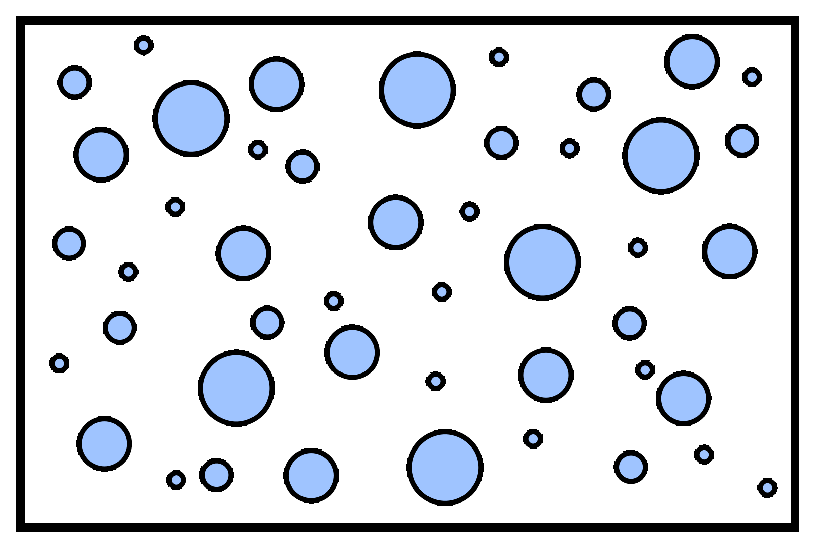
\includegraphics[width=0.5\textwidth]{Figures/drawing/drawingDA.eps}
\end{center}
\caption{Sketch of a collection of particles deposited on a substrate whose scattering  could be described by the decoupling approximation.}
\label{fig:da}
\end{figure}


In concentrated systems, DA breaks down because of correlations. One solution is to reintroduce some correlations between particles sizes and distributions using, for example, the size spacing correlation approximation described below. 

\paragraph{Local monodisperse approximation (LMA)} partially accounts for some coupling between the positions and the kinds of the particles \cite{Ped94}. 
 It requires a subdivision of the layers of particles into monodisperse domains. The contributions of these subdomains are then  incoherently summed up and weighted by the size-shape probabilities.\\ In this approximation, a particle is supposed to be surrounded by particles of the same size and shape, within the coherence length of the input beam (see fig.~\ref{fig:lma}). The scattering cross--section is expressed as
\begin{equation*}
  \left\langle \frac{d\sigma}{d\Omega}(\vect{q}) \right\rangle \simeq \left\langle \left\lvert F_\alpha(\vect{q})\right\rvert ^2 S_\alpha(\vect{q}) \right\rangle_\alpha \; .
\end{equation*}

Contrary to the Decoupling Approximation, the Local Monodisperse Approximation can account for particle class/size/shape--dependent pair correlation functions by having distinct interference functions $S_\alpha(\vect{q})$.

One has to remember that in most cases, this approximation corresponds to an unphysical description of the investigated systems. \\ 

DA and LMA separate the contributions of the form factors and of the interference function. For disordered systems DA and LMA give the same result as the scattering vector gets larger \textit{i.e.} the scattered intensity is dominated by the contribution of the form factor.

\begin{figure}[ht]
\begin{center}
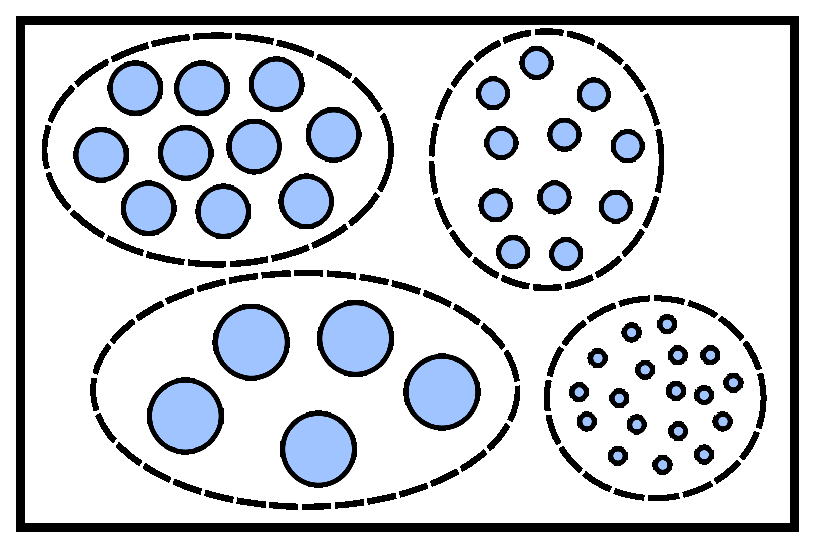
\includegraphics[width=0.5\textwidth]{Figures/drawing/drawingLMA.eps}
\end{center}
\caption{Sketch of a collection of particles deposited on a substrate whose scattering could be described by the local monodisperse correlation approximation. The dashed areas mark the coherent domains. In this case, the total scattering intensity is the incoherent sum from all these domains.}
\label{fig:lma}
\end{figure}

\paragraph{Size spacing correlation approximation (SSCA)} introduces correlations between polydisperse particles, more precisely between the size of the particles and their mutual spacing. A classical example would consist in particles whose closest--neighbour spacing depends linearly on the sum of their respective sizes \cite{LaLR07}, as illustrated in fig.~\ref{fig:ssca}.

%For a sample where only the statistical properties of particle positions and size are known, the scattered intensity per scattering particle is expressed as the average over an ensemble of the Fourier transform of the Patterson function, which is the autocorrelation of the scattering length density $\curlp (\vectr ) \equiv \sum_{ij} S_i(-\vectr )\otimes S_j(\vectr )\otimes \delta (\vectr + \vectr_i - \vectr_j )$:
%\begin{equation*}
%  I(\vectq ) = \frac{1}{N}\ensavg{}{\curlf (\curlp (\vectr ))} \; ,
%\end{equation*}
%where $\curlf$ denotes the Fourier transform and $\curlp$ the Patterson function

\begin{figure}[ht]
\begin{center}
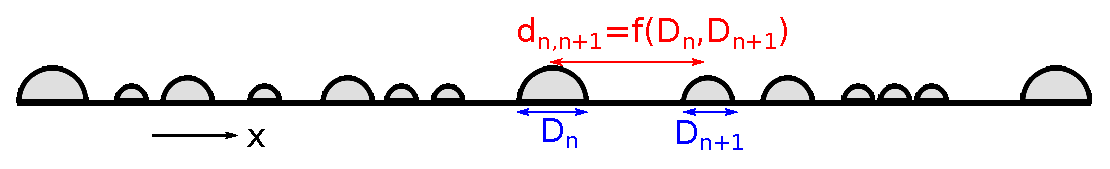
\includegraphics[width=0.9\textwidth]{Figures/drawing/drawingSSCA.eps}
\end{center}
\caption{Sketch of a 1D distributed collection of particles, whose scattering could be described by the size-spacing correlation approximation: the distance between two particles depends on their sizes.}
\label{fig:ssca}
\end{figure}



\MakeRemark{Terminology}{
\\
For collections of particles, the scattered intensity contains contributions from neighboring particles. This additional pattern can be called the structure factor, the interference function or even in crystallography, the lattice factor. In this manual, we use the term "interference function" or interferences.
}

%%%%%%%%%%%%%%%%%%%%%%%%%%%%%%%%%%%%%%%%
\subsection{Layout of particles}\label{sec:partlayout}

\subsubsection{The uncorrelated or disordered lattice}
For very diluted distributions of particles, the particles are too far apart from each other to lead to any interference between the waves scattered by each of them. In this case the interference function is equal to 1. The scattered intensity is then entirely determined by the form factors of the particles distributed in the sample.

\subsubsection{The regular  lattice}\mbox{}\\
The particles are positioned at regular intervals generating a layout characterised by its base vectors $\mathbf{a}$ and $\mathbf{b}$ (in direct space) and the angle between these two vectors.
This lattice can be two or one-dimensional depending on the characteristics of the particles. For example when they are infinitely long, the implementation can be simplified and reduced to a "pseudo" 1D system.

\paragraph{The ideal paracrystal} \mbox{}\\
A paracrystal, whose notion  was developed by Hosemann\cite{Hos51}, allows fluctuations of the lengths and orientations of lattice vectors. Paracrystals can be defined as distorted crystals in which the crystalline order has not disappeared and for which the behavior of the interference functions  at small angles is coherent.
It is a transition between the regular lattice and the disordered state.\\


For example, in one dimension, a paracrystal is generated using the following method. First we place a particle at the origin. The second particle is put at a distance $x$ with a density probability $p(x)$ that is peaked at a mean value $D$: $\int_{-\infty} ^{\infty}p(x)dx=1$ and $\int_{-\infty}^{\infty}xp(x)dx=D$. The third one is added at a distance $y$ from the second site using the same rule with a density probability $p_2(y)= \int_{-\infty}^{\infty}p(x)p(y-x)dx=p\otimes p(y)$.\\ With such a method, the pair correlation function $g(x)$ is built step by step. Its expression and the one of its Fourier transform, which is the interference function are 
\begin{equation*}
g(x)=\delta(x)+ p(x)+ p(x)\otimes p(x)+\ldots + p(-x)+\ldots \: \mathrm{and}\:\, S(q)=\Re\left(\dfrac{1+P(q)}{1-P(q)}\right),
\end{equation*}
 where $P(q)$ is the Fourier transform of the density probability $p(x)$.\\

\paragraph{Example} For a probability distribution function is Gaussian:
\begin{equation*}
p(x)=\frac{1}{\omega \sqrt{2\pi}} \exp\left(-\dfrac{(x-D)^2}{\omega^2}\right),\qquad P(q)=\exp\left(-\frac{q^2 \omega^2}{2}\right)\exp(iqD).
\end{equation*}
 The interference function of a one-dimensional paracrystal is given by

\begin{align*}
S(q) =\Re \left(\frac{1+\Phi(q) }{1 - \Phi(q)} \right), \quad \mathrm{where}\quad \Phi(q) = P(q)\exp\left(-\frac{D}{\Lambda}\right),
\end{align*}
where $\Lambda$ is a damping length used in order to introduce some finite-size effects.

Figure~\ref{fig:1dparas_q} shows the evolution of $S(q)$ for different values of $\omega /D$. 

\begin{figure}[ht]
\begin{center}
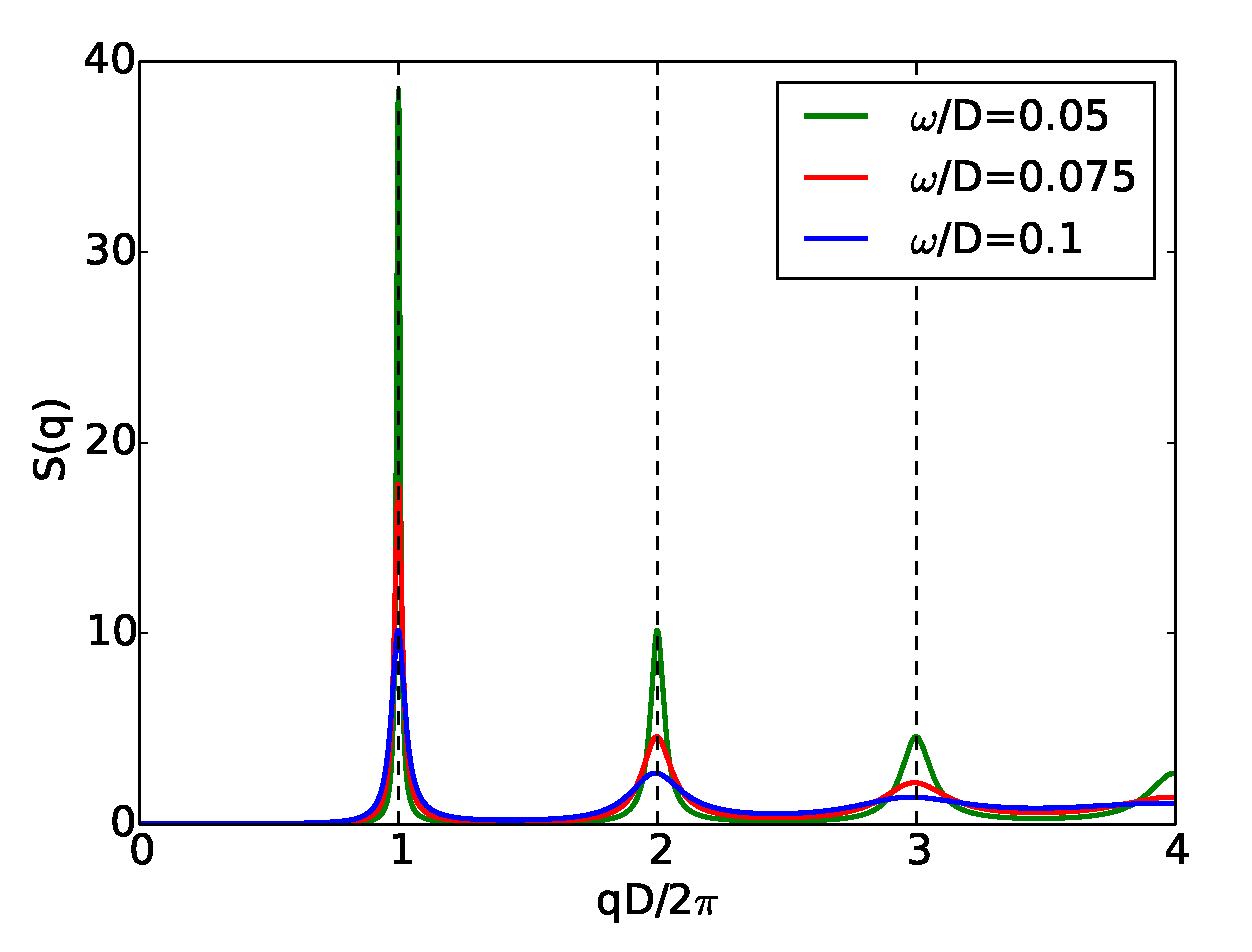
\includegraphics[width=0.6\textwidth]{Figures/funcplot/S_q_1Dparacrystal.eps}
\end{center}
\caption{Interference function of a 1D Gaussian paracrystal plotted for different values of $\omega /D$. The peaks broaden with a decreasing amplitude as $\omega/D$ increases. This shows the transition between an ordered and a disordered states. }
\label{fig:1dparas_q}
\end{figure}



In two dimensions, the paracrystal is constructed on a pseudo-regular lattice with base vectors $\mathbf{a}$ and $\mathbf{b}$ using the following conditions for the densities of probabilities:\\ $\int p_{\mathbf{a}}(\mathbf{r})d^2\mathbf{r}=\int p_{\mathbf{b}}(\mathbf{r})d^2\mathbf{r}=1$, $\int \mathbf{r} p_{\mathbf{a}}(\mathbf{r})d^2\mathbf{r}=\mathbf{a}$, $\int \mathbf{r} p_{\mathbf{b}}(\mathbf{r})d^2\mathbf{r}=\mathbf{b}$.\\
In the ideal case the deformations along the two axes are decoupled and each unit cell should retain a parallelogram shape. The interference function is given by\\ $S(q_{\parallel})=\prod_{k=a,b}\Re\left(\dfrac{1+P_k(q_{\parallel})}{1-P_k(q_{\parallel})} \right)$ with $P_k$ the Fourier transform of $p_k$, $k=a, b$.

\paragraph{Probability distributions} \mbox{}\\
The scattering by an ordered lattice gives rise to a series of Bragg peaks situated at the nodes of the reciprocal lattice. Any divergence from the ideal crystalline case modifies the output spectrum by, for example, widening or attenuating the Bragg peaks. The influence of these "defects" can be accounted for 
 in direct space by using correlation functions or by truncating the lattice or, in reciprocal space with structure factors or interference functions by convoluting the scattered pics with a function which could reproduce the experimental shapes.

%%%%%%%%%%%%%%%%%%%%%%%%%%%%%%%%%%%%%%%%
\subsection{Implementation in \BornAgain}

This section describes the implementation of the interference functions in \BornAgain. For an implementation of all the components of a simulation, the use is referred, for example, to \SecRef{Example1Python}.\\


\ImportantPoint{Remark:}{In \BornAgain\ the particles are positioned in the same vertical layer.}

\subsubsection{Size-distribution models}
The decoupling approximation (DA), local monodisperse approximation (LMA) and size spacing correlation approximation (SSCA) can be used in \BornAgain.
The selection between DA and SSCA is made using\\ 
\Code{ILayout.setApproximation(EInterferenceFunction approximation)} when defining the characteristics of the way particles and interference functions are embedded in a layer.  For example,
\begin{lstlisting}[language=python, style=eclipseboxed,numbers=none,nolol]
    particle_layout = ParticleLayout()
   ....
# interference approx chosen between: DA (default) and SSCA
    particle_layout.setApproximation(ILayout.DA)
\end{lstlisting}

Note that with the SSCA, the users have to specify the coupling parameter $\kappa$ (with the function \Code{setKappa}), which should be a positive dimensionless value. $\kappa$ characterises the influence of the neighboring particles' sizes on their distance. If $\kappa=0$, the SSCA reduces to the DA with a radial paracrystal for the interference function.\\

For the LMA, its implementation is automatically done when using more than one layout of particles:
\begin{lstlisting}[language=python, style=eclipseboxed,numbers=none,nolol]
    particle_layout0 = ParticleLayout()
    particle_layout1 = ParticleLayout()
   ....
# association of each particles' layout with materials, form factors
#... and with a material layer
    layer_a = Layer(m_material_a)
    layer_a.addLayout(particle_layout0)
    layer_a.addLayout(particle_layout1)
\end{lstlisting}

%%ADD EXPLANATION ABOUT LMA
%%%%%%%%%%%%%%%%%%%%%%%%%%%%%%%%%%%%%%%%
\subsubsection{Probability distribution functions}\label{baftd}

The probability distribution functions have been implemented in the reciprocal space in \BornAgain. Their expressions are given in Table~\ref{table:pdf}.

\begin{table}[H]
\centering
\begin{tabular}{ccc}
\hline 
Function & One dimension & Two dimensions\\
\hline 
Cauchy & $(1+q^2\omega^2)^{-3/2}$ & $(1 + q_x^2 cl_x^2 + q_y^2 cl_y^2)^{-3/2}$ \\
Gauss & $\dfrac{1}{2}\exp(-\dfrac{q^2\omega^2}{4})$ & $\frac{1}{2}\exp\left(-\dfrac{q_x^2 cl_x^2+ q_y^2cl_y^2}{4}\right)$ \\
Voigt & $\dfrac{\eta}{2} \exp\left(-\dfrac{q^2\omega^2}{4}\right) + \dfrac{1 - \eta}{(1 + q^2\omega^2)^{3/2}}$ & $\dfrac{\eta}{2} \exp\left(-\dfrac{q_x^2 cl_x^2+ q_y^2cl_y^2}{4}\right)+ \dfrac{1 - \eta}{(1 + q_x^2 cl_x^2+ q_y^2cl_y^2)^{3/2}}$ \\
\hline
\end{tabular}
\caption{List of probability distribution functions in reciprocal space. $\omega$, $cl$ stand for coherence lengths (the index refers to the axis) and  $\eta$ is a weighting coefficient.}
\label{table:pdf}
\end{table}

The Cauchy distribution corresponds to $\exp(-r)$ in real space and the Voigt one  is a linear combination of the Gaussian and Cauchy probability distribution functions.\\

\noindent \underline{One dimension}
\begin{itemize}
\item \Code{FTDistribution1DCauchy($\omega$)},
\item \Code{FTDistribution1DGauss($\omega$)},
\item \Code{FTDistribution1DVoigt($\omega, \eta$)}.
\end{itemize}
where $\omega$ is the coherence length and $\eta$ is a weighting factor.\\

\noindent \underline{Two dimensions}
\begin{itemize}
\item \Code{FTDistribution2DCauchy($cl_x$, $cl_y$)},
\item \Code{FTDistribution2DGauss($cl_x$, $cl_y$)},
\item \Code{FTDistribution2DVoigt($cl_x$, $cl_y$)}
\end{itemize}
where $cl_{x,y}$ are the coherence lengths in the $x$ or $y$ direction, respectively.

These functions can be used with all interference functions, except the case without any interference.
%%%%%%%%%%%%%%%%%%%%%%%%%%%%%%%%%%%%%%%%
\subsubsection{Interferences}

The interference function is specified when building the sample. It is linked with the particles (shape, material). Examples of implementation are given at the end of each description.

\paragraph{Syntax:}
 \Code{particle\_layout.addInterferenceFunction(interference\_function)},\\ where \Code{particle\_layout} holds the information about the different shapes and their proportions for a given layer of particles, and \Code{interference\_function}  is one of the following expressions:
\begin{itemize}
\item \Code{InterferenceFunctionNone()}
\item \Code{InterferenceFunction1DLattice(lattice\_parameters)}
\item \Code{InterferenceFunctionRadialParaCrystal(peak\_distance, damping\_length)}
\item \Code{InterferenceFunction2DLattice(lattice\_parameters)}
\item \Code{InterferenceFunction2DParaCrystal(length\_1, length\_2, $\alpha$\_lattice, $\xi$, \\ damping\_length)}
\end{itemize}

\ImportantPoint{Remark:}{\Code{InterferenceFunction1DLattice} can only be used for particles which are infinitely long in one direction of the sample's surface like for example a rectangular grating.}

\newpage
%%%%%%%%%%%%%%%%%%%%%%%%%%%%%%%%%%%%%%%%%%
\subsubsection{\ding{253} \Code{InterferenceFunctionNone()}} 
The particles are placed randomly in the dilute limit and are considered as individual, non-interacting scatterers. The scattered intensity is function of the form factors only. 

\paragraph{Example} The sample is made of a substrate on which are deposited half-spheres. Script~\ref{lst:nointerf} details the commands necessary to generate such a sample. Figure~\ref{fig:nointerf} shows an example of output intensity: Script~\ref{lst:nointerf}  + detector's + input beam's characterizations.


\begin{figure}[ht]
\begin{center}
\includegraphics[angle=-90,width=0.5\textwidth]{Figures/gisasmap/HSphere_NoInterf.pdf}
\end{center}
\caption{Output intensity scattered from a sample made of half-spheres with no interference between them.}
\label{fig:nointerf}
\end{figure}

\FloatBarrier
\newpage

\begin{lstlisting}[language=python, style=eclipseboxed,numbers=none,nolol,caption={\Code{Python} script to simulate a sample made of half-spheres deposited on a substrate layer without any interference. The part specific to the interferences is marked in a red italic font.},label={lst:nointerf}]
def get_sample():
    """
    Build and return the sample representing particles with no interference
    """
    # defining materials
    m_ambience = HomogeneousMaterial("Air", 0.0, 0.0)
    m_substrate = HomogeneousMaterial("Substrate", 6e-6, 2e-8)
    m_particle = HomogeneousMaterial("Particle", 6e-4, 2e-8)
    # collection of particles
    sphere_ff = FormFactorTruncatedSphere(5*nanometer, 5*nanometer)
    sphere = Particle(m_particle, sphere_ff)
    particle_layout = ParticleLayout()
    particle_layout.addParticle(sphere, 0.0, 1.0)
    |interference = InterferenceFunctionNone()| 
    |particle_layout.addInterferenceFunction(interference)|
    # assembling the sample
    air_layer = Layer(m_ambience)
    air_layer.addLayout(particle_layout)
    substrate_layer = Layer(m_substrate, 0)

    multi_layer = MultiLayer()
    multi_layer.addLayer(air_layer)
    multi_layer.addLayer(substrate_layer)
    return multi_layer
\end{lstlisting}

\newpage
%%%%%%%%%%%%%%%%%%%%%%%%%%%%%%%%%%%%%%%%%%
\subsubsection{\ding{253}  \Code{InterferenceFunction1DLattice(lattice\_length, xi)}} 
where lattice\_length is the lattice constant and $\xi$ the angle in radian between the lattice unit vector and the $\mathbf{x}$-axis of the reference cartesian frame as shown in fig.~\ref{fig:1dgrating}.

\begin{figure}[ht]
\begin{center}
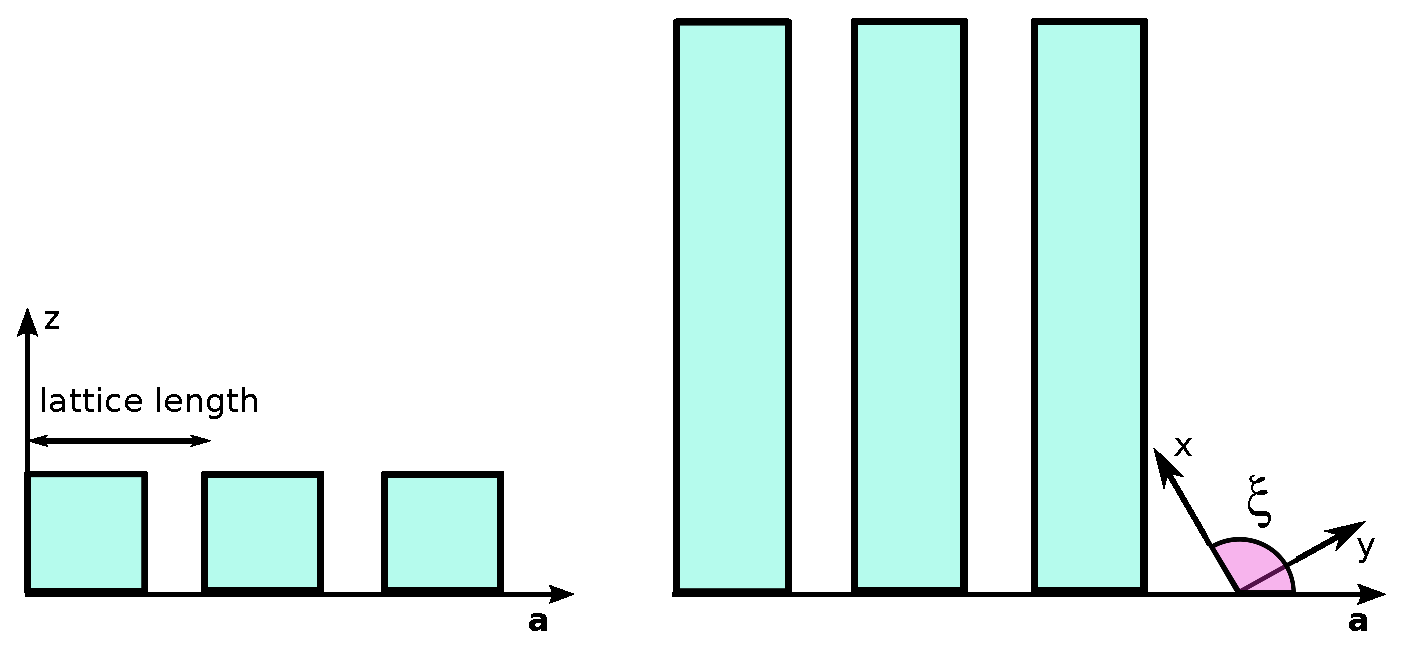
\includegraphics[width=0.75\textwidth]{Figures/drawing/1DGrating.eps}
\end{center}
\caption{Schematic representation of a 1D lattice (side and top views). Such a lattice is characterized by a lattice length and the angle $\xi$.}
\label{fig:1dgrating}
\end{figure}

\ImportantPoint{Remark:}{By default the long axis of the particles in this 1D lattice is along the beam axis. That is the reason why in the example below the particles are rotated by  $90^{\circ}$ in the $(x,y)$ plane: the main axis of the lattice is thefore parallel to the y-axis, perpendicular to the long axis of the particles.}

\vspace{12pt}
A probability distribution function \Code{pdf} has to be chosen from the list in section~\ref{baftd} in order to apply some modifications to the scattering peaks. This function is implemented using \Code{setProbabilityDistribution(pdf)}. 

\paragraph{Example:} Script~\ref{lst:1dlattinterf} details how to build in  \BornAgain\ a sample using\\ \Code{InterferenceFunction1DLattice} as the interference function. As mentioned previously, this interference function can only be used with infinitely wide or long particles.\\ Here the sample is made of infinitely long boxes deposited on a substrate (these particles are characterized by their widths and heights). They are also rotated by $90^{\circ}$  in the sample surface in order to have their long axis perpendicular to the input beam, which is along the $x$-axis.\\
 The lattice parameters (the lattice length and angle between the lattice main axis and the $x$-axis) are passed into the constructor of the interference function.

\newpage
\begin{lstlisting}[language=python, style=eclipseboxed,numbers=none,nolol,caption={\Code{Python} script to generate a sample made of infinitely long boxes deposited on a substrate layer with the 1DLatticeInterference function. The part specific to the interferences is marked in a red italic font.},label={lst:1dlattinterf}]
def get_sample():
    """
    Build and return the sample with 1DLatticeInterference function
    """
    # defining materials
    m_air = HomogeneousMaterial("Air", 0.0, 0.0)
    m_substrate = HomogeneousMaterial("Substrate", 6e-6, 2e-8)
    m_particle = HomogeneousMaterial("Particle", 6e-4, 2e-8)

    # collection of particles
    ff = FormFactorInfLongBox(10.*nanometer, 15.0*nanometer)
    box = Particle(m_particle, ff)
    particle_layout = ParticleLayout()
    transform = Transform3D.createRotateZ(90.0*degree)
    particle_layout.addParticle(box, transform)

    # interference function
    |interference = InterferenceFunction1DLattice(30.0*nanometer, 0.0*degree)|
    |pdf = FTDistribution1DCauchy(200./2./M_PI*nanometer)|
    |interference.setProbabilityDistribution(pdf)|
    |particle_layout.addInterferenceFunction(interference)|

    # air layer with particles and substrate form multi layer
    air_layer = Layer(m_air)
    air_layer.addLayout(particle_layout)
    substrate_layer = Layer(m_substrate, 0)

    multi_layer = MultiLayer()
    multi_layer.addLayer(air_layer)
    multi_layer.addLayer(substrate_layer)
    return multi_layer
\end{lstlisting} 

\newpage
\subsubsection{\ding{253} \Code{InterferenceFunctionRadialParaCrystal(peak\_distance, damping\_length)}}  
\begin{itemize}
\item[where] \Code{peak\_distance} is the average distance to the first neighbor peak, 
\item[]\Code{width} is the width parameter of the probability distribution,
\item[] \Code{damping\_length} is used to introduce finite size effects by applying a multiplicative coefficient equal to  $\exp$(-\Code{peak\_distance/damping\_length}) to the Fourier transform of the probability densities. \Code{damping\_length} is equal to 0 by default and, in this case, no correction is applied.
\end{itemize}

A probability distribution function \Code{pdf} has to be chosen from the list in section~\ref{baftd} in order to apply some modifications to the scattering peaks. This function is implemented using \Code{setProbabilityDistribution(pdf)}. 


\MakeRemark{Remark}{
This interference function is not one-dimensional.  It takes into account the radial componant of the scattering vector.
}

\paragraph{Example}
To illustrate the radial paracrystal interference function, we use the same sample as in the case without interference: half-spheres deposited on a substrate.

\begin{lstlisting}[language=python, style=eclipseboxed,numbers=none,nolol,caption={\Code{Python} script to define the radial paracrystal interference function between half-spheres, where \Code{trsphere} is of type \Code{Particle}.},label={lst:1dpara}]
    particle_layout = ParticleLayout()
    particle_layout.addParticle(trsphere, 0.0, 1.0)
    interference = InterferenceFunctionRadialParaCrystal(25.0*nanometer, 1e3*nanometer)
    pdf = FTDistribution1DGauss(7 * nanometer)
    interference.setProbabilityDistribution(pdf)
    particle_layout.addInterferenceFunction(interference)
\end{lstlisting}



\begin{figure}[ht]
\begin{center}
\includegraphics[angle=-90,width=0.5\textwidth]{Figures/gisasmap/HSphere_1DDL.pdf}
\end{center}
\caption{Output intensity scattered from a sample made of half-spheres with the radial paracrystal interference between them. This figure has been generated using Script~\ref{lst:1dpara} for the interference function.}
\label{fig:1ddl}
\end{figure}

\FloatBarrier

\newpage
\subsubsection{\ding{253}  \Code{InterferenceFunction2DLattice(L\_1, L\_2, alpha, xi)}} 
where ($L_1$, $L_2$, $\alpha$, $\xi$) are shown in figure~\ref{fig:2dlattice} with 
\begin{itemize}
\item[]$L_1$, $L_2$ the lengths of the lattice cell, 
\item[]$\alpha$ the angle between the lattice basis vectors $\mathbf{a}, \mathbf{b}$ in direct space,
\item[] $\xi$ is the angle defining the lattice orientation (set to $0$ by default); it is taken as the angle between the $\mathbf{a}$ vector of the lattice basis and the $\mathbf{x}$ axis of the reference cartesian frame (as shown in figure~\ref{fig:multil3d}).
\end{itemize}

\begin{figure}[ht]
\begin{center}
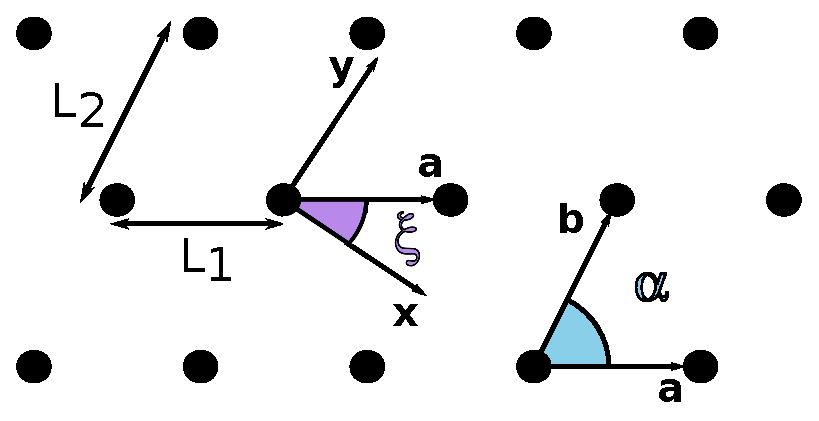
\includegraphics[width=0.5\textwidth]{Figures/drawing/2Dlattice.eps}
\end{center}
\caption{Schematic representation of a 2D lattice (top view). Such a lattice is characterized by lattice lengths $L_1$, $L_2$ and angles $\alpha$ and $\xi$.}
\label{fig:2dlattice}
\end{figure}

Like for the one-dimensional case, a probability distribution function \Code{pdf} has to be defined. One can choose between those listed in Section~\ref{baftd} and implements it using \Code{setProbabilityDistribution(pdf)}.

\paragraph{Example} The sample used to run the simulation is made of half-spheres deposited on a substrate. The interference function is "2Dlattice" and the particles are located at the nodes of a square lattice with $L_1=L_2=20$~nm, $\mathbf{a}\equiv \mathbf{b}$ and the probability distribution function is Gaussian. We also use the Decoupling Approximation. 

\begin{lstlisting}[language=python, style=eclipseboxed,numbers=none,nolol,caption={\Code{Python} script to define a 2DLattice interference function between hemi-spherical particles as well as the Decoupling Approximation in \Code{getSimulation()}.  The part specific to the interferences is marked in a red italic font.},label={lst:2dlatticeinterf}]
    #collection of particles
    sphere_ff = FormFactorTruncatedSphere(5*nanometer, 5*nanometer)
    sphere = Particle(m_particle, sphere_ff)
    |interference = InterferenceFunction2DLattice(20.0*nanometer, 20.0*nanometer, 90.0*degree, 0.0*degree)|
    |pdf = FTDistribution2DGauss(200.0*nanometer/2.0/M_PI, 75.0*nanometer/2.0/M_PI)|
    |interference.setProbabilityDistribution(pdf)|
    particle_layout = ParticleLayout()
    particle_layout.addParticle(sphere, 0.0, 1.0)
    |particle_layout.addInterferenceFunction(interference)|

    # interference approx chosen between: DA (default) and SSCA
    |particle_layout.setApproximation(ILayout.DA)|
\end{lstlisting}
 
%\begin{lstlisting}[language=python, style=eclipseboxed,numbers=none,nolol]
%def get_simulation():
%    """
%    Create and return GISAXS simulation with beam and detector
%    """
%    simulation = Simulation()
%    simulation.setDetectorParameters(100, 0.0*degree, 2.0*degree, 100, 0.0*degree, 2.0*degree, True)
%    simulation.setBeamParameters(1.0*angstrom, 0.2*degree, 0.0*degree)
%    return simulation
%\end{lstlisting}


\begin{figure}[ht]
\begin{center}
\includegraphics[angle=-90,width=0.5\textwidth]{Figures/gisasmap/HSphere_2Dlattice.pdf}
\end{center}
\caption{Output intensity scattered from a sample made of half-spheres with 2DLattice interference function in the Decoupling Approximation.}
\label{fig:2dlatticeintensity}
\end{figure}

\FloatBarrier

\newpage%{\cleardoublepage}
%%%%%%%%%%%%%%%%%%%%%%%%%%%%%%%%%%%%%%%
\subsubsection{\ding{253} \Code{InterferenceFunction2DParaCrystal(L\_1, L\_2, lattice\_angle, $\xi$, damping\_length)}} 
\begin{itemize}
\item[where] $L_1$, $L_2$ are the lengths of the lattice cell,
\item[] lattice\_angle the angle between the lattice basis vectors $\mathbf{a}, \mathbf{b}$ in direct space,
\item[] $\xi$ is the angle defining the lattice orientation (set to $0$ by default).
\item[] \Code{damping\_length} is used to introduce finite size effects by applying a multiplicative coefficient equal to  $\exp$(-\Code{peak\_distance/damping\_length}) to the Fourier transform of the probability densities. \Code{damping\_length} is equal to 0 by default and, in this case, no correction is applied.
\end{itemize}
Two predefined interference functions can also be used:
\begin{itemize}
\item  \Code{createSquare(peak\_distance, damping\_length, domain\_size\_1, domain\_size\_2)}\\
where the angle between the base vectors of the lattice is set to $\pi/2$,
it creates a squared lattice,
\item \Code{createHexagonal(peak\_distance, damping\_length, domain\_size\_1, domain\_size\_2)}\\
where the angle between the base vectors of the lattice is set to $2\pi/3$ ,
\end{itemize}
where
\Code{domain\_size1, 2} are the dimensions of coherent domains of the paracrystal along the main axes,\\ \Code{peak\_distance} is the same in both directions and $\mathbf{a}\equiv \mathbf{x}$.\\

Probability distribution functions have to be defined. As the two-dimensional paracrystal is defined from two independent one-dimensional paracrystals, we need two of these functions, using\\ \Code{setProbabilityDistributions(pdf\_1, pdf\_2)}, with \Code{pdf\_{1,2}} related to each main axis of the paracrystal (see figure~\ref{fig:2dparaschematic}).


\begin{figure}[ht]
\begin{center}
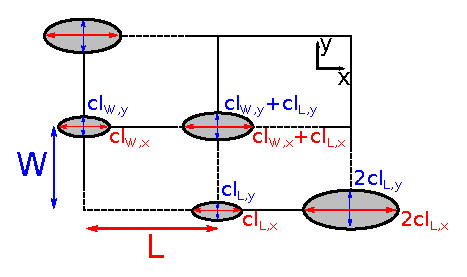
\includegraphics[width=0.75\textwidth]{Figures/drawing/drawing2Dparacrystal.eps}
\end{center}
\caption{Shematics of the ideal 2D paracrystal. The grey-shaded areas mark the regions where the probability to find a node is larger that the width at half-maximum of the distribution. $L$ and  $W$ are the mean inter-node distances along the two crystallographic axes. cl$_{(L,W),(x,y)}$ are the widths of the distribution of distance. The disorder is propagated as we add more nodes. Such a structure would be generated using \Code{InterferenceFunction2DParacrystal(L,W,90.*degrees,0,damp\_length)}, with \Code{pdf$_1$ = FTDistribution2DGauss(cl$_{L,x}$,cl$_{L,y}$)} and  \Code{pdf$_2$ = FTDistribution2DGauss(cl$_{W,x}$,cl$_{W,y}$)}.}
\label{fig:2dparaschematic}
\end{figure}


\paragraph{Example} The particles deposited on a substrate are half-spheres. The scattered beams interference via the 2DParacrystal distribution function. The paracrystal is based on a 2D hexagonal lattice with a Gaussian probability distribution function in reciprocal space.  Script~\ref{lst:2dparainterf} shows the implementation of the interference function and fig.~\ref{fig:2ddl} an example of output intensity using hemi-spherical particles.

\begin{lstlisting}[language=python, style=eclipseboxed,numbers=none,nolol,caption={\Code{Python} script to define a "2DParacrystal" interference function between particles forming an hexagonal monolayer. },label={lst:2dparainterf}]
    interference = InterferenceFunction2DParaCrystal.createHexagonal(30.0*nanometer,0.0, 40.0*micrometer, 40.0*micrometer)|
    pdf = FTDistribution2DCauchy(1.0*nanometer, 1.0*nanometer)
    interference.setProbabilityDistributions(pdf, pdf)
    particle_layout.addInterferenceFunction(interference)
\end{lstlisting}

\begin{figure}[ht]
\begin{center}
\includegraphics[angle=-90,width=0.5\textwidth]{Figures/gisasmap/HSphere_2DDL.pdf}
\end{center}
\caption{Output intensity scattered from a sample made of half-spheres with 2DParacrystal interference function.}
\label{fig:2ddl}
\end{figure}

\FloatBarrier

\subsection{Summary}
\begin{table}[h]
\begin{tabular}{lll}
\hline
Name & Characteristics &  Comments \\
\hline
DA & no correlations& implemented with \Code{setApproximation} \\
     & & default option \\
\hline
LMA & sample = groups of particles & automatic implementation if several \\ 
 & of identical sizes and shapes & \Code{ParticleLayout}s are defined \\
\hline
SSCA & distance between particles =  &  - implemented with \Code{setApproximation} \\
 &function of their sizes&  - dimensionless coupling coefficient $\kappa$ is \\
 & & required using \Code{setKappa}.\\
\hline
\hline
\end{tabular}
\caption{List of size-distribution models implemented in \BornAgain.}
\end{table}

\FloatBarrier

\begin{landscape}
\begin{table}
\begin{tabular}{lll}
\hline
Function  & Parameters & Comments\\
\hline
\Code{InterferenceFunctionNone}  & None & disordered distribution \\
\hline
\Code{InterferenceFunction1DLattice} & \Code{lattice\_length} & use only with infinitely long/wide particles \\
  & $\xi=\widehat{(\mathbf{x},\mathbf{a})}$ & pdf=(Cauchy, Gauss or Voigt)  to be defined\\
\hline
 \Code{InterferenceFunctionRadialParaCrystal}  & peak\_distance of pdf & pdf=(Cauchy, Gauss or Voigt) to be defined \\
& damping\_length (optional) & \\
\hline
 \Code{InterferenceFunction2DLattice}  & L\_1, L\_2: lattice lengths & pdf=(Cauchy, Gauss or Voigt) to be defined\\
                        & lattice\_angle=$\widehat{(\mathbf{a},\mathbf{b})}$ & \\
                                                            & $\xi =\widehat{(\mathbf{x},\mathbf{a})}$ & \\                                                  
\hline
\Code{InterferenceFunction2DParaCrystal}  & L\_1, L\_2: lattice lengths & 2D pdf=(Cauchy, Gauss or Voigt) to be defined \\
                          & lattice\_angle=$\widehat{(\mathbf{a},\mathbf{b})}$ & (1 pdf per axis) \\
& $\xi=\widehat{(\mathbf{x},\mathbf{a})}$ & \\
& damping\_length (optional)  &  same for both axes\\
\hline
\hline
\end{tabular}
\caption{List of interference functions implemented in \BornAgain. pdf : probability distribution function, $\mathbf{a}, \mathbf{b}$ are the lattice base vectors, and $\mathbf{x}$ is the axis vector perpendicular to the detector plane.}
\end{table}
\end{landscape}


%%%%%%%%%%%%%%%%%%%%%%%%%%%%%%%%%%%%%%%%%%%%%%%%%%%%%%%%%%%%%%%%%%%%%%%%%%%%%%%%
\section{Particles - Form factors} \SecLabel{sect:ff}
%%%%%%%%%%%%%%%%%%%%%%%%%%%%%%%%%%%%%%%%%%%%%%%%%%%%%%%%%%%%%%%%%%%%%%%%%%%%%%%%

\subsection{Born approximation}

In \BornAgain\ the form factor is defined using the Born approximation as
\begin{equation}
F(\mathbf{q})=\int_V \exp (i\mathbf{q}.\mathbf{r}) d^3 \mathbf{r},
\label{ffformulaBA}
\end{equation}
where $V$ is the volume of the particle,
$\mathbf{q}=\mathbf{k}_i - \mathbf{k}_f$ is the scattering vector with
$\mathbf{k}_f$ and $\mathbf{k}_i$ the scattered and incident wave
vector, respectively.\\

The particle's shape is parametrized in a cartesian frame, with its
$z$-axis pointing upwards and its origin at the center of the bottom
of the particle: $\mathbf{r}=(x,y,z)$. 

All form factors have been implemented with complex scattering vectors
in order to take any material absorption into account.

Table~\ref{tab:formfactors} lists the shapes whose form
factors have been implemented in \BornAgain\ and a detailed description is given in Appendix \ref{appendixff}.

\newpage

\begin{table}[H] 
\caption{Table of form factors implemented in \BornAgain.} \label{tab:formfactors}
  \begin{tabulary} {\textwidth}{Lc Lc L c L} 
\hline 
Box,\phantom{-} \SecRef{Box} & & Prism3,  \SecRef{Prism3} & & Tetrahedron, \SecRef{Tetrahedron} & & Prism6,  \SecRef{Prism6}\\
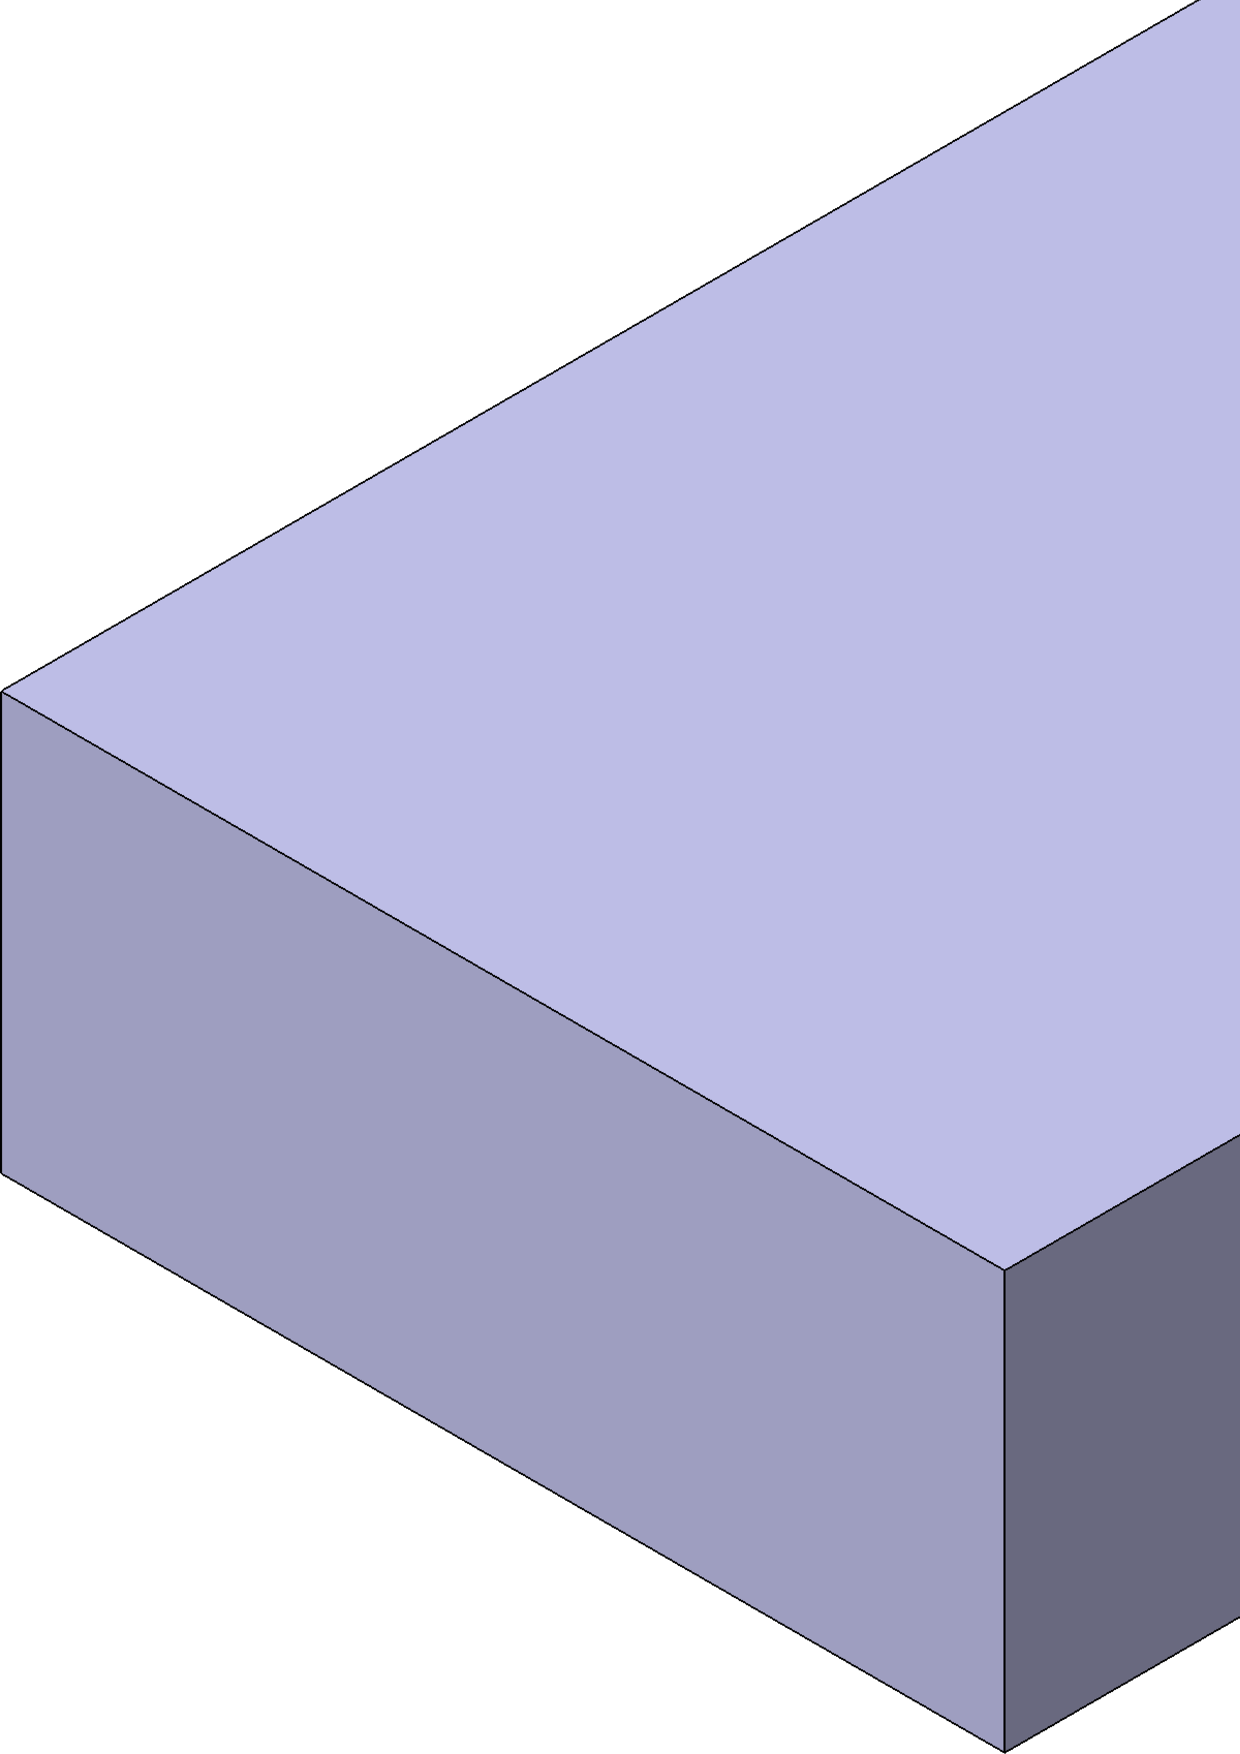
\includegraphics[width=1in]{Figures/blue/Box3d.png} & & 
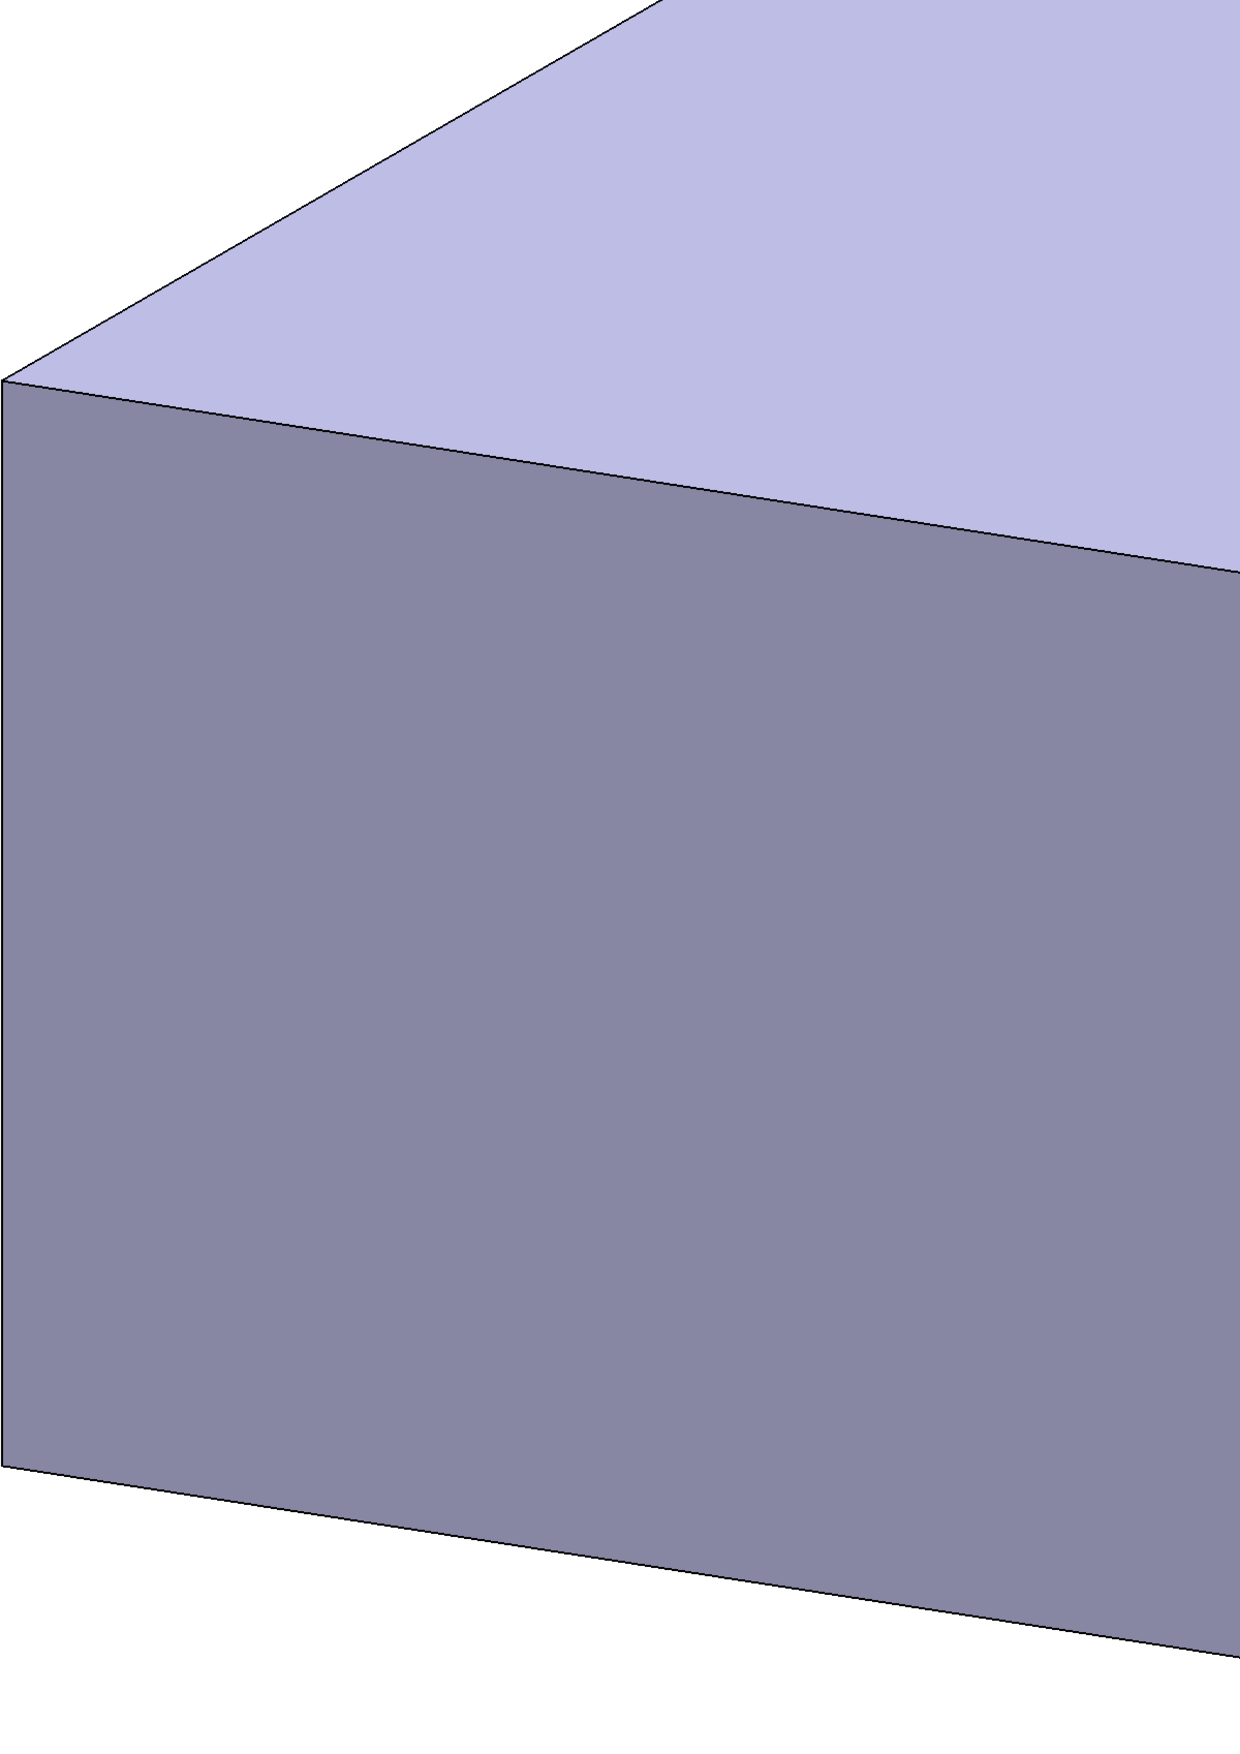
\includegraphics[width=1in]{Figures/blue/Prism33d.png} & & 
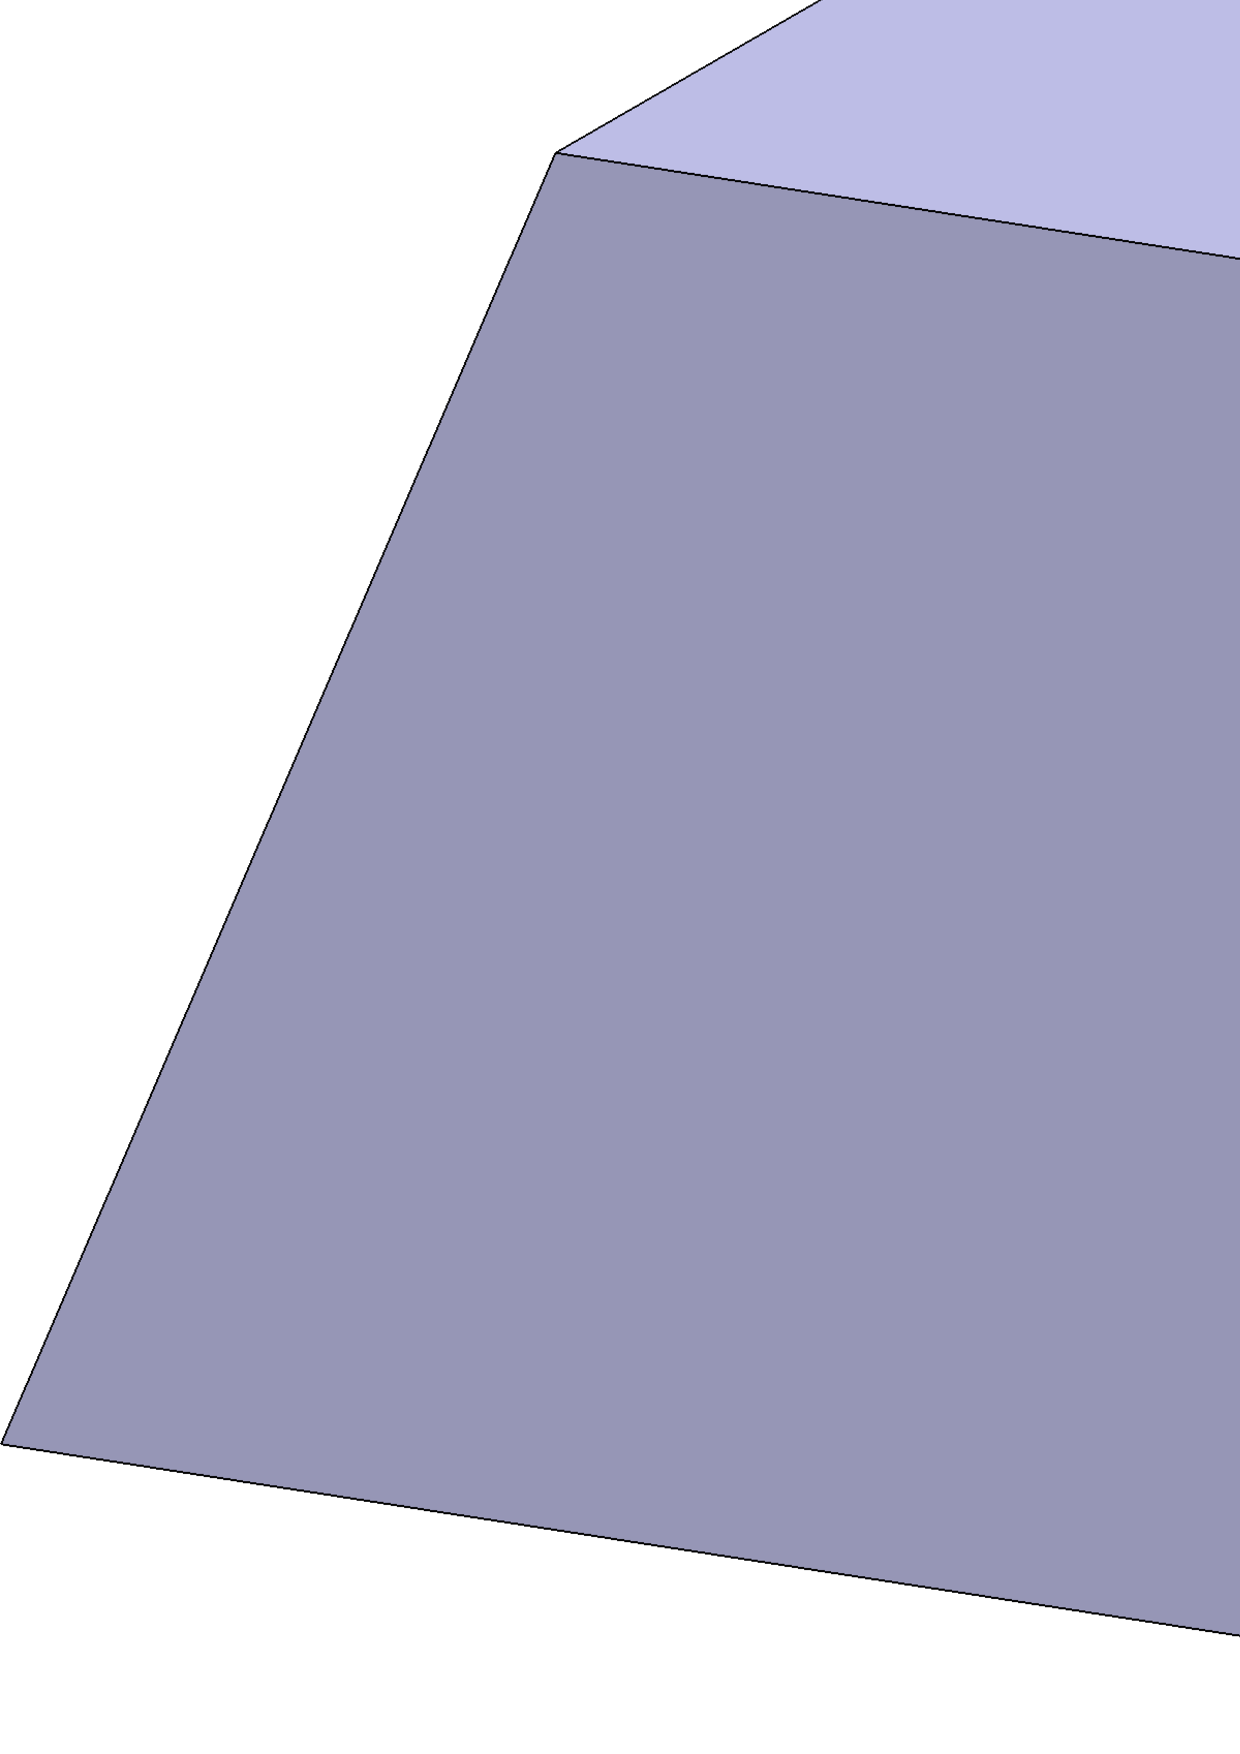
\includegraphics[width=1in]{Figures/blue/Tetrahedron3d.png} & & 
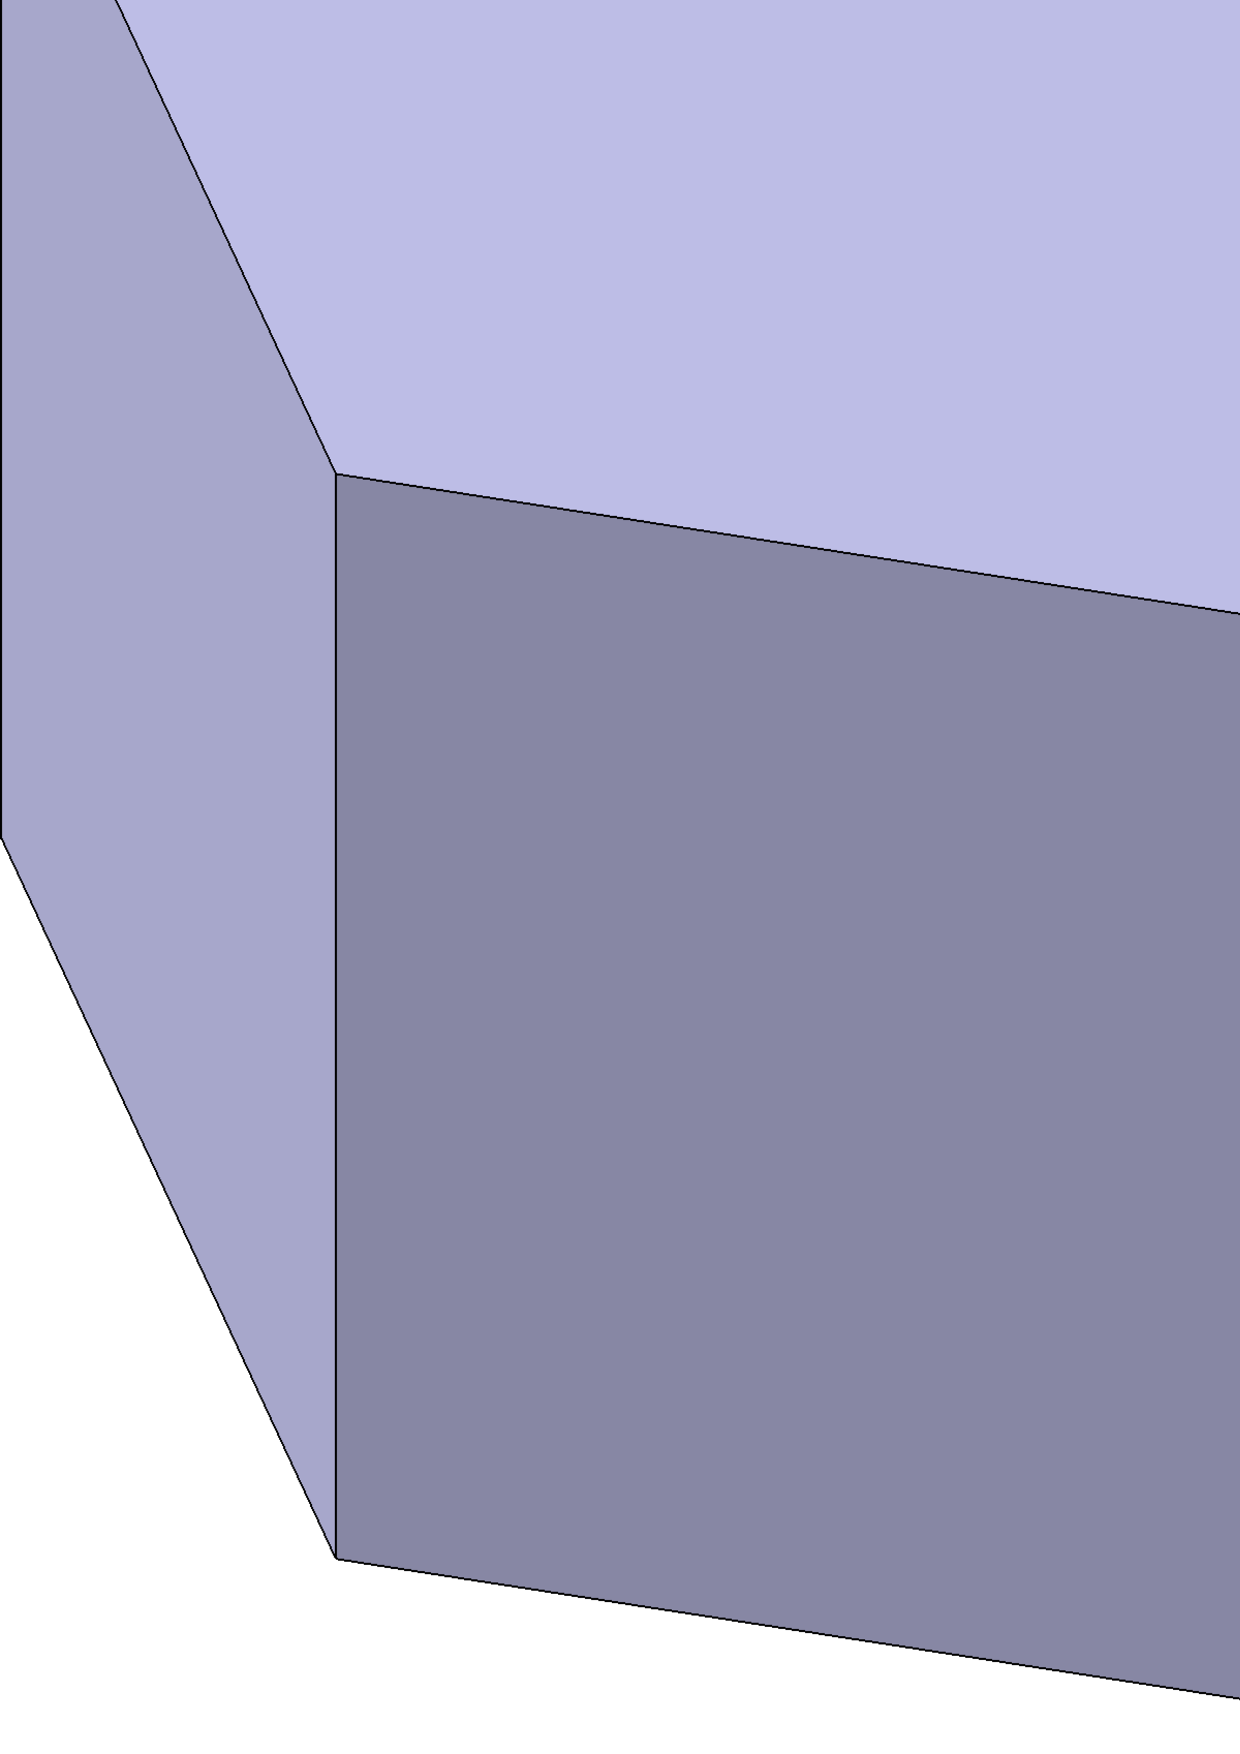
\includegraphics[width=1in]{Figures/blue/Prism63d.png} 
\\
\hline 
Cone6,  \SecRef{Cone6} & &  Pyramid, \SecRef{Pyramid} & & Anisotropic pyramid,  \SecRef{AnisoPyramid} & &  {Cuboctahedron}, \SecRef{Cuboctahedron}\\
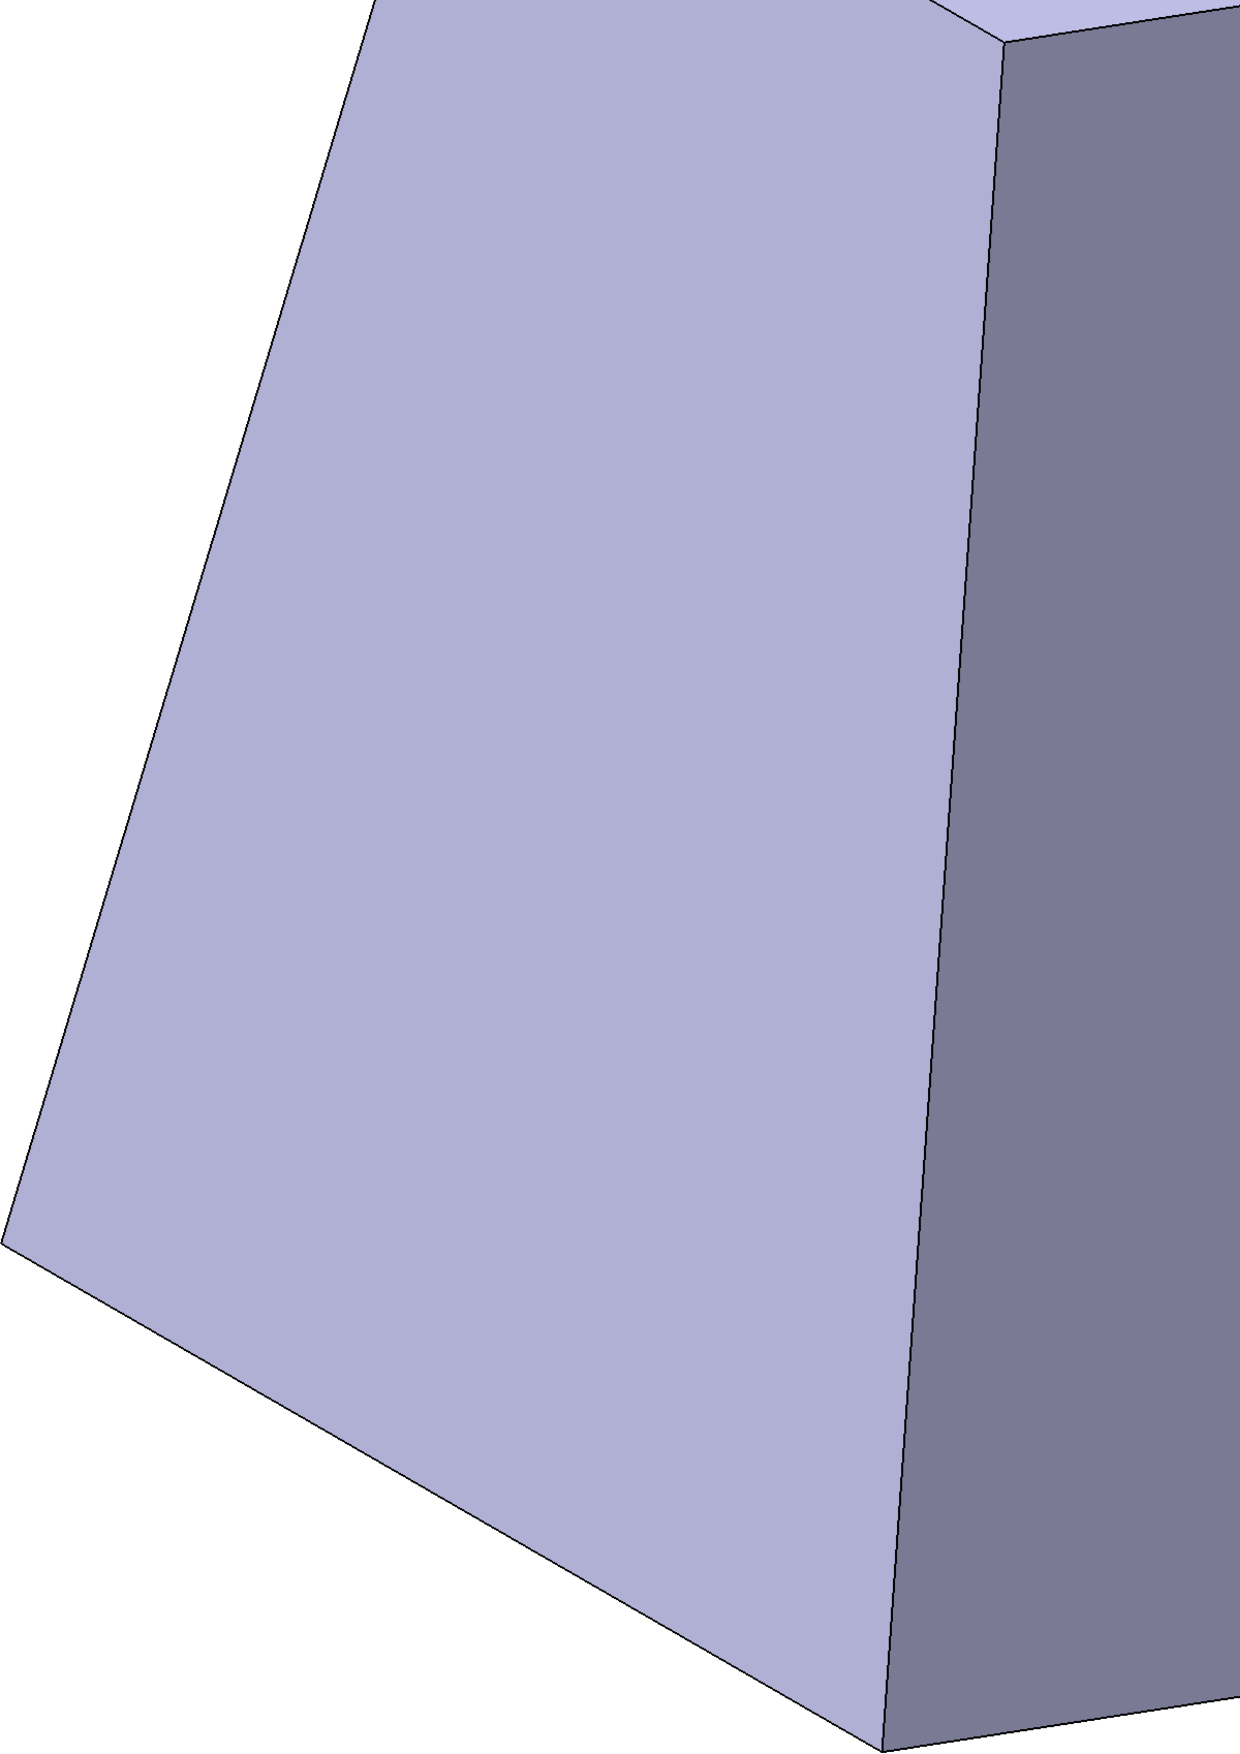
\includegraphics[width=1in]{Figures/blue/Cone63d.png}  & & 
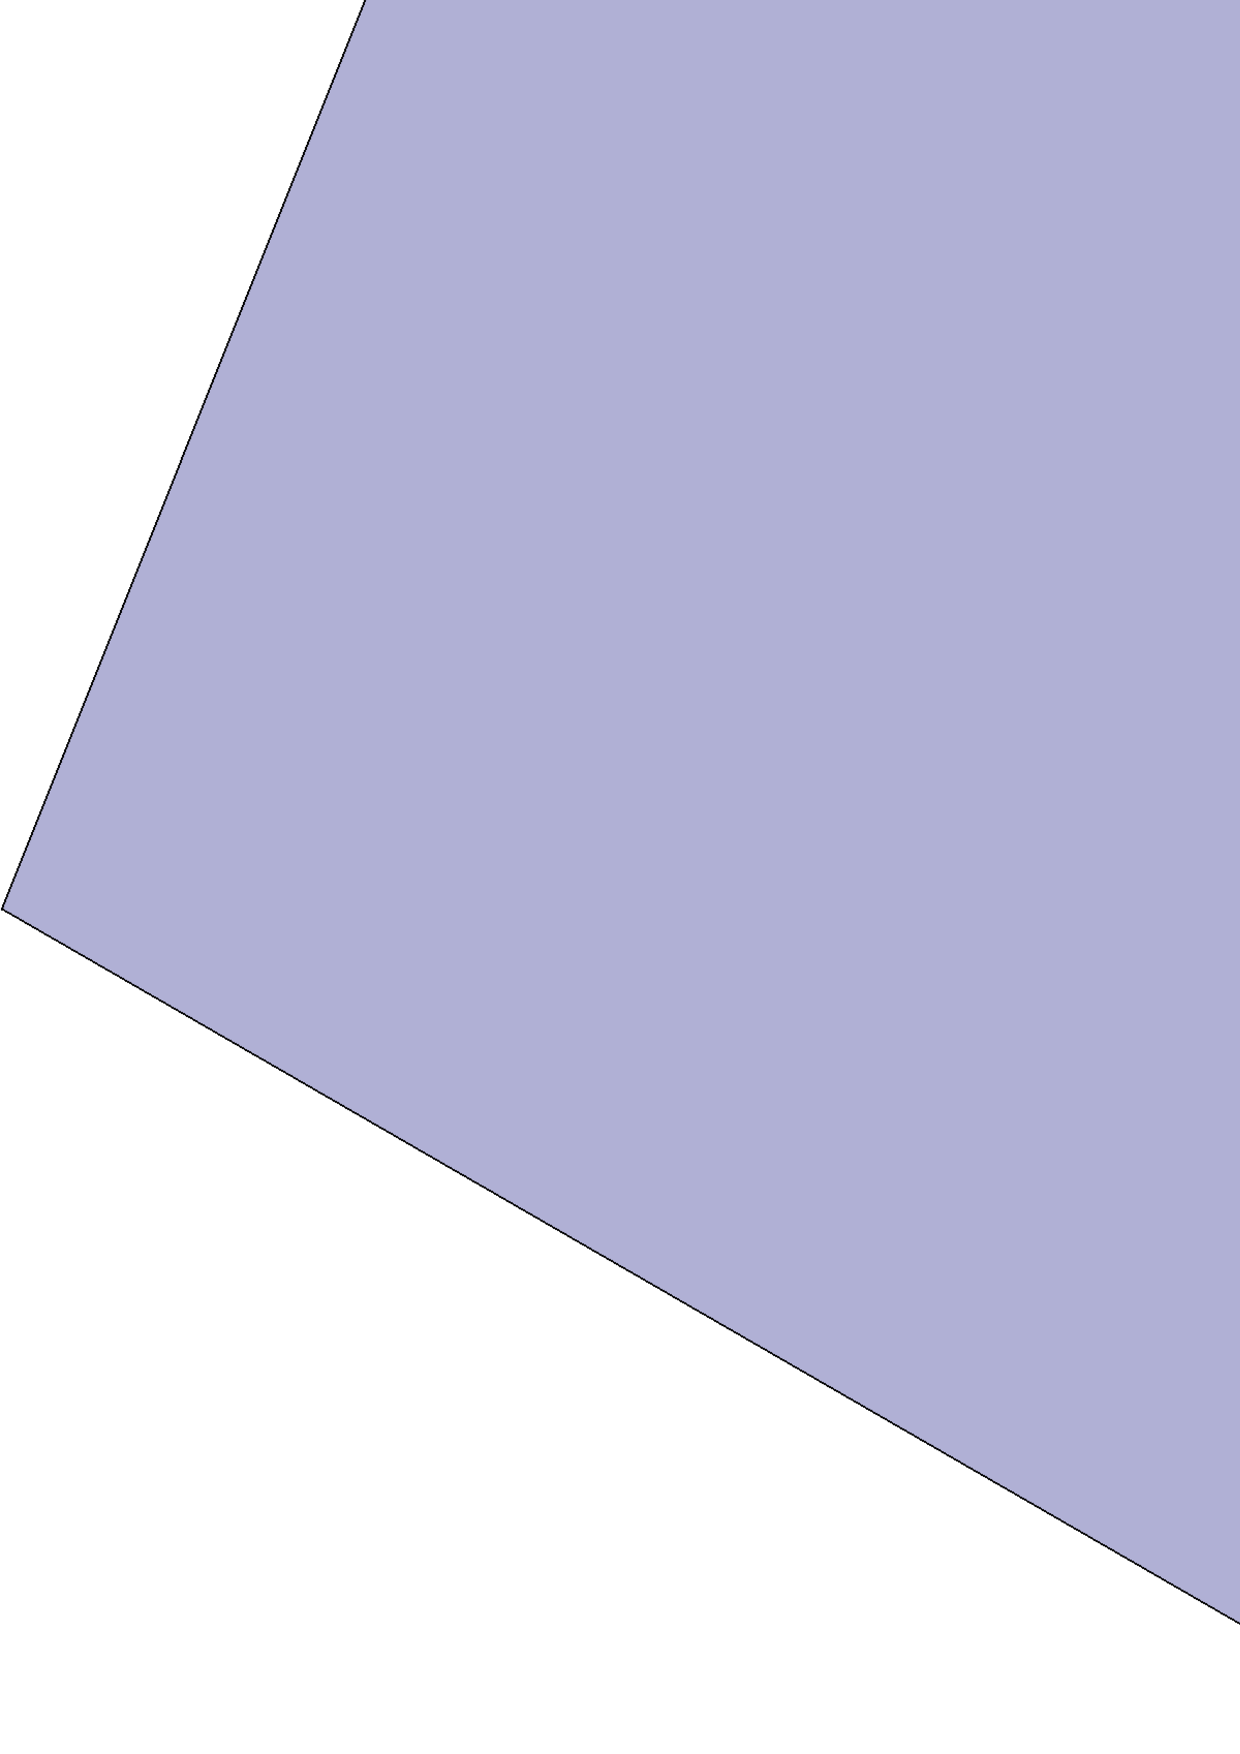
\includegraphics[width=1in]{Figures/blue/Pyramid3d.png} & &
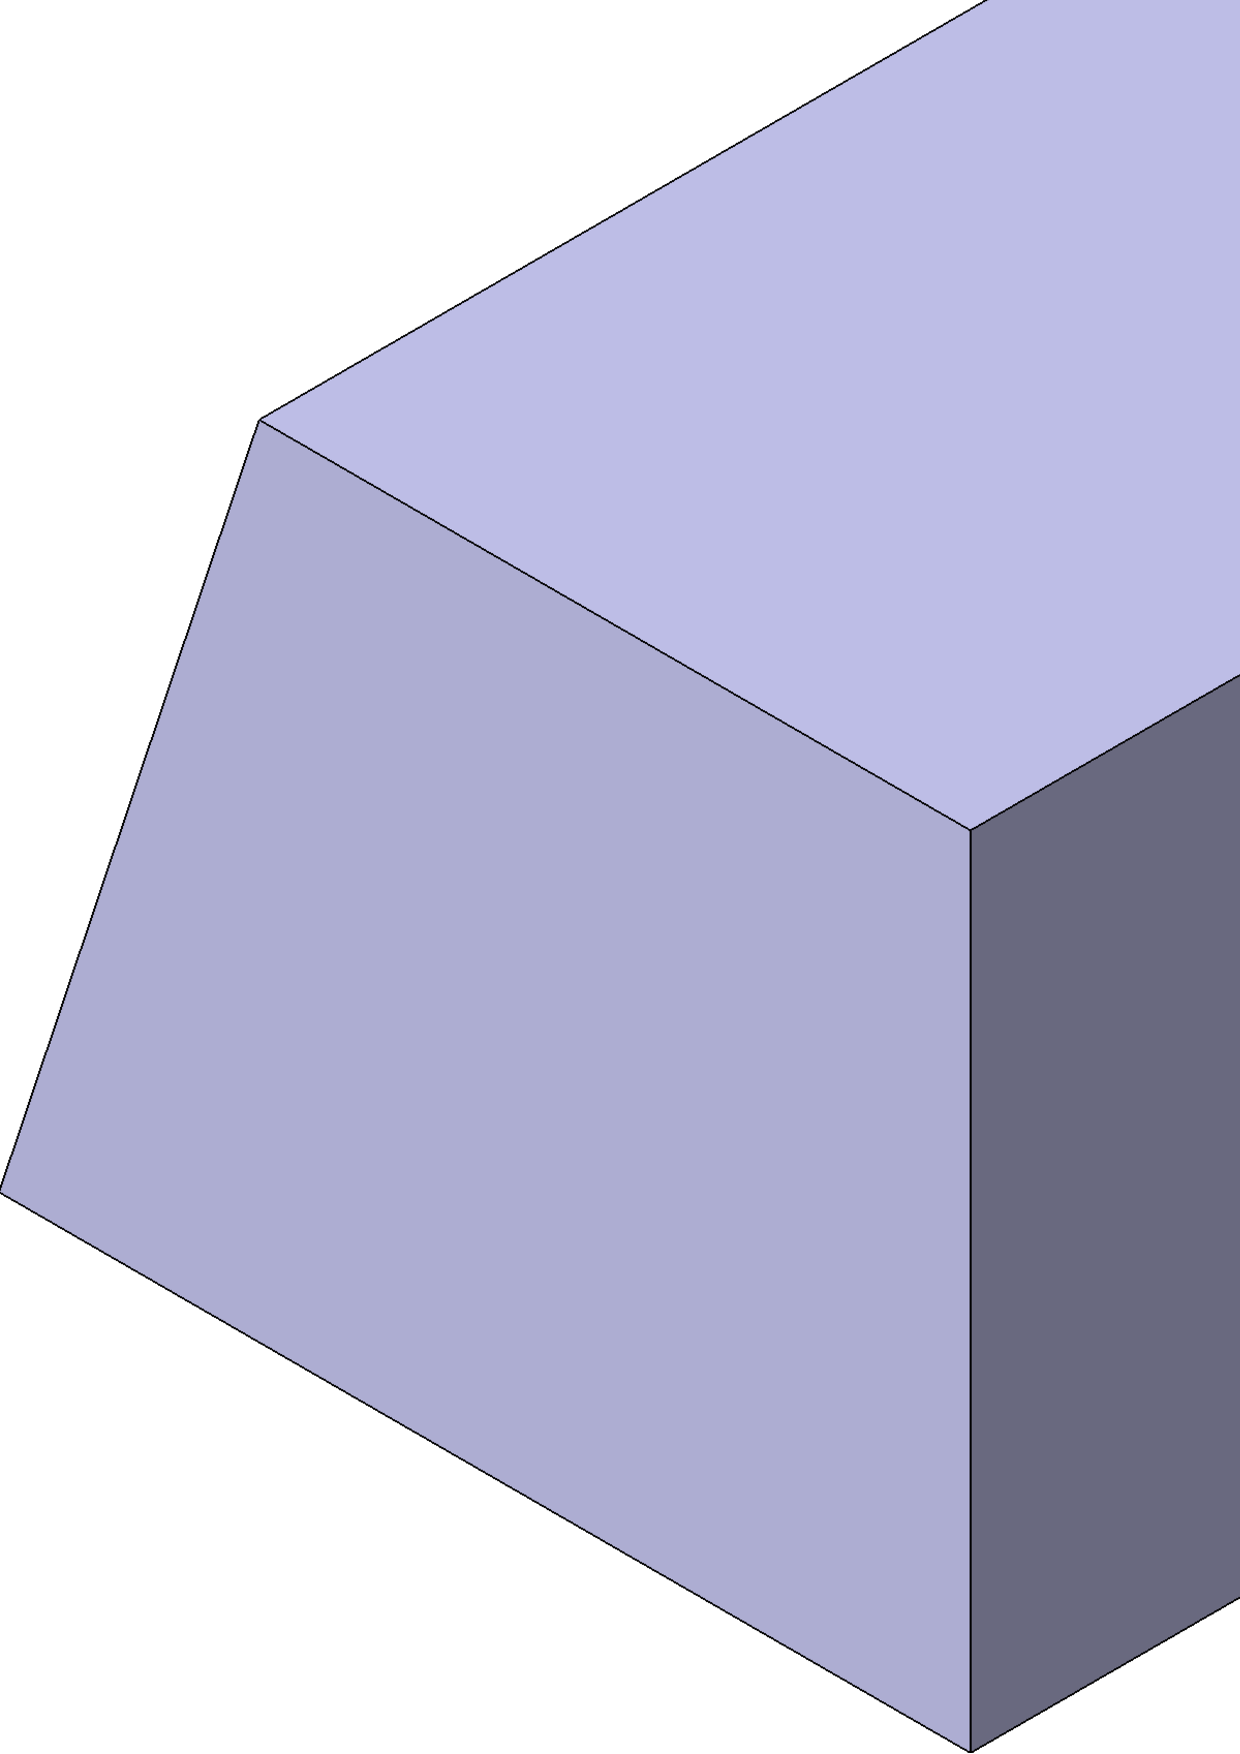
\includegraphics[width=1in]{Figures/blue/AnistropicPyramid3d.png} & & 
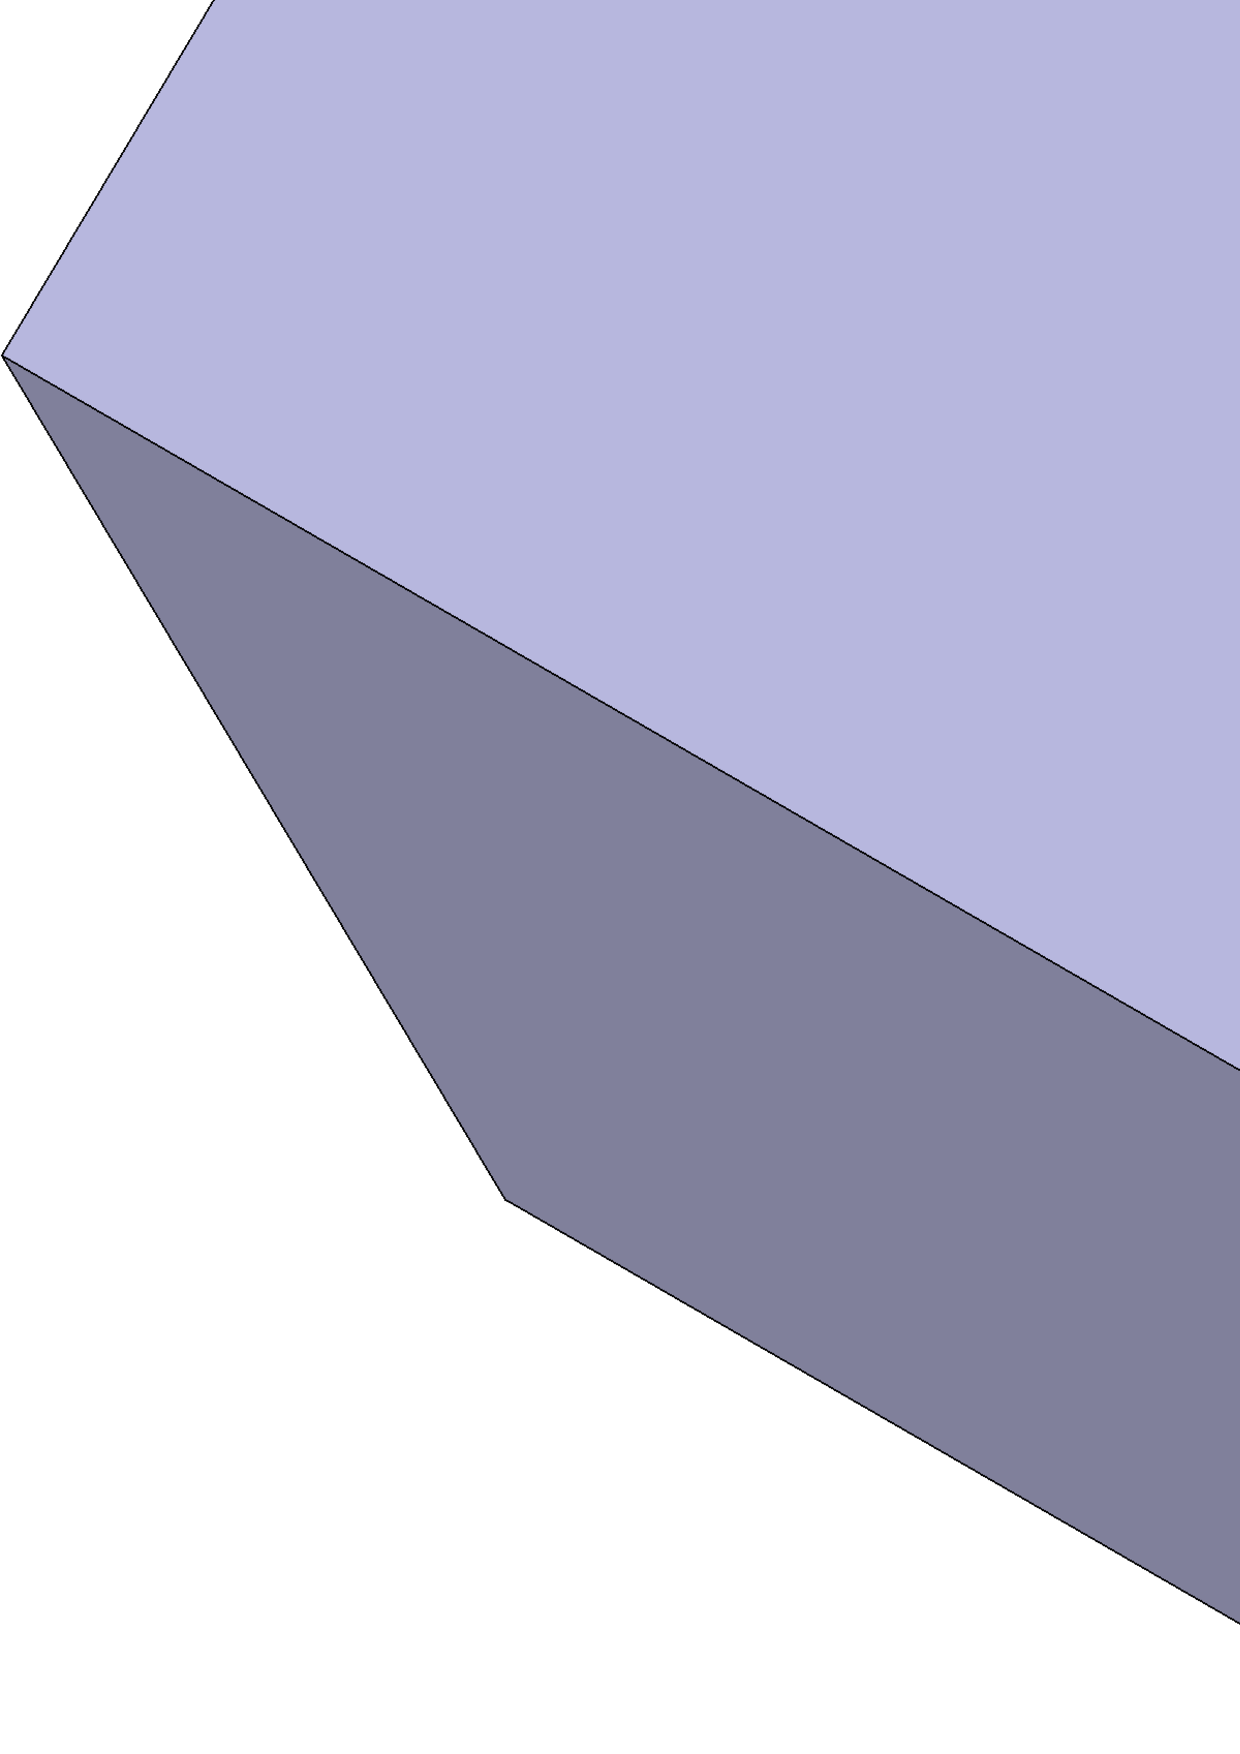
\includegraphics[width=1in]{Figures/blue/Cuboctahedron3d.png}
\\
\hline
Cylinder, \SecRef{Cylinder}  & & Ellipsoidal cylinder, \SecRef{EllipsoidalCylinder} & &  Cone,\phantom{--} \SecRef{Cone} & & Full Sphere, \SecRef{FullSphere} \\
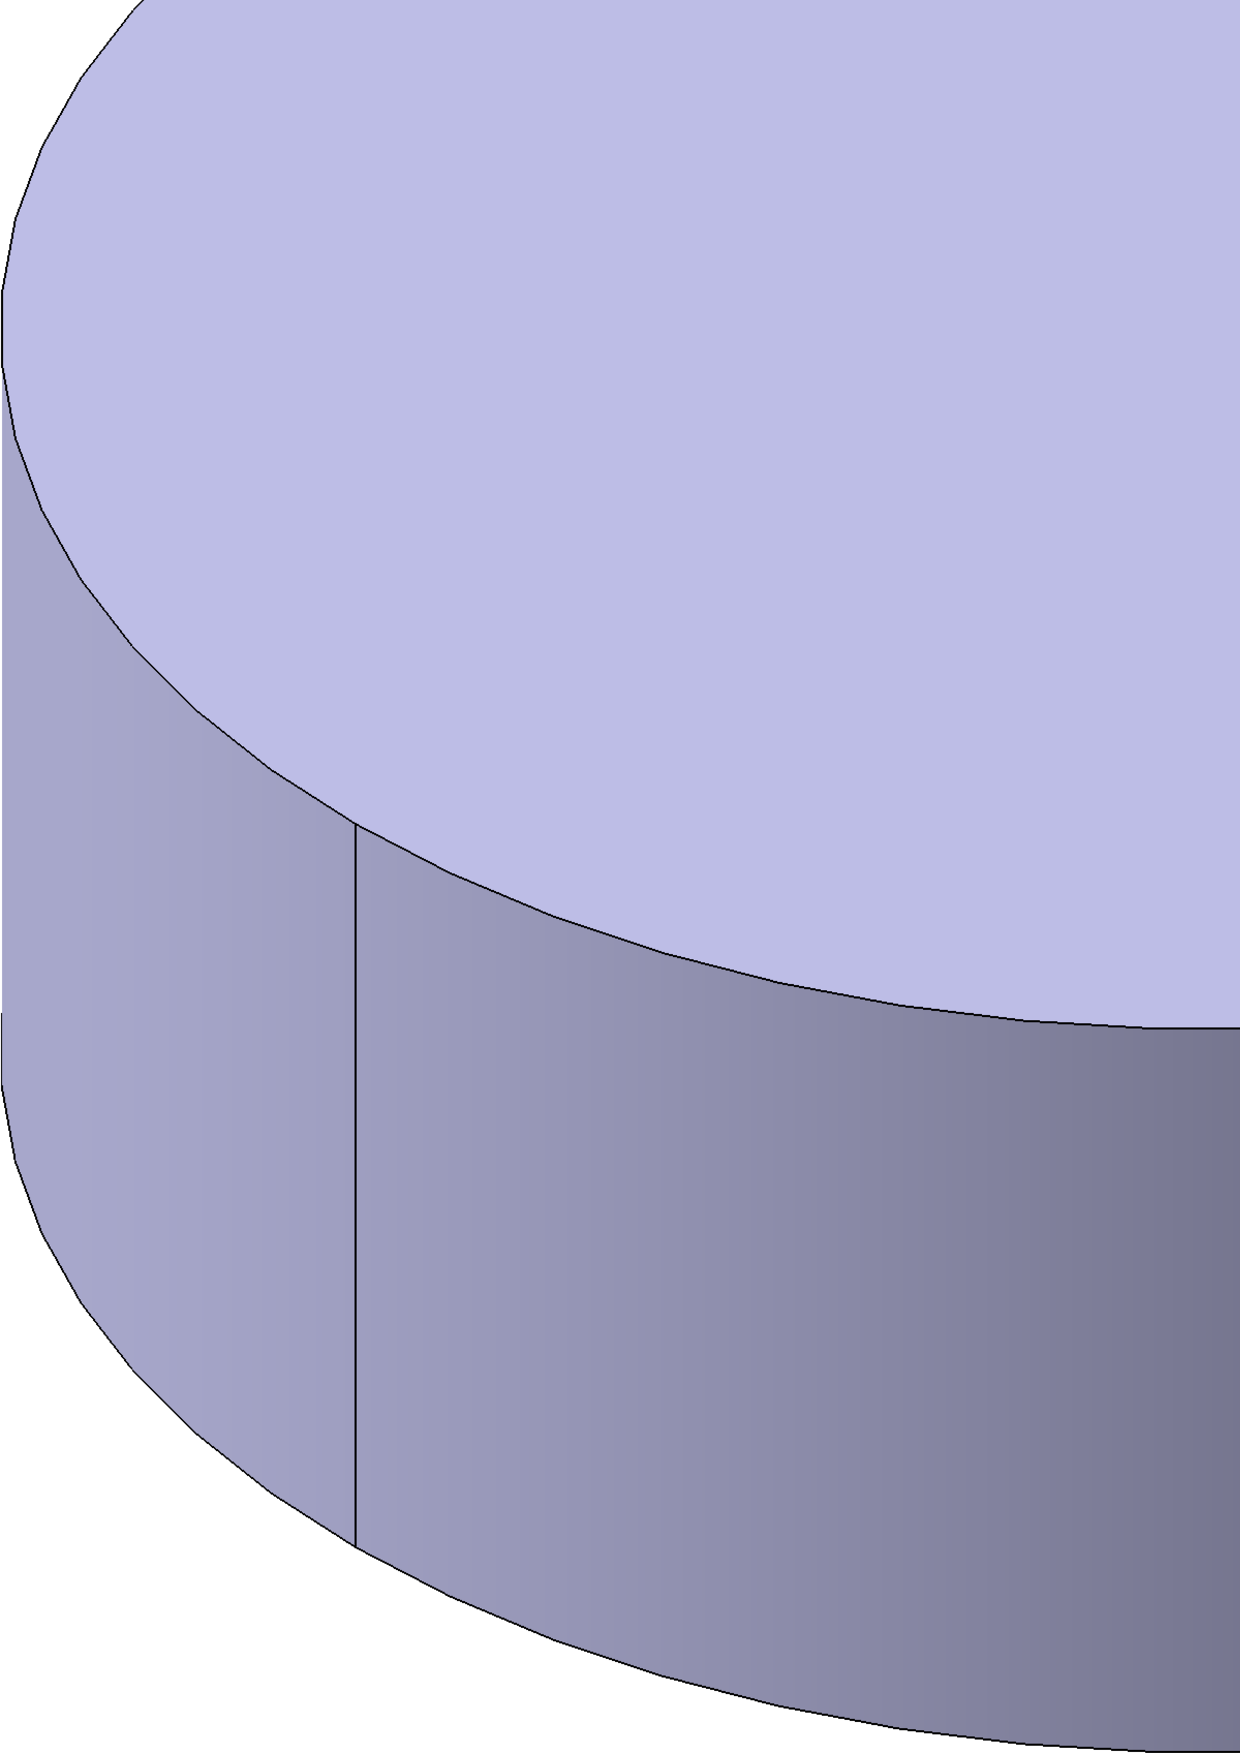
\includegraphics[width=1in]{Figures/blue/Cylinder3d.png} & & 
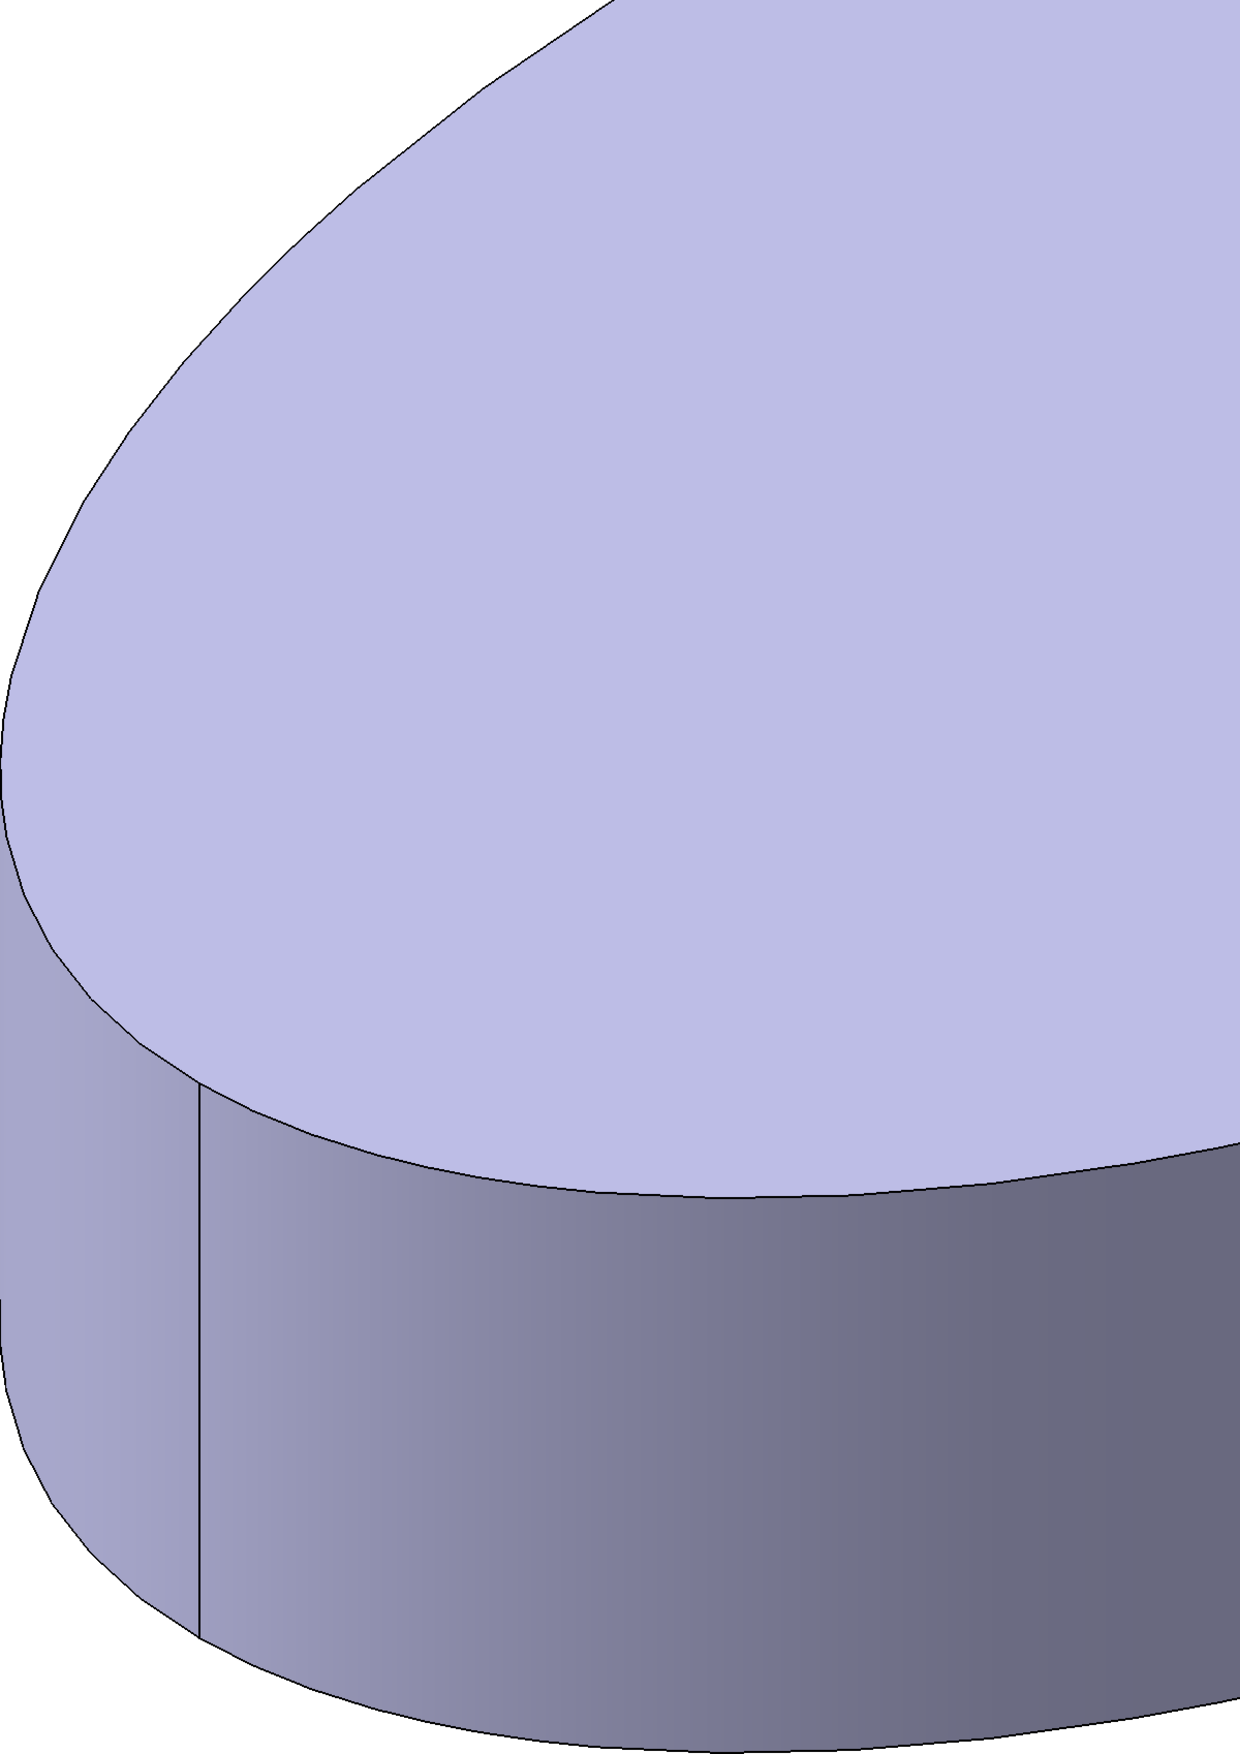
\includegraphics[width=1in]{Figures/blue/EllipsoidalCylinder3d.png} & & 
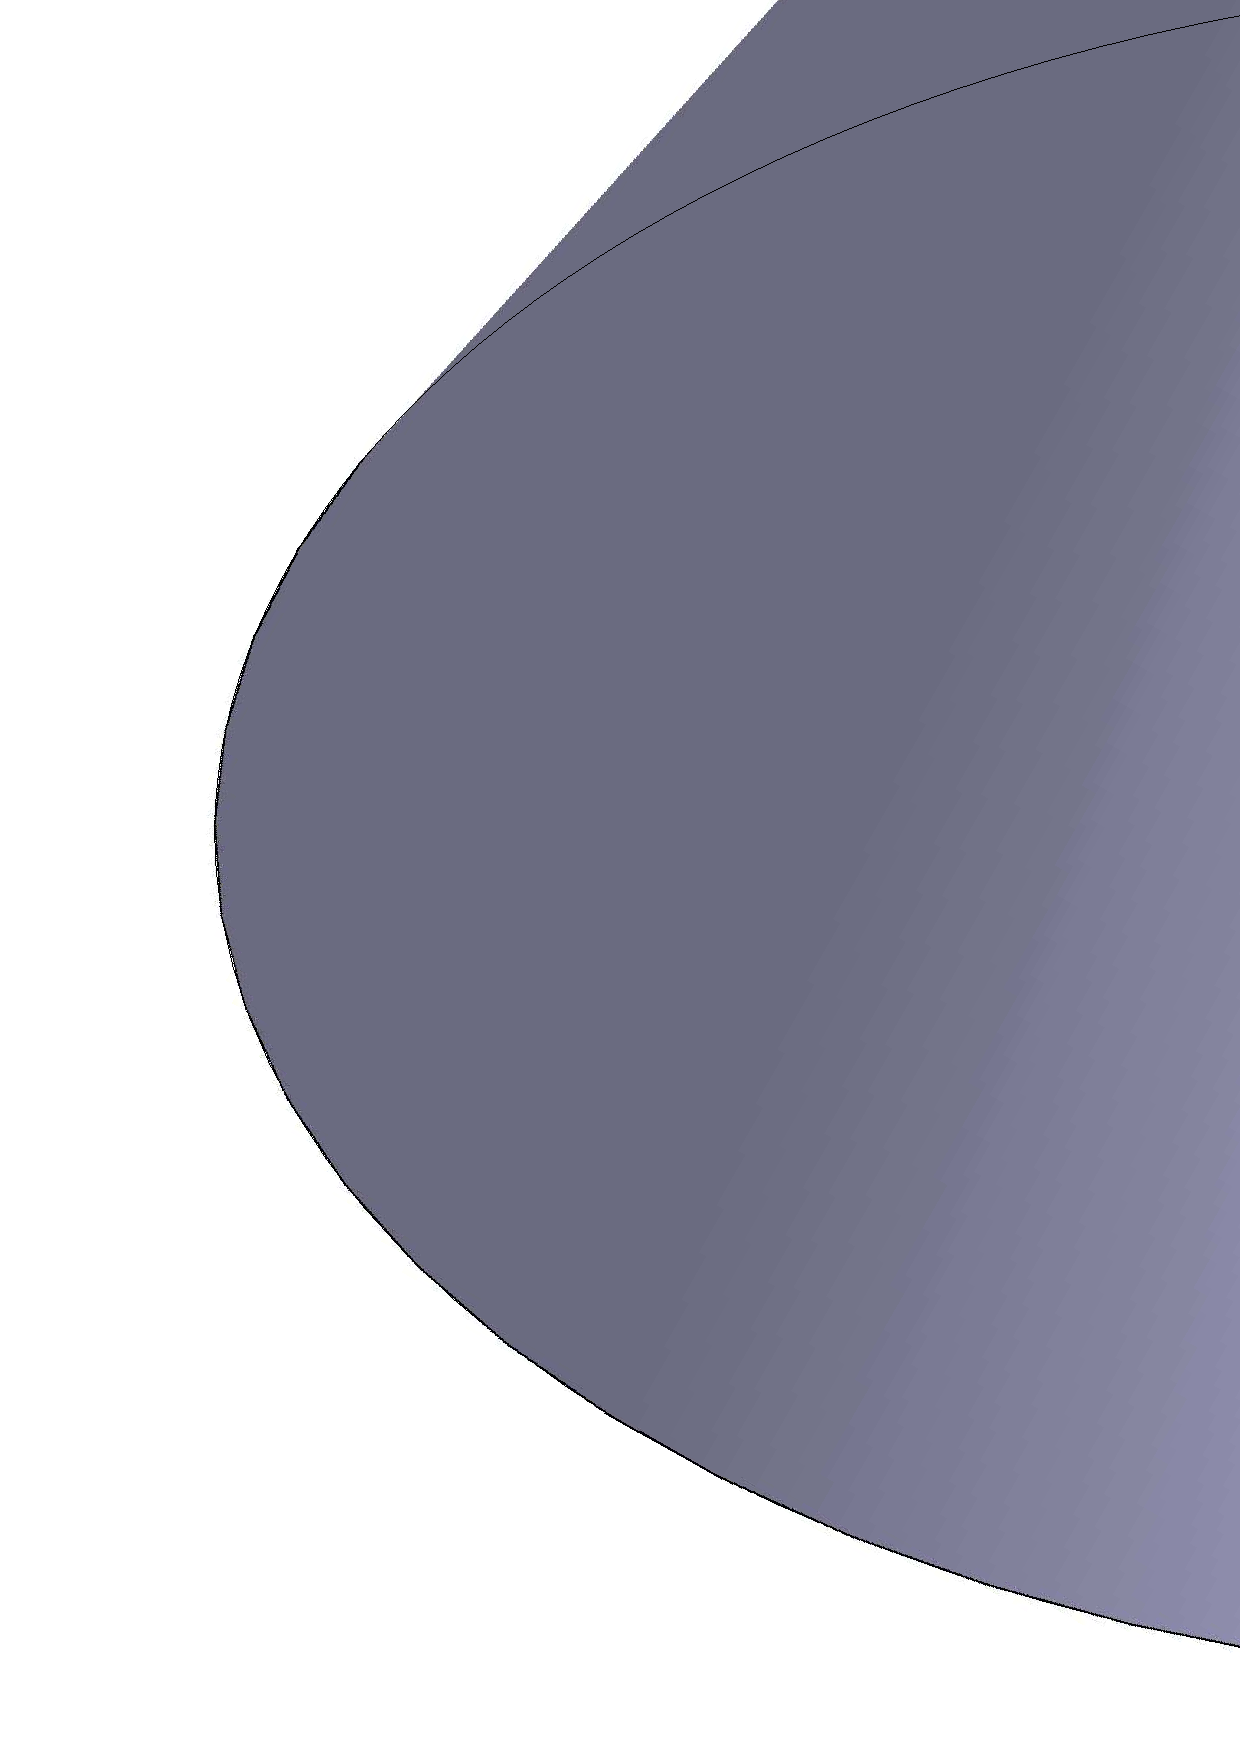
\includegraphics[width=1in]{Figures/blue/Cone3d.png} & & 
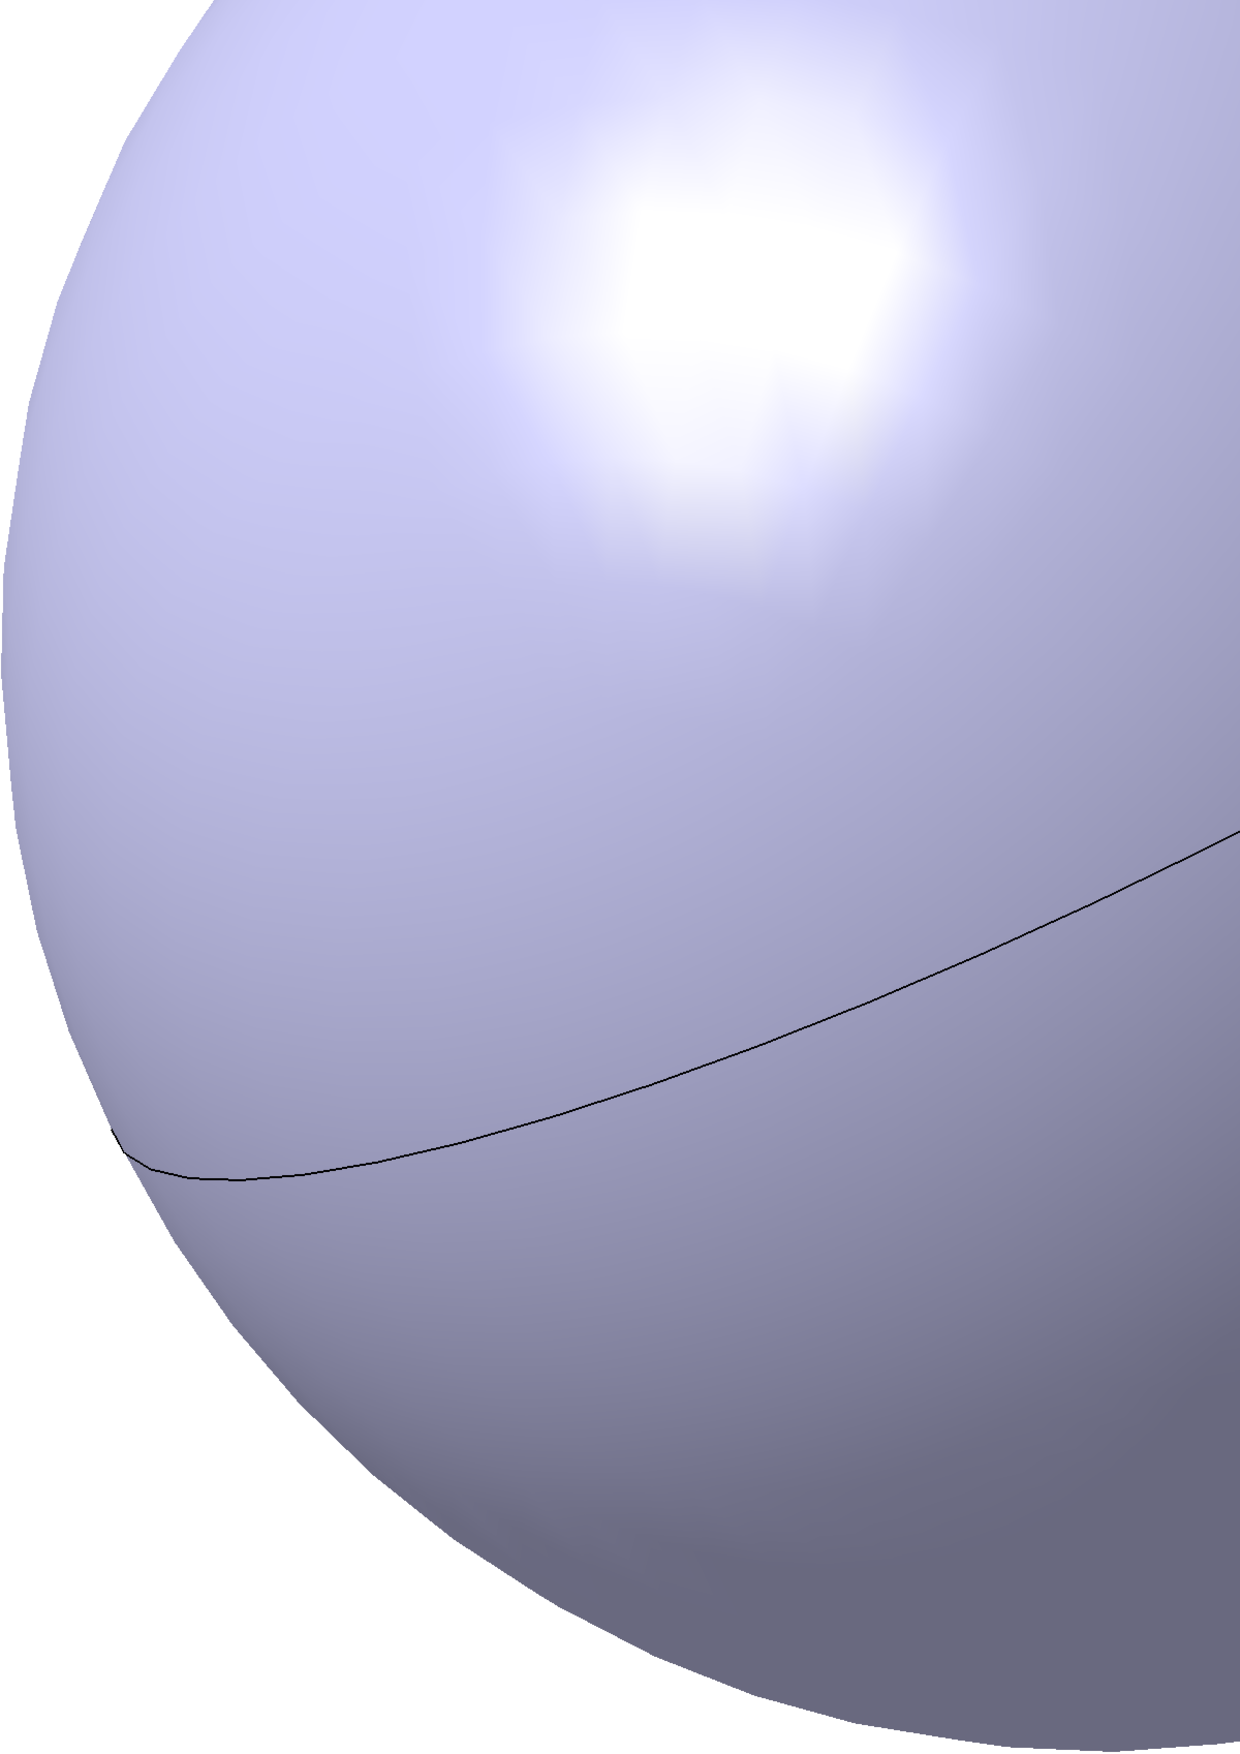
\includegraphics[width=1in]{Figures/blue/FullSphere3d.png} \\
\hline
Truncated Sphere, \SecRef{Sphere}  & & Full Spheroid, \SecRef{FullSpheroid} & & Truncated Spheroid,  \SecRef{Spheroid} & & Hemi Ellipsoid, \SecRef{HemiEllipsoid}\\
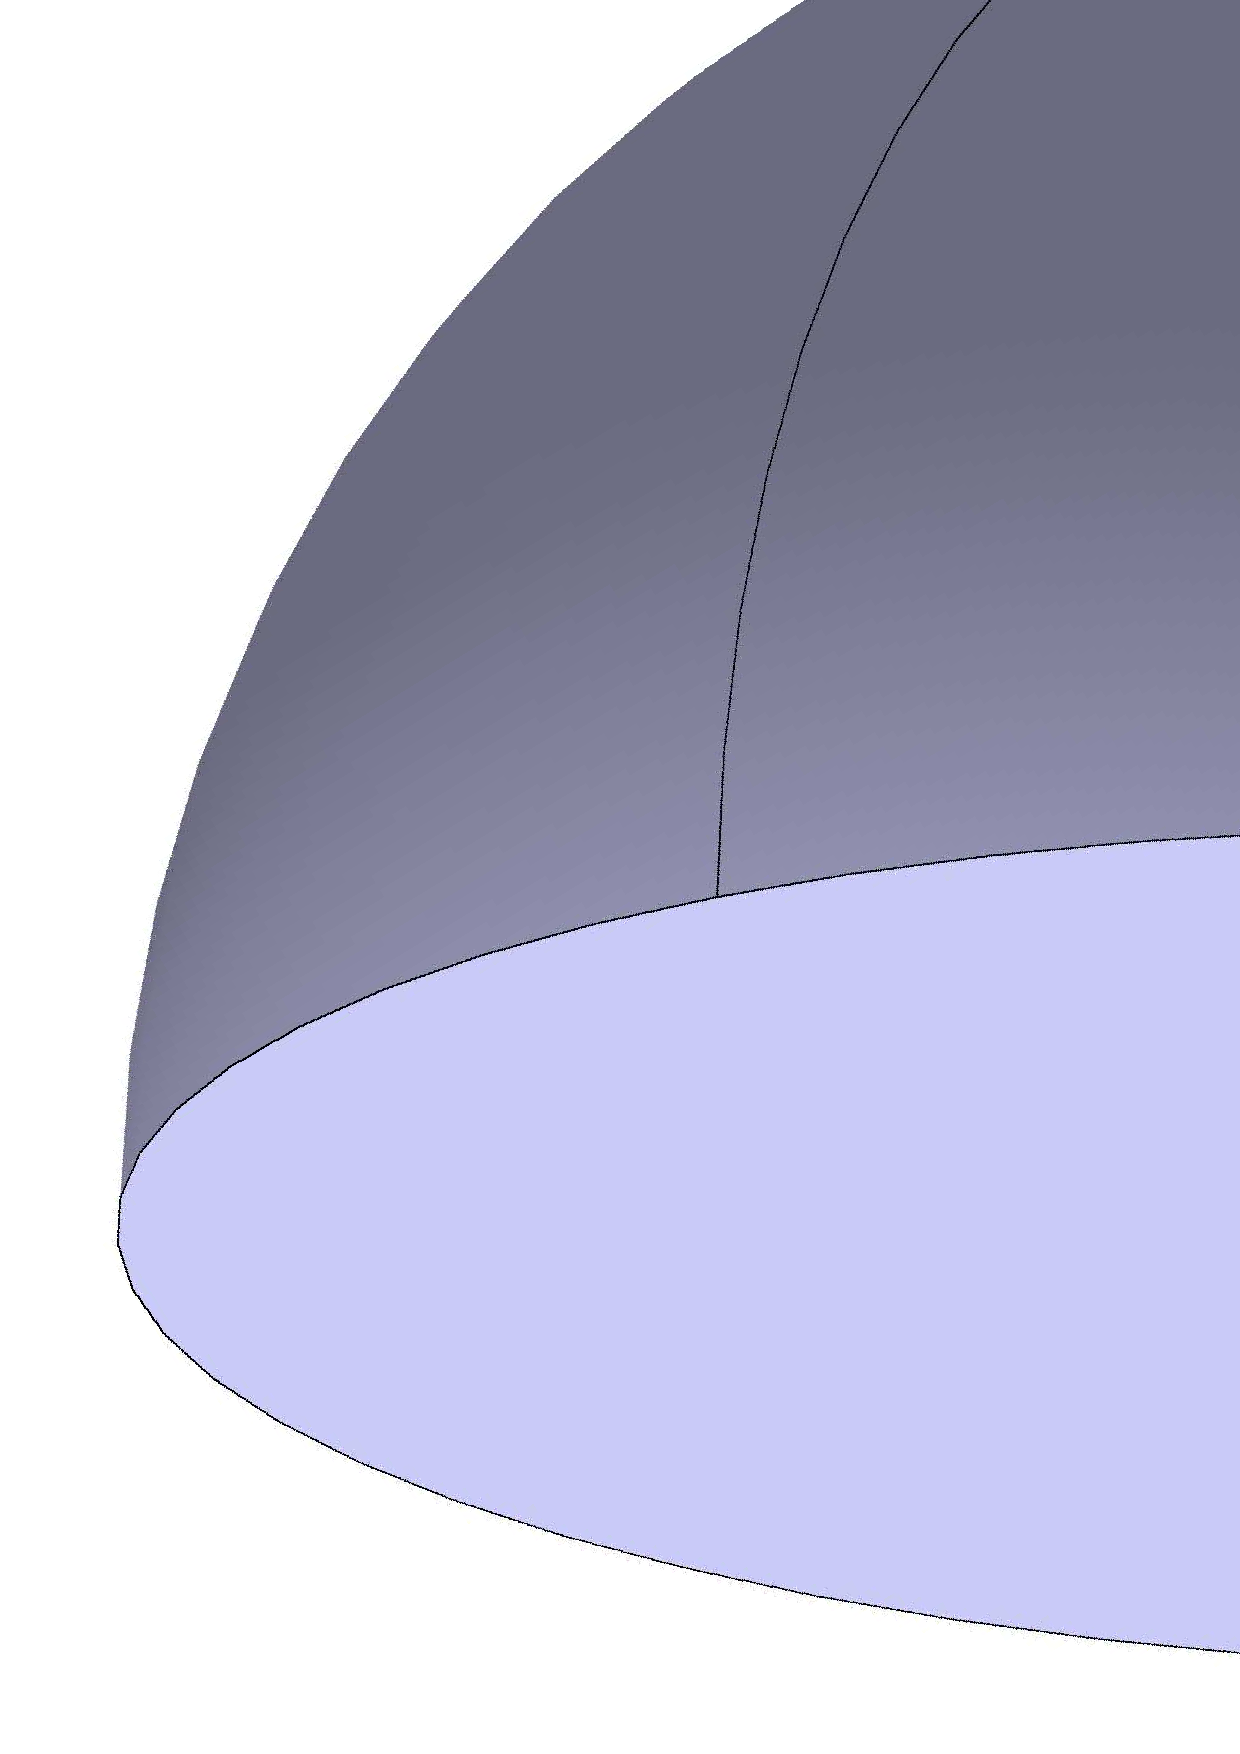
\includegraphics[width=1in]{Figures/blue/Sphere3d.png}  & & 
\includegraphics[width=1in]{Figures/blue/FullSpheroid3d.png} & & 
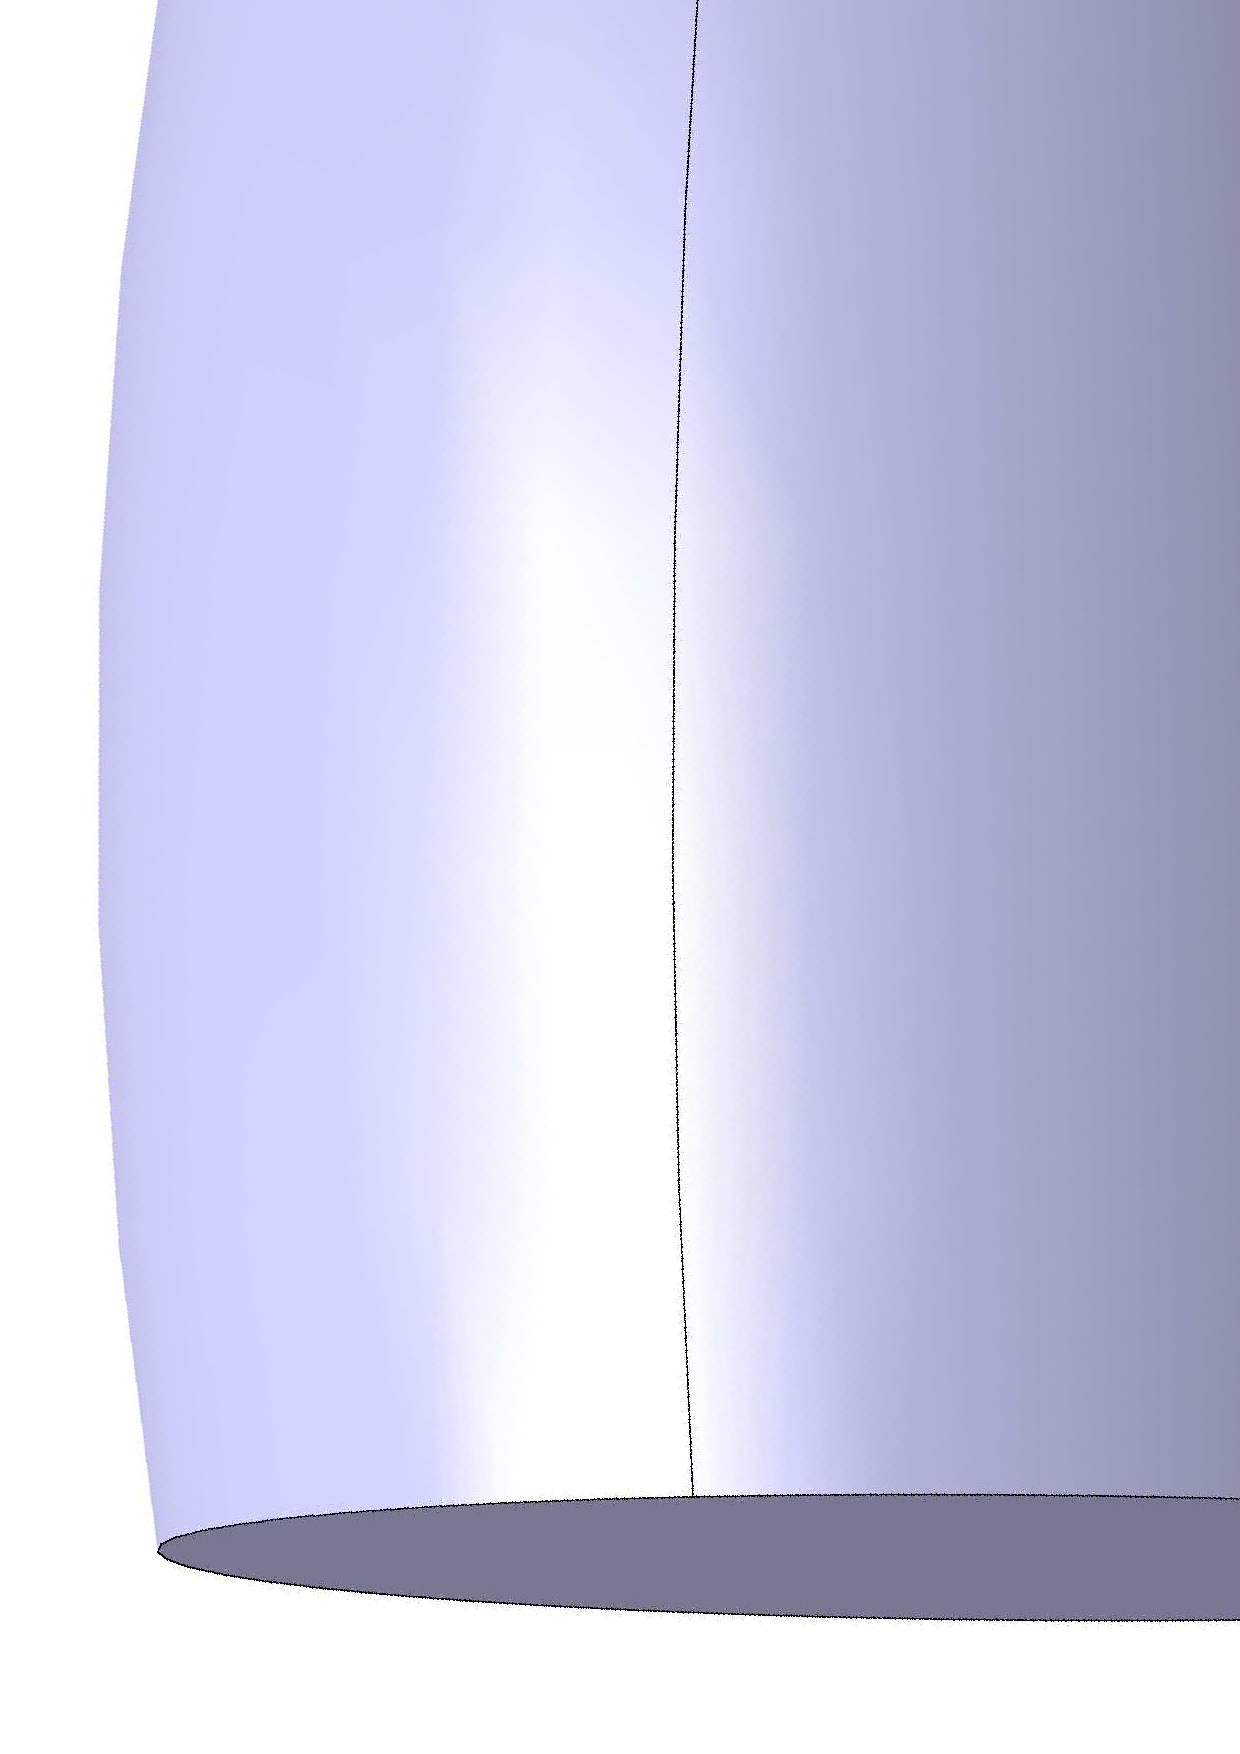
\includegraphics[width=1in]{Figures/blue/Spheroid3d.png} & & 
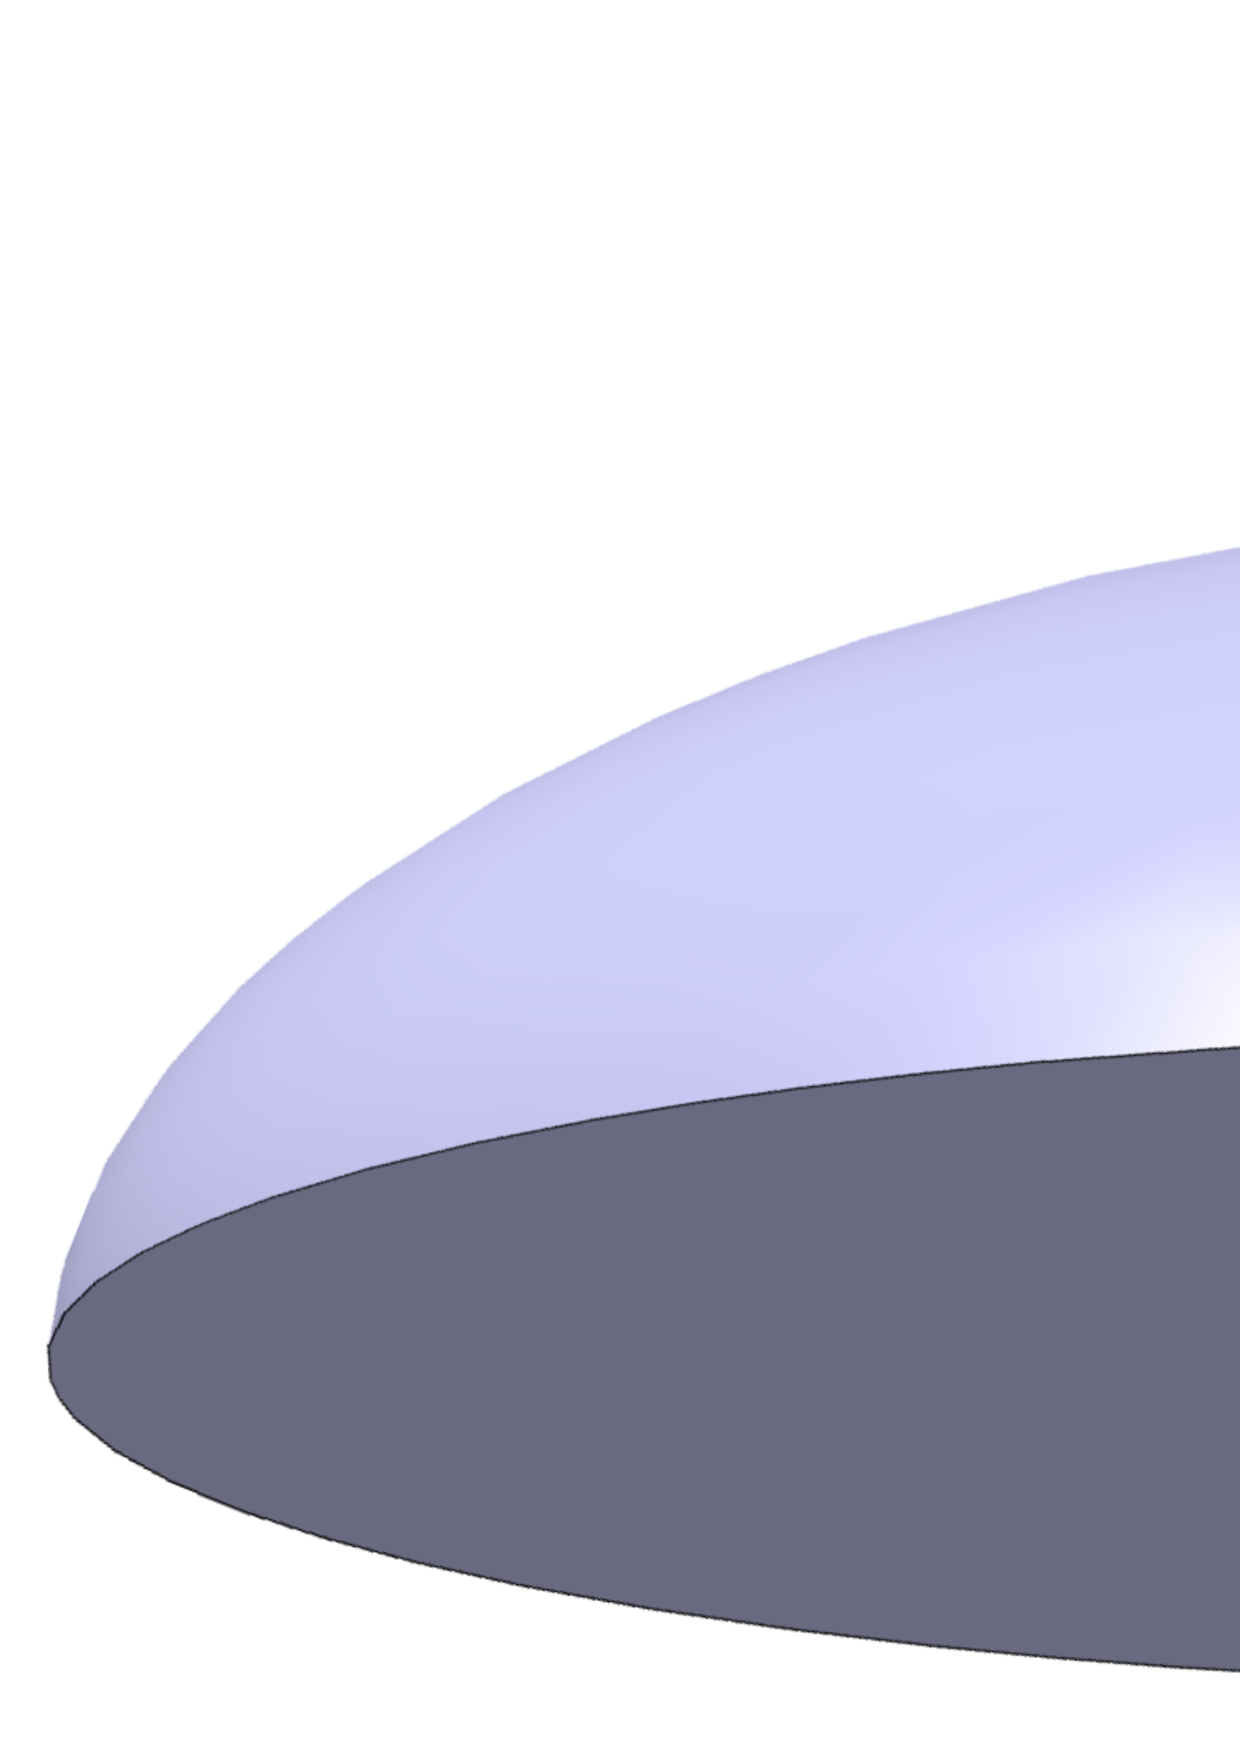
\includegraphics[width=1in]{Figures/blue/HemiEllipsoid3d.png}\\
\hline
Ripple1, \SecRef{Ripple1} &  & Ripple2, \SecRef{Ripple2}& &   & &  \\
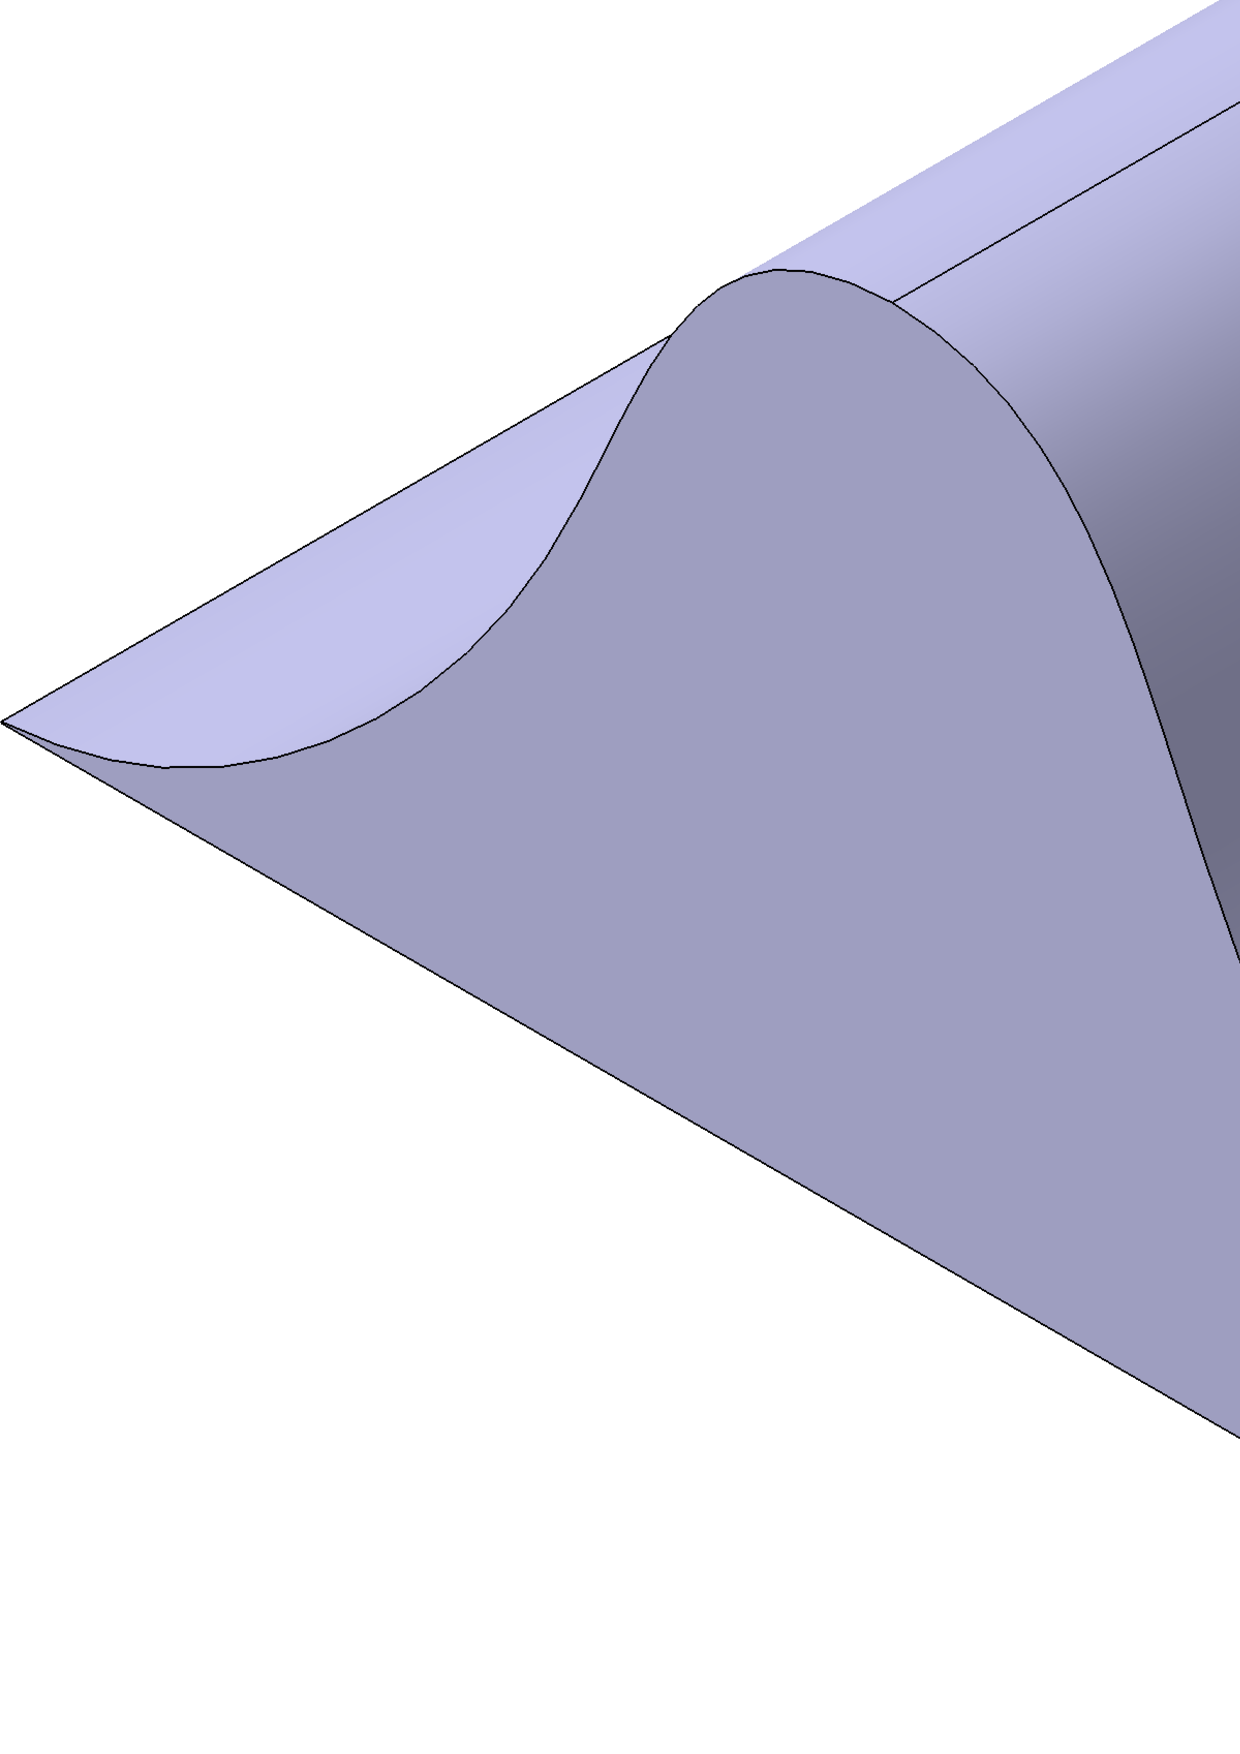
\includegraphics[width=1in]{Figures/blue/Ripple13d.png} & & 
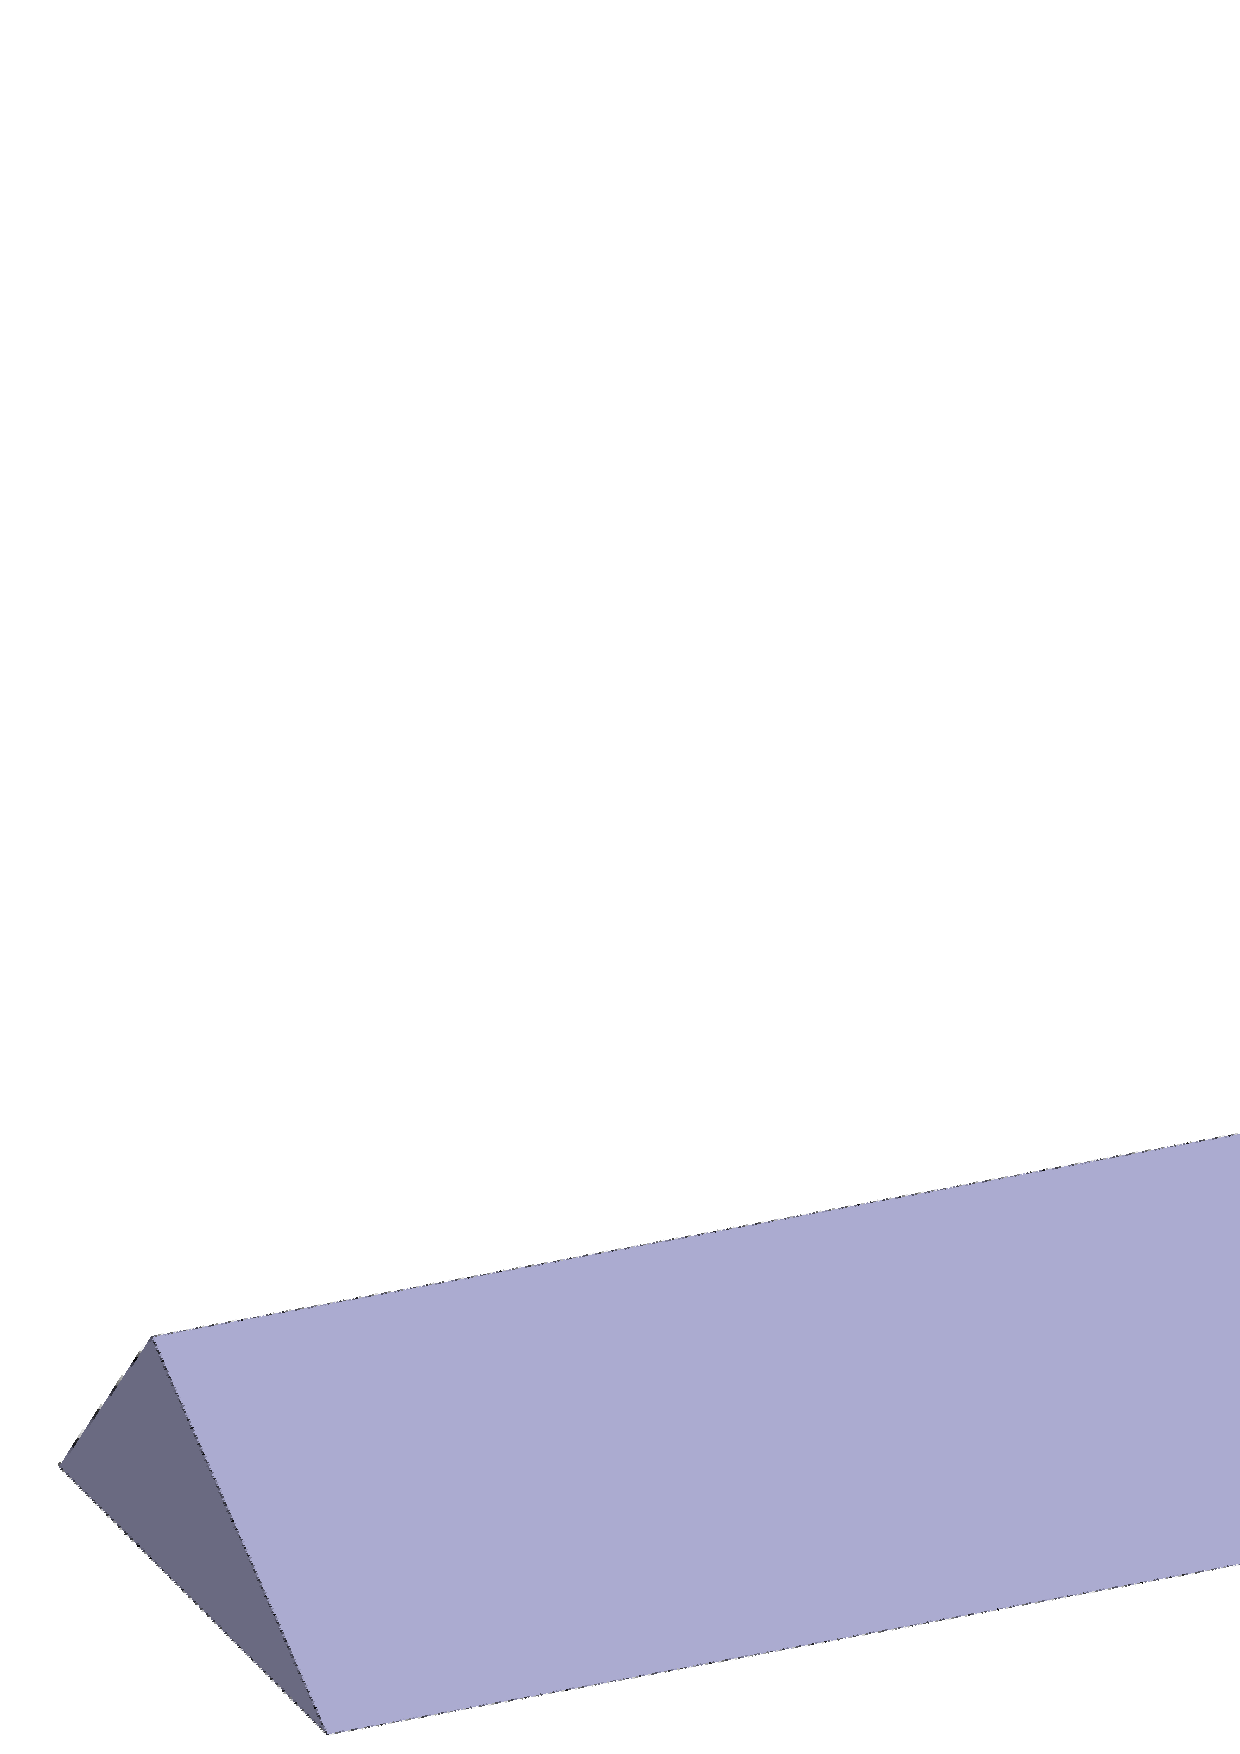
\includegraphics[width=1in]{Figures/blue/Ripple23d.png} & &  & & \\
\hline 
\end{tabulary}
\end{table}

\newpage

%%%%%%%%%%%%%%%%%%%%%%%%%%%%%%%%%%%%%%%%%%%%%%%%%%%%%%%%%%%%%%%%%%%%%%%
\subsection{Distorted Wave Born Approximation} \SecLabel{sect:dwba}

The Born approximation fails when multiple reflections and refractions have to be taken into account at interfaces because of the presence of underlying layers of materials and the closeness of  the incident angle $\alpha_i$ to the critical angle of total external reflection $\alpha_c$. The first order correction to the scattering theory is the Distorted Wave Born Approximation (DWBA), whereas the Born approximation is the zeroth order. \\
The collective effects between the particles are not considered in this section. They have been described in~\SecRef{sect:interf}.  We also do not take any polarization effects into account. \\

 In the DWBA, the form factor of a particle in a multilayer system is given by

\begin{align}
F_{\rm{DWBA}} (\vect{k}_i,\vect{k}_f, r_z) & = T_i T_f F_{\rm{BA}} (\vect{k}_i-\vect{k}_f) e^{i (k_{i,z}-k_{f,z}) r_z} + R_i T_f F_{\rm{BA}}(\vect{\widetilde{k}}_i-\vect{k}_f) e^{i(-k_{i,z}-k_{f,z})r_z}
 \nonumber \\
  &+ T_i R_f F_{\rm{BA}}(\vect{k}_i-\vect{\widetilde{k}}_f)e^{i(k_{i,z}+k_{f,z})r_z} + R_iR_fF_{\rm{BA}} (\vect{\widetilde{k}}_i-\vect{\widetilde{k}}_f)e^{i(-k_{i,z}+k_{f,z})r_z} \; , \label{eq:dwbageneral}
\end{align}
where $F_{\rm{BA}}$ is the expression of the form factor in the Born approximation, $r_z$ is the $z$-coordinate of the particle's position (measured from the bottom of the particle), $\vect{k}_i=(k_{i,x}, k_{i,y}, k_{i,z})$ $\vect{k}_f=(k_{f,x}, k_{f,y}, k_{f,z})$ are the incident and scattered wave vectors in air, respectively \cite{RaSS95}. With a tilde (\~{}), these wavevectors components are evaluated in the multilayer system (the refractive indices of the different constituting materials have to be taken into account). 
$T_i$, $T_f$, $R_i$, $R_f$ are the transmission and reflection coefficients for the incident wave (index $i$) or the scattered one (index $f$). These coefficients can be calculated using the Parratt formalism \cite{Par54} or the matrix method \cite{BoWo99}. $\vect{k}_i-\vect{k}_f$ is equal to the scattering vector $\vect{q}$ and the $z$-axis is pointing upwards.\\

\ImportantPoint{Remark:}{The particles cannot sit in between layers. At most they can be sitting on any inner interfaces.}

\vspace{18pt}

In the followings, the DWBA will be illustrated for two different layouts of particles: 
\begin{itemize}
\item particles deposited on a substrate,
\item particles buried in a layer on a substrate.
\end{itemize}

\ImportantPoint{Remark:}{In \BornAgain\ there is no limitation to the number of layers composing the sample.}

%%%%%%%%%%%%%%%%%%%%%%%%%%%%%%%%%%%%%%
\subsubsection{Particles deposited on a substrate}
%Substrate modified Born approximation
In this configuration, the particles are sitting on top of a substrate layer, in the air as shown in fig.~\ref{fig:SchemDWBA}. In the DWBA the expression of a form factor becomes 
\begin{align}
F_{\rm{DWBA}}(q_{\parallel}, k_{i,z}, k_{f,z}) &= F_{\rm{BA}}(q_{\parallel}, k_{i,z}-k_{f,z})+ R_i F_{\rm{BA}}(q_{\parallel}, -k_{i,z}-k_{f,z}) \nonumber \\
&+ R_f F_{\rm{BA}}(q_{\parallel}, k_{i,z}+k_{f,z}) + R_i R_f F_{\rm{BA}}(q_{\parallel},-k_{i,z}+k_{f,z}), \label{eq:dwbaair}
\end{align}
where $q_{\parallel}$ is the component of the scattering beam in the plane of the interface ($\vect{q}=\vect{k}_i-\vect{k}_f$), $k_{i,z}$ and $k_{f,z}$ are the z-component of the incident and scattered beam, respectively. $R_i$, $R_f$ are the reflection coefficients in incidence and reflection. They are defined as\\ $R=\dfrac{k_z+\sqrt{n_s^2k_0^2-|k_{\parallel}|^2}}{k_z-\sqrt{n_s^2 k_0^2-|k_{\parallel}|^2}}$, where $n_s=1-\delta_s +i \beta_s$ is the refractive index of the substrate, $k_0$ is the wavelength in vacuum ($2\pi /\lambda$), $k_z$ and $k_{\parallel}$ are the $z$-component and the in-plane component of $\vect{k}_i$ or $\vect{k}_f$. \\

\ImportantPoint{Remark:}{If the particles are sitting on a multilayered system, the expression of the form factor in the DWBA is obtained by replacing the Fresnel coefficient by the corresponding coefficients of the underlying layers \cite{Par54,BoWo99}.}

\vspace{18pt}

Figure~\ref{fig:SchemDWBA} illustrates the four scattering processes for a supported particle, taken into account in the DWBA. The first term of eq.~\ref{eq:dwbaair}  corresponds to the Born approximation. Each term of $F_{\rm{DWBA}}$ is weighted by a Fresnel coefficient. 

\begin{figure}[ht]
\begin{center}
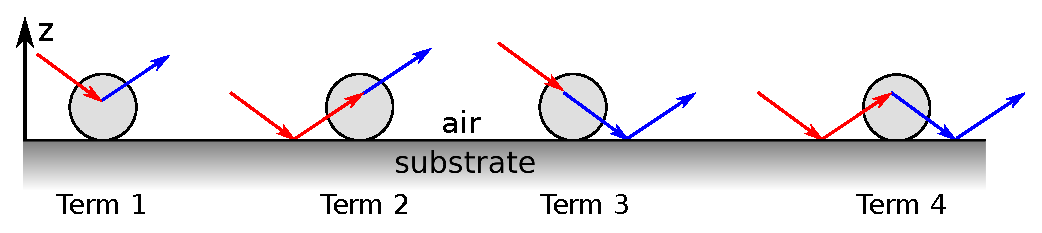
\includegraphics[width=\textwidth]{Figures/drawing/drawingDWBA.eps}
\end{center}
\caption{Schematic views of the different terms appearing in the expression of the form factor under DWBA for particles sitting on a substrate layer.}
\label{fig:SchemDWBA}
\end{figure}


Script~\ref{lst:badwba} illustrates the difference between BA and DWBA in \BornAgain\ when generating the sample.  We consider the simple case of:
\begin{itemize}
\item one kind of particles' shape,
\item no interference between the particles,
\item in the DWBA, a sample made of a layer of substrate on which are deposited the particles,
\item in the BA, a sample composed of the particles in air.
\end{itemize} 

Figure~\ref{fig:spheroidbadwba} shows the intensity contourplot generated using this script with truncated spheroids as particles.

\newpage


\begin{lstlisting}[language=python, style=eclipseboxed,numbers=none,nolol,caption={\Code{Python} script to generate a sample using Born (BA) or Distorted Wave Born Approximation (DWBA). The difference between BA and DWBA in this simple case is the absence or presence of a substrate layer in the sample.},label={lst:badwba}]
def get_sample():
    """
    Build and return the sample to calculate form factor of 
    truncated spheroid in Born or Distorted Wave Born Approximation.
    """
    # defining materials
    m_ambience = HomogeneousMaterial("Air", 0.0, 0.0)
    m_substrate = HomogeneousMaterial("Substrate", 6e-6, 2e-8)
    m_particle = HomogeneousMaterial("Particle", 6e-4, 2e-8)

    # collection of particles
    ff= FormFactorTruncatedSpheroid(7.5*nanometer, 9.0*nanometer, 1.2)
    particleshape = Particle(m_particle, ff)
    particle_layout = ParticleLayout()
    particle_layout.addParticle(particleshape, 0.0, 1.0)

    # interferences
    interference = InterferenceFunctionNone()
    particle_layout.addInterferenceFunction(interference)

    # assembling the sample
    air_layer = Layer(m_ambience)
    air_layer.addLayout(particle_layout)
    substrate_layer = Layer(m_substrate, 0)

    multi_layer = MultiLayer()
    multi_layer.addLayer(air_layer)
    # Comment the following line out for Born Approximation
    multi_layer.addLayer(substrate_layer)
    return multi_layer
\end{lstlisting}


\begin{figure}[ht]
\hfill
\subfigure[Born Approximation]{\includegraphics[angle=-90,width=6cm]{Figures/gisasmap/ffspheroidBA.pdf}}
\hfill
\subfigure[DWB Approximation]{\includegraphics[angle=-90,width=6cm]{Figures/gisasmap/ffspheroidDWBA.pdf}}
\hfill
\caption{Intensity map of TruncatedSpheroid form factor in BA and DWBA computing using script~\ref{lst:badwba} for the sample.}
\label{fig:spheroidbadwba}
\end{figure}

\FloatBarrier 

\ImportantPoint{Remark:}{In \BornAgain, the DWBA is implemented automatically when assembling the sample with more layers than only the air layer (for example, for particles are sitting on a substrate).}

\subsubsection{Buried particles} 

The system considered in this section consists of particles encapsulated in a layer, which is sitting on a substrate (see fig.~\ref{fig:SchemDWBAburied}). In this case the form factor in the DWBA is given by

\begin{align}
F_{\rm{DWBA}}(q_{\parallel}, k_{i,z}, k_{f,z}) &= T_i T_f F_{\rm{BA}}(q_{\parallel}, k_{i,z}-k_{f,z})e^{i(k_{i,z}-k_{f,z})d}+ R_i T_f F_{\rm{BA}}(q_{\parallel}, -k_{i,z}-k_{f,z})e^{i(-k_{i,z}-k_{f,z})d} \nonumber \\
&+ R_f T_i F_{\rm{BA}}(q_{\parallel}, k_{i,z}+k_{f,z}) e^{i(k_{i,z}+k_{f,z})d}+ R_f R_iF_{\rm{BA}}(q_{\parallel},-k_{i,z}+k_{f,z})e^{i(-k_{i,z}+k_{f,z})d}, \label{eq:dwbaburied}
\end{align}

\begin{equation*}
R_j =\frac{t^{j}_{0,1}r^{j}_{1,2}\exp(2ik_{j,z}t)}{1+r^{j}_{0,1}r^{j}_{1,2}\exp(2ik_{j,z}t)}, \quad T_j=\frac{t^{j}_{0,1}}{1+r^{j}_{0,1}r^{j}_{1,2}\exp(2ik_{j,z}t)}, j=i,f 
\end{equation*}
where $q_{\parallel}$ is the component of the scattering beam in the plane of the interface, $k_{i,z}$ and $k_{f,z}$ are the z-component of the incident and scattered beams, respectively.  $d$ is the depth at which the particles are sitting in the layer. Note that this value is given relative to the top of this layer and it is not the coordinate in the absolute referential (linked with the full sample) and it is measured up to the bottom of the particle. $t$ is the thickness of the intermediate layer containing the particles. $R_{i,f}$ and $T_{i,f}$  are the reflection  and transmission coefficients in incidence and reflection (they can be calculated using Parratt or matrix formalism). $r^j_{0,1}$, $r^j_{1,2}$ $t^j_{0,1}$ are the reflection and transmission coefficients between layers; the indices are related to different boundaries with 0: air, 1: intermediate layer and 2: substrate layer and the superscript $j$ is associated with the incident or scattered beams:
\begin{equation*}
r^j_{n,n+1}=\frac{k_{j,z,n}-k_{j,z,n+1}}{k_{j,z,n}-k_{j,z,n+1}}, \qquad t^j_{n,n+1}= \frac{2k_{j,z,n}}{k_{j,z,n}-k_{j,z,n+1}}, \quad n=0,1, \quad j=i,f,
\end{equation*}
where index $n$ is related to the layers, $z$ to the vertical component, and $j$ to the beams (incident and outgoing).

\begin{figure}[ht]
\begin{center}
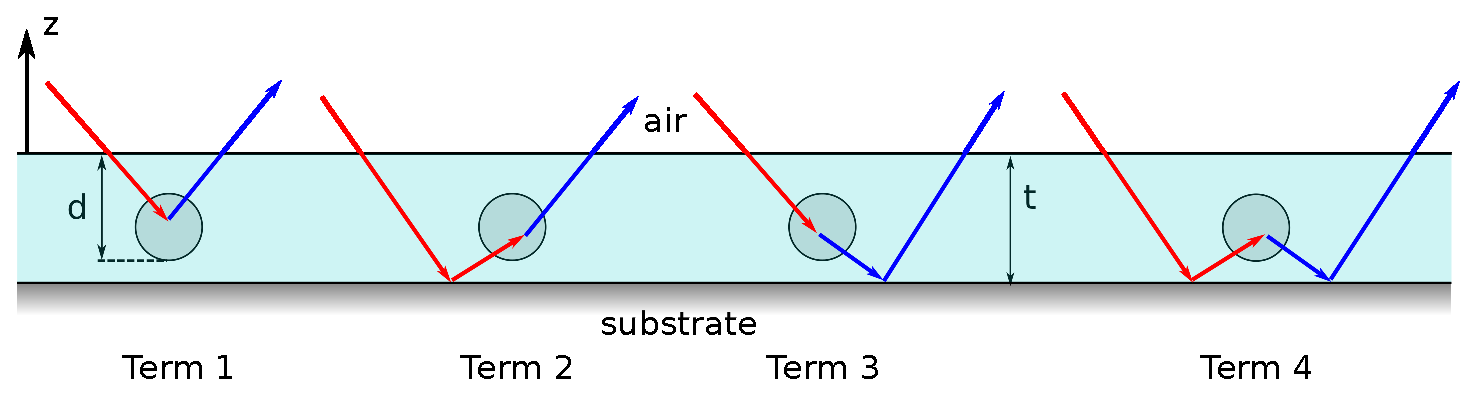
\includegraphics[width=\textwidth]{Figures/drawing/drawingDWBAburied.eps}
\end{center}
\caption{Schematic views of the different terms appearing in the expression of the form factor under the DWBA for buried particles.}
\label{fig:SchemDWBAburied}
\end{figure}



Figure~\ref{fig:dwbaburied} shows a typical example of the output intensity scattered from a sample made of 3 layers: air, substrate, and in between, spherical particles embedded in the middle of a 30~nm-thick layer. This figure had been generated using listing~\ref{lst:dwbaburied}.

\begin{lstlisting}[language=python, style=eclipseboxed,numbers=none,nolol,caption={\Code{Python} script to generate a sample where spherical particles are embedded in the middle of a layer on a substrate.},label={lst:dwbaburied}]
def get_sample():
    """
    Build and return the sample with buried spheres in DWBA.
    """
    # defining materials
    m_ambience = HomogeneousMaterial("Air", 0.0, 0.0)
    m_interm_layer = HomogeneousMaterial("IntermLayer",3.45e-6, 5.24e-9)
    m_substrate = HomogeneousMaterial("Substrate", 7.43e-6, 1.72e-7)
    m_particle = HomogeneousMaterial("Particle", 0.0, 0.0)

    # collection of particles 
    ff = FormFactorFullSphere(10.2*nanometer)
    particleshape = Particle(m_particle, ff)
    particle_layout = ParticleLayout()
    particle_layout.addParticle(particleshape,25.2,1.0)

    # interferences 
    interference = InterferenceFunctionNone()
    particle_layout.addInterferenceFunction(interference)

    # assembling the sample 
    air_layer = Layer(m_ambience)
    intermediate_layer = Layer(m_interm_layer, 30.*nanometer)
    intermediate_layer.addLayout(particle_layout)
    substrate_layer = Layer(m_substrate, 0)
   
    multi_layer = MultiLayer()
    multi_layer.addLayer(air_layer)
    multi_layer.addLayer(intermediate_layer)
    multi_layer.addLayer(substrate_layer)
    return multi_layer
\end{lstlisting}


\begin{figure}[ht]
\centering
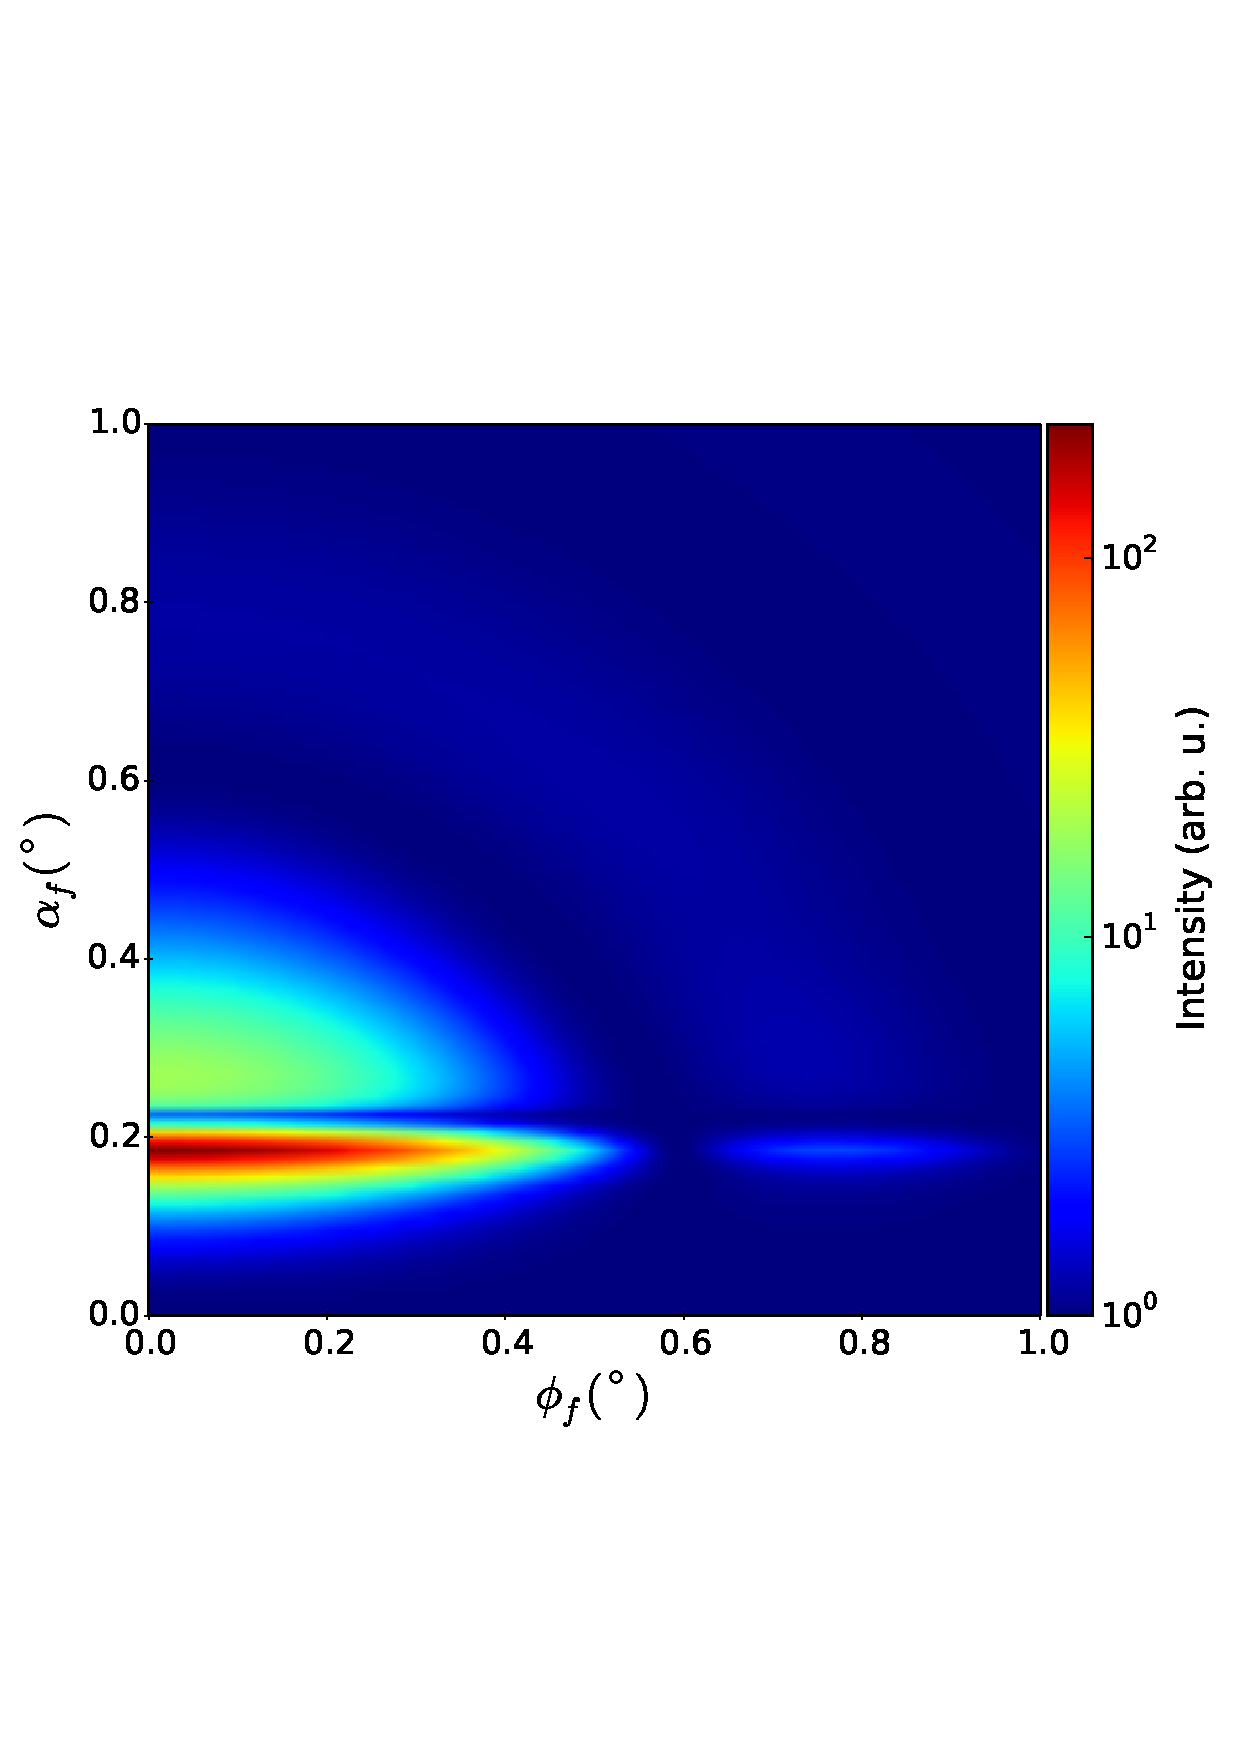
\includegraphics[width=0.6\textwidth]{Figures/gisasmap/figIntBuriedPart.pdf}
\caption{Map of intensity scattered from a sample made of spherical particles embedded in the middle of a 30~nm-thick layer on a substrate (see Script~\ref{lst:dwbaburied} for details about the sample).}
\label{fig:dwbaburied}
\end{figure}

\newpage

\ImportantPoint{Remark:}{For layers different from the air layer, the top interface is considered as the reference level to position the encapsulated particles. For example, spheres positioned at depth $d$ (positive) are located at a distance $d$ from the top of the layer up to the bottom of these particles. This convention is different for the top air layer, where particles sitting at the interface with an underlying layer (\textit{i.e.} the bottom of the air layer) are located at depth 0 (see fig.~\ref{fig:depthpartBA}).}


\begin{figure}[ht]
\centering
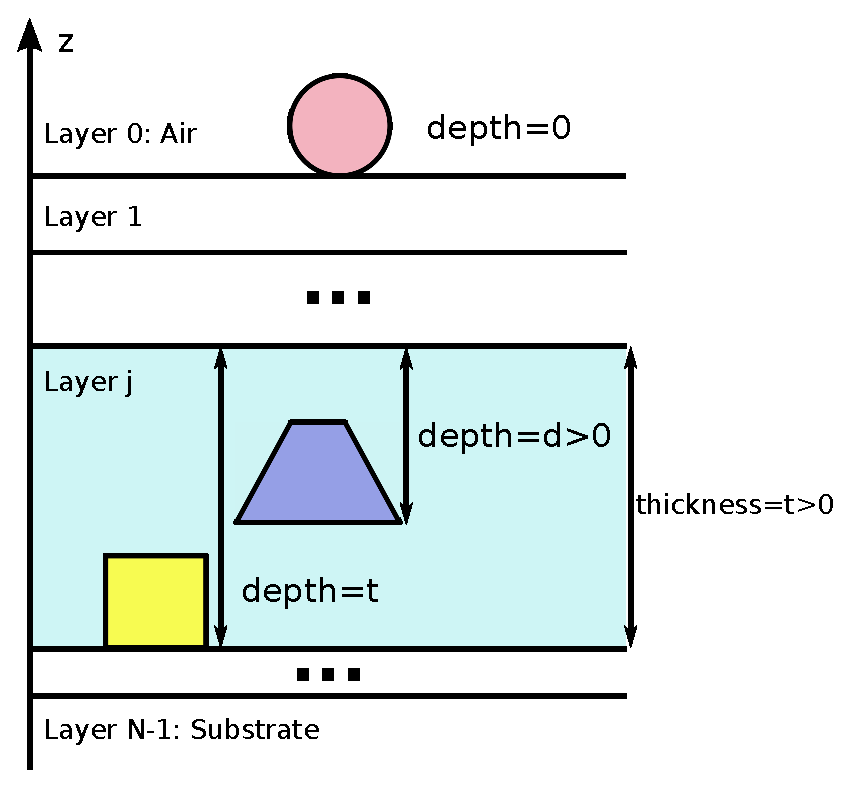
\includegraphics[width=0.5\textwidth]{Figures/drawing/drawingDepthParticle.eps}
\caption{Illustration of the convention about \Code{depth} used in \BornAgain\ to encapsulate particles in layers.}
\label{fig:depthpartBA}
\end{figure}


\newpage
%%%%%%%%%%%%%%%%%%%%%%%%%%%%%%%%%%%%%%%%%%%%%%%%%%%%%%%%%%%%%%%%%%%%%%%%%%%%%%%%
\section{More complicated particles' shapes} 
%%%%%%%%%%%%%%%%%%%%%%%%%%%%%%%%%%%%%%%%%%%%%%%%%%%%%%%%%%%%%%%%%%%%%%%%%%%%%%%%

\BornAgain\ also offers the possibility to simulate more complicated shapes of particles by combining those listed in Table~\ref{tab:formfactors}. 

\subsection{Core-shell particles} \label{subsec:CoreShell}
 To generate a core-shell particle, the combination is performed using the following command:\\
\Code{ParticleCoreShell(shell\_particle, core\_particle, relative\_core\_position)},\\
where \Code{shell\_particle} and \Code{core\_particle} are the outer and inner parts of the core-shell particle, respectively. They refer to one of the form factors defined previously and to an associated material. For example, for the outer part,\\ \Code{shell\_particle=Particle(material\_shell, outer\_form\_factor)},\\ where \Code{material\_shell} is the material of the shell and \Code{outer\_form\_factor} is the shape of the outer part (cf. listing~\ref{lst:cshellsample}). \\ \Code{relative\_core\_position} defines the position of the inner shape with respect to the outer one; it is defined with respect to the centre of the base of the particular form factor. An example in fig.~\ref{fig:coreshell} shows a core shell particle made of a box for the outer part and of a shifted pyramidal shape for the inner one.\\

Figure~\ref{fig:FFCoreShellBA} displays the output intensity scattered in the Born Approximation using the code listed in~\ref{lst:cshellsample} to generate the core-shell particle. 

\begin{figure}[ht]
\hfill
\subfigure[Side view]{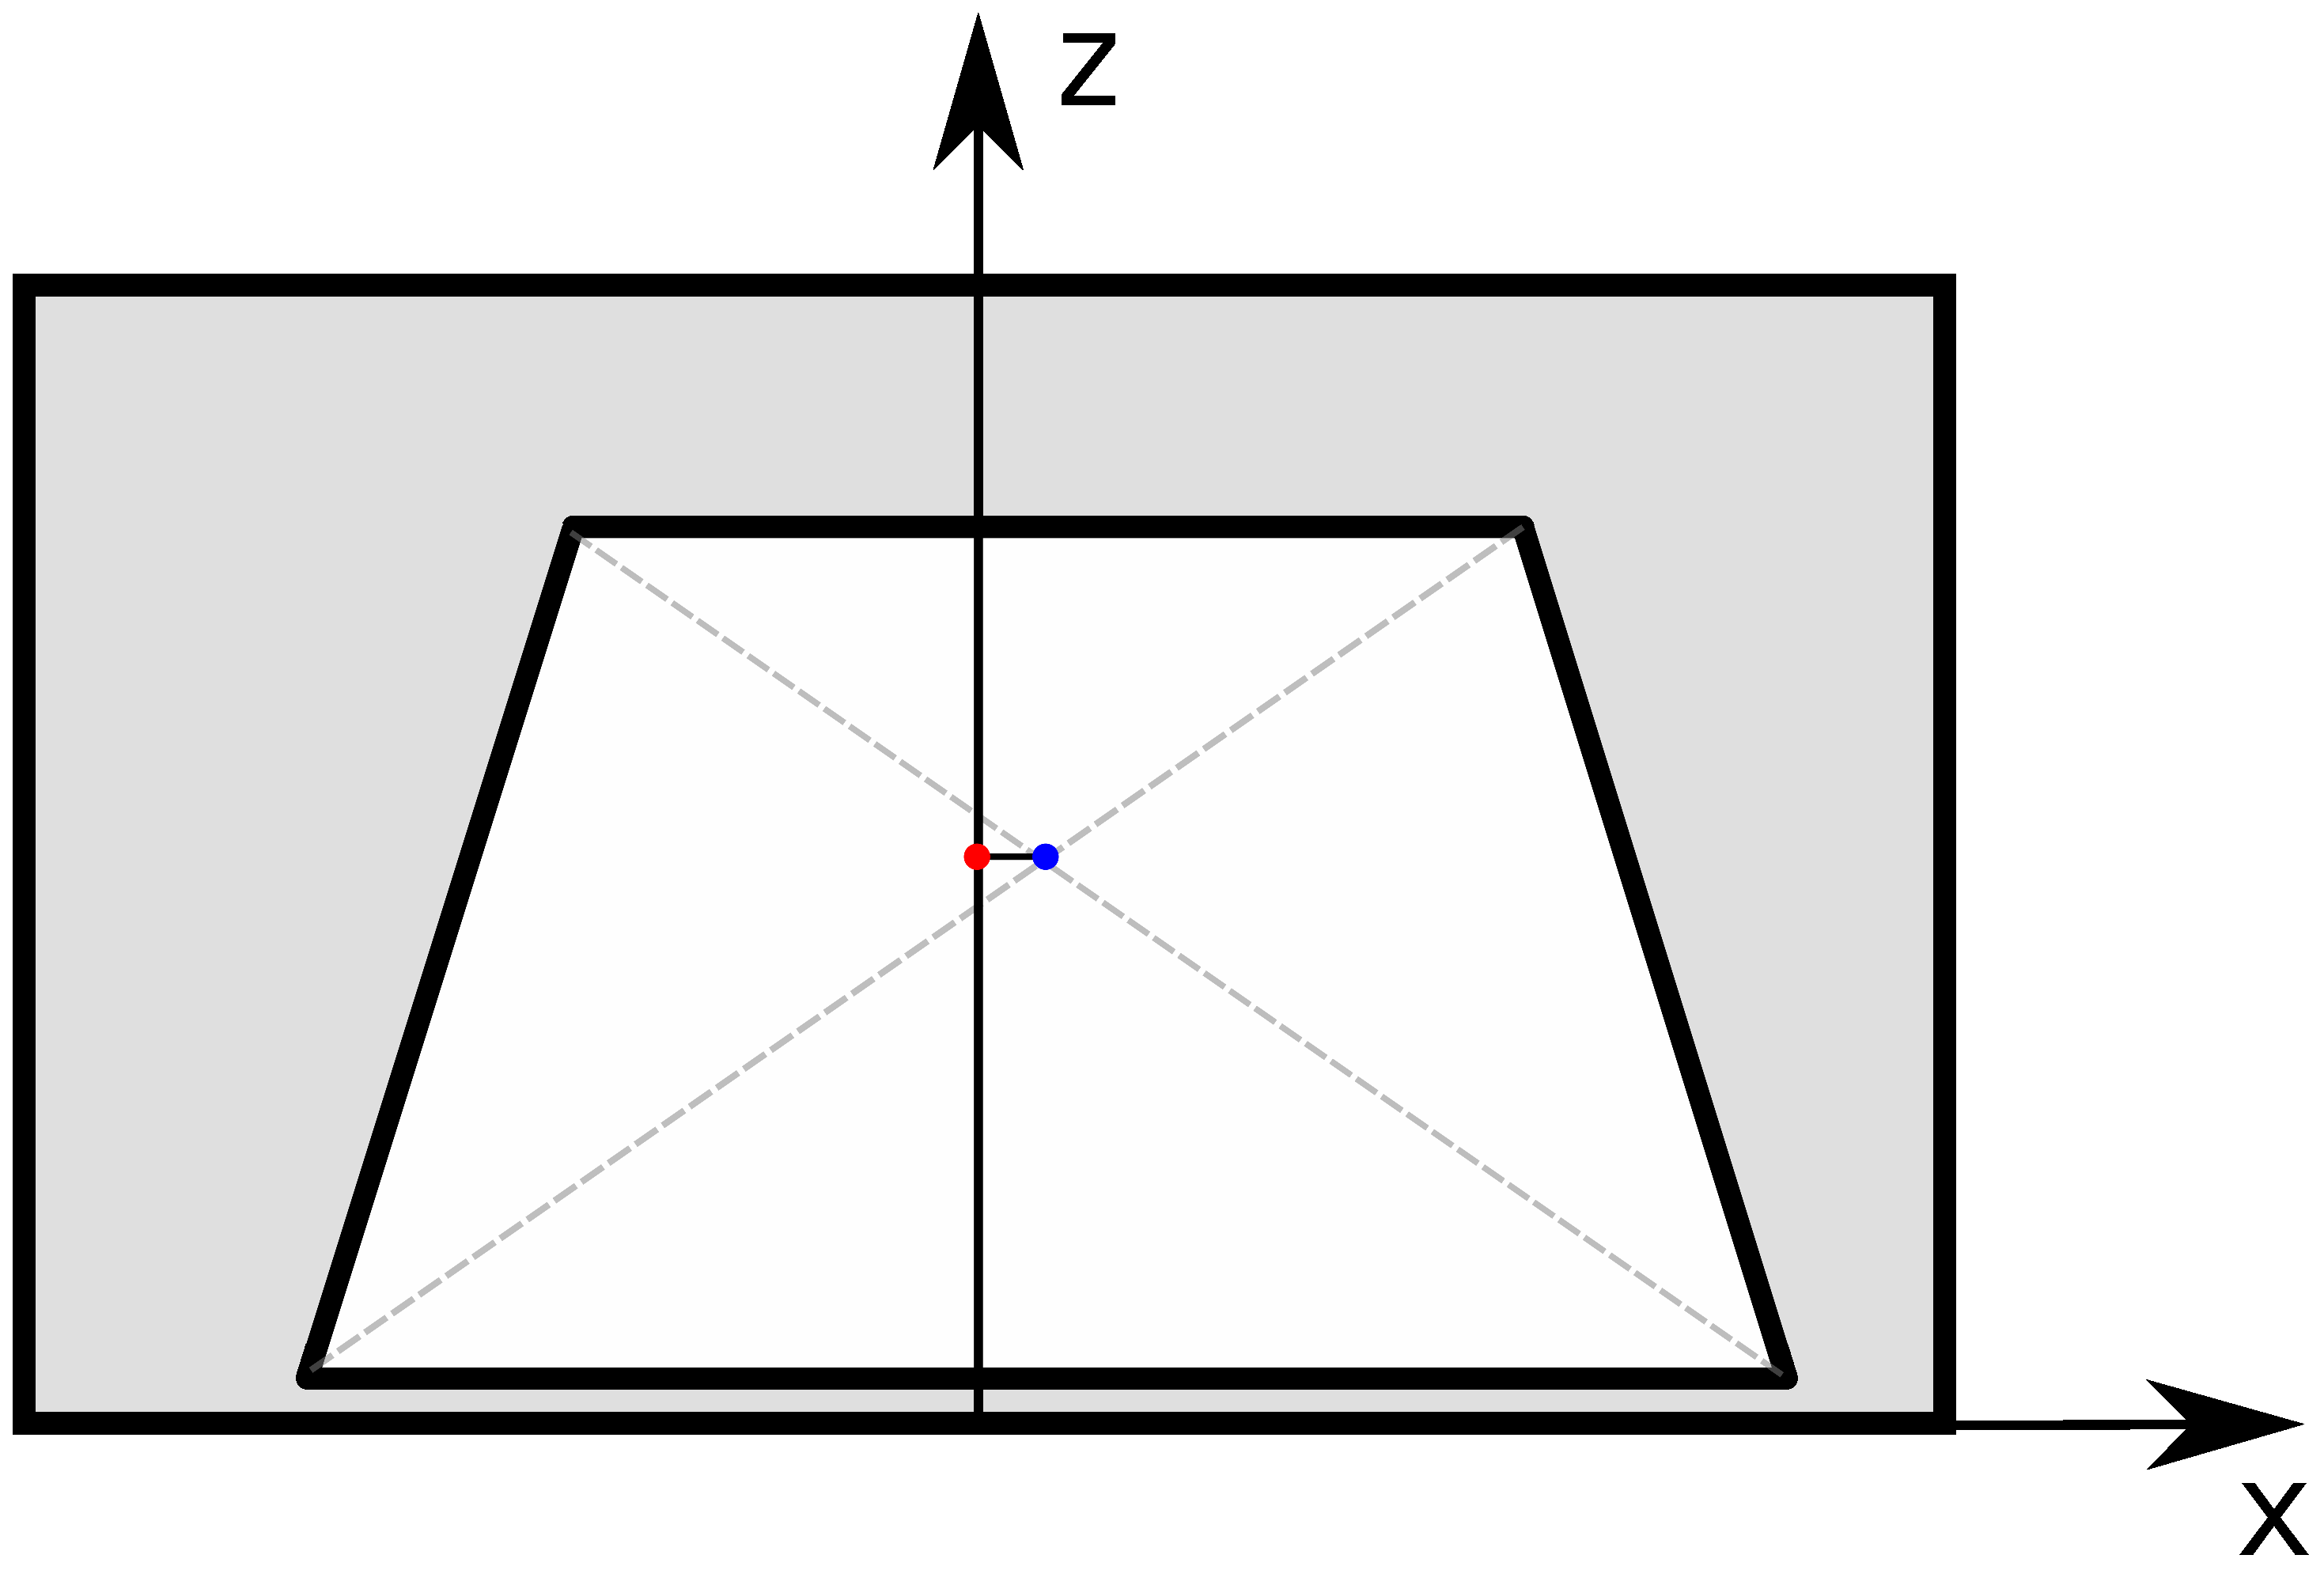
\includegraphics[width=5cm]{Figures/cuts/CoreShellParallPyrxz.eps}}
\hfill
\subfigure[Top view]{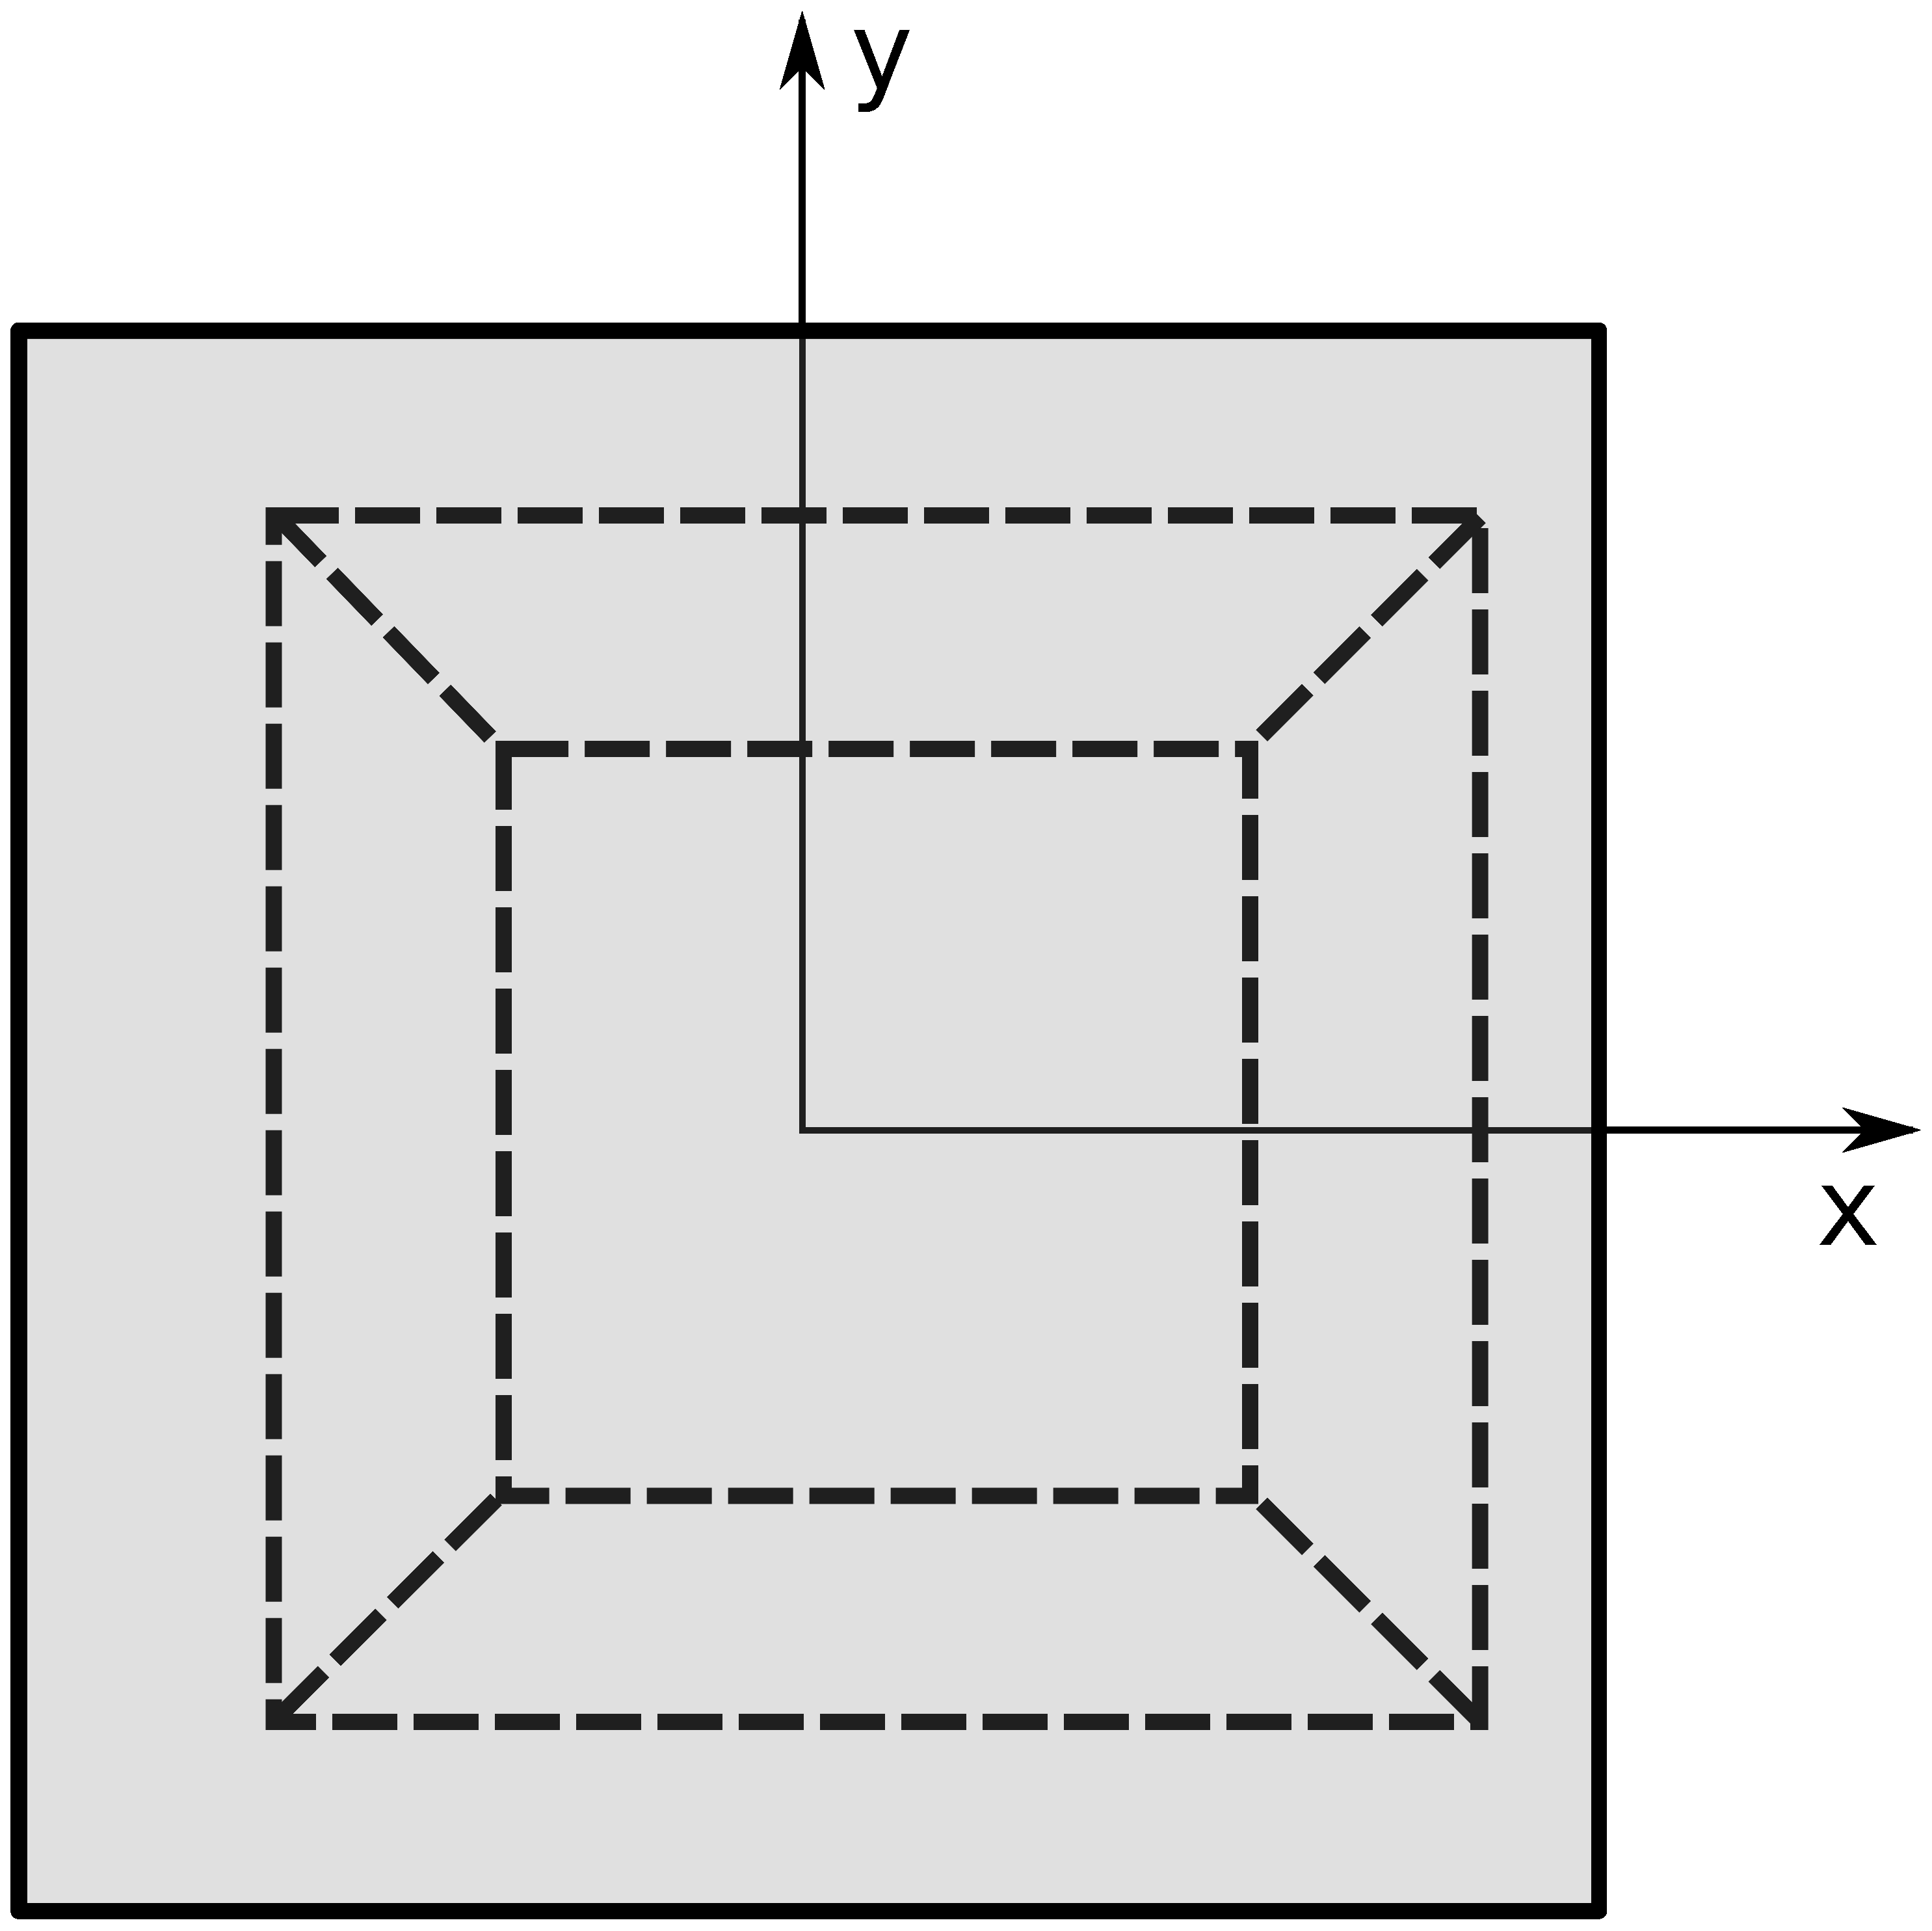
\includegraphics[width=5cm]{Figures/cuts/CoreShellParallPyrxy.eps}}
\hfill
\caption{Example of a core-shell particle composed of a box with a pyramidal  inset. The relative core shell position is marked by the positions of the centres of the bases. }
\label{fig:coreshell}
\end{figure}

\newpage


\begin{lstlisting}[language=python,
  style=eclipseboxed,numbers=none,nolol,caption={\Code{Python} script
    to create a core-shell particle made of a box with a pyramidal shifted inset.},label={lst:cshellsample}]
    outer_ff = FormFactorBox(16.0*nanometer, 16.0*nanometer, 8.0*nanometer) 
    inner_ff = FormFactorPyramid(12.0*nanometer, 7.0*nanometer, 60.0*degree)
    shell_particle = Particle(m_shell, outer_ff)
    core_particle = Particle(m_core, inner_ff)
    core_position = kvector_t(1.5, 0.0, 0.0)

    particle = ParticleCoreShell(shell_particle, core_particle, core_position)
\end{lstlisting}

\begin{figure}[ht]
\begin{center}
\includegraphics[angle=-90,width=0.6\textwidth]{Figures/gisasmap/CoreShellParallPyr.pdf}
\end{center}
\caption{Intensity map of a core-shell form factor in Born Approximation using  \Code{FormFactorBox(16*nanometer, 16*nanometer, 8*nanometer)} and \Code{FormFactorPyramid(12*nanometer, 7*nanometer, 60*degree)} for the outer and inner shells, respectively. The core particle is shifted by 1.5~nm in the $x$-direction with respect to the centre of the outer shell. The sample used to generate the particle is listed in~\ref{lst:cshellsample}.  There is no substrate and no interference between the particles.}
\label{fig:FFCoreShellBA}
\end{figure}

\subsection{Rotation of particles}

The particles can be rotated in a different direction by using one of
the following transformations: \Code{CreateRotateX($\theta$),
  CreateRotateY($\theta$), CreateRotateZ($\theta$)}, where capital X, Y, Z mark rotations
around the associated axis and $\theta$ is the
angle of rotation from this axis. For example, the following \Code{Python}\ script shows how to rotate a pyramid by $45^{\circ}$ around
the $z$-axis:\\

\begin{lstlisting}[language=python, style=eclipseboxed,numbers=none,nolol]
    pyramid_ff = FormFactorPyramid(10*nanometer, 5*nanometer, deg2rad(54.73 ) )
    pyramid = Particle(m_particle, pyramid_ff)
    angle_around_z = 45.*degree
    transform = Transform3D.createRotateZ(angle_around_z)
    particle_layout = ParticleLayout()
    particle_layout.addParticle(pyramid, transform) 
\end{lstlisting}

\subsection{Polydispersity}

%%%%%%%%%%%%%%%%%%%%%%%%%%%%%%%%%%%%%%%%%%%%%%%%%%%%%%%%%%%%%%%%%%%%%%%%%%%%%%%%
\section{Material layers}
%%%%%%%%%%%%%%%%%%%%%%%%%%%%%%%%%%%%%%%%%%%%%%%%%%%%%%%%%%%%%%%%%%%%%%%%%%%%%%%%
\subsection{Roughness}
\section{Polarisation}
To be completed 

\newpage
\chapter{Fitting}

%     Minuit Library:
%         Migrad Algorithm ("Minuit", "Migrad"),
%         Simplex Algorithm ("Minuit", "Simplex")
%         Minimize Algorithm ("Minuit", "Minimize")
%         Scan Algorithm ("Minuit", "Scan")
%         Seek Algorithm ("Minuit", "Seek")
%     Fumili Library:
%         Fumili Algorithm
%     Minuit2 Library:
%         Migrad Algorithm ("Minuit2", "Migrad")
%         Simplex Algorithm ("Minuit2", "Simplex")
%         Minimize Algorithm ("Minuit2", "Minimize")
%         Scan Algorithm ("Minuit2", "Scan")
%         Fumili2 Algorithm ("Minuit2", "Fumili2")
%     GSL Library: (Only available if GSL and MathMore are avaiable too)
%         Fletcher-Reeves Conjugate Gradient Algorithm ("GSLMultiMin", "conjugatefr")
%         Polak-Ribiere Conjugate Gradient Algorithm ("GSLMultiMin", "conjugatepr")
%         BFGS Conjugate Gradient Algorithm ("GSLMultiMin", "bfgs2")
%         Levenberg-Marquardt Algorithm ("GSLMultiFit", "")
%         Simulated Annealing Algorithm ("GSLSimAn", "")

In addition to the simulation of grazing incidence
x-ray and neutron scattering by
multilayered samples, BornAgain also offers the option to
fit a selection of simulated sample parameters to experimental data.  This aspect
of the software is discussed in this chapter.

%%%%%%%%%%%%%%%%%%%%%%%%%%%%%%%%%%%%%%%%%%%%%%%%%%%%%%
\section{Short description of fitting theory}

These features of BornAgain deal with estimating the optimum parameters
in the simulation by minimizing the difference ($\chi^2$) between theory and experimental data.\\

\textbf{From Minuit user's guide}: Minuit is usually used to find the ``best'' values of a set of
parameters, where ``best'' is defined as those values which minimize a
given function, FCN. The width of the function minimum in some
neighbourhood of the minimum, gives information about the uncertainty
in the best parameter values. An important feature of Minuit is that
it offers several tools to analyze the parameter errors.



\noindent \smallpencil \colorbox{Lightgray}{\parbox{\dimexpr\linewidth-8\fboxsep}
{\underline{Theory}: Users wanting to find out more about minimization (also called
maximization or optimization methods) are referred to \ldots.}}\\

%The conjugate gradient and BFGS methods are described in detail in the following book,
%    R. Fletcher, Practical Methods of Optimization (Second Edition) Wiley (1987), ISBN 0471915475. 
%A brief description of multidimensional minimization algorithms and more recent references can be found in,
%    C.W. Ueberhuber, Numerical Computation (Volume 2), Chapter 14, Section 4.4 Minimization Methods, p. 325–335, Springer (1997), ISBN 3-540-62057-5
%The simplex algorithm is described in the following paper,
%    J.A. Nelder and R. Mead, A simplex method for function minimization, Computer Journal vol. 7 (1965), 308–313. 
% W. T. Eadie, D. Drijard, F. James, M. Roos, and B. Sadouletm
% Statistical methods in experimental physics, North-Holland 1971

Local minimum, multiple minima

%\url{http://seal.web.cern.ch/seal/MathLibs/Minuit2/html/}

%\url{http://seal.web.cern.ch/seal/documents/minuit/mntutorial.pdf}

%\url{http://root.cern.ch/root/html/MATH_MINUIT2_Index.html}

A detailed tutorial of Minuit software can be downloaded at the
following address \url{http://seal.web.cern.ch/seal/documents/minuit/mnusersguide.pdf}.
%\cite{MinuitRoot}.

Local or global minimization
%%%%%%%%%%%%%%%%%%%%%%%%%%%%%%%%%%%%%%%%%%%%%%%%%%%%%%
\section{Implementation in BornAgain}
BornAgain fitting features include...\\
Different geometries, number of fit parameters, variety of minimizers\\
and minimization strategies.\\

Minimizer belongs to MinimizerFactory (interacts with Root)

Variable parameters: customize lists, inputs required, default values

Methods: implemented list, possibility to add your own.

Set/create minimizer : name + algorithm + option (part of Minimizer
factory). The minimizers can be chosen from the following list:

FitSuite: m\_minimizer, m\_is\_last\_iteration

\textbf{Questions}
\begin{itemize}
\item Is it possible to fit on the particle kind (cylinder or prism or
\ldots)?
\item Fit using several experimental runs?
\item Number of degrees of freedom?
\item Weighted fits?
\item Errorbars, epsilon for standard error
\item Normalisation of the data (in order to be compared)
\item Constraints between parameters
\item Quick fit option
\item Possible exponential decrease of the form factor
\item fit of 1D plots?
\end{itemize}
%To run tests: python TestFit.py\\
%List of tests\\
%TestFit01 - Two parameter fit using variety of minimizers. Geometry: cylinders in the air.\\
%TestFit02 - Fitting using sample builder\\


Class TestFittingModule1: 
\begin{itemize}
\item mp\_real\_data (experimental data), 
\item mp\_simulated\_data,
\item mp\_simulation, 
\item mp\_sample, 
\item mp\_fitsuite: \texttt{addSimulationAndRealdData}: link a given set of experimental data with a
  particular set of simulated data in order to proceed to a fit. It is
  therefore possible to generate a batch of different numerical
  samples to test different configurations in order to obtain the best
  fit by playing with the number of layers or the shape of particles
  (different form factors). What about \texttt{chi2\_module} by default?
\end{itemize} 

\texttt{attachObserver} uses
\texttt{FitSuiteObserverFactory::CreatePrintObserver()} or
\texttt{FitSuiteObserverFactory::CreateDrawObserver()} or
\texttt{FitSuiteObserverFactory::CreateTreeObserver()}.


%runFit()

%%%%%%%%%%%%%%%%%%%%%%%%%%%%%%%%%%%%%%%
\subsubsection{General procedure to fit / for fitting}

Format of input (experimental data) - requirements (structure,
normalisation, values...)
Experimental data can be entered by importing it from ASCII files created by other applications.
%Therefore the number of layers cannot be used as a fitting parameter

A fit is run for a fixed value of \textbf{the number of layers
  constituting the sample}, the \textbf{input beam wavelength}.

Input = matrix of intensity as function of ?

Generation of the numerical model (cf other examples or detailed
description or only script given and description of main steps)

\textbf{Structure of fitting module in BornAgain.}


\textbf{Structure of Fit folder (sources *.cpp):}
\begin{itemize}
\item FitObject.cpp
\item FitSuiteObjects.cpp		
\item MinimizerFactory.cpp
\item ROOTMinimizer.cpp
\item FitParameter.cpp		
\item FitSuiteParameters.cpp		
\item MinimizerScan.cpp		
\item ROOTMinimizerHelper.cpp
\item FitParameterLinked.cpp		
\item FitSuitePrintObserver.cpp	
\item MinimizerTest.cpp
\item FitSuite.cpp			
\item FitSuiteStrategies.cpp		
\item ROOTGSLNLSMinimizer.cpp
\item FitSuiteFunctions.cpp		
\item IFitSuiteStrategy.cpp
\item ROOTGSLSimAnMinimizer.cpp
\end{itemize}

\textbf{Structure of Fit folder (headers *.h):}
\begin{itemize}
\item AttFitting.h		
\item FitSuite.h		
\item FitSuiteStrategies.h	
\item MinimizerTest.h		
\item ROOTMinimizerHelper.h
\item AttLimits.h		
\item FitSuiteFunctions.h	
\item IFitSuiteStrategy.h	
\item ROOTGSLNLSMinimizer.h
\item FitObject.h		
\item FitSuiteObjects.h	
\item IMinimizer.h		
\item ROOTGSLSimAnMinimizer.h
\item FitParameter.h		
\item FitSuiteParameters.h	
\item MinimizerFactory.h	
\item ROOTMinimizer.h
\item FitParameterLinked.h	
\item FitSuitePrintObserver.h	
\item MinimizerScan.h		
\item ROOTMinimizerFunction.h
\end{itemize}

\myparagraph{\underline{Choice of parameters to be fitted}}
In principle, every parameter used in the construction of the sample
can be used as a fit parameter. For example

\begin{table}[h]
\centering
\begin{tabular}{|@{}l||l@{}|}
\hline
\textbf{Particles} &  dimensions: height, radius, length, width, \\
                             &  half side length, thickness, \textbf{index of refraction} 
                             height\_aspect\_ratio, \textbf{orientation?} \\
& (depending on the shape) \\
& inteference (density, proportion, width, distance,\\
& probability,
dispersion radius) \\
\hline
\textbf{Lattice} & \\
\hline
\textbf{Layers} & roughness, thickness, \textbf{index of refraction} \\
\hline
\textbf{Beam} & intensity \\
\hline
\textbf{Detector} & \\
\hline
\end{tabular}
\label{table:fitting_parameters}
\caption{List of parameters that can be defined as fitting parameters.}
\end{table}

The heights of different particles can be associated to two different
fitting parameters and optimized / minimized separately.


m\_cylinder\_ratio, m\_cylinder\_height
m\_prism3\_half\_side, m\_prism3\_height
                          
  *Normalizer/scale
  *Normalizer/shift

  *SampleBuilder/particle\_probability1
  *SampleBuilder/particle\_radius1
  *SampleBuilder/dispersion\_radius1
  *SampleBuilder/height\_aspect\_ratio1

  *SampleBuilder/interf\_distance
  *SampleBuilder/interf\_width

 *SampleBuilder/height\_aspect\_ratio
 
   */lattice\_length\_a 
   */lattice\_length\_c   
   */nanoparticle\_radius",     
   */sigma\_nanoparticle\_radius
   */meso\_height       
   */meso\_radius  
   */sigma\_meso\_height
   */sigma\_meso\_radius
   */sigma\_lattice\_length\_a
   */surface\_filling\_ratio
   */roughness

 
In BornAgain, the parameters used for the fit are specified using the
function \texttt{addFitParameter} with the following syntax:

\begin{lstlisting}[language=C++, style=eclipse,numbers=none]
m\_fitSuite->addFitParameter("*height", 4.*Units::nanometer,
0.04*Units::nanometer, AttLimits::lowerLimited(0.01) );

m\_fitSuite->addFitParameter("*radius", 6.*Units::nanometer,
0.06*Units::nanometer, AttLimits::lowerLimited(0.01) );

m\_fitSuite->addFitParameter("*SampleBuilder/m\_cylinder\_height",4*Units::nanometer, 0.01*Units::nanometer,AttLimits::lowerLimited(0.01) );

m\_fitSuite->addFitParameter("*SampleBuilder/m\_cylinder\_radius",
  6*Units::nanometer, 0.01*Units::nanometer, AttLimits::lowerLimited(0.01) );

m\_fitSuite->addFitParameter("*SampleBuilder/m\_prism3\_half\_side", 4*Units::nanometer, 0.01*Units::nanometer,  AttLimits::lowerLimited(0.01) );
\end{lstlisting}

There are two possible syntaxes:
\begin{itemize}
\item First option: \\ \texttt{m\_fitSuite->addFitParameter(name, value, step, attlim, error);},
where \texttt{value}, \texttt{step} and \texttt{error} are double values corresponding to the ... respectively.
\item Second option: \\
\texttt{m\_fitSuite->addFitParameter(name, value, attlim, error);}
\end{itemize}

\texttt{attlim} is , \texttt{name} is ...
By default the input value of \texttt{error} is 0.
 

\texttt{AttLimits} can be
\begin{itemize}
\item fixed(), 
\item lowerLimited(double value), 
\item limited(double min value, double max value).
\end{itemize}
The unit of \texttt{AttLimits} is  identical to the one used to characterize the
parameter.

Number of iterations
Interrupt fit
Procedure: initially choose a small number of fitting parameters

\textbf{ Software Scatter :The program allows to automatically fit large number of data files such as files from timeresolved
studies. A requirement is that subsequent scattering curves do not differ too much, so
that the fitted values of the first curve can be used as starting parameters for a fit to the next
curve. Before starting a fit series, choose the first data file and perform a fit so that the
parameter values are set to an optimal start value. The first/last point, qmin/max and Imin for
the fit will apply to all data sets.}

Background noise, intensity threshold.


%%%%%%%%%%%%%%%%%%%%%%%%%%%%%%%%%%%%%%%
\subsubsection{Fitting methods implemented}

\textbf{Is there any default method implemented?}
Different minimizers from Root library can be used in BornAgain. They are listed in
Table~\ref{table:fit_minimizers}. Users can also add their own by
implementing their definition in the \texttt{Catalogue} contained in
program \texttt{MinimizerFactory}.
Minuit user's manual describes which minimizer to use in order to best
fit our data\ldots  \cite{MinuitRoot}.

\begin{table}[h]
\centering
\begin{tabular}{@{}ll@{}}
\hline
\hline
\textbf{Minimizer name - Library} & \textbf{Algorithm} \\
\hline
%Test & \\
%Scan & \\%[-3pt] 
Minuit & Migrad, Simplex, Combined, Scan\\
Minuit2 & Migrad, Simplex, Combined, Scan, Fumili \\
Fumili & \\
GSLMultiMin & ConjugateFR, ConjugatePR, BFGS, BFGS2, SteepestDescent \\
GSLMultiFit & \\
GSLSimAn & \\ %Simulatded annealing algorithm
Genetic &  \\ %TMVA Toolkit for Multivariate Data Analysis with ROOT 
\hline
\hline
\end{tabular}
\label{table:fit_minimizers}
\caption{List of fitting minimizers implemented in BornAgain.}
\end{table}




Minuit2, originally developed in the SEAL project, is now distributed
within ROOT. The classes have been moved inside the namespace
ROOT::Minuit2. 

Minuit is conceived as a tool to find the minumum value of a
multi-parameter function and analyze the shape of the function around
the minimum. The principal application is foreseen for statistical
analysis, working on chisquare or log-likelihood functions, to compute
the best-fit parameter values and uncertainties, including
correlations between the parameters. It is especially suite to handle
difficult problems, including those which may requier guidance in
order to find the correct solution.

Minuit2, optional package in the ROOT framework, is a numerical minimization computer program
originally written in C++ programming language. The program searches for minima in a user-defined function with
respect to one or more parameters using several different methods as
specified by the user. 
%%%%%%%%%%%%%%%%%%%%%%%%%%%%%%%%%%%%%%%
\subsubsection{Outputs}
log file, how to interpret the data, how to save the estimated parameters.
Customize using \texttt{Observer}.
See FitGISAXS, IsGISAXS, Fish.
%%%%%%%%%%%%%%%%%%%%%%%%%%%%%%%%%%%%%%%%%%%%%%%%%%%%%%
\section{Examples}
in C++ or Python?
TestPyFit: testfit01.py, testfit02.py
FitSuite

Observer

Screenshot after running the program
Graph?
Simulation
Real data


Difference between TestFit and TestPyFit

Different steps to follow - order of execution

%%%%%%%%%%%%%%%%%%%%%
\myparagraph{\underline{First step:} Initializing the simulation}

 definition of the detector's
  parameters \texttt{setDetectorParameters} and the beam's parameters
  \texttt{setBeamParameters}

%%%%%%%%%%%%%%%%%%%%%
\myparagraph{\underline{Generating the sample}}

Layers, particles, 

%%%%%%%%%%%%%%%%%%%%%
\myparagraph{\underline{Choice of parameters to be fitted}}

choice of parameters
  to be used for minimization \texttt{addFitParameter}. 

%%%%%%%%%%%%%%%%%%%%%
\myparagraph{\underline{Running the simulation / the fit}}

Normalisation ?

Output = two-dimensional matrix.

How to run the fit: using the function \texttt{fit}



\begin{lstlisting}[caption={Python script of fitting example},
  label=script_exfit1,captionpos=b,escapeinside={@}{@} ,language=python,style=eclipse, numbers= none,frame = leftline ,
      framerule = 2mm ,
      rulecolor = \color{lightgrey},
      breaklines = true]
# In this test we are using simple geometry: cylinders without interference in
# air layer with two parameters (radius and height of cylinders), describing
# the sample. Our "real" data is 2D intensity map obtained from the simulation of
# the same geometry with fixed values height = 5nm and radius = 5nm.
# Then we run our minimization consequently using different minimization engines,
# with height=4nm, radius=6nm as starting fit parameter values.
import sys
import os
import numpy
import time

sys.path.append(os.path.abspath(
                os.path.join(os.path.split(__file__)[0],
                '..', '..', '..', 'lib')))

from libBornAgainCore import *
from libBornAgainFit import *

# sample parameters we are going to find
cylinder_height = 5*nanometer
cylinder_radius = 5*nanometer

# minimizer name and type of minimization algorithm
Minimizers = [ 
    ("Minuit2","Migrad"), 
    ("Minuit2","Fumili"), 
    ("GSLMultiMin","BFGS"),
    ("GSLMultiMin","SteepestDescent"),
    ("GSLMultiFit",""),
#    ("GSLSimAn","")
]

# -----------------------------------------------------------------------------
# run several minimization rounds using different minimizers
# -----------------------------------------------------------------------------
def runTest():
    #print "**********************************************************************"
    #print "*  Starting  TestFit01                                               *"
    #print "**********************************************************************"
    nTest=0
    status = "OK"
    for m in Minimizers:
        minimizer_name = m[0]
        minimizer_algorithm = m[1]
        print "Minimizer {0:-2d}   {1:}({2:})".format(nTest, minimizer_name, minimizer_algorithm)
        result_ok = run_fitting(minimizer_name, minimizer_algorithm)
        nTest+=1
        if not result_ok: status = "FAILED"

    return "TestFit01", "Two parameters fit using variety of minimizers.", status

# -----------------------------------------------------------------------------
# run fitting specified minimizer
# -----------------------------------------------------------------------------
def run_fitting(minimizer_name, minimizer_algorithm):
    sample = buildSample()
    simulation = createSimulation()
    simulation.setSample(sample)

    # creating real data, which is simply results of our simulation with default values
    simulation.runSimulation()
    real_data = simulation.getOutputDataClone()

    # setting fit suite
    fitSuite = FitSuite()
    fitSuite.setMinimizer( MinimizerFactory.createMinimizer(minimizer_name, minimizer_algorithm) )
    fitSuite.addFitParameter("*height", 4.*nanometer, 0.04*nanometer, AttLimits.lowerLimited(0.01) )
    fitSuite.addFitParameter("*radius", 6.*nanometer, 0.06*nanometer, AttLimits.lowerLimited(0.01) )
    fitSuite.addSimulationAndRealData(simulation, real_data)

    # run fit
    start_time = time.time()
    fitSuite.runFit()
    real_time = time.time() - start_time

    height_found = fitSuite.getMinimizer().getValueOfVariableAtMinimum(0)
    height_diff = abs(height_found - cylinder_height)/cylinder_height
    radius_found = fitSuite.getMinimizer().getValueOfVariableAtMinimum(1)
    radius_diff = abs(radius_found - cylinder_radius)/cylinder_radius

    print "            RealTime : {0:.3f} sec".format(real_time)
    print "            NCalls   : {0:<5d}".format(fitSuite.getNCalls())
    print '            par1     : {0:.4f} ({1:.3g}) '.format(height_found, height_diff)
    print '            par2     : {0:.4f} ({1:.3g}) '.format(radius_found, radius_diff)

    diff = 1.0e-02
    isSuccess = True
    if( (height_diff > diff) or (radius_diff > diff) ) : isSuccess=False
    return isSuccess

# -----------------------------------------------------------------------------
# create cylinders in the air
# -----------------------------------------------------------------------------
def buildSample():
    cylinder_ff = FormFactorCylinder(cylinder_height, cylinder_radius)
    n_particle = complex(1.0-6e-4, 2e-8)
    cylinder = Particle(n_particle, cylinder_ff)
    interference = InterferenceFunctionNone()

    particle_decoration = ParticleDecoration()
    particle_decoration.addParticle(cylinder)
    particle_decoration.addInterferenceFunction(interference)

    mAmbience = MaterialManager.getHomogeneousMaterial("Air", 1.0, 0.0 )
    air_layer = Layer(mAmbience)
    air_layer_decorator = LayerDecorator(air_layer, particle_decoration)
    multi_layer = MultiLayer()
    multi_layer.addLayer(air_layer_decorator)

    return multi_layer

def createSimulation():
    simulation = Simulation();
    simulation.setDetectorParameters(100, 0.0*degree, 2.0*degree,100 , 0.0*degree, 2.0*degree);
    simulation.setBeamParameters(1.0*angstrom, -0.2*degree, 0.0*degree);
    simulation.setBeamIntensity(1e10);
    return simulation

#-------------------------------------------------------------
# main()
#-------------------------------------------------------------
if __name__ == '__main__':
    name,description,status = runTest()
    print name,description,status
    if("FAILED" in status) : exit(1)
\end{lstlisting}


Output of functional test: fit module 2 params

TestFittingModule1.cpp with "Minuit2", "Migrad"

\begin{lstlisting}[style=eclipse,numbers=none]
FitSuitePrintObserver::update() -> Info. NCall:0 NStrategy:0 Chi2:6.26500281e+09
Time spend since last call, cpu:0.03 sec, wall time 0.03sec
   # 0 *height                                 4.00000000e+00  lim(0.01,)
   # 1 *radius                                 6.00000000e+00  lim(0.01,)
FitSuitePrintObserver::update() -> Info. NCall:20 NStrategy:0 Chi2:9.29429839e+07
Time spend since last call, cpu:1.27 sec, wall time 4.72sec
   # 0 *height                                 4.51488966e+00  lim(0.01,)
   # 1 *radius                                 4.68705140e+00  lim(0.01,)
FitSuitePrintObserver::update() -> Info. NCall:40 NStrategy:0 Chi2:9.74308159e+05
Time spend since last call, cpu:0.97 sec, wall time 1.05sec
   # 0 *height                                 4.94285364e+00  lim(0.01,)
   # 1 *radius                                 5.07666127e+00  lim(0.01,)
FitSuitePrintObserver::update() -> Info. NCall:60 NStrategy:0 Chi2:7.91181985e+00
Time spend since last call, cpu:1.00 sec, wall time 1.07sec
   # 0 *height                                 4.99977322e+00  lim(0.01,)
   # 1 *radius                                 4.99985065e+00  lim(0.01,)
FitSuitePrintObserver::update() -> Info. NCall:80 NStrategy:0 Chi2:1.01820395e-02
Time spend since last call, cpu:0.98 sec, wall time 1.05sec
   # 0 *height                                 5.00000020e+00  lim(0.01,)
   # 1 *radius                                 5.00000004e+00  lim(0.01,)

FitSuiteObserverPrint::update() -> Info. Printing results

--- FitSuite::printResults --------------------------
 Chi2:1.19798858e-02    chi2.NCall:85  grad.NCall:0,0,0 (neval, ngrad, total)
   # 0 *height                                 4.99999992e+00  lim(0.01,)
   # 1 *radius                                 5.00000004e+00  lim(0.01,)
-----------------------------------------------------
  MinimizerType          : Minuit2
  MinimizerAlgorithm     : Migrad
--- Options -----------------------------------------
  Strategy               : 1
  Tolerance              : 0.01
  MaxFunctionCalls       : 10000
  MaxIterations          : 10000
  Precision              : -1.00
  ErrorDefinition        : 1.00 (1-chi2, 0.5 likelihood)
  ExtraOptions           : 0
--- Status ------------------------------------------ 
  Status                 : 0 'OK, valid minimum'
  IsValidError           : 0 'No detailed error validation'
  CovMatrixStatus        : 3 'full accurate'
  NCalls                 : 85
  MinValue               : 1.01756899e-02
  Edm                    : 4.39332982e-12
--- Variables ---------------------------------------
  NumberOfVariables      : 2 (free), 2 (total) 
  Errors                 : yes, see below
      Npar  Name                                  Value         Error         GlobalCC      
      0    *height                                5.000000e+00  1.109913e-04  1.208255e-01  
      1    *radius                                5.000000e+00  8.941040e-05  1.208255e-01  
--- Correlations-------------------------------------
      1.000000e+00  -1.208255e-01 
      -1.208255e-01 1.000000e+00  
fitting1  : Real Time =   8.33 seconds Cpu Time =   4.58 seconds
\end{lstlisting}



\appendix
\addtocontents{toc}{\protect\setcounter{tocdepth}{1}}
%%%%%%%%%%%%%%%%%%%%%%%%%%%%%%%%%%%%%%%%%%%%%%%%%%%%%%%%%%%%%%%%%%%%%%%%%%%%%%%%
%%
%%   BornAgain:  simulate and fit scattering at grazing incidence
%%
%%   homepage:   http://www.bornagainproject.org
%%
%%   copyright:  Forschungszentrum Jülich GmbH 2015
%%               Software licence does not cover this documentation
%%               For documentation licence, contact the authors
%%   
%%   authors:    Scientific Computing Group at MLZ Garching
%%               C. Durniak, M. Ganeva, G. Pospelov, W. Van Herck, J. Wuttke
%%
%%%%%%%%%%%%%%%%%%%%%%%%%%%%%%%%%%%%%%%%%%%%%%%%%%%%%%%%%%%%%%%%%%%%%%%%%%%%%%%%


\chapter{Theory} \label{appendixtheory}

\section{Scattering on nanoparticles - Formal treatment} \label{sec:formal}

\subsection{Green operators and the $T$--matrix}

For a particle, governed by the Schr\"odinger equation with Hamiltonian $H = H_0 + V$, the time--independent scattering theory formally consists of solving the eigenvalue equations:

\begin{equation*}
  H\Psi_\alpha = E_\alpha\Psi_\alpha \; ,
\end{equation*}
with $E$ the scalar energy eigenvalue of the eigenstate $\Psi(E)$.\\
If the solutions of the free (or unperturbed) Hamiltonian $H_0$ are known:
\begin{equation*}
  H_0\Psi_{0\alpha} = E_\alpha\Psi_{0\alpha} \; ,
\end{equation*}
one can write the solutions of the full Hamiltonian in terms of these asymptotic states and Green operators:

\begin{align*}
  \Psi^\pm_\alpha &= \Psi_{0\alpha} + G^\pm_0 V \Psi^\pm_\alpha  \\
  & = \Psi_{0\alpha} + G^\pm V  \Psi_{0\alpha} \; ,
\end{align*}

where the Green operators are defined as:
\begin{align*}
  G^\pm_0(E) &= (E-H_0\pm i\epsilon )^{-1}  \\
  G^\pm (E) &= (E-H\pm i\epsilon )^{-1} \; .
\end{align*}
In these equations, the upper index or sign refers to the state corresponding with the free state $\Psi_{0\alpha}$ at time $t\rightarrow - \infty$ (and vice--versa for the lower sign). Since the solutions of the eigenvalue equations, both for the unperturbed as for the full Hamiltonian, are dependent on the energy eigenvalue $E$, the index $\alpha$ is assumed to include this value (and possibly other quantum numbers).

The transition amplitude between two asymptotic states is given by the $S$--matrix elements, defined as:
\begin{align}
  S_{\alpha\beta} &\equiv \braket{\Psi_{0\beta}}{S}{\Psi_{0\alpha}} \nonumber\\
  & \equiv \braketnoop{\Psi_\beta^-}{\Psi_\alpha^+} \; .
  \label{<++>}
\end{align}

The $S$--matrix can be decomposed into a delta function, representing the absence of scattering, and a $T$--matrix that encodes the scattering part, caused by the potential $V$:
\begin{equation*}
  S_{\alpha\beta} = \delta (E_\alpha - E_\beta)\delta_{\alpha\beta} - 2\pi i \delta (E_\alpha - E_\beta) T^\pm_{\alpha\beta} \; ,
\end{equation*}
with
\begin{align*}
  T^+_{\alpha\beta} & = \braket{\Psi_{0\beta}}{V}{\Psi^+_\alpha} \\
  T^-_{\alpha\beta} & = \braket{\Psi^-_\beta}{V}{\Psi_{0\alpha}} \; .
\end{align*}
On the energy shell $E_\alpha = E_\beta$, one has $T^+_{\alpha\beta}= T^-_{\alpha\beta}$, so that both formulations are equivalent.

By expanding the eigenstates $\Psi^\pm_\alpha$ in these equations, the $T$--matrix elements (on--shell) can be expressed as:
\begin{equation*}
  T^\pm_{\alpha\beta} = V + VG^+ V \; .
\end{equation*}


\subsection{Momentum representation and the scattering cross--section}
The previous general formulas can also be presented in a momentum (and positon) eigenbasis, defined by:
\begin{align*}
  \oper{P}\ket{\vect{k}} & = \hbar \vect{k} \ket{\vect{k}} \\
  \braketnoop{\vect{k'}}{\vect{k}} & = \delta(\vect{k'}-\vect{k}) \\
  1 &= \int d^3\vect{k} \ket{\vect{k}} \bra{\vect{k}} \\
  1 &= \int d^3\vect{r} \ket{\vect{r}} \bra{\vect{r}} \\
  \braketnoop{\vect{r}}{\vect{k}} &= (2\pi)^{-3/2} \exp (i\vect{k}\cdot\vect{r}) \; ,
\end{align*}
where the normalization in the last equation follows from the other definitions.

The wavefunction that evolves from a momentum eigenstate $\ket{\vect{k}_i}$ can then be written as:
\begin{equation*}
  \braketnoop{\vect{r}}{\Psi^+} = \braketnoop{\vect{r}}{\vect{k}_i} + \braket{\vect{r}}{G_0^+T}{\vect{k}_i} \; ,
\end{equation*}
which in the far--field limit becomes:
\begin{align*}
  \braketnoop{\vect{r}}{\Psi^+} &= (2\pi)^{-3/2}\left[ e^{i\vect{k}_i\cdot\vect{r}} - \frac{4\pi^2m}{\hbar^2}\cdot\frac{e^{ik_f r}}{r} \braket{\vect{k}_f}{T}{\vect{k}_i} \right]  \\
  &\equiv (2\pi)^{-3/2}\left[ e^{i\vect{k}_i\cdot\vect{r}} + f(\theta,\phi)\frac{e^{ik_f r}}{r} \right] \; ,
\end{align*}
where the scattering amplitude was defined as
\begin{equation*}
  f(\theta, \phi) = -\frac{4\pi^2m}{\hbar^2}\braket{\vect{k}_f}{T}{\vect{k}_i} \; .
\end{equation*}

The amount of particles per unit time that are scattered in a small solid angle $d\Omega$ in direction $\vect{k}_f$ will then be (still in the far--field limit):
\begin{equation*}
  dI_{scat} = J_0\lvert f(\theta,\phi)\rvert^2d\Omega \; ,
\end{equation*}
where $J_0$ denotes the incident flux density. The scattering cross--section is defined as:
\begin{equation*}
  \frac{d\sigma}{d\Omega}\equiv \frac{dI_{scat}}{J_0 d\Omega} = \lvert f(\theta,\phi) \rvert^2 \; .
\end{equation*}
%%%%%%%%%%%%%%%%%%%%%%%%%%%%%%%%%%%%%%%%%%%
\section{Small angle approximation}
In the case of pure nuclear scattering, the Hamiltonian describing a neutron in a scattering experiment, is given by $H = -\dfrac{\hbar^2}{2m}\Delta + V$, where

\begin{equation*}
  V = \frac{2\pi \hbar^2}{m}\rho_s(\vect{r}) \; ,
\end{equation*}
with $\rho_s(\vect{r})$ the scattering length density of the sample. This scattering length density typically consists of a sum of weighted delta--functions, peaked at the atomic postions of the sample. For small scattering angles, the Bragg condition will not be fulfilled and the scattering length density may be replaced by a continuous function, representing the average scattering length density. In this case, one can define a refractive index, which in general will also be a continuous function of the position in the sample:
\begin{equation*}
  n^2(\vect{r}) \equiv 1 - \frac{4\pi}{k_0^2}\rho_s(\vect{r}) \; ,
\end{equation*}
with $k_0$ the wavevector in vacuum, or alternatively $k_0 = 2\pi /\lambda$, with $\lambda$ the de Broglie wavelength of the neutron.


Substituting this refractive index in the potential then gives:
\begin{equation*}
  V(\vect{r}) = \frac{\hbar^2}{2m}k_0^2(1-n^2(\vect{r})) \; .
\end{equation*}

Using these definitions, one can rescale the Hamiltonian with a factor $2m/\hbar^2$, such that
\begin{align*}
  \widetilde{H} &\equiv -\Delta + \widetilde{V} \nonumber \\
  \widetilde{V}(\vect{r}) &\equiv 4\pi\rho_s(\vect{r}) = k_0^2(1-n^2(\vect{r})) \; .
\end{align*}
It should be noted that this Hamiltonian implicitly contains the energy eigenvalue ($E_{k_0}=(\hbar k_0)^2/2m$), so that it can only be used in the time--independent Schr\"odinger equation $H\Psi_\alpha = E_\alpha \Psi_\alpha$.

The $T$--matrix then also becomes rescaled and the scattering amplitude becomes:
\begin{equation*}
  f(\theta, \phi) = -2\pi^2 \braket{\vect{k}_f}{\widetilde{T}}{\vect{k}_i} \; .
\end{equation*}

%%%%%%%%%%%%%%%%%%%%%%%%%%%%%%%%%%
\section{Born approximation} \label{sec:ba}
Consider a scattering volume $V$, containing $N$ scattering centers with shape functions $S^i(\vect{r})$, positions $\vect{R}^i$ and scattering length density $\rho_s$ (relative to the ambient material).

In the Born approximation ($\widetilde{T}\simeq\widetilde{V}$), the scattering amplitude is
\begin{align*}
  f(\theta, \phi) & = -8\pi^3 \braket{\vect{k_f}}{\rho_s(\vect{r})}{\vect{k_i}} \nonumber \\
  & = -\int d^3\vect{r} e^{i\vect{q}\cdot\vect{r}} \rho_s(\vect{r}) \; ,
\end{align*}
where $\vect{q}\equiv \vect{k}_i - \vect{k}_f$ denotes the wavevector transfer and
\begin{equation*}
  \rho_s(\vect{r}) = \frac{k_0^2}{4\pi}(1-n^2(\vect{r})) \; .
\end{equation*}

The differential cross--section (per scattering center) is then given by:
\begin{equation*}
  \frac{d\sigma}{d\Omega}(\vect{q}) = \frac{1}{N}\left\lvert \int_V \rho_s(\vect{r}) e^{i\vect{q}\cdot\vect{r}} d^3\vect{r} \right\rvert ^2 \; .
\end{equation*}

Following the initial assumptions. the scattering length density can be written as:
\begin{equation*}
\rho_s(\vect{r}) = \sum_i \rho_{s,i} S^i(\vect{r}) \otimes \delta (\vect{r}-\vect{R}^i) \; ,
\end{equation*}
with $\rho_{s,i}$ the scattering length density of particle $i$. The cross--section then becomes:
\begin{align*}
  N\frac{d\sigma}{d\Omega}(\vect{q}) & = \left\lvert \sum_i F^i(\vect{q}) \exp (i\vect{q}\cdot\vect{R}^i) \right\rvert ^2  \\
  & = \left\lbrace \sum_i \left\lvert F^i(\vect{q}) \right\rvert ^2 + \sum_{i\neq j} F^i(\vect{q}) F^{j*}(\vect{q}) \exp \left[i\vect{q}\cdot (\vect{R}^i-\vect{R}^j)\right] \right\rbrace \; .
\end{align*}
In the last expression, the formfactors $F^i(\vect{q})$ are the Fourier transforms of the shape functions, including their scattering length densities:
\begin{equation*}
  F^i(\vect{q}) \equiv \int_V d^3\vect{r} \rho_{s,i} S^i(\vect{r}) \exp (i\vect{q}\cdot\vect{r} ) \; .
\end{equation*}


Since in most real conditions only the statistical properties of the particles are known, one can consider the expectation value of this cross--section. Assuming that the particles' shapes are determined by their class $\alpha$, with abundance ratio $p_\alpha \equiv N_\alpha / N$, and defining the particle density $\rho_V \equiv N/V$, the expectation value becomes:
\begin{align*}
  \left\langle \frac{d\sigma}{d\Omega}(\vect{q}) \right\rangle  & = \sum_\alpha p_\alpha \left\lvert F_\alpha(\vect{q})\right\rvert ^2 + \frac{\rho_V}{V}\sum_{\alpha,\beta} p_\alpha p_\beta F_\alpha (\vect{q})F_\beta^*(\vect{q})  \\
  & \times \iint_V d^3\vect{R}_\alpha d^3\vect{R}_\beta \ppcf{\alpha}{\beta}{R} \exp \left[ i\vect{q}\cdot (\vect{R}_\alpha - \vect{R}_\beta ) \right] \; .
\end{align*}

In this equation, the factor $\ppcf{\alpha}{\beta}{R}$ is called the \emph{partial pair correlation function} and it represents a normalized probability of finding particles of type $\alpha$ and $\beta$ in positions $\vect{R}_\alpha$ and $\vect{R}_\beta$ respectively. More precisely, the probability density for finding a particle $\alpha$ at position $\vect{R}_\alpha$ and another one of type $\beta$ at $\vect{R}_\beta$ is given by:
\begin{equation*}
  \mathcal{P}(\alpha, \vect{R}_\alpha ; \beta , \vect{R}_\beta ) \equiv \rho_V^2 p_\alpha p_\beta \ppcf{\alpha}{\beta}{R} \; .
\end{equation*}

\subsection{General formulas}
Even in the most general case, the partial pair correlation function will only depend on the difference $\vect{R}_{\alpha\beta}\equiv(\vect{R}_\alpha - \vect{R}_\beta )$ of the particles' positions. One of the volume integrals can then be dropped, together with the volume factor, giving:
\begin{align*}
  \left\langle \frac{d\sigma}{d\Omega}(\vect{q}) \right\rangle  & = \sum_\alpha p_\alpha \left\lvert F_\alpha(\vect{q})\right\rvert ^2 + \rho_V\sum_{\alpha,\beta} p_\alpha p_\beta F_\alpha (\vect{q})F_\beta^*(\vect{q}) \\
  & \times \int_V d^3\vect{R}_{\alpha\beta} \ppcfb{\alpha}{\beta}{R} \exp \left[ i\vect{q}\cdot \vect{R}_{\alpha\beta} \right] \; .
\end{align*}

This expression can be split into a diffuse part, which by definition should be zero for the case of only one particle type, and a coherent part, resulting from the coherent superposition of scattering amplitudes for particles at different positions:
\begin{equation*}
  \left\langle \frac{d\sigma}{d\Omega}(\vect{q}) \right\rangle = I_d(\vect{q}) + \ensavg{\alpha\beta}{F_\alpha (\vect{q} ) S_{\alpha\beta} (\vect{q}) F_\beta^* (\vect{q})} \; ,
\end{equation*}
where
\begin{align*}
  I_d(\vect{q}) &\equiv \ensavg{\alpha}{\left\rvert F_\alpha (\vect{q}) \right\rvert^2} - \left\lvert \ensavg{\alpha}{ F_\alpha (\vect{q})} \right\rvert^2 \; , \\
  S_{\alpha\beta} (\vect{q}) &\equiv 1 + \rho_V \int_V d^3\vect{R}_{\alpha\beta}\ppcfb{\alpha}{\beta}{R} \exp \left[ i\vect{q}\cdot \vect{R}_{\alpha\beta} \right] \; .
\end{align*}
$S_{\alpha\beta} (\vect{q})$ is called the \emph{interference function} and $\langle\dotso\rangle_\alpha$ is the expectation value over the classes $\lbrace \alpha\rbrace$.

\subsection{Decoupling approximation}
When the partial pair correlation function is independent of the particle class $\alpha$ ($ \ppcfb{\alpha}{\beta}{R} \equiv g(\vect{R}_{\alpha\beta})$ ), the scattering cross--section becomes:
\begin{equation*}
\left\langle \frac{d\sigma}{d\Omega}(\vect{q}) \right\rangle  = I_d(\vect{q}) + \left\lvert \left\langle F_\alpha(\vect{q}) \right\rangle_\alpha \right\rvert ^2 \times S(\vect{q}) \; ,
\end{equation*}
where
\begin{equation*} 
  S(\vect{q}) = 1+ \rho_V \int_V d^3\vect{R} \; g(\vect{R}) \exp \left[ i\vect{q}\cdot \vect{R} \right] \; .
\end{equation*}

\subsection{Local Monodisperse Approximation}
By assuming that inside every coherence region of the beam, the particle class (or size/shape) is fixed, the cross--section will consist of an incoherent superposition of these different coherence regions and can be written as:
\begin{equation*}
  \left\langle \frac{d\sigma}{d\Omega}(\vect{q}) \right\rangle \simeq \left\langle \left\lvert F_\alpha(\vect{q})\right\rvert ^2 S_\alpha(\vect{q}) \right\rangle_\alpha \; .
\end{equation*}

Contrary to the Decoupling Approximation, the Local Monodisperse Approximation can account for particle class/size/shape--dependent pair correlation functions by having distinct interference functions $S_\alpha(\vect{q})$.

%%%%%%%%%%%%%%%%%%%%%%%%%%%%%%%%%%%%%%%%%%%
\subsection{Size--Spacing Correlation Approximation}
In the Size--Spacing Correlation Approximation, a correlation is assumed between the shape/size of the particles and their mutual spacing. A classical example would consist of particles whose closest--neighbour spacing depends linearly on the sum of their respective sizes. The following discussion of this type of correlation is inspired by \cite{LaLR07}

The scattered intensity can also be calculated as the Fourier transform of the Patterson function, which is the autocorrelation of the scattering length density:
\begin{equation*}
  \curlp (\vectr ) \equiv \sum_{ij} S_i(-\vectr )\otimes S_j(\vectr )\otimes \delta (\vectr + \vectr_i - \vectr_j ) \; .
\end{equation*}
For a sample where only the statistical properties of particle positions and shape/size are known, the scattered intensity per scattering particle becomes average over an ensemble of the Fourier transform of the Patterson function:
\begin{equation*}
  I(\vectq ) = \frac{1}{N}\ensavg{}{\curlf (\curlp (\vectr ))} \; ,
\end{equation*}
where $\curlf$ denotes the Fourier transform.

The ensemble averaged Patterson function will be denoted as:
\begin{equation*}
  Z(r) \equiv \frac{1}{N}\ensavg{}{\curlp (\vectr )} \; .
\end{equation*}
In the case of systems where the particles are aligned in one dimension, this autocorrelation function can be further split into nearest neighbour probabilities. First, it is split into terms for negative, zero or positive distance:
\begin{equation*}
  Z(\vectr ) \equiv z_0(\vectr ) + z_+(\vectr ) + z_-(\vectr ) \; .
\end{equation*}
Taking $x$ as the coordinate in the direction in which the particles are arranged and $s$ as an orthogonal coordinate ($\vectr \equiv (x,s)$), one obtains:
\begin{align*}
  z_0(\vectr ) &= \sum_{\alpha_0} p(\alpha_0) S_{\alpha_0}(-x,-s) \otimes S_{\alpha_0}(x,s)  \\
  z_+(\vectr ) &= \sum_{\alpha_0\alpha_1} p(\alpha_0,\alpha_1) S_{\alpha_0}(-x,-s) \otimes S_{\alpha_1}(x,s) \otimes P_1(x|\alpha_0\alpha_1)  \\
               &+ \sum_{\alpha_0\alpha_1\alpha_2} p(\alpha_0,\alpha_1,\alpha_2) S_{\alpha_0}(-x,-s) \otimes S_{\alpha_2}(x,s) \otimes P_1(x|\alpha_0\alpha_1) \otimes P_2(x|\alpha_0\alpha_1\alpha_2)  \\
               &+ \dotsb \\
  z_-(\vectr ) &= z_+(-\vectr ) \; ,
\end{align*}
where $p(\alpha_0,\dotsc ,\alpha_n)$ denotes the probability of having a sequence of particles of the indicated sizes/shapes and $P_n(x|\alpha_0\dotsc\alpha_n)$ is the probability density of having a particle of type $\alpha_n$ at a (positive) distance $x$ of its nearest neighbour of type $\alpha_{n-1}$ in a sequence of the given order.



In the Size--Spacing Correlation Approximation, one assumes that the particle sequence probabilities are just a product of their individual fractions:
\begin{equation*}
  p(\alpha_0,\dotsc ,\alpha_n) = \prod_i p(\alpha_i) \; ,
\end{equation*}
and the nearest neighbour distance distribution is dependent only on the two particles involved:
\begin{equation*}
  P_n(x|\alpha_0\dotsc\alpha_n) = P_1(x|\alpha_{n-1}\alpha_n) \; .
\end{equation*}
Furthermore, the distance distribution $P_1(x|\alpha_0\alpha_1)$ depends on the particle sizes/shapes only through its mean value $D$:
\begin{equation*}
  P_1(x|\alpha_0\alpha_1) = P_0(x - D(\alpha_0,\alpha_1) ) \; ,
\end{equation*}
where $D(\alpha_0,\alpha_1) = D_0 + \kappa \left[ \Delta R(\alpha_0) + \Delta R(\alpha_1) \right]$, with $\Delta R(\alpha_i)$ the deviation of a size parameter of particle $i$ with respect to the mean over all particles sizes/shapes and $\kappa$ the coupling parameter.

In momentum space, the sum of convolutions can be written as a geometric series, which can be exactly calculated to be:
\begin{equation}
\label{eq:sscainf}
  I(\vectq ) = \ensavg{\alpha}{\left| F_\alpha(\vectq ) \right| ^2} + 2 \Re \left\lbrace \widetilde{\curlf_\kappa}(\vectq )\widetilde{\curlf_\kappa^*}(\vectq ) \cdot \frac{\Omega_\kappa(\vectq )}{\tilde{p}_{2\kappa}(\vectq )\left[ 1 - \Omega_\kappa(\vectq )\right] } \right\rbrace \; ,
\end{equation}
with
\begin{align*}
  \tilde{p}_\kappa(\vectq ) &= \int d\alpha\; p(\alpha) e^{i\kappa q_x \Delta R(\alpha)}  \\
  \Omega_\kappa(\vectq ) &= \tilde{p}_{2\kappa}(\vectq ) \phi(\vectq) e^{i q_x D_0}  \\
  \widetilde{\curlf_\kappa}(\vectq ) &= \int d\alpha\; p(\alpha)F_\alpha (\vectq ) e^{i\kappa q_x \Delta R(\alpha)} \; ,
\end{align*}
and the Fourier transform of $P_1(x|\alpha_0\alpha_1)$ is
\begin{equation*}
  \curlp (\vectq ) = \phi (\vectq )e^{i q_x D_0} e^{i \kappa q_x \left[ \Delta R(\alpha_0) + \Delta R(\alpha_1) \right] } \; .
\end{equation*}

Using the result from the one--dimensional analysis, one can apply this formula ad hoc for distributions of particles in a plane, where the coordinate $x$ will now be replaced with $(x,y)$, while the $s$ coordinate encodes a position in the remaining orthogonal direction. One must be aware however that this constitutes a further approximation, since this type of correlation does not have a general solution in more than one dimension.

The intensity in \refeq{sscainf} will contain a Dirac delta function contribution, caused by taking an infinite sum of terms that are perfectly correlated at $\vectq = 0$. One can leverage this behaviour by multiplying the nearest neighbour distribution by a constant factor $e^{-D/\Lambda}$, which removes the division by zero in \refeq{sscainf}.
Another way of dealing with this infinity at $\vectq =0$ consists of taking only a finite number of terms, in which case the geometric series still has an analytical solution, but becomes a bit more cumbersome:
\begin{equation*}
\begin{split}
  I(\vectq ) &= \ensavg{\alpha}{\left| F_\alpha(\vectq ) \right| ^2} + 2 \Re \Biggl\lbrace \frac{1}{\tilde{p}_{2\kappa}(\vectq )}\widetilde{\curlf_\kappa}(\vectq )\widetilde{\curlf_\kappa^*}(\vectq ) \\
  & \times \left[ \left( 1 - \frac{1}{N}\right) \frac{\Omega_\kappa(\vectq )}{1 - \Omega_\kappa(\vectq ) } - \frac{1}{N}\frac{\Omega_\kappa^2(\vectq )\left( 1- \Omega_\kappa^{N-1}(\vectq )\right) }{\left( 1 - \Omega_\kappa(\vectq ) \right) ^2 } \right] \Biggr\rbrace \; .
\end{split}
\end{equation*}
This expression has a well--defined limit for $\Omega_\kappa(\vectq ) \rightarrow 1$ (when $\vectq \rightarrow 0$), namely:
\begin{equation*}
  \lim_{\vectq \rightarrow 0} I(\vectq ) = \ensavg{\alpha}{\left| F_\alpha(0 ) \right| ^2} + \left( N-1 \right) \left| \ensavg{\alpha}{F_\alpha(0 )} \right|^2 \; .
\end{equation*}

%%%%%%%%%%%%%%%%%%%%%%%%%%%%%%%%%%%%%
\section{Distorted Wave Born Approximation} 
In this section, one proceeds along similar lines as in the formal treatment of section \ref{sec:formal}. This time however, the full Hamiltonian is written as $H_2 = H_1 + V_2 = H_0 +V_1 + V_2$, where $H_0$ will again refer to the free Hamiltonian. In the distorted wave Born approximation (DWBA), one performs a perturbative expansion around the solutions of the Hamiltonian $H_1$, which are assumed to be known:
\begin{align*}
  H_1\Psi^\pm_{1\alpha} &= E_\alpha\Psi^\pm_{1\alpha} \\
  \Psi^\pm_{1\alpha} &= \Psi_{0\alpha} + G^\pm_1 V_1 \Psi_{0\alpha} \; ,
\end{align*}
where the Green operators are defined to be:
\begin{align*}
  G^\pm_1 &\equiv (E-H_1\pm i\epsilon) ^{-1} \nonumber \\
  G^\pm_2 &\equiv (E-H_2\pm i\epsilon) ^{-1} \; .
\end{align*}

The $T$--matrix element for scattering between the asymptotic states $\Psi_{0\alpha}$ and $\Psi_{0\beta}$ (note that these asymptotic states refer to the free Hamiltonian $H_0$), is:
\begin{align*}
  T^+_{\alpha\beta} &= \braket{\Psi_{0\beta}}{V_1+V_2}{\Psi^+_\alpha} \nonumber \\
  & = \braket{\Psi_{0\beta}}{V_1+V_2}{\Psi_{0\alpha} + G^+_1V_1\Psi_{0\alpha} + G^+_2V_2\Psi^+_{1\alpha}} \nonumber \\
  & = \braket{\Psi_{0\beta}}{V_1}{\Psi^+_{1\alpha}} + \braket{\Psi_{0\beta}}{(V_1G^+_1 + 1)V_2}{\Psi^+_\alpha} \\
  & = \braket{\Psi_{0\beta}}{V_1}{\Psi^+_{1\alpha}} + \braket{\Psi^-_{1\beta}}{V_2}{\Psi^+_\alpha} \nonumber \\
  & = \braket{\Psi_{0\beta}}{V_1}{\Psi^+_{1\alpha}} + \braket{\Psi^-_{1\beta}}{T_2}{\Psi^+_{1\alpha}} \; ,
\end{align*}
with $T_2 = V_2 + V_2G^+_2V_2$. By approximating this last term using $T_2 \simeq V_2$, one arrives at the distorted wave Born approximation:
\begin{equation}
  \label{eq:tdwba}
   T^+_{\alpha\beta} \simeq \braket{\Psi_{0\beta}}{V_1}{\Psi^+_{1\alpha}} + \braket{\Psi^-_{1\beta}}{V_2}{\Psi^+_{1\alpha}} \; .
\end{equation}

%%%%%%%%%%%%%%%%%%%%%%%%%%%%%%%%%%%%%
\subsection{Multilayer systems}
In multilayer systems, the first term of \refeq{tdwba} denotes the specular part of the reflection, while the second term is responsible for the off-specular scattering. This off-specular part is caused by deviations from the perfectly smooth layered system, as e.g. interface roughnesses or included nanoparticles. In here only the case of nanoparticles will be treated.

In the conventions where $H=-\Delta + V$, the potential splits into two parts $V_1$ and $V_2$, where only the second part is treated as a perturbation:
\begin{align*}
  V_1 & = k_0^2\left( 1-n_0^2(\vect{r})\right)  \\
  V_2 & = \sum_i k_0^2\left( n_0^2(\vect{R}^i) - n_i^2 \right) S^i(\vect{r}) \otimes \delta(\vect{r}-\vect{R}^i) \; ,
\end{align*}
where $n_0(\vect{r})$ denotes the refractive index of the unperturbed system (which, in case of a multilayer system, will only depend on its $z$--coordinate) and $n_i$ is the refractive index of the nanoparticle with shape function $S^i$ and position $\vect{R}^i$.

For nanoparticles in a specific layer $j$, i.e. $V_2\neq0$ only in layer $j$, one only needs the unperturbed solutions in layer $j$:
\begin{align*}
  \braketnoop{\vect{r}}{\Psi^+_{1k_i}} &= (2\pi)^{-3/2}\left[ R_j(\vect{k}_i) e^{i \vect{k}_{j,R}(\vect{k}_i)\cdot\vect{r}} + T_j(\vect{k}_i) e^{i \vect{k}_{j,T}(\vect{k}_i)\cdot\vect{r}} \right] \\
  \braketnoop{\Psi^-_{1k_f}}{\vect{r}} &= (2\pi)^{-3/2}\left[ R_j(-\vect{k}_f) e^{i \vect{k}_{j,R}(-\vect{k}_f)\cdot\vect{r}} + T_j(-\vect{k}_f) e^{i \vect{k}_{j,T}(-\vect{k}_f)\cdot\vectr} \right] \; .
\end{align*}

The off--specular contribution to the scattering amplitude then becomes:
\begin{align*}
  f(\theta, \phi) &= -\int d^3\vectr \frac{V_2(\vectr)}{4\pi} \biggl[ T_iT_fe^{i(\vectk_{j,i}-\vectk_{j,f})\cdot\vectr} + R_iT_fe^{i(\vectkt_{j,i}-\vectk_{j,f})\cdot\vectr} \\
   & + T_iR_fe^{i(\vectk_{j,i}-\vectkt_{j,f})\cdot\vectr} + R_iR_fe^{i(\vectkt_{j,i}-\vectkt_{j,f})\cdot\vectr} \biggr] \; ,
\end{align*}
where the following shorthand notations were used:
\begin{align*}
  T_i &\equiv  T_j(\vect{k}_i) & R_i &\equiv  R_j(\vect{k}_i)  \\
  T_f &\equiv  T_j(-\vect{k}_f) & R_f &\equiv  R_j(-\vect{k}_f) \\
  \vectk_{j,i} &\equiv \vectk_{j,T}(\vectk_i) & \vectkt_{j,i} &\equiv \vectk_{j,R}(\vectk_i)  \\
  \vectk_{j,f} &\equiv -\vectk_{j,T}(-\vectk_f) & \vectkt_{j,f} &\equiv -\vectk_{j,R}(-\vectk_f) \; .
\end{align*}

From this expression, one sees that the scattering amplitude consists of a weighted sum of Fourier transforms of the potential $V_2$. Using
\begin{equation*}
  V_2(\vectr) = \sum_i 4\pi \rho_{s,rel,i} S^i(\vectr) \otimes \delta(\vectr - \vect{R}^i) \; ,
\end{equation*}
with $\rho_{s,rel,i}\equiv  k_0^2\left( n_0^2(\vect{R}^i) - n_i^2 \right)/4\pi$, the scattering amplitude becomes
\begin{equation*}
  f(\theta, \phi) = -\sum_i  \rho_{s,rel,i} \curlf^i_{\text{DWBA}}(\vectk_{j,i},\vectk_{j,f},\vect{R}^i_z)e^{i(\vectk_{j,i\parallel}-\vectk_{j,f\parallel})\cdot \vect{R}^{i\parallel} } \; ,
\end{equation*}
with
\begin{align*}
  \curlf^i_\text{DWBA}(\vectk_i,\vectk_f,R_z) & \equiv T_iT_fF^i(\vectk_i-\vectk_f)e^{i(k_{iz}-k_{fz})R_z} + R_iT_fF^i(\vectkt_i-\vectk_f)e^{i(-k_{iz}-k_{fz})R_z} \\
  & + T_iR_fF^i(\vectk_i-\vectkt_f)e^{i(k_{iz}+k_{fz})R_z} + R_iR_fF^i(\vectkt_i-\vectkt_f)e^{i(-k_{iz}+k_{fz})R_z} \; ,
\end{align*}

With this last expression, the same techniques as demonstrated in section \ref{sec:ba} can be applied, leading to the following expression for the expectation value of the scattering cross--section:
\begin{align*}
  & \left\langle \frac{d\sigma}{d\Omega}(\vectk_i,\vectk_f) \right\rangle_{\text{Off--specular}}  \\
  & = \sum_\alpha p_\alpha \left\lvert \curlf_\alpha(\vectk_{j,i},\vectk_{j,f}, R_{\alpha,z})\right\rvert ^2 + \frac{\rho_S}{S}\sum_{\alpha,\beta} p_\alpha p_\beta \curlf_\alpha (\vectk_{j,i},\vectk_{j,f}, R_{\alpha,z})\curlf_\beta^*(\vectk_{j,i},\vectk_{j,f}, R_{\beta,z}) \\
  & \times \iint_S d^2\vect{R}_\alpha^\parallel d^2\vect{R}_\beta^\parallel \ppcf{\alpha}{\beta}{R^\parallel} \exp \left[ i\vect{q}_{j\parallel}\cdot (\vect{R}_\alpha^\parallel - \vect{R}_\beta^\parallel ) \right] \; .
\end{align*}

The main differences with respect to the cross---section in the Born approximation are:
\begin{enumerate}
  \item The particle form factor now consists of a more complex expression and now depends on both incoming and outgoing wavevectors and also on the $z$--coordinate of the particle;
  \item Since the $z$--coordinate of the particles is implicitly included in its formfactor, the position integrals only run over $x$-- and $y$--coordinates and the volume and density gets replaced with the surface area and surface density respectively.
\end{enumerate}


%%%%%%%%%%%%%%%%%%%%%%%%%%%%%%%%%%%%%%%%%%%%%%%%%%%%%%%%%%%%%%%%%%%%%%%%%%%%%%%%
%%
%%   BornAgain User Manual
%%
%%   homepage:   http://www.bornagainproject.org
%%
%%   copyright:  Forschungszentrum Jülich GmbH 2015
%%
%%   license:    Creative Commons CC-BY-SA
%%
%%   authors:    Scientific Computing Group at MLZ Garching
%%               C. Durniak, M. Ganeva, G. Pospelov, W. Van Herck, J. Wuttke
%%
%%%%%%%%%%%%%%%%%%%%%%%%%%%%%%%%%%%%%%%%%%%%%%%%%%%%%%%%%%%%%%%%%%%%%%%%%%%%%%%%

\chapter{Particle form factors}\label{SPFF}

\iffalse
%%%%%%%%%%%%%%%%%%%%%%%%%%%%%%%%%%%%%%%%%%%%%%%%%%%%%%%%%%%%%%%%%%%%%%%%%%%%%%%%
\section{Usage}\label{SintroPFF}
%%%%%%%%%%%%%%%%%%%%%%%%%%%%%%%%%%%%%%%%%%%%%%%%%%%%%%%%%%%%%%%%%%%%%%%%%%%%%%%%

\index{Form factor!tutorial}%
\index{Form factor!examples}%
\index{Form factor!custom implementation}%
The online tutorial contains an entire section on
  \tuto{47}{embedded particles}, including several usage examples
  and a \tutoNomar{72}{list of all available form factors}.
  If a particle shape is missing, try to implement a \tutoNomar{107}{custom form factor},
  or/and contact us.

The particles can be rotated in a different direction by using one of
the following transformations: \Code{CreateRotateX($\theta$),
  CreateRotateY($\theta$), CreateRotateZ($\theta$)}, where capital X, Y, Z mark rotations
around the associated axis and $\theta$ is the
angle of rotation from this axis. For example, the following \Code{Python}\ script shows how to rotate a pyramid by $45^{\circ}$ around
the $z$-axis:\\

\setPy
\begin{lstlisting}
    pyramid_ff = ba.FormFactorPyramid(10*nm, 5*nm, 54.73*deg )
    pyramid = ba.Particle(m_particle, pyramid_ff)
    transform = ba.Transform3D.createRotateZ(45*deg)
    particle_layout = ba.ParticleLayout().addParticle(pyramid, transform)
\end{lstlisting}

Particle rotation is demonstrated in the example~\tuto{61}{rotated pyramids}.

For particles that are made of different materials,
the definition % TODO RESTORE ~\cref{EFFdef}
of the form factor~$F(\q)$
must be generalized in obvious ways.
In practice, the most important case is the \E{core-shell particle}.
\index{Inhomogeneous particles}%
\index{Core-shell particles}%
\index{Particle!Core-shell}%
This is supported in \BornAgain\ through the function
\index{ParticleCoreShell@\Code{ParticleCoreShell}}
\setCpp
\begin{lstlisting}
    ParticleCoreShell(const Particle& shell, const Particle& core,
            kvector_t relative_core_position={0., 0., 0.});
\end{lstlisting}
where \Code{shell\_particle} is assumed to be inscribed
in \Code{core\_particle}.
\Code{rel\_\discretionary{}{}{}position}
specifies the position of the
center of the base of the core particle relative
to center of the base of the shell particle.

See the online tutorial for an example with \tuto{59}{core-shell nanoparticles}.

%===============================================================================
\index{Polydispersity!embedded particles}%
\index{Particle!polydispersity}%
\index{Distribution!of particle parameters}%
\index{Form factor!parameter distributions}%
Embedded particles may be \E{polydisperse}, i.~e.\ have statistical distributions
for some or all their numeric parameters.
This is supported in \BornAgain\ through the same mechanism
as for other numeric parameters.

See the online tutorial for the example \tuto{66}{cylinders with size distribution}.
  The example also shows how two parameters can be tied to each other
(size distribution with constant ratio radius/height).

\fi

%%%%%%%%%%%%%%%%%%%%%%%%%%%%%%%%%%%%%%%%%%%%%%%%%%%%%%%%%%%%%%%%%%%%%%%%%%%%%%%%
\section{Hard particles}\label{SHPFF}
%%%%%%%%%%%%%%%%%%%%%%%%%%%%%%%%%%%%%%%%%%%%%%%%%%%%%%%%%%%%%%%%%%%%%%%%%%%%%%%%

\index{Form factor!hard particles|(}

% Don't number subfigures in this chapter.
\makeatletter
\renewcommand{\@thesubfigure}{\relax}
\makeatother

% \lstset{language=python,style=eclipseboxed,numbers=none,nolol}

\def\ffsection#1{%
%\FloatBarrier\clearpage\ifodd\value{page}\E{Page intentionally left blank}\clearpage\else\fi
\subsection{#1}}


\BornAgain\ comes with a comprehensive collection of hard-coded
shape transforms for standard particle geometries like
spheres, cylinders, prisms, pyramids or ripples.
This collection is documented in the following.
For each shape,
the real-space geometry is shown in orthogonal projections,
the parameters of the \BornAgain\ method are defined,
an analytical expression for the form factor is given,
and exemplary results for $\left|F(\q)\right|^2$ versus
$\alpha_\sf,\phi_\sf$ are shown for small-angle scattering conditions
($\alpha_\si=\phi_\si=0$).

The computation of $F(\q)$ is based on
shapes $S(\r)$ given in Cartesian coordinates,
as defined in the orthogonal projections.
Typically, the vertical ($z$) direction is chosen
along a symmetry axis of the particle.
The origin is always at the center of the bottom side of the particle.
Different parametrization or a different choice of the origin
cause our analytic form factors to trivially deviate
from expressions given in the \IsGISAXS\ manual \cite[Sec.~2.3]{Laz08}
or in the literature \cite[Appendix]{ReLL09}.

We recomputed all expressions to make sure
that they also hold for complex scattering vectors,
used to describe in order to take any material absorption into account.
The implementation in \BornAgain\ allows all three components
of~$\q$ to be complex.\footnote
{Per~\cref{Ekconst},
only the vertical components of $\k_\si$ and $\k_\sf$ can have imaginary parts.
However,
for tilted particles
$F(\v{\tilde{q}})$ needs to be computed with
a rotated scattering vector~$\v{\tilde q}$
that may be complex in all three components.}

The following tables summarize the implemented particle geometries,
 roughly ordered by decreasing symmetry.
Afterwards, the detailed documentation is in alphabetical order.

%\clearpage\thispagestyle{empty}
\def\entry#1#2#3#4#5#6{%
\raisebox{-3.8ex}{\includefinal{5em}{fig/blue/#2.png}} &
 \texttt{#1}& %\newline\textsl{#1} &
#5 & % symmetry
#4 & % parameters
Page~\pageref{S#3}\\} % , \cref{S#3}
\begin{center}
  \def\h{\text{h}}
  \def\v{\text{v}}
\small
\begin{longtable}
  {@{}p{.14\textwidth}
   @{}p{.32\textwidth}
   @{}p{.17\textwidth}
   @{}p{.19\textwidth}
   @{}p{.15\textwidth}@{}}
% Shape&{Name\newline \textsl{Legacy Name}}&Symmetry&Parameters&Reference\\\hline
Shape&Name&Symmetry&Parameters&Reference\\\hline
\entry{FullSphere}{FullSphere3d}{FullSphere}{$R$}{R$_3$}{Sphere}
\entry{FullSpheroid}{FullSpheroid3d}{FullSpheroid}{$R$, $H$}{D$_{\infty\h}$}{Spheroid}
\entry{Cylinder}{Cylinder3d}{Cylinder}{$R$, $H$}{D$_{\infty\h}$}{Cylinder}
\entry{TruncatedSphere}{Sphere3d}{TruncatedSphere}{$R$, $H$}{C$_{\infty\v}$}{SphericalCap}
\entry{TruncatedSpheroid}{Spheroid3d}{TruncatedSpheroid}{$R$, $H$, $f_p$}{C$_{\infty\v}$}{SpheroidalCap}
\entry{Cone}{Cone3d}{Cone}{$R$, $H$, $\alpha$}{C$_{\infty\v}$}{ConicalFrustum}
\entry{Icosahedron}{Icosahedron3d}{Icosahedron}{$L$}{I$_\h$}{Icosahedron}
\entry{Dodecahedron}{Dodecahedron3d}{Dodecahedron}{$L$}{I$_\h$}{Dodecahedron}
\entry{TruncatedCube}{TruncatedCube3d}{TruncatedCube}{$L$, $t$}{O$_\h$}{TruncatedCube}
\entry{Prism6}{Prism63d}{Prism6}{$R$, $H$}{D$_{6\h}$}{Prism6}
\entry{Cone6}{Cone63d}{Cone6}{$R$, $H$, $\alpha$}{C$_{6\v}$}{Frustum6}
\entry{Pyramid}{Pyramid3d}{Pyramid}{$L$, $H$, $\alpha$}{C$_{4\v}$}{Frustum4}
\entry{Cuboctahedron}{Cuboctahedron3d}{Cuboctahedron}{$L$, $H$, $r_H$, $\alpha$}{C$_{4\v}$}{BiFrustum4}
\entry{Prism3}{Prism33d}{Prism3}{$L$, $H$}{D$_{3\h}$}{Prism3}
\entry{Tetrahedron}{Tetrahedron3d}{Tetrahedron}{$L$, $H$, $\alpha$}{C$_{3\v}$}{Frustum3}
\entry{EllipsoidalCylinder}{EllipsoidalCylinder3d}{EllipsoidalCylinder}{$R_a$, $R_b$, $H$}{D$_{2\h}$}{EllipsoidalCylinder}
\entry{Box}{Box3d}{Box}{$L$, $W$, $H$}{D$_{2\h}$}{Prism2}
\entry{HemiEllipsoid}{HemiEllipsoid3d}{HemiEllipsoid}{$R_a$, $R_b$, $H$}{C$_{2\v}$}{HemiEllipsoid}
\entry{AnisoPyramid}{AnistropicPyramid3d}{AnisoPyramid}{$L$, $W$, $H$, $\alpha$}{C$_{2\v}$}{Frustum2}
\hline
\end{longtable}
\end{center}
%\thispagestyle{empty}\clearpage

\index{Rotation of particles}
\index{Orientation of particles}
\index{CreateRotateX@\Code{CreateRotateX}}
\index{Transform3D@\Code{Transform3D}}

In the following subsections,
information about the implemented geometries is given in standardized form.
Analytical expressions are given for the form factor $F(\q)$,
for the volume $V=F(0)$,
and for the maximum horizontal section $S$
(the area of the particle as seen from above).
\nomenclature[2s130 0]{$S$}{Maximum horizontal section of embedded particle}%
Mathematical notation in the form factor expressions includes
the cardinal sine functions $\sinc(z)\coloneqq\sin(z)/z$
and the Bessel function of first kind and first order $J_1(z)$
\cite[Ch.~9]{AbSt64}.
\nomenclature[2j132 01]{$J_1$}{Bessel function of first kind and first order}%
If results contain an integral,
then no analytical form was found,
and the integral is evaluated by numeric quadrature.
\index{Quadrature}%
For polyhedral figures,
\index{Polyhedron!form factor}
\index{Form factor!polyhedron}
except a few simple ones like the rectangular box,
we use a generic form factor computation,
parametrized by the vertices of the figure,
that is described in full detail in a mathematical paper~\cite{ba:ffp}.

Almost all analytical expressions for $F(\q)$ contain
removable singularities for certain values of $\q$.
Our implementation uses proper analytic continuations at these singularities,
\index{Form factor!singularities}
\index{Singularitiy!in form factor computation}
though this is not explicitly denoted in the following formula collection.
Furthermore, series expansions are used to ensure numeric accuracies
in the neighborhood of the singularities.
For polyhedra, see Ref.~\cite{ba:ffp} for a meticulous discussion.

\begin{figure}[t]
\begin{center}
\includefinal{1\TW}{fig/ff2/ff_demo_1quadrants.pdf}
\end{center}
\caption{Normalized intensity $I(\alpha_\sf,\phi_\sf)$
for small-angle scattering by a truncated sphere with $R=4.2$~nm and $H=6.1$~nm,
for four different tilt angles~$\vartheta$ (rotation around the $y$ axis).
Since $I$ possess the standard symmetry (\protect\ref{EFq4sym}),
data are only shown for first quadrant $0^\circ\le\phi_\sf,\alpha_\sf\le 5^\circ$.}
\label{F1quadrants}
\end{figure}

Geometrical objects can be parametrized in different ways.
Concerns about user experience and about code readability
sometimes lead to different choices.
For the \BornAgain\ user interfaces (GUI and API)
we have chosen the most standard parameters,
as used in elementary geometry, like length, height, radius,
even if this is at variance from the \IsGISAXS\ precedent.
Where our parametrization made analytic expressions too tedious,
we use alternate internal parameters to alleviate the formul\ae.

Examplary form factors are numerically computed in Born approximation.
The particles are assigned a refractive index of $n=10^{-5}$.
Parameters are chosen such that
the particle volume~$V$ is about 250~nm$^3$ (within $\pm5$~\%);
except ripples, which are chosen with a vertical section $V/L$ of 40~nm$^2$
and a length of 25~nm.
The incident wavelength is 1~\AA.
The incident beam is always in $x$ direction, hence $\alpha_\si=\phi_\si=0$.
Simulated detector images are normalized to the maximum scattering intensity at $F(0)=V$,
\begin{equation}
  I(\alpha_\sf,\phi_\sf)\coloneqq |F(q(\alpha_\sf,\phi_\sf))|^2/V^2.
\end{equation}
All plots have the same logarithmic color scale,
extending over ten decades from $10^{-1)}$ to~1.
Plot ranges in $\alpha_\sf$ and $\phi_\sf$ are also standardized as far as
reasonably possible.
For most particle geometries,
$I$ has horizontal and vertical mirror planes:
\begin{equation}\label{EFq4sym}
  I(\alpha_\sf,\phi_\sf)
  = I(\alpha_\sf,-\phi_\sf)
  = I(-\alpha_\sf,-\phi_\sf)
  = I(\alpha_\sf,-\phi_\sf).
\end{equation}
% TODO RESTORE TEMPORARILY REMOVED XREF
% The physical origin this symmetry is discussed in \cref{Ssym}.
For these particles,
plots of $I$ are restricted to the quadrant $\alpha_\sf\ge0$, $\phi_\sf\ge0$.
However, it requires some experience to fully appreciate the
information content of these plots.
For a demonstration of this,
try to grasp the main features of \cref{F1quadrants}.
Then compare with \cref{F4quadrants}.

\begin{figure}[t]
\begin{center}
\includefinal{1\TW}{fig/ff2/ff_demo_4quadrants.pdf}
\end{center}
\caption{Same data as in Fig.~\protect\ref{F1quadrants},
but now shown for all four quadrants ($-5^\circ\le\phi_\sf,\alpha_\sf\le 5^\circ$).
The vertical interference pattern,
which gradually disappears with increasing tilt angle,
 is much more salient in this plot
than in the preceding one-quadrant representation.}
\label{F4quadrants}
\end{figure}

\index{Large particles!numeric difficulty}%
\index{Numeric difficulty!form factor oscillations}%
\index{Oscillations!from large particle form factor}%
\index{Monte-Carlo integration!for large particle form factor}%
\index{Particle!rapid form factor oscillations}%
\index{Form factor!rapid oscillations}%
\index{Form factor!large particles}%
\Warn{For large particles (typically of order 1000nm),
  the form factor oscillates rapidly within one detector bin
  so that analytical calculations (performed for the bin center)
  may give a completely wrong intensity pattern.}

In this case, the best solution we can currently provide
  is a Monte-Carlo integration, as shown in the example
  \tuto{TODO}{large particle form factor}.

\index{Shape transform!catalogue|(}
\index{Form factor!catalogue|(}

%===============================================================================
\ffsection{AnisoPyramid (rectangle-based)} \label{SAnisoPyramid}
%===============================================================================
  \index{Anisotropic pyramid (form factor)}
  \index{Pyramid (form factor)!rectangular (AnisoPyramid)}
  \index{Truncated pyramid (form factor)!rectangular (AnisoPyramid)}
  \index{FormFactorAnisoPyramid@\Code{FormFactorAnisoPyramid}}

\paragraph{Real-space geometry}\strut\\

\begin{figure}[H]
\hfill
\subfigure[Perspective]{\includefinal{.24\TW}{fig/blue/AnistropicPyramid3d.png}}
\hfill
\subfigure[Top view]{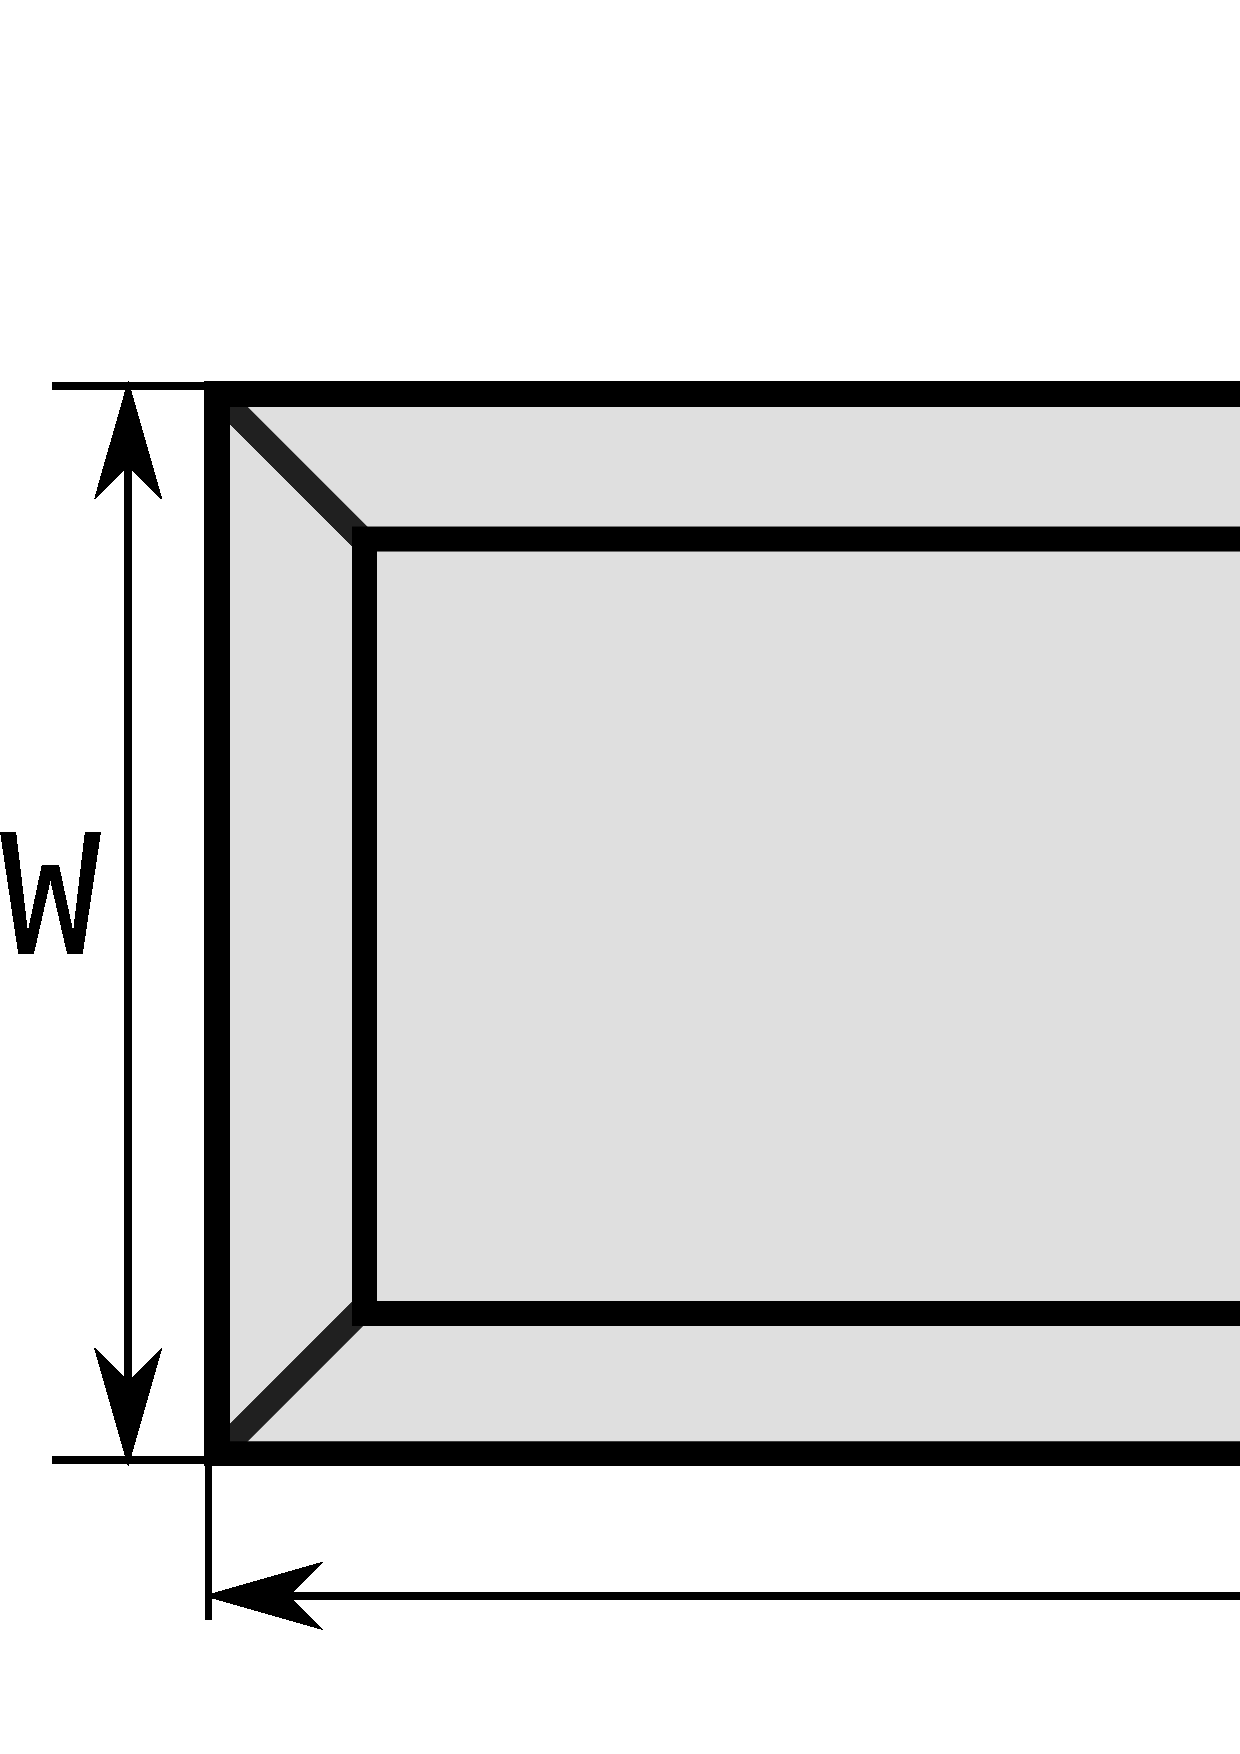
\includegraphics[width=.30\textwidth]{fig/cuts/AnisoPyramid2dxy.pdf}}
\hfill
\subfigure[Side view]{\raisebox{2mm}{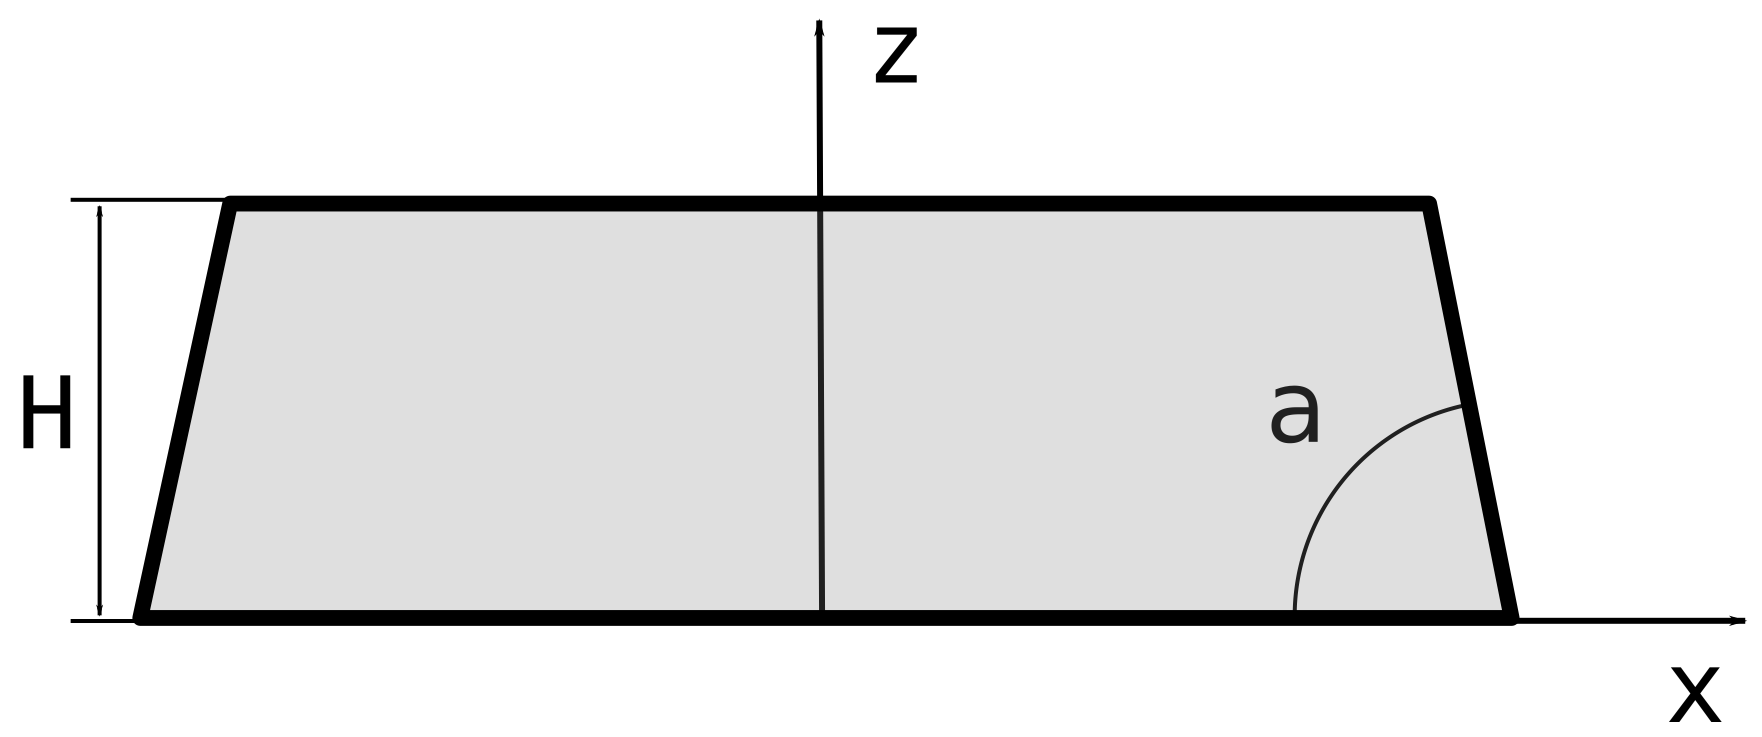
\includegraphics[width=.30\textwidth]{fig/cuts/AnisoPyramid2dxz.pdf}}}
\hfill
\caption{A truncated pyramid with a rectangular base.}
\end{figure}

\FloatBarrier

\paragraph{Syntax and parameters}\strut\\[-2ex plus .2ex minus .2ex]
\begin{lstlisting}
  FormFactorAnisoPyramid(double length, double width, double height, double alpha)
\end{lstlisting}
with the parameters
\begin{itemize}
\item \texttt{length} of the base, $L$,
\item \texttt{width} of the base, $W$,
\item \texttt{height}, $H$
\item \texttt{alpha}, angle between the base and a side face, $\alpha$.
\end{itemize}
They must fulfill
\begin{displaymath}
  H \le \frac{\tan\alpha}{2} \min\,(L,W).
\end{displaymath}

\paragraph{Form factor, volume, horizontal section}\strut\\
\begin{equation*}
  F \text{~: computed using the generic polyhedron form factor~\cite{ba:ffp},}
\end{equation*}
\begin{equation*}
  V= H \Big[LW - \dfrac{(L + W)H}{\tan\alpha} + \dfrac{4}{3} \dfrac{H^2}{\tan^2\alpha}\Big].
\end{equation*}
\begin{equation*}
  S=LW.
\end{equation*}

\paragraph{Examples}\strut\\
\begin{figure}[H]
\begin{center}
\includefinal{1\TW}{fig/ff2/ff_AnisoPyramid.pdf}
\end{center}
\caption{Normalized intensity $|F|^2/V^2$,
computed with $L=13$~nm, $W=8$~nm, $H=4.2$~nm, and $\alpha=60^\circ$,
for four different angles~$\omega$ of rotation around the $z$ axis.}
\label{fig:FFAnisoPyramidEx}
\end{figure}

\paragraph{History}\strut\\
Agrees with the \E{In-plane anisotropic pyramid} form factor of \IsGISAXS\
\cite[Eq.~2.40]{Laz08} \cite[Eq.~217]{ReLL09},
except for different parametrization.
This is \E{not} the \E{anisotropic pyramid} of \FitGISAXS,
which is a true pyramid with an off-center apex \cite{Bab13}.

Formfactors~$F(\q)$ have been checked against the different computation of \IsGISAXS,
and were found to fully agree.

%===============================================================================
\ffsection{Box (cuboid)} \label{SBox}
%===============================================================================
  \index{Box (form factor)}
  \index{Cuboid (form factor)}
  \index{Prism (form factor)!reactangular (Box)}
  \index{Platonic solids!cube}
  \index{FormFactorBox@\Code{FormFactorBox}}

\paragraph{Real-space geometry}\strut\\

\begin{figure}[H]
\hfill
\subfigure[Perspective]{\includefinal{.24\TW}{fig/blue/Box3d.png}}
\hfill
\subfigure[Top view]{\includefinal{.3\TW}{fig/cuts/Box2dxy.pdf}}
\hfill
\subfigure[Side view]{\raisebox{2mm}{\includefinal{.3\TW}{fig/cuts/Box2dxz.pdf}}}
\hfill
\caption{A rectangular cuboid.}
\end{figure}

\FloatBarrier

\paragraph{Syntax and parameters}\strut\\[-2ex plus .2ex minus .2ex]
\begin{lstlisting}
  FormFactorBox(double length, double width, double height)
\end{lstlisting}
with the parameters
\begin{itemize}
\item \texttt{length} of the base, $L$,
\item \texttt{width} of the base, $W$,
\item \texttt{height}, $H$.
\end{itemize}

\paragraph{Form factor, volume, horizontal section}

\begin{equation*}
F= L W H\exp\left(i q_z \frac{H}{2}\right) \sinc\left(q_x \frac{L}{2}\right)
\sinc\left(q_y \frac{W}{2}\right) \sinc\left(q_z \frac{H}{2}\right),
\end{equation*}
\begin{equation*}
  V= LWH,
\end{equation*}
\begin{equation*}
  S = LW.
\end{equation*}

\paragraph{Examples}\strut

\begin{figure}[H]
\begin{center}
\includefinal{1\TW}{fig/ff2/ff_Box.pdf}
\end{center}
\caption{Normalized intensity $|F|^2/V^2$,
computed with $L=18$~nm, $W=4.6$~nm, and $H=3$~nm,
for four different angles~$\omega$ of rotation around the $z$ axis.}
\end{figure}

\paragraph{History}\strut\\
Agrees with \E{Box} form factor of \IsGISAXS\
\cite[Eq.~2.38]{Laz08} \cite[Eq.~214]{ReLL09},
except for factors $1/2$ in the definitions of parameters $L$, $W$, $H$.


%===============================================================================
\ffsection{Cone (circular)} \label{SCone}
%===============================================================================
  \index{Cone (form factor)!circular}
  \index{Truncated cone (form factor)}
  \index{FormFactorCone@\Code{FormFactorCone}}

\paragraph{Real-space geometry}\strut\\

\begin{figure}[H]
\hfill
\subfigure[Perspective]{\includefinal{.24\TW}{fig/blue/Cone3d.png}}
\hfill
\subfigure[Top view]{\includefinal{.3\TW}{fig/cuts/Cone2dxy.pdf}}
\hfill
\subfigure[Side view]{\raisebox{3mm}{\includefinal{.3\TW}{fig/cuts/Cone2dxz.pdf}}}
\hfill
\caption{A truncated cone with circular base.}
\end{figure}

\paragraph{Syntax and parameters}\strut\\[-2ex plus .2ex minus .2ex]
\begin{lstlisting}
  FormFactorCone(double radius, double height, double alpha)
\end{lstlisting}
with the parameters
\begin{itemize}
\item \texttt{radius}, $R$,
\item \texttt{height}, $H$,
\item \texttt{alpha}, angle between the side and the base, $\alpha$.
\end{itemize}
They must fulfill
\begin{displaymath}
  H\le R\tan\alpha.
\end{displaymath}

\paragraph{Form factor, volume, horizontal section}\strut\\
Notation:
\begin{equation*}
  R_H \coloneqq R-\dfrac{H}{\tan \alpha}, \quad
  q_{\parallel} \coloneqq \sqrt{q_x^2+ q_y^2}, \quad
  \tilde{q}_z \coloneqq q_z \tan\alpha.
\end{equation*}
Results:
\begin{equation*}
  F = 2\pi \tan\alpha\; \e^{i\tilde{q}_z R}
      \int_{R_H}^R \!\d\rho\, \rho^2
        \frac{J_1(q_{\parallel}\rho)}{q_{\parallel}\rho}\,\e^{-i\tilde{q}_z \rho},
\end{equation*}
\begin{equation*}
  V = \dfrac{\pi}{3}\tan\alpha  \left( R^3 - R_H^3\right),
\end{equation*}
\begin{equation*}
  S=\pi R^2.
\end{equation*}

\paragraph{Examples}\strut

\begin{figure}[H]
\begin{center}
\includefinal{1\TW}{fig/ff2/ff_Cone.pdf}
\end{center}
\caption{Normalized intensity $|F|^2/V^2$,
computed with $R=4$~nm, $H=11$~nm, and $\alpha=75^\circ$,
for four different tilt angles~$\vartheta$ (rotation around the $y$ axis).}
\end{figure}

\paragraph{History}\strut\\
Agrees with \E{Cone} form factor of \IsGISAXS\
\cite[Eq.~2.28]{Laz08} \cite[Eq.~225]{ReLL09},
except for a substitution $z\to\rho$ in our expression for~$F$.


%===============================================================================
\ffsection{Cone6 (hexagonal)} \label{SCone6}
%===============================================================================
  \index{Cone (form factor)!hexagonal (Cone6)}
  \index{Pyramid (form factor)!hexagonal (Cone6)}
  \index{Truncated pyramid (form factor)!hexagonal (Cone6)}
  \index{FormFactorCone6@\Code{FormFactorCone6}}

\paragraph{Real-space geometry}\strut\\

\begin{figure}[H]
\hfill
\subfigure[Perspective]{\includefinal{.24\TW}{fig/blue/Cone63d.png}}
\hfill
\subfigure[Top view]{\includefinal{.3\TW}{fig/cuts/Cone62dxy.pdf}}
\hfill
\subfigure[Side view]{\raisebox{5mm}{\includefinal{.3\TW}{fig/cuts/Cone62dxz.pdf}}}
\hfill
\caption{A truncated pyramid, based on a regular hexagon}
\end{figure}

\FloatBarrier
\paragraph{Syntax and parameters}\strut\\[-2ex plus .2ex minus .2ex]
\begin{lstlisting}
  FormFactorCone6(double base_edge, double height, double alpha)
\end{lstlisting}
with the parameters
\begin{itemize}
\item \texttt{base\_edge}, edge of the regular hexagonal base, $R$,
\item \texttt{height}, $H$,
\item \texttt{alpha}, dihedral angle between the base and a side face, $\alpha$.
\end{itemize}
Note that the orthographic projection does not show~$\alpha$,
but the angle~$\beta$ between the base and a side edge.
They are related through $\sqrt{3}\tan \alpha = 2 \tan \beta$.
The following is written more conveniently in terms of~$\beta$.
The parameters must fulfill
\begin{displaymath}
  H \le (\tan\beta)R.
\end{displaymath}

\paragraph{Form factor, volume, horizontal section}\strut\\
\begin{equation*}
  F \text{~: computed using the generic polyhedron form factor~\cite{ba:ffp},}
\end{equation*}
\begin{equation*}
  V = \tan\beta  \left( R^3- \left(R-\frac{H}{\tan\beta}\right)^3 \right),
\end{equation*}
\begin{equation*}
  S =\dfrac{3\sqrt{3}R^2}{2}.
\end{equation*}

\paragraph{Examples}\strut

\begin{figure}[H]
\begin{center}
\includefinal{1\TW}{fig/ff2/ff_Cone6.pdf}
\end{center}
\caption{Normalized intensity $|F|^2/V^2$,
computed with $R=6$~nm, $H=5$~nm, and $\alpha=60^\circ$,
for four different angles~$\omega$ of rotation around the $z$ axis.}
\end{figure}

\paragraph{History}\strut\\
Our parametrization deviates from the form factor \E{Cone6} of \IsGISAXS
\cite[Eq.~2.32]{Laz08} \cite[Eq.~222]{ReLL09}.

Up to \BornAgain-1.5 computed by numeric integration, as in \IsGISAXS.
Since \BornAgain-1.6 higher speed and better accuracy are achieved
by using the generic polyhedron form factor \cite{ba:ffp},
with series expansions near singularities.

%===============================================================================
\ffsection{Cuboctahedron} \label{SCuboctahedron}
%===============================================================================
  \index{Cuboctahedron (form factor)}
  \index{Platonic solids!octahedron}
  \index{FormFactorCuboctahedron@\Code{FormFactorCuboctahedron}}

\paragraph{Real-space geometry}\strut\\

\begin{figure}[H]
\hfill
\subfigure[Perspective]{\includefinal{.24\TW}{fig/blue/Cuboctahedron3d.png}}
\hfill
\subfigure[Top view]{\includefinal{.3\TW}{fig/cuts/Cuboctahedron2dxy.pdf}}
\hfill
\subfigure[Side view]{\raisebox{2mm}{\includefinal{.3\TW}{fig/cuts/Cuboctahedron2dxz.pdf}}}
\hfill
\caption{A compound of two truncated pyramids with a common square base
and opposite orientations.}
\end{figure}

\FloatBarrier

\paragraph{Syntax and parameters}\strut\\[-2ex plus .2ex minus .2ex]
\begin{lstlisting}
  FormFactorCuboctahedron(double length, double height, double height_ratio, double alpha)
\end{lstlisting}
with the parameters
\begin{itemize}
\item \texttt{length} of the shared square base, $L$,
\item \texttt{height} of the bottom pyramid, $H$,
\item \texttt{height\_ratio} between the top and the bottom pyramid, $r_H$,
\item \texttt{alpha}, angle between the base and a side face, $\alpha$.
\end{itemize}
They must fulfill
\begin{displaymath}
  H \le \frac{\tan\alpha}{2} L
  \quad\text{and}\quad
  r_h H \le \frac{\tan\alpha}{2} L.
\end{displaymath}

\paragraph{Form factor, volume, horizontal section}\strut\\
\begin{equation*}
  F \text{~: computed using the generic polyhedron form factor~\cite{ba:ffp},}
\end{equation*}
\begin{equation*}
  V= \dfrac{1}{6} \tan(\alpha)L^3 \Big[ 2
         - \Big(1 - \dfrac{2H }{L\tan(\alpha)} \Big)^3
           - \Big(1 - \dfrac{2 r_H
             H}{L\tan(\alpha) }\Big)^3\Big],
\end{equation*}
\begin{equation*}
  S =L^2.
\end{equation*}

\paragraph{Examples}\strut

\begin{figure}[H]
\begin{center}
\includefinal{1\TW}{fig/ff2/ff_Cuboctahedron.pdf}
\end{center}
\caption{Normalized intensity $|F|^2/V^2$,
computed with $L=8$~nm, $H=5$~nm, $r_H=0.5$, and $\alpha=60^\circ$,
for four different angles~$\omega$ of rotation around the $z$ axis.}
\end{figure}

\paragraph{History}\strut\\
Agrees with \E{Cuboctahedron} form factor of \IsGISAXS\
\cite[Eq.~2.34]{Laz08} \cite[Eq.~218]{ReLL09},
except for different parametrization $L=2R_{\rm{\Code{IsGISAXS}}}$.
Since \BornAgain-1.6 implemented
using the generic polyhedron form factor \cite{ba:ffp}.


%===============================================================================
\ffsection{Cylinder} \label{SCylinder}
%===============================================================================
  \index{Cylinder (form factor)}
  \index{FormFactorCylinder@\Code{FormFactorCylinder}}

\paragraph{Real-space geometry}\strut\\

\begin{figure}[H]
\hfill
\subfigure[Perspective]{\includefinal{.24\TW}{fig/blue/Cylinder3d.png}}
\hfill
\subfigure[Top view]{\includefinal{.3\TW}{fig/cuts/Cylinder2dxy.pdf}}
\hfill
\subfigure[Side view]{\raisebox{-2.5mm}{\includefinal{.3\TW}{fig/cuts/Cylinder2dxz.pdf}}}
\hfill
\caption{An upright circular cylinder.}
\end{figure}

\paragraph{Syntax and parameters}\strut\\[-2ex plus .2ex minus .2ex]
\begin{lstlisting}
  FormFactorCylinder(double radius, double height)
\end{lstlisting}
with the parameters
\begin{itemize}
\item \texttt{radius} of the circular base, $R$,
\item \texttt{height}, $H$.
\end{itemize}

\paragraph{Form factor, volume, horizontal section}\strut\\
Notation:
\begin{equation*}
  q_{\parallel} \coloneqq \sqrt{q_x^2+q_y^2}.
\end{equation*}
Note that this does \E{not} involve the sesquilinear product
$|q_x|^2=q_x^* q_x$ but the plain product $q_xq_x$ of complex numbers
(and analogous for~$q_y$).

Results:
\begin{equation*}
  F=  2\pi R^2 H  \sinc\left(q_ z \frac{H}{2}\right) \exp\left(i q_ z \frac{H}{2}\right)
    \frac{J_1(q_{\parallel} R )}{q_{\parallel} R },
\end{equation*}
\begin{equation*}
  V = \pi R^2 H,
\end{equation*}
\begin{equation*}
  S=\pi R^2.
\end{equation*}

\paragraph{Examples}\strut

\begin{figure}[H]
\begin{center}
\includefinal{1\TW}{fig/ff2/ff_Cylinder.pdf}
\end{center}
\caption{Normalized intensity $|F|^2/V^2$,
computed with $R=3$~nm and $H=8.8$~nm,
for four different tilt angles~$\vartheta$ (rotation around the $y$ axis).}
\end{figure}

\paragraph{History and Derivation}\strut\\
For real wave vectors, this form factor is well known;
it goes back to Lord Rayleigh.
In \IsGISAXS, it has been implemented as form factor \E{Cylinder}
\cite[Eq.~2.27]{Laz08} \cite[Eq.~223]{ReLL09},
allowing for complex wavevectors.

Since it is not obvious that the standard formula also holds for complex~$\q$,
let us provide a derivation. We only consider the integral over the polar angle,
\begin{equation}
  I(\q) \coloneqq \int_0^{2\pi}\!\d\varphi\,\exp\left(iq_xr\sin\varphi+iq_yr\cos\varphi\right).
\end{equation}
With the abbreviations $a\coloneqq r(q_x+iq_y)/2$ and $b\coloneqq r(q_x-iq_y)/2$,
\begin{equation}
  I(\q) = \int_0^{2\pi}\!\d\varphi\,\exp\left(a\e^{i\varphi}-b\e^{-i\varphi}\right).
\end{equation}
Expansion of the exponential, combined with a binomial expansion of its argument, yields
\begin{equation}
  I(\q)
  = \int_0^{2\pi}\!\d\varphi\,
  \sum_{n=0}^\infty\sum_{k=0}^n(-)^k\frac{a^{n-k}b^{k}}{(n-k)!k!}\e^{i(n-2k)\varphi}.
\end{equation}
The integral over $\varphi$ vanishes except for $n=2k$. Hence
\begin{equation}
  I(\q)
  = 2\pi \sum_{k=0}^\infty(-)^k\frac{{\sqrt{ab}\,}^{2k}}{k!k!}
  = 2\pi J_0\left(rq_\parallel\right).
\end{equation}
Integration over~$r$ then yields the in-plane contribution to the form factor~$F(\q)$.


%===============================================================================
\ffsection{Dodecahedron} \label{SDodecahedron}
%===============================================================================
  \index{Dodecahedron (form factor)}
  \index{Platonic solids!dodecahedron}
  \index{FormFactorDodecahedron@\Code{FormFactorDodecahedron}}

\paragraph{Real-space geometry}\strut\\

\begin{figure}[H]
\strut\hfill
%\subfigure[Perspective]
{\includefinal{.24\TW}{fig/blue/Dodecahedron3d.png}}
%\hfill
%\subfigure[Top view]{\includefinal{.3\TW}{fig/cuts/Box2dxy.pdf}}
%\hfill
%\subfigure[Side view]{\raisebox{2mm}{\includefinal{.3\TW}{fig/cuts/Box2dxz.pdf}}}
\hfill\strut
\caption{A regular dodecahedron.}
\end{figure}

\FloatBarrier

\paragraph{Syntax and parameters}\strut\\[-2ex plus .2ex minus .2ex]
\begin{lstlisting}
  FormFactorDodecahedron(double edge)
\end{lstlisting}
with the parameter
\begin{itemize}
\item \texttt{edge}, length of one edge, $a$.
\end{itemize}

\paragraph{Form factor, volume, horizontal section}\strut\\
\begin{equation*}
  F \text{~: computed using the generic form factor of a polyhedron
             with inversion symmetry~\cite{ba:ffp},}
\end{equation*}
\begin{equation*}
  V= \frac{1}{4} (15+7\sqrt{5}) a^3 \approx 7.663\,a^3,
\end{equation*}
%\begin{equation*}
%  S = %% wait for Holden, Shapes, Space, and Symmetry
%\end{equation*}

\paragraph{Examples}\strut

\begin{figure}[H]
\begin{center}
\includefinal{1\TW}{fig/ff2/ff_Dodecahedron_sym.pdf}
\end{center}
\caption{Normalized intensity $|F|^2/V^2$,
computed with $a=3.2$~nm,
for three orientations of high symmetry:
$x$ axis perpendicular to a polygonal face;
vertex on the $x$ axis;
edge in the $xy$ plane and perpendicular to the $x$ axis.}
\end{figure}

\begin{figure}[H]
\begin{center}
\includefinal{1\TW}{fig/ff2/ff_Dodecahedron_asy.pdf}
\end{center}
\caption{Normalized intensity $|F|^2/V^2$,
computed with $a=3.2$~nm,
for three orientations of decreasing symmetry:
base pentagon in $xy$ plane and pointing in $x$ direction;
rotated by $13^\circ$ around the $z$ axis;
ditto, and tilted by $9^\circ$ around the $x$ axis.}
\end{figure}

\paragraph{History}\strut\\
New in \BornAgain-1.6,
based on the generic form factor of the polyhedron~\cite{ba:ffp}.


%===============================================================================
\ffsection{EllipsoidalCylinder} \label{SEllipsoidalCylinder}
%===============================================================================
  \index{Ellipsoidal cylinder (form factor)}
  \index{Cylinder (form factor)!ellipsoidal}
  \index{FormFactorEllipsoidalCylinder@\Code{FormFactorEllipsoidalCylinder}}

\paragraph{Real-space geometry}\strut\\

\begin{figure}[H]
\hfill
\subfigure[Perspective]{\includefinal{.24\TW}{fig/blue/EllipsoidalCylinder3d.png}}
\hfill
\subfigure[Top view]{\includefinal{.3\TW}{fig/cuts/EllipsoidalCylinder2dxy.pdf}}
\hfill
\subfigure[Side view]{\raisebox{4mm}{\includefinal{.3\TW}{fig/cuts/EllipsoidalCylinder2dxz.pdf}}}
\hfill
\caption{A upright cylinder whose cross section is an ellipse.}
\end{figure}

\paragraph{Syntax and parameters}\strut\\[-2ex plus .2ex minus .2ex]
\begin{lstlisting}
  FormFactorEllipsoidalCylinder(double radius_a, double radius_b, double height)
\end{lstlisting}
with the parameters
\begin{itemize}
\item \texttt{radius\_a}, in $x$ direction, $R_a$,
\item \texttt{radius\_b}, in $y$ direction, $R_b$,
\item \texttt{height}, $H$.
\end{itemize}

\paragraph{Form factor, volume, horizontal section}\strut\\
Notation:
\begin{equation*}
  \gamma \coloneqq \sqrt{(q_x R_a)^2+(q_y R_b)^2}
\end{equation*}
Results:
\begin{equation*}
F = 2\pi R_a R_b H \exp\left(i\frac{q_z H}{2}\right)
   \sinc\left(\frac{q_z H}{2}\right) \frac{J_1(\gamma)}{\gamma},
\end{equation*}
\begin{equation*}
  V = \pi R_a R_bH,
\end{equation*}
\begin{equation*}
  S = R_a R_b.
\end{equation*}

\paragraph{Examples}\strut

\begin{figure}[H]
\begin{center}
\includefinal{1\TW}{fig/ff2/ff_EllipsoidalCylinder.pdf}
\end{center}
\caption{Normalized intensity $|F|^2/V^2$,
computed with $R_a=6.3$~nm, $R_b=4.2$~nm and $H=3$~nm,
for four different angles~$\omega$ of rotation around the $z$ axis.}
\end{figure}

\paragraph{History}\strut\\
Agrees with the \IsGISAXS\ form factor
\E{Ellipsoid} \cite[Eq.~2.41, wrongly labeled in Fig.~2.4]{Laz08}
or \E{Ellipsoidal Cylinder} \cite[Eq.~224]{ReLL09}.


%===============================================================================
\ffsection{FullSphere} \label{SFullSphere}
%===============================================================================
  \index{Full sphere (form factor)}
  \index{Sphere (form factor)}
  \index{FormFactorFullSphere@\Code{FormFactorFullSphere}}

\paragraph{Real-space geometry}\strut\\

\begin{figure}[H]
\hfill
\subfigure[Perspective]{\includefinal{.24\TW}{fig/blue/FullSphere3d.png}}
\hfill
\subfigure[Top view]{\includefinal{.3\TW}{fig/cuts/FullSphere2dxy.pdf}}
\hfill
\subfigure[Side view]{\raisebox{-2mm}{\includefinal{.3\TW}{fig/cuts/FullSphere2dxz.pdf}}}
\hfill
\caption{A full sphere.}
\end{figure}

\FloatBarrier

\paragraph{Syntax and parameters}\strut\\[-2ex plus .2ex minus .2ex]
\begin{lstlisting}
  FormFactorFullSphere(double radius)
\end{lstlisting}
with the parameter
\begin{itemize}
\item \texttt{radius}, $R$.
\end{itemize}

\paragraph{Form factor, volume, horizontal section}\strut\\
Notation:
\begin{equation*}
  q \coloneqq \sqrt{q_x^2+q_y^2+q_z^2}.
\end{equation*}
Note that this does \E{not} involve the sesquilinear product
$|q_x|^2=q_x^* q_x$ but the plain product $q_xq_x$ of complex numbers
(and analogous for~$q_y$, $q_z$).
\begin{equation*}
F = \frac{4\pi}{q^3} \exp(iq_z R)\left[\sin(qR) - qR \cos(qR)\right],
\end{equation*}
\begin{equation*}
  V = \dfrac{4\pi}{3}R^3,
\end{equation*}
\begin{equation*}
  S= \pi R^2.
\end{equation*}

\paragraph{Example}\nopagebreak\strut\nopagebreak

\begin{figure}[H]
\begin{center}
\includefinal{.5\TW}{fig/ff2/ff_FullSphere.pdf}
\end{center}
\caption{Normalized intensity $|F|^2/V^2$,
computed with $R=3.9$~nm.}
\end{figure}

\paragraph{History and Derivation}\strut\\
For real wave vectors, this form factor is well known;
it goes back at least to Lord Rayleigh.
In \IsGISAXS, it has been implemented as form factor \E{Full sphere}
\cite[Eq.~2.36]{Laz08} \cite[Eq.~226]{ReLL09},
allowing for complex wavevectors.
Since it is not obvious that Rayleigh's formula also holds for complex~$\q$,
let us outline a derivation
(if you know a more elegant one, we would like to hear).

If the origin is at the center of the sphere, then the form factor is
\begin{equation}
I(\q,R)
 = \int_0^R\d r\, r^2\int_0^{\pi}\d\theta\,\sin\theta\int_0^{2\pi}\d\varphi
  \:\e^{i\q\r}
\end{equation}
with $\q\r
= q_x r\sin\theta\cos\varphi + q_y r\sin\theta\sin\varphi + q_z r\cos\theta$.
For the integration over $\varphi$,
see \cref{SCylinder} on the form factor of a cylinder:
\begin{equation}
  I(\q,R)
  = 2\pi \int_0^R \d r\,r^2 \int_0^{\pi} \d\theta\, \sin\theta
   \exp\left(i q_z \cos \theta\right) J_0\left(q_\parallel r\sin \theta\right)
\end{equation}
with $q_{\parallel}=\sqrt{q_x^2+q_y^2}$.
By symmetry, the imaginary part is zero,
so that the exponential reduces to a cosine:
\begin{equation}
  I(\q,R)
  = 2\pi \int_0^R \d r\,r^2 \int_0^{\pi} \d\theta\, \sin\theta
   \cos\left(q_z \cos \theta\right) J_0\left(q_\parallel r\sin \theta\right).
\end{equation}
Expand the cosine and the Bessel function:
\begin{equation}
  I(\q,R)
  = 2\pi \int_0^R \d r\,r^2 \int_0^{\pi} \d\theta\, \sin\theta
    \sum_{j=0}^\infty (-)^j \frac{(q_zr\cos\theta)^{2j}}{(2j)!}\,
    \sum_{k=0}^{\infty} (-)^k \frac{(q_\parallel r \sin\theta)^{2k}}{4^k k!^2}.
\end{equation}
Sort by powers of $r$, and integrate:
\begin{equation}
  I(\q,R)
  = 2\pi \sum_{n=0}^\infty (-)^n \frac{R^{2n+3}}{2n+3} \sum_{k=0}^n
    \frac{{q_z}^{2n-2k}}{(2n-2k)!}\,\frac{{q_\parallel}^{2k}}{4^k k!^2} \zeta(k,n)
\end{equation}
with
\begin{equation}
  \zeta(k,n)
  \coloneqq \int_0^{\pi} \d\theta\, \sin\theta
  (\cos\theta)^{2n-2k}(\sin\theta)^{2k}.
\end{equation}
This integral \cite[no.\ 2.512.4]{GrRy07} yields
\begin{equation}
  \zeta(k,n)
  = \frac{2^{2k+1}(2n-2k)! n! k!}{(2n+1)!(n-k)!}.
\end{equation}
Hence
\begin{equation}\label{ESphereU}
  I(\q,R)
  = 4\pi \sum_{n=0}^\infty (-)^n \frac{R^{2n+3}}{(2n+3)(2n+1)!}
    \sum_{k=0}^n \frac{n!}{(n-k)!k!}{q_z}^{2n-2k}{q_\parallel}^{2k}.
\end{equation}
The inner sum happens to be the binomial expansion of
$q^{2n}=\left({q_z}^2+{q_\parallel}^2\right)^n$.
Therefore \cref{ESphereU} coincides with the series expansion of
\begin{equation}
  I(\q,R)
  = 4\pi q^{-3} \left( \sin(qR) - qR\cos(qR) \right),
\end{equation}
which is what we wanted to prove.

%===============================================================================
\ffsection{FullSpheroid} \label{SFullSpheroid}
%===============================================================================
  \index{Full spheroid (form factor)}
  \index{Spheroid (form factor)}
  \index{FormFactorFullSpheroid@\Code{FormFactorFullSpheroid}}

\paragraph{Real-space geometry}\strut\\

\begin{figure}[H]
\hfill
\subfigure[Perspective]{\includefinal{.24\TW}{fig/blue/FullSpheroid3d.png}}
\hfill
\subfigure[Top view]{\includefinal{.3\TW}{fig/cuts/FullSpheroid2dxy.pdf}}
\hfill
\subfigure[Side view]{\raisebox{-3mm}{\includefinal{.3\TW}{fig/cuts/FullSpheroid2dxz.pdf}}}
\hfill
\caption{A full spheroid, generated by rotating an ellipse around the vertical axis.}
\end{figure}

\FloatBarrier

\paragraph{Syntax and parameters}\strut\\[-2ex plus .2ex minus .2ex]
\begin{lstlisting}
  FormFactorFullSpheroid(double radius, double height)
\end{lstlisting}
with the parameters
\begin{itemize}
\item \texttt{radius}, $R$,
\item \texttt{height}, $H$.
\end{itemize}

\paragraph{Form factor, volume, horizontal section}\strut\\
Notation:
\begin{equation*}
 R_z \coloneqq R\sqrt{1-\frac{4z^2}{H^2}},\quad
 q_\plll \coloneqq \sqrt{q_x^2+q_y^2}.
\end{equation*}
Results:
\begin{equation*}
  F = 4\pi \exp(i q_z H/2) \int_0^{H/2} \!\d z\,
     R_z^2 \frac{J_1(q_{\parallel}R_z)}{q_{\parallel}R_z} \cos(q_z z),
\end{equation*}
\begin{equation*}
  V =\dfrac{2}{3}R^2H,
\end{equation*}
\begin{equation*}
  S =\pi R^2.
\end{equation*}

\paragraph{Example}\strut

\begin{figure}[H]
\begin{center}
\includefinal{.5\TW}{fig/ff2/ff_FullSpheroid.pdf}
\end{center}
\caption{Normalized intensity $|F|^2/V^2$,
computed with $R=3.5$~nm and $H=9.8$~nm.}
% changes very little under tilt !
\end{figure}

\paragraph{History}\strut\\
Agrees with the \E{Full spheroid} form factor of \IsGISAXS\
\cite[Eq.~2.37]{Laz08} \cite[Eq.~227]{ReLL09},
with corrected volume formula.
We also discovered a wrong factor of~2 in the \IsGISAXS\ code.


%===============================================================================
\ffsection{HemiEllipsoid} \label{SHemiEllipsoid}
%===============================================================================
  \index{Hemi ellipsoid (form factor)}
  \index{Ellipsoid (form factor)!truncated}
  \index{Truncated ellipsoid (form factor)}
  \index{FormFactorHemiEllipsoid@\Code{FormFactorHemiEllipsoid}}

\paragraph{Real-space geometry}\strut\\

\begin{figure}[H]
\hfill
\subfigure[Perspective]{\includefinal{.24\TW}{fig/blue/HemiEllipsoid3d.png}}
\hfill
\subfigure[Top view]{\includefinal{.3\TW}{fig/cuts/HemiEllipsoid2dxy.pdf}}
\hfill
\subfigure[Side view]{\raisebox{5mm}{\includefinal{.3\TW}{fig/cuts/HemiEllipsoid2dxz.pdf}}}
\hfill
\caption{An horizontally oriented ellipsoid, truncated at the central plane.}
\end{figure}

\paragraph{Syntax and parameters}\strut\\[-2ex plus .2ex minus .2ex]
\begin{lstlisting}
  FormFactorHemiEllipsoid(double radius_a, double radius_b, double height)
\end{lstlisting}
with the parameters
\begin{itemize}
\item \texttt{radius\_a}, in $x$ direction, $R_a$,
\item \texttt{radius\_b}, in $y$ direction, $R_b$,
\item \texttt{height}, equal to radius in $z$ direction, $H$
\end{itemize}

\paragraph{Form factor, volume, horizontal section}\strut\\
Notation:
\begin{equation*}
 r_{a,z} \coloneqq R_a \sqrt{1-\left(\dfrac{z}{H} \right)^2},\quad
 r_{b,z} \coloneqq R_b \sqrt{1-\left(\dfrac{z}{H} \right)^2}, \quad
 \gamma_z =\sqrt{(q_x r_{a,z})^2+(q_y r_{b,z})^2}.
\end{equation*}
Results:
\begin{equation*}
  F = 2\pi \int_0^{H} \!\d z\, r_{a,z} r_{b,z}
                               \frac{J_1(\gamma_z)}{\gamma_z}\exp(iq_z z),
\end{equation*}
\begin{equation*}
  V = \dfrac{2}{3}\pi R_a R_bH,
\end{equation*}
\begin{equation*}
  S =\pi R_a R_b.
\end{equation*}

\paragraph{Examples}\strut

\begin{figure}[H]
\begin{center}
\includefinal{1\TW}{fig/ff2/ff_HemiEllipsoid.pdf}
\end{center}
\caption{Normalized intensity $|F|^2/V^2$,
computed with $R_a=10$~nm, $R_b=3.8$~nm and $H=3.2$~nm,
for four different angles~$\omega$ of rotation around the $z$ axis.}
\end{figure}

\paragraph{History}\strut\\
Agrees with the \IsGISAXS\ form factor
\E{Anisotropic hemi-ellipsoid}
\cite[Eq.~2.42, with wrong sign in the $z$-dependent phase factor]{Laz08}
or \E{Hemi-spheroid} \cite[Eq.~229]{ReLL09}.


%===============================================================================
\ffsection{Icosahedron} \label{SIcosahedron}
%===============================================================================
  \index{Icosahedron (form factor)}
  \index{Platonic solids!icosahedron}
  \index{FormFactorIcosahedron@\Code{FormFactorIcosahedron}}

\paragraph{Real-space geometry}\strut\\

\begin{figure}[H]
\strut\hfill
%\subfigure[Perspective]
{\includefinal{.24\TW}{fig/blue/Icosahedron3d.png}}
%\hfill
%\subfigure[Top view]{\includefinal{.3\TW}{fig/cuts/Box2dxy.pdf}}
%\hfill
%\subfigure[Side view]{\raisebox{2mm}{\includefinal{.3\TW}{fig/cuts/Box2dxz.pdf}}}
\hfill\strut
\caption{A regular icosahedron.}
\end{figure}

\FloatBarrier

\paragraph{Syntax and parameters}\strut\\[-2ex plus .2ex minus .2ex]
\begin{lstlisting}
  FormFactorIcosahedron(double edge)
\end{lstlisting}
with the parameter
\begin{itemize}
\item \texttt{edge}, length of one edge, $a$.
\end{itemize}

\paragraph{Form factor, volume, horizontal section}\strut\\
\begin{equation*}
  F \text{~: computed using the generic form factor of a polyhedron
             with inversion symmetry~\cite{ba:ffp},}
\end{equation*}
\begin{equation*}
  V= \frac{5}{12} (3+\sqrt5)a^3 \approx 2.182\,a^3
\end{equation*}
%\begin{equation*}
%  S = %% wait for Holden, Shapes, Space, and Symmetry
%\end{equation*}

\paragraph{Examples}\strut

\begin{figure}[H]
\begin{center}
\includefinal{1\TW}{fig/ff2/ff_Icosahedron_sym.pdf}
\end{center}
\caption{Normalized intensity $|F|^2/V^2$,
computed with $a=4.8$~nm,
for three orientations of high symmetry:
$x$ axis perpendicular to a polygonal face;
vertex on the $x$ axis;
edge in the $xy$ plane and perpendicular to the $x$ axis.}
\end{figure}

\begin{figure}[H]
\begin{center}
\includefinal{1\TW}{fig/ff2/ff_Icosahedron_asy.pdf}
\end{center}
\caption{Normalized intensity $|F|^2/V^2$,
computed with $a=4.8$~nm,
for three orientations of decreasing symmetry:
base pentagon in $xy$ plane and pointing in $x$ direction;
rotated by $13^\circ$ around the $z$ axis;
ditto, and tilted by $9^\circ$ around the $x$ axis.}
\end{figure}

\paragraph{History}\strut\\
New in \BornAgain-1.6,
based on the generic form factor of the polyhedron~\cite{ba:ffp}.


%===============================================================================
\ffsection{Prism3 (triangular)} \label{SPrism3}
%===============================================================================
  \index{Prism (form factor)!triangular (Prism3)}
  \index{FormFactorPrism3@\Code{FormFactorPrism3}}

\paragraph{Real-space geometry}\strut\\

\begin{figure}[H]
\hfill
\subfigure[Perspective]{\includefinal{.24\TW}{fig/blue/Prism33d.png}}
\hfill
\subfigure[Top view]{\includefinal{.3\TW}{fig/cuts/Prism32dxy.ps}}
\hfill
\subfigure[Side view]{\includefinal{.3\TW}{fig/cuts/Prism32dxz.ps}}
\hfill
\caption{A prism based on an equilateral triangle.}
\end{figure}

\FloatBarrier

\paragraph{Syntax and parameters}\strut\\[-2ex plus .2ex minus .2ex]
\begin{lstlisting}
  FormFactorPrism3(double length, double height)
\end{lstlisting}
with the parameters
\begin{itemize}
\item \texttt{length} of one base edge, $L$,
\item \texttt{height}, $H$.
\end{itemize}

\paragraph{Form factor, volume, horizontal section}\strut\\
\begin{equation*}
F = H \sinc\left(q_z\frac{H}{2}\right) \exp\left(-i q_z\frac{ H}{2}\right) F_\parallel(\q_\parallel)
\end{equation*}
with the form factor $F_\parallel$ of the base triangle
computed using the generic form factor of a planar polygon \cite{ba:ffp},
\begin{equation*}
  V= \dfrac{\sqrt{3}}{4} H L^2,
\end{equation*}
\begin{equation*}
  S =\dfrac{\sqrt{3}}{4}L^2.
\end{equation*}

\paragraph{Examples}\strut

\begin{figure}[H]
\begin{center}
\includefinal{1\TW}{fig/ff2/ff_Prism3.pdf}
\end{center}
\caption{Normalized intensity $|F|^2/V^2$,
computed with $L=13.8$~nm and $H=3$~nm,
for four different angles~$\omega$ of rotation around the $z$ axis.}
\label{fig:FFprism3Ex}
\end{figure}

\paragraph{History}\strut\\
Has been validated against the \E{Prism3} form factor of \IsGISAXS\
\cite[Eq.~2.29]{Laz08} \cite[Eq.~219]{ReLL09}.
Note the different parameterization $L= 2 R_{\rm{\Code{IsGISAXS}}}$.
In \FitGISAXS\ just called \E{Prism} \cite{Bab13}.
In \BornAgain-1.6,
redefined to let the $x$ axis point along a symmetry axis
(rotated by $30^\circ$ with respect to the previous version).

Reimplemented in \BornAgain-1.6 using the generic form factor
of a polygonal prism \cite{ba:ffp},
to achieve numerical stability near the removable singularity at $q\to0$.

%===============================================================================
\ffsection{Prism6 (hexagonal)} \label{SPrism6}
%===============================================================================
  \index{Prism (form factor)!hexagonal (Prism6)}
  \index{FormFactorPrism6@\Code{FormFactorPrism6}}

\paragraph{Real-space geometry}\strut\\

\begin{figure}[H]
\hfill
\subfigure[Perspective]{\includefinal{.24\TW}{fig/blue/Prism63d.png}}
\hfill
\subfigure[Top view]{\includefinal{.3\TW}{fig/cuts/Prism62dxy.pdf}}
\hfill
\subfigure[Side view]{\raisebox{-3mm}{\includefinal{.3\TW}{fig/cuts/Prism62dxz.pdf}}}
\hfill
\caption{A prism based on a regular hexagon.}
\end{figure}

\FloatBarrier

\paragraph{Syntax and parameters}\strut\\[-2ex plus .2ex minus .2ex]
\begin{lstlisting}
  FormFactorPrism6(double radius, double height)
\end{lstlisting}
with the parameters
\begin{itemize}
\item \texttt{radius} of the hexagonal base, $R$,
\item \texttt{height}, $H$.
\end{itemize}

\paragraph{Form factor, volume, horizontal section}\strut\\
\begin{equation*}
F = H \sinc\left(q_z\frac{H}{2}\right) \exp\left(-i q_z\frac{ H}{2}\right) F_\parallel(\q_\parallel)
\end{equation*}
with the form factor $F_\parallel$ of the base hexagon
computed using the generic form factor of a planar polygon
with two-fold symmetry~($S_2$) \cite{ba:ffp},
\begin{equation*}
  V = \dfrac{3\sqrt{3}}{2}H R^2,
\end{equation*}
\begin{equation*}
  S =\dfrac{3\sqrt{3}R^2}{2}.
\end{equation*}

\paragraph{Examples}\strut\nopagebreak

\begin{figure}[H]
\begin{center}
\includefinal{1\TW}{fig/ff2/ff_Prism6.pdf}
\end{center}
\caption{Normalized intensity $|F|^2/V^2$,
computed with $R=5.7$~nm and $H=3$~nm,
for four different angles~$\omega$ of rotation around the $z$ axis.}
\label{fig:FFprism6Ex}
\end{figure}

\paragraph{History}\strut\\
Has been validated against the \E{Prism6} form factor of \IsGISAXS\
\cite[Eq.~2.31]{Laz08} \cite[Eq.~221]{ReLL09},
which has different parametrization
and lacks a factor $H$ in $F(\q)$.

Reimplemented in \BornAgain-1.5 using the generic form factor
of a polygonal prism with symmetry~$S_2$ \cite{ba:ffp},
to achieve numerical stability near the removable singularity at $q\to0$.


%===============================================================================
\ffsection{Pyramid (square-based)}\label{SPyramid}
%===============================================================================
  \index{Pyramid (form factor)!square}
  \index{Truncated pyramid (form factor)!square}
  \index{FormFactorPyramid@\Code{FormFactorPyramid}}

\paragraph{Real-space geometry}\strut\\

\begin{figure}[H]
\hfill
\subfigure[Perspective]{\includefinal{.24\TW}{fig/blue/Pyramid3d.png}}
\hfill
\subfigure[Top view]{\includefinal{.3\TW}{fig/cuts/Pyramid2dxy.pdf}}
\hfill
\subfigure[Side view]{\raisebox{2mm}{\includefinal{.3\TW}{fig/cuts/Pyramid2dxz.pdf}}}
\hfill
\caption{A truncated pyramid with a square base.}
\end{figure}

\FloatBarrier

\paragraph{Syntax and parameters}\strut\\[-2ex plus .2ex minus .2ex]
\begin{lstlisting}
  FormFactorPyramid(double length, double height, double alpha)
\end{lstlisting}
with the parameters
\begin{itemize}
\item \texttt{length} of one edge of the square base, $L$,
\item \texttt{height}, $H$,
\item \texttt{alpha}, angle between the base and a side face, $\alpha$,
\end{itemize}
They must fulfill
\begin{displaymath}
  H \le \frac{\tan\alpha}{2}L.
\end{displaymath}

\paragraph{Form factor, volume, horizontal section}\strut\\
\begin{equation*}
  F \text{~: computed using the generic polyhedron form factor~\cite{ba:ffp},}
\end{equation*}
\begin{equation*}
  V = \dfrac{1}{6}  L^3 \tan\alpha\left[ 1
             - \left(1 - \dfrac{2H}{L\tan\alpha}\right)^3 \right],,
\end{equation*}
\begin{equation*}
  S = L^2.
\end{equation*}

\paragraph{Examples}\strut

\begin{figure}[H]
\begin{center}
\includefinal{1\TW}{fig/ff2/ff_Pyramid.pdf}
\end{center}
\caption{Normalized intensity $|F|^2/V^2$,
computed with $L=10$~nm, $H=4.2$~nm and $\alpha=60^{\circ}$,
for four different angles~$\omega$ of rotation around the $z$ axis.}
\end{figure}

\paragraph{History}\strut\\
Corresponds to \E{Pyramid} form factor of \IsGISAXS\
\cite[Eq.~2.31]{Laz08} \cite[Eq.~221]{ReLL09},
except for different parametrization $L=2R_{\rm{\Code{IsGISXAXS}}}$
and a corrected sign.

Reimplemented in \BornAgain-1.6 using the generic form factor
of a polygonal prism \cite{ba:ffp},
to achieve numerical stability near the removable singularity at $q\to0$.


%===============================================================================
\ffsection{Tetrahedron} \label{STetrahedron}
%===============================================================================
  \index{Tetrahedron (form factor)}
  \index{Truncated tetrahedron (form factor)}
  \index{Platonic solids!tetrahedron}
  \index{FormFactorTetrahedron@\Code{FormFactorTetrahedron}}

\paragraph{Real-space geometry}\strut\\

\noindent
Incorrectly named so, since it actually has five, not four surfaces.

\begin{figure}[H]
\hfill
\subfigure[Perspective]{\includefinal{.24\TW}{fig/blue/Tetrahedron3d.png}}
\hfill
\subfigure[Top view]{\includefinal{.3\TW}{fig/cuts/Tetrahedron2dxy.ps}}
\hfill
\subfigure[Side view]{\includefinal{.3\TW}{fig/cuts/Tetrahedron2dxz.ps}}
\hfill
\caption{A truncated pyramid, based on an equilateral triangle.}
\end{figure}

\FloatBarrier

\paragraph{Syntax and parameters}\strut\\[-2ex plus .2ex minus .2ex]
\begin{lstlisting}
  FormFactorTetrahedron(double length, double height, double alpha)
\end{lstlisting}
with the parameters
\begin{itemize}
\item \texttt{length} of one edge of the equilateral triangular base, $L$,
\item \texttt{height}, $H$,
\item \texttt{alpha}, dihedral angle between the base and a side face, $\alpha$.
\end{itemize}
They must fulfill
\begin{displaymath}
  H\le \frac{\tan{\alpha}}{2\sqrt{3}} L.
\end{displaymath}
The orthographic projection also shows the angle~$\beta$ between the base and a side edge.
It is related to the dihedral angle through $\tan \alpha = 2 \tan \beta$.

\paragraph{Form factor, volume, horizontal section}\strut\\
\begin{equation*}
  F\text{~: computed using the generic polyhedron form factor~\cite{ba:ffp},}
\end{equation*}
\begin{equation*}
  V= \dfrac{\tan(\alpha) L^3}{24} \left[1- \left(1 -
  \dfrac{2\sqrt{3} H}{L \tan(\alpha)} \right)^3\right],
\end{equation*}
\begin{equation*}
  S =\dfrac{\sqrt{3}}{4}L^2.
\end{equation*}

\paragraph{Examples}\strut

\begin{figure}[H]
\begin{center}
\includefinal{1\TW}{fig/ff2/ff_Tetrahedron.pdf}
\end{center}
\caption{Normalized intensity $|F|^2/V^2$,
computed with $L=12$~nm, $H=8$~nm, and $\alpha=75^\circ$,
for four different angles~$\omega$ of rotation around the $z$ axis.
The low symmetry requires other angular ranges than used in most other figures.}
\end{figure}

\paragraph{History}\strut\\
Previous implementations as \E{Tetrahedron} in \IsGISAXS\
\cite[Eq.~2.30]{Laz08} \cite[Eq.~220]{ReLL09},
and as  \E{Truncated tetrahedron} in \FitGISAXS\ \cite{Bab13}.
In \BornAgain-1.6,
redefined to let the $x$ axis lie in a mirror plane
(rotated by $30^\circ$ with respect to the previous version).

Up to \BornAgain-1.5, we computed the form factor by numeric integration, as in \IsGISAXS.
Since \BornAgain-1.6 higher speed and accuracy are achieved
by using the generic polyhedron form factor \cite{ba:ffp},
with series expansions near singularities.

%===============================================================================
\ffsection{TruncatedCube} \label{STruncatedCube}
%===============================================================================
  \index{Cube (form factor)!facetted}
  \index{Facetted cube (form factor)}
  \index{FormFactorTruncatedCube@\Code{FormFactorTruncatedCube}}

\paragraph{Real-space geometry}\strut\\

\begin{figure}[H]
\hfill
\subfigure[Perspective]{\includefinal{.24\TW}{fig/blue/TruncatedCube3d.png}}
\hfill
\subfigure[Top view]{\includefinal{.3\TW}{fig/cuts/Truncatedcube2dxy.pdf}}
\hfill
\subfigure[Side view]{\includefinal{.3\TW}{fig/cuts/Truncatedcube2dxz.pdf}}
\hfill
\caption{A cube whose eight vertices have been removed.
The truncated part of each vertex is a trirectangular tetrahedron.}
\end{figure}

\FloatBarrier

\paragraph{Syntax and parameters}\strut\\[-2ex plus .2ex minus .2ex]
\begin{lstlisting}
  FormFactorTruncatedCube(double length, double removed_length)
\end{lstlisting}
with the parameters
\begin{itemize}
\item \texttt{length} of the full cube, $L$,
\item \texttt{removed\_length}, side length of the trirectangular tetrahedron removed from the cube's vertices, $t$.
\end{itemize}
They must fulfill
\begin{displaymath}
  t \le L/2.
\end{displaymath}

\paragraph{Form factor, volume, horizontal section}\strut\\
\begin{equation*}
  F \text{~: computed using the generic form factor of a polyhedron
             with inversion symmetry~\cite{ba:ffp},}
\end{equation*}
\begin{equation*}
  V = L^3 - \dfrac{4}{3}t^3,
\end{equation*}
\begin{equation*}
  S = L^2.
\end{equation*}

\paragraph{Examples}\strut

\begin{figure}[H]
\begin{center}
\includefinal{1\TW}{fig/ff2/ff_TruncatedCube.pdf}
\end{center}
\caption{Normalized intensity $|F|^2/V^2$,
computed with $L=25$~nm, $W=10$~nm, $H=8$~nm, and $d=5$~nm,
for four different angles~$\omega$ of rotation around the $z$ axis.}
\end{figure}

\paragraph{History}\strut\\
Motivated by \cite{HeSS74}.
Reimplemented in \BornAgain-1.6 using the generic form factor
of a polygonal prism \cite{ba:ffp}.


%===============================================================================
\ffsection{TruncatedSphere}\label{STruncatedSphere}
%===============================================================================
  \index{Sphere (form factor)!truncated}
  \index{Truncated sphere (form factor)}
  \index{FormFactorTruncatedSphere@\Code{FormFactorTruncatedSphere}}

\paragraph{Real-space geometry}\strut\\

\begin{figure}[H]
\hfill
\subfigure[Perspective]{\includefinal{.24\TW}{fig/blue/Sphere3d.png}}
\hfill
\subfigure[Top view]{\includefinal{.3\TW}{fig/cuts/Sphere2dxy.pdf}}
\hfill
\subfigure[Side view]{\raisebox{-2mm}{\includefinal{.3\TW}{fig/cuts/Sphere2dxz.pdf}}}
\hfill
\caption{A truncated sphere.}
\end{figure}
\FloatBarrier

\paragraph{Syntax and parameters}\strut\\[-2ex plus .2ex minus .2ex]
\begin{lstlisting}
  FormFactorTruncatedSphere(double radius, double height)
\end{lstlisting}
with the parameters
\begin{itemize}
\item \texttt{radius}, $R$,
\item \texttt{height}, $H$.
\end{itemize}
They must fulfill
\begin{displaymath}
   0 < H\leq 2R.
\end{displaymath}

\paragraph{Form factor, volume, horizontal section}\strut\\
Notation:
\begin{equation*}
  q_{\parallel} \coloneqq \sqrt{q_x^2+q_y^2},\quad
  R_z \coloneqq \sqrt{R^2-z^2}.
\end{equation*}
Results:
\begin{equation*}
F= 2\pi \exp[i q_z (H-R)]\int_{R-H}^{R}\!\d z\, R_z^2
       \frac{J_1(q_{\parallel} R_z) }{q_{\parallel} R_z} \exp(i q_z z) dz,
\end{equation*}
\begin{equation*}
  V=\pi R^3 \left[\dfrac{2}{3} + \dfrac{H-R}{R} - \dfrac{1}{3}\left(\dfrac{H-R}{R}\right)^3\right],
\end{equation*}
\begin{equation*}
  S = \left\{\begin{array}{ll} \pi R^2, & H \geq R \\
         \pi\left(2RH-H^2\right), & H < R \end{array}\right..
\end{equation*}

\paragraph{Example}\strut

\begin{figure}[H]
\begin{center}
\includefinal{1\TW}{fig/ff2/ff_TruncatedSphere.pdf}
\end{center}
\caption{Normalized intensity $|F|^2/V^2$,
computed with $R=4.2$~nm and $H=6.1$~nm,
for four different tilt angles~$\vartheta$ (rotation around the $y$ axis).}
\end{figure}

\paragraph{History}\strut\\
Agrees with the \IsGISAXS\ form factor
\E{Sphere} \cite[Eq.~2.33]{Laz08} or
\E{Truncated sphere} \cite[Eq.~228]{ReLL09}.


%===============================================================================
\ffsection{TruncatedSpheroid} \label{STruncatedSpheroid}
%===============================================================================
  \index{Spheroid (form factor)!truncated}
  \index{Truncated spheroid (form factor)}
  \index{FormFactorTruncatedSpheroid@\Code{FormFactorTruncatedSpheroid}}

\paragraph{Real-space geometry}\strut\\

\begin{figure}[H]
\hfill
\subfigure[Perspective]{\includefinal{.24\TW}{fig/blue/Spheroid3d.png}}
\hfill
\subfigure[Top view]{\raisebox{5mm}{\includefinal{.3\TW}{fig/cuts/Spheroid2dxy.pdf}}}
\hfill
\subfigure[Side view]{\includefinal{.3\TW}{fig/cuts/Spheroid2dxz.pdf}}
\hfill
\caption{A vertically oriented, horizontally truncated spheroid.}
\end{figure}

\paragraph{Syntax and parameters}\strut\\[-2ex plus .2ex minus .2ex]
\begin{lstlisting}
  FormFactorTruncatedSpheroid(double radius, double height, double height_flattening)
\end{lstlisting}
with the parameters
\begin{itemize}
\item \texttt{radius}, $R$,
\item \texttt{height}, $H$.
\item \texttt{height\_flattening}, $f_p$.
\end{itemize}
They must fulfill
\begin{displaymath}
  0< \dfrac{H}{R}\le 2f_p.
\end{displaymath}

\paragraph{Form factor, volume, horizontal section}\strut\\
Notation:
\begin{equation*}
  q_{\parallel} \coloneqq \sqrt{q_x^2+q_y^2}, \quad
  R_z \coloneqq \sqrt{R^2-z^2/f_p^2}.
\end{equation*}
Results:
\begin{equation*}
F =   2\pi \exp[iq_z(H-f_pR)] \int_{f_p R-H}^{f_p R} \!\d z\,
     R_z^2\frac{J_1(q_{\parallel}R_z)}{q_{\parallel}R_z} \exp(i q_z z)
\end{equation*}
\begin{equation*}
  V = \dfrac{\pi R H^2}{f_p}  \Big(1-\dfrac{H}{3f_p R}\Big),
\end{equation*}
\begin{equation*}
  S = \left\{\begin{array}{ll} \pi R^2, & H \geq f_pR \\
         \pi\left(\dfrac{2RH}{f_p}-\dfrac{H^2}{f_p^2}\right), & H < R \end{array}\right..
\end{equation*}

\paragraph{Example}\strut

\begin{figure}[H]
\begin{center}
\includefinal{1\TW}{fig/ff2/ff_TruncatedSpheroid.pdf}
\end{center}
\caption{Normalized intensity $|F|^2/V^2$,
computed with $R=3.3$~nm, $H=9.8$~nm, and $f_p=1.8$,
for four different tilt angles~$\vartheta$ (rotation around the $y$ axis).}
\end{figure}

\paragraph{History}\strut\\
Agrees with the \IsGISAXS\ form factor
\E{Sphere} \cite[Eq.~2.33]{Laz08} or
\E{TruncatedSpheroid} \cite[Eq.~228]{ReLL09}.
% Note an erroneous factor~2 in the expression of the volume
% in the \Code{IsGISAXS} manual.

\index{Shape transform!catalogue|)}
\index{Form factor!catalogue|)}

%%%%%%%%%%%%%%%%%%%%%%%%%%%%%%%%%%%%%%%%%%%%%%%%%%%%%%%%%%%%%%%%%%%%%%%%%%%%%%%%
\section{Ripples}\label{SRipple}
%%%%%%%%%%%%%%%%%%%%%%%%%%%%%%%%%%%%%%%%%%%%%%%%%%%%%%%%%%%%%%%%%%%%%%%%%%%%%%%%


%===============================================================================
\ffsection{Ripple1 (sinusoidal)} \label{SRipple1}
%===============================================================================
  \index{Ripple (form factor)!sinusoidal (Ripple1)}
  \index{Sinusoidal ripple (form factor)}
  \index{FormFactorRipple1@\Code{FormFactorRipple1}}

\paragraph{Real-space geometry}\strut\\

\begin{figure}[H]
\hfill
\subfigure[Perspective]{\includefinal{.24\TW}{fig/blue/Ripple13d.png}}
\hfill
\subfigure[Top view]{\includefinal{.3\TW}{fig/cuts/Ripple12dxy.pdf}}
\hfill
\subfigure[Side view]{\includefinal{.3\TW}{fig/cuts/Ripple12dyz.pdf}}
\hfill
\caption{A ripple with a sinusoidal profile.}
\end{figure}

\paragraph{Syntax and parameters}\strut\\[-2ex plus .2ex minus .2ex]
\begin{lstlisting}
  FormFactorRipple1(double length, double width, double height)
\end{lstlisting}
with the parameters
\begin{itemize}
\item \texttt{length}, $L$,
\item \texttt{width}, $W$,
\item \texttt{height}, $H$.
\end{itemize}

The ripple is modelled as a surface
\begin{equation*}
  Z(y) = \frac{H}{2}\left[ 1 + \cos\frac{2\pi y}{W} \right].
\end{equation*}

\paragraph{Form factor}\strut\\
Using the inverse profile
\begin{equation*}
  Y(z) = \frac{W}{2\pi}\text{arccos}\left( \frac{2z}{H}-1 \right),
\end{equation*}
the form factor is computed by numeric integration:
\begin{equation*}
F = L \sinc\left(\frac{q_xL}{2}\right)
   \int_0^H\!\d z\,\e^{iq_zz}\, 2Y(z)\sinc\left(q_y Y(z)\right).
\end{equation*}
The integration is substantially accelerated by the substitution
$u=\text{arccos}( 2z/H-1)$.

\paragraph{Volume, horizontal section}\strut\\
\begin{equation*}
  V = \dfrac{L W H}{2},
\end{equation*}
\begin{equation*}
  S = L W.
\end{equation*}

\paragraph{Examples}\strut

\begin{figure}[H]
\begin{center}
\includefinal{1\TW}{fig/ff2/ff_Ripple1.pdf}
\end{center}
\caption{Normalized intensity $|F|^2/V^2$,
computed with $L=25$~nm, $W=10$~nm and $H=8$~nm,
for four different angles~$\omega$ of rotation around the $z$ axis.}
\end{figure}

\paragraph{History}\strut\\
Agrees with the \E{Ripple1} form factor of \FitGISAXS\ \cite{Bab13}.

%===============================================================================
\ffsection{Ripple2 (saw-tooth)} \label{SRipple2}
%===============================================================================
  \index{Ripple (form factor)!saw-tooth (Ripple2)}
  \index{Saw-tooth ripple (form factor)}
  \index{FormFactorRipple2@\Code{FormFactorRipple2}}

\paragraph{Real-space geometry}\strut\\

\begin{figure}[H]
\hfill
\subfigure[Perspective]{\includefinal{.24\TW}{fig/blue/Ripple23d.png}}
\hfill
\subfigure[Top view]{\includefinal{.3\TW}{fig/cuts/Ripple22dxy.pdf}}
\hfill
\subfigure[Side view]{\includefinal{.3\TW}{fig/cuts/Ripple22dyz.pdf}}
\hfill
\caption{A ripple with an asymmetric saw-tooth profile.}
\end{figure}

\FloatBarrier

\paragraph{Syntax and parameters}\strut\\[-2ex plus .2ex minus .2ex]
\begin{lstlisting}
  FormFactorRipple2(double length, double width, double height, asymmetry)
\end{lstlisting}
with the parameters
\begin{itemize}
\item \texttt{length}, $L$,
\item \texttt{width}, $W$,
\item \texttt{height}, $H$.
\item \texttt{asymmetry}, $d$.
\end{itemize}
They must fulfill
\begin{displaymath}
  |d| \le W/2.
\end{displaymath}

\paragraph{Form factor, volume, horizontal section}\strut\\
\begin{align*}
F &=L W
\sinc\left(\frac{q_xL}{2}\right)\times \\ &
\int_0^H \!\d z\,
\left(1-\frac{z}{H}\right)
 \sinc\left[\frac{q_y
    W}{2}\left(1-\frac{z}{H}\right)\right]
\exp\left\{ i\left[q_zz -
    q_yd\left(1-\frac{z}{H}\right)\right]\right\}
\end{align*}
\begin{equation*}
  V = \dfrac{L W H}{2},
\end{equation*}
\begin{equation*}
  S = L W.
\end{equation*}

\paragraph{Examples}\strut

\begin{figure}[H]
\begin{center}
\includefinal{1\TW}{fig/ff2/ff_Ripple2.pdf}
\end{center}
\caption{Normalized intensity $|F|^2/V^2$,
computed with $L=25$~nm, $W=10$~nm, $H=8$~nm, and $d=5$~nm,
for four different angles~$\omega$ of rotation around the $z$ axis.
The low symmetry requires other angular ranges than used in most other figures.}
\end{figure}

\paragraph{History}\strut\\
Agrees with the \E{Ripple2} form factor of \FitGISAXS\ \cite{Bab13}.

\index{Form factor!hard particles|)}

\input{UserAPI}

% unused old stuff:
%%%%%%%%%%%%%%%%%%%%%%%%%%%%%%%%%%%%%%%%%%%%%%%%%%%%%%%%%%%%%%%%%%%%%%%%%%%%%%%%%
%%
%%   BornAgain User Manual
%%
%%   homepage:   http://www.bornagainproject.org
%%
%%   copyright:  Forschungszentrum Jülich GmbH 2015
%%
%%   license:    Creative Commons CC-BY-SA
%%   
%%   authors:    Scientific Computing Group at MLZ Garching
%%               C. Durniak, M. Ganeva, G. Pospelov, W. Van Herck, J. Wuttke
%%
%%%%%%%%%%%%%%%%%%%%%%%%%%%%%%%%%%%%%%%%%%%%%%%%%%%%%%%%%%%%%%%%%%%%%%%%%%%%%%%%


\newpage
\chapter{Software architecture}\SecLabel{SoftwareArchitecture}
 

%%%%%%%%%%%%%%%%%%%%%%%%%%%%%%%%%%%%%%%%%%%%%%%%%%%%%%%%%%%%%%%%%%%%%%%%%%%%%%%%
\section{Basic structure of \BornAgain}
%%%%%%%%%%%%%%%%%%%%%%%%%%%%%%%%%%%%%%%%%%%%%%%%%%%%%%%%%%%%%%%%%%%%%%%%%%%%%%%%

\BornAgain\ is written in \Code{C++}
and uses an object oriented approach to 
achieve modularity, extensibility and transparency.
This leads to the task driven rather than the command driven approach in 
different aspects of the simulation and fitting of GISAS data.
The user defines the sample structure, beam and detector characteristics and
fit parameters using building
blocks -- \Code{classes} -- defined in core libraries of the framework.
These buildings blocks are combined by the user according to his current
task using one the following approaches:
\begin{itemize}
\item The user creates a \Python\ script with a sample description and simulation settings
using the \BornAgain\ API.
The user then runs the simulation by executing the script in the \Python\ interpreter and assesses the
simulation results using his preferred graphics or analysis library, e.g. \Python\ + \Code{numpy} + \Code{matplotlib}.
\item The user may write a standalone \Code{C++} application linked to the \BornAgain\ libraries.
\item The user interacts with the framework through a graphical 
user interface (forthcoming).
\end{itemize}

The object oriented approach in the software design allows users 
to have a much higher level of flexibility in the sample construction; it also
decouples the building blocks used in the internal calculations and thereby facilitates the creation of new models,
with little or no modification to the existing code. 


\begin{figure}[htbp]
\centering
  \resizebox{0.9\textwidth}{!}{%
    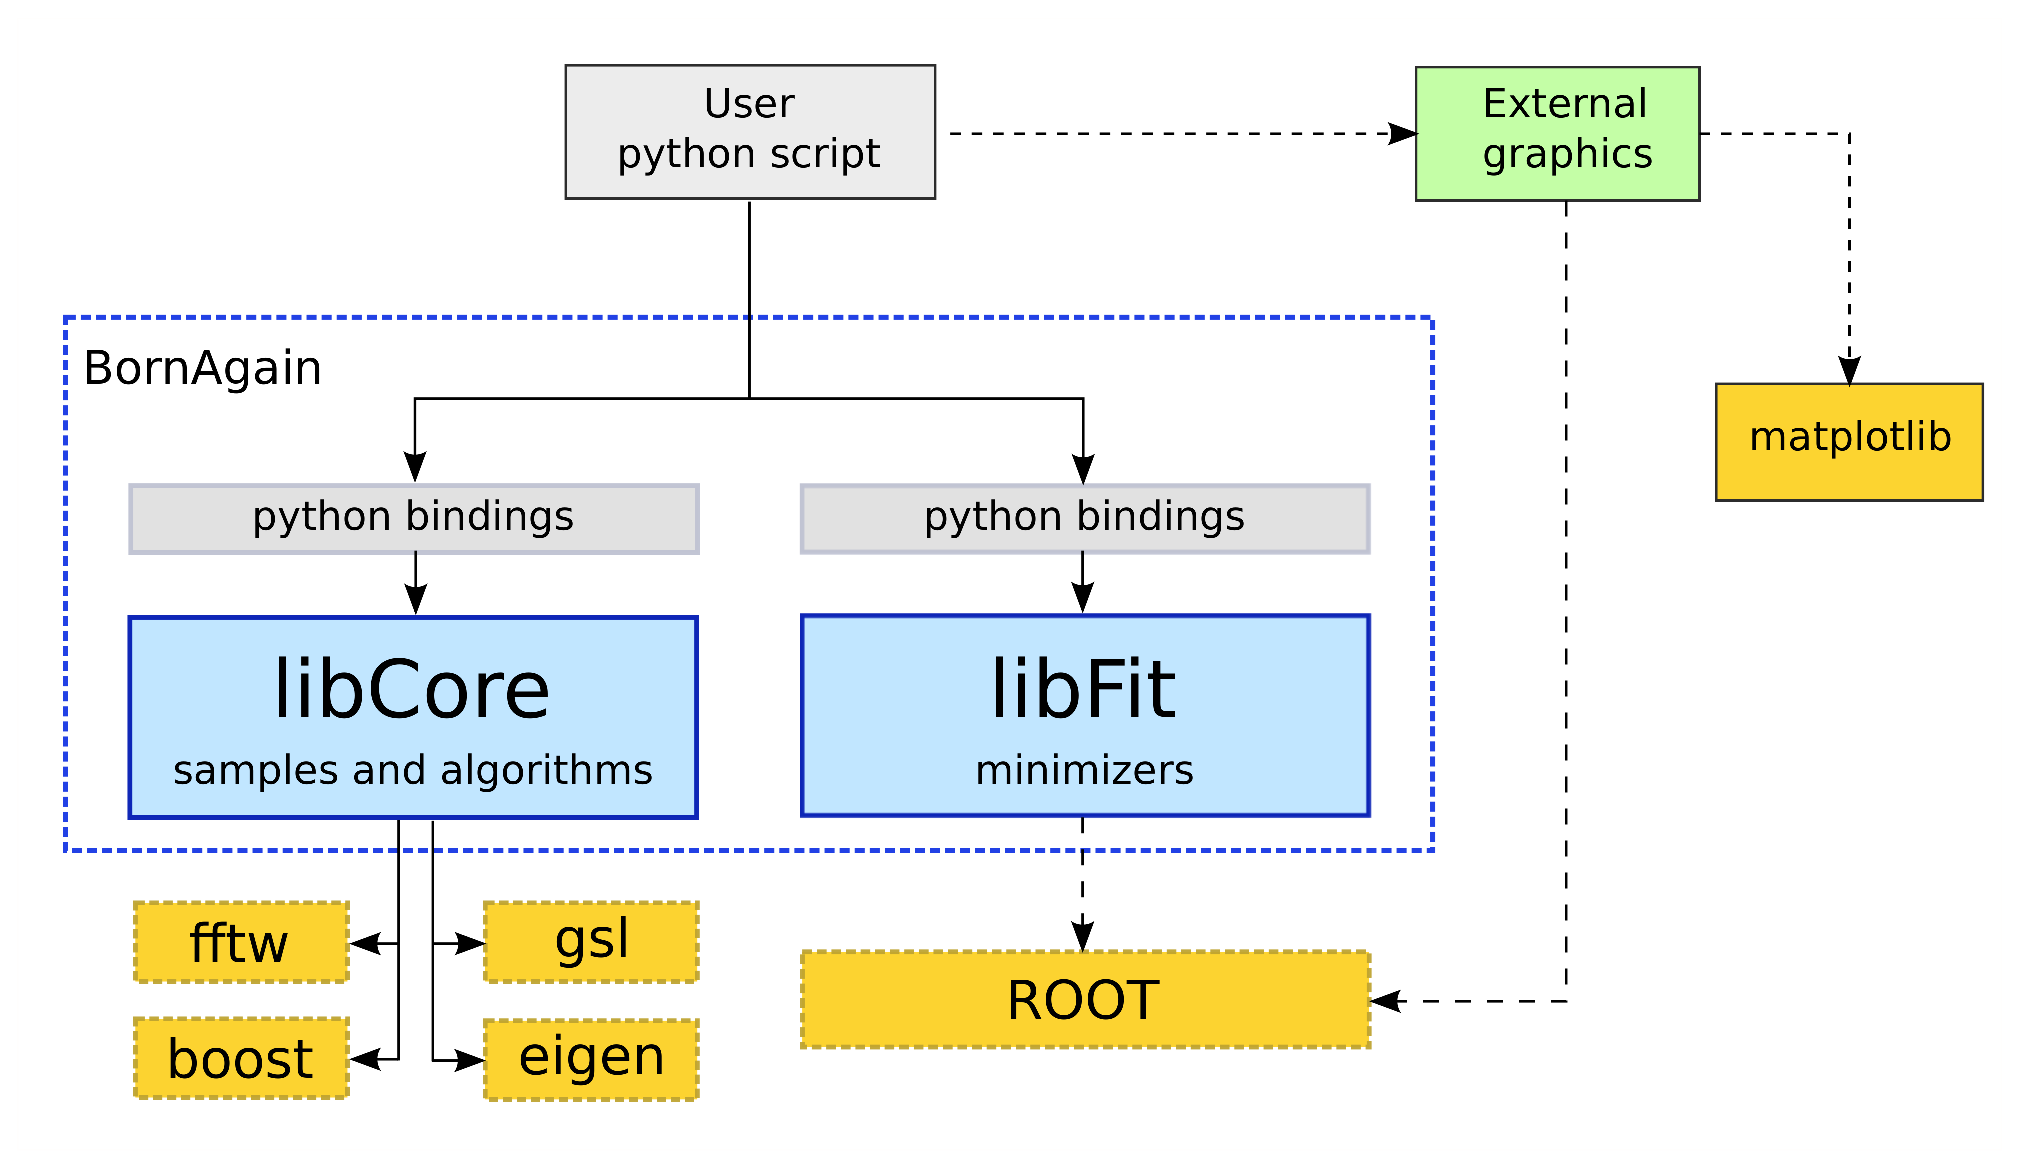
\includegraphics{fig/drawing/basic_architecture.eps}}
\caption{Structure of \BornAgain\ libraries.}
\label{fig:two_ratios}
\end{figure}


The general structure of \BornAgain\ and the way the user interacts with it are
shown in Fig.~\ref{fig:two_ratios}.
The framework consists of two shared libraries, \Code{libBornAgainCore} and
\Code{libBornAgainFit}. Thanks to the \Python\ interface they can be imported into \Python\ as external modules. The library \Code{libBornAgainCore} contains a number of classes, grouped into several class categories, necessary for the description of a model and running a simulation.
The library  \Code{libBornAgainFit} contains a number of minimization engines 
and interfaces to them, allowing the user to fit real data with the model previously defined.

\BornAgain\ depends on a few external and well established
open-source libraries: \Code{boost}, GNU scientific library, Eigen and
Fast Fourier Transformation libraries. They are required to be
installed on the system to run \BornAgain\ on Unix Platforms. In the
case of Windows Platform they are added to the system automatically during \BornAgain\ installation. Other libraries shown
on the plot (\Code{ROOT}, \Code{matplotlib}) are optional.

 
%%%%%%%%%%%%%%%%%%%%%%%%%%%%%%%%%%%%%%%%%%%%%%%%%%%%%%%%%%%%%%%%%%%%%%%%%%%%%%%%
\section{Data classes for simulations and fits}
%%%%%%%%%%%%%%%%%%%%%%%%%%%%%%%%%%%%%%%%%%%%%%%%%%%%%%%%%%%%%%%%%%%%%%%%%%%%%%%%

This section will give an overview of the classes that are used to describe all the data needed to perform a single simulation. The prime elements of this data are formed by the sample, the experimental conditions (beam and detector parameters) and simulation parameters.

These classes constitute the main interface to the software's users, since they will mostly be interacting with the program by creating samples and running simulations with specific parameters. Since it is not the intent to explain internals of classes in this document, the text and figures will only mention the most important methods and fields of the classes discussed. Furthermore, getters and setters of private member fields will not be indicated, although these do belong to the public interface. For more detailed information about the project's classes, their methods and fields, the reader is referred to the source code documentation. REF?



\subsection{The Experiment object}
The \Code{Experiment} class holds all references to data objects that are needed to perform a simulation. These consist in a sample description, possibly implemented by a builder object, detector and beam parameters and finally, a simulation parameter class that defines the different approximations that can be used during a simulation. Besides getters and setters for these fields, the class also contains a \Code{runSimulation()} method that will generate an ISimulation object that will perform the actual computations. The class diagram for \Code{Experiment} is shown in \reffig{exp}.

\vspace{8mm}
\begin{figure}[H]
%the makebox macro ensures centering of the resulting figure
\makebox[\textwidth][c]{
\begin{tikzpicture}
\begin{umlpackage}{Simulation Data}
\umlclass{Experiment}{
  -- mp\_sample : ISample* \\
  -- mp\_sample\_builder : ISampleBuilder* \\
  -- m\_detector : Detector \\
  -- m\_beam : Beam \\
  -- m\_intensity\_map : OutputData<double> \\
  -- m\_sim\_params : SimulationParameters
}{
  \umlvirt{+ clone() : Experiment*} \\
  \umlvirt{+ runSimulation() : void} \\
  \umlvirt{+ normalize() : void}
}
\umlemptyclass[x=7, y=0]{ISample}
\umlemptyclass[x=7, y=-2]{Detector}
\umlemptyclass[x=7, y=-4]{Beam}
\umlemptyclass[x=7, y=-6]{SimulationParameters}
\umlemptyclass[y=-4]{GISASExperiment}
\umluniassoc[geometry=|-, anchor1=0]{Experiment}{ISample}
\umluniassoc[geometry=|-, anchor1=0]{Experiment}{Detector}
\umluniassoc[geometry=|-, anchor1=0]{Experiment}{Beam}
\umluniassoc[geometry=|-, anchor1=0]{Experiment}{SimulationParameters}
\umlinherit[geometry=--]{GISASExperiment}{Experiment}

\umlnote[y=-6.5, width=6cm]{GISASExperiment}{
  The ``runSimulation()'' method retrieves an ISimulation object
  from the topmost ISample object and calls its ``run()'' method 
  to perform the actual computations.
}
\end{umlpackage}
\end{tikzpicture}
} %end makebox
\caption{The Experiment class as a container for sample, beam, detector and simulation parameters.}
\label{fig:exp}
\end{figure}

\subsection{The ISample class hierarchy}

Samples are described by a hierarchical tree of objects which all adhere to the ISample interface. The composite pattern is used to achieve a common interface for all objects in the sample tree. The sample description is maximally decoupled from all computational classes, with the exception of the ``createDWBASimulation()'' method. This method will create a new object of type ``DWBASimulation'' that is capable of calculating the scattering contributions originating from the sample part in question. This coupling is not very tight however, since the ISample subclasses only need to know about which class to instantiate and return.

This interface and two of its subclasses are sketched in \reffig{isample}.

\vspace{8mm}

\begin{figure}[H]
\makebox[\textwidth][c]{
\begin{tikzpicture}
\begin{umlpackage}{Sample description} 
% Code from official documentation goes here...
\umlinterface{ISample}{
}{
  \umlvirt{+ clone() : ISample*} \\
  \umlvirt{+ createDWBASimulation() : DWBASimulation*}
}
\umlclass[y=-4]{MultiLayer}{
  -- m\_layers : std::vector<Layer *> \\
  -- m\_interfaces : std::vector<LayerInterface *>
}{
  + getNumberOfLayers() : size\_t \\
  + getNumberOfInterfaces() : size\_t \\
  + addLayer(const Layer \&layer) : void
}
\umlclass[x=8,y=-4]{Layer}{
  -- mp\_material : IMaterial* \\
  -- m\_thickness : double
}{
  + getThickness() : double \\
  + setThickness(double thickness) : void
}
\umlinherit[geometry=-|]{MultiLayer}{ISample}
\umlinherit[geometry=|-]{Layer}{ISample}
\umluniassoc[geometry=--, mult2=n]{MultiLayer}{Layer}
\end{umlpackage}
\end{tikzpicture}
}
\caption{The ISample interface}
\label{fig:isample}
\end{figure}



\subsection{The FitSuite class} \SecLabel{FitSuiteClass}

\subsection{The IMinimizer class} \SecLabel{IMinimizerClass}

\subsection{The MinimizerOptions class} \SecLabel{MinimizerOptionsClass}

%\newpage{\pagestyle{empty}\cleardoublepage}


%\mychapter{1}{Appendix}

\chapter{Listings}

\begin{lstlisting}[caption={Python script of example 1},
  label=script_ex1,captionpos=b,escapeinside={@}{@} ,language=python,style=eclipse, numbers= none,frame = leftline ,
      framerule = 2mm ,
      rulecolor = \color{lightgrey},
      breaklines = true]
import sys, os, numpy 

sys.path.append(os.path.abspath(os.path.join(os.path.split(__file__)[0],'..', '..', '..', 'lib')))

from libBornAgainCore import * 

def RunSimulation():
    #  defining materials 
    mAmbience = MaterialManager.getHomogeneousMaterial("Air", 0.0, 0.0 ) 
    mSubstrate = MaterialManager.getHomogeneousMaterial("Substrate",
    6e-6, 2e-8) 
    mParticle = MaterialManager.getHomogeneousMaterial("Particle", 6e-4, 2e-8 )
    # collection of particles 
    cylinder_ff = FormFactorCylinder(5*nanometer, 5*nanometer) 
    cylinder = Particle(mParticle, cylinder_ff) 
    prism_ff = FormFactorPrism3(5*nanometer, 5*nanometer) 
    prism = Particle(mParticle, prism_ff) 
    particle_decoration = ParticleDecoration()  
    particle_decoration.addParticle(cylinder, 0.0, 0.5)  
    particle_decoration.addParticle(prism, 0.0, 0.5)  
    interference = InterferenceFunctionNone()  
    particle_decoration.addInterferenceFunction(interference)  
    # air layer with particles and substrate form multi layer 
    air_layer = Layer(mAmbience)  
    air_layer.setDecoration(particle_decoration)
    substrate_layer = Layer(mSubstrate, 0) 
    multi_layer = MultiLayer()  
    multi_layer.addLayer(air_layer) 
    multi_layer.addLayer(substrate_layer) 

    # build and run simulation  
    simulation = Simulation()  
    simulation.setDetectorParameters(100,-1.0*degree, 1.0*degree, 
                                    100, 0.0*degree, 2.0*degree, True) 
    simulation.setBeamParameters(1.0*angstrom, 0.2*degree, 0.0*degree) 
    simulation.setSample(multi_layer) 
    simulation.runSimulation()  

    # retrieving intensity data
     return GetOutputData(simulation)
\end{lstlisting}


\begin{lstlisting}[caption={Python script of fitting example},
  label=script_exfit1,captionpos=b,escapeinside={@}{@} ,language=python,style=eclipse, numbers= none,frame = leftline ,
      framerule = 2mm ,
      rulecolor = \color{lightgrey},
      breaklines = true]
import sys, os, numpy
import math 

sys.path.append(os.path.abspath(
                os.path.join(os.path.split(__file__)[0],
                '..', '..', '..', 'lib')))

from libBornAgainCore import *
from libBornAgainFit import *

# values we want to find
cylinder_height = 5.0*nanometer
cylinder_radius = 5.0*nanometer
prism3_half_side = 5.0*nanometer
prism3_height = 5.0*nanometer
# ----------------------------------
# create sample : cylinders and prisms in the air on substrate layer
# ----------------------------------
def buildSample(): 
    # defining materials
    mAmbience = MaterialManager.getHomogeneousMaterial("Air", 0.0, 0.0 )
    mSubstrate = MaterialManager.getHomogeneousMaterial("Substrate",
    6e-6, 2e-8 )
    mParticle = MaterialManager.getHomogeneousMaterial("Particle", 6e-4, 2e-8 )
    # collection of particles
    cylinder_ff = FormFactorCylinder(cylinder_height, cylinder_radius)
    cylinder = Particle(mParticle, cylinder_ff)
    prism_ff = FormFactorPrism3(prism3_height,  prism3_half_side)
    prism = Particle(mParticle, prism_ff)
    particle_decoration = ParticleDecoration()
    particle_decoration.addParticle(cylinder, 0.0, 0.5)
    particle_decoration.addParticle(prism,0.0, 0.5)  
    interference = InterferenceFunctionNone()
    particle_decoration.addInterferenceFunction(interference)
    # air layer with particles and substrate form multi layer
    air_layer = Layer(mAmbience)
    air_layer.setDecoration(particle_decoration)
    substrate_layer = Layer(mSubstrate, 0)
    multi_layer = MultiLayer()
    multi_layer.addLayer(air_layer)
    multi_layer.addLayer(substrate_layer)
    return multi_layer
# ----------------------------------
# create sample : input beam and detector - characteristics
# ----------------------------------
def createSimulation():
    simulation = Simulation()
    simulation.setDetectorParameters(100, 0.0*degree, 2.0*degree,100 , 0.0*degree, 2.0*degree)
    simulation.setBeamParameters(1.0*angstrom, 0.2*degree, 0.0*degree)
    return simulation
# ----------------------------------
# read "real" data from file
# ----------------------------------
def GetRealData():
    real_data = OutputDataIOFactory.getOutputData('Refdata_fitcylinderprisms.txt')
    return real_data
# ----------------------------------
# run fitting 
# ----------------------------------
def run_fitting():
    sample = buildSample()
    simulation = createSimulation()
    simulation.setSample(sample)
    # get the real data, which is simply results of our simulation with default values
    real_data = GetRealData()   
    # run the simulation
    simulation.runSimulation()    
    # linking real and numerical (to be fitted) data
    fitSuite = FitSuite()
    fitSuite.addSimulationAndRealData(simulation, real_data)  
    # setting fitting minimizer
    fitSuite.setMinimizer( MinimizerFactory.createMinimizer("Minuit2","Migrad") ) 
    # setting fitting parameters
    fitSuite.addFitParameter("*FormFactorCylinder/height", 4.*nanometer, 0.01*nanometer, AttLimits.lowerLimited(0.01) )
    fitSuite.addFitParameter("*FormFactorCylinder/radius", 6.*nanometer, 0.01*nanometer, AttLimits.lowerLimited(0.01) )
    fitSuite.addFitParameter("*FormFactorPrism3/height", 4.*nanometer, 0.01*nanometer, AttLimits.lowerLimited(0.01) )
    fitSuite.addFitParameter("*FormFactorPrism3/half_side", 6*nanometer, 0.01*nanometer, AttLimits.lowerLimited(0.01) )
    # run fit
    fitSuite.runFit()
    # print fit results
    fitSuite.printResults()
\end{lstlisting}


%%%%%%%%%%%%%%%%%%%%%%%%%%%%%%%%%%%%%%%%%%%%%%%%%%%%%%%%%%%%%%%%%%%%%%%%%%%%%%%%
%
%%%%%%%%%%%%%%%%%%%%%%%%%%%%%%%%%%%%%%%%%%%%%%%%%%%%%%%%%%%%%%%%%%%%%%%%%%%%%%%
\section{Gentle introduction to the data fitting.} \SecLabel{FittingGentleIntroducion}

The aim of this section is to briefly introduce the basic concept of
data fitting, its key terminology and difficulties which might arise in scattering data fit.
Users wanting to find out more about minimization (also called
maximization or optimization methods depending on the formulations and objectives) 
or looking for more rigorous discussion than provided in this manual
are referred to \cite{Antoniou2007, mntutorial}

\subsection{Toy scattering experiment.}

Fig.~\ref{fig:toyfit_data},left shows scattering intensity map in arbitrary units  
as a function of (x,y) of the detector ``measured'' in toy scattering experiment.

\begin{figure}[!p]
  \centering
    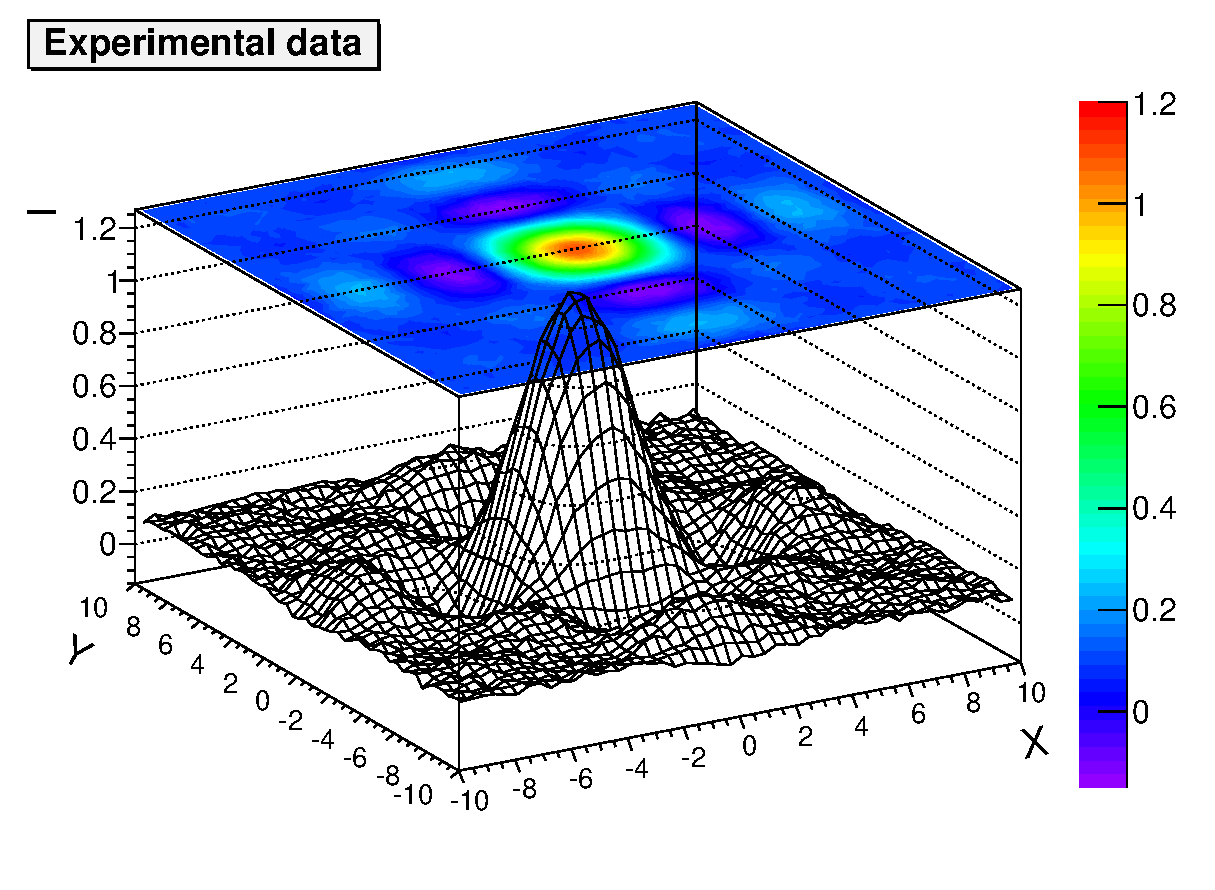
\includegraphics[width=0.49\textwidth]{Figures/toyfit_expdata.eps}
    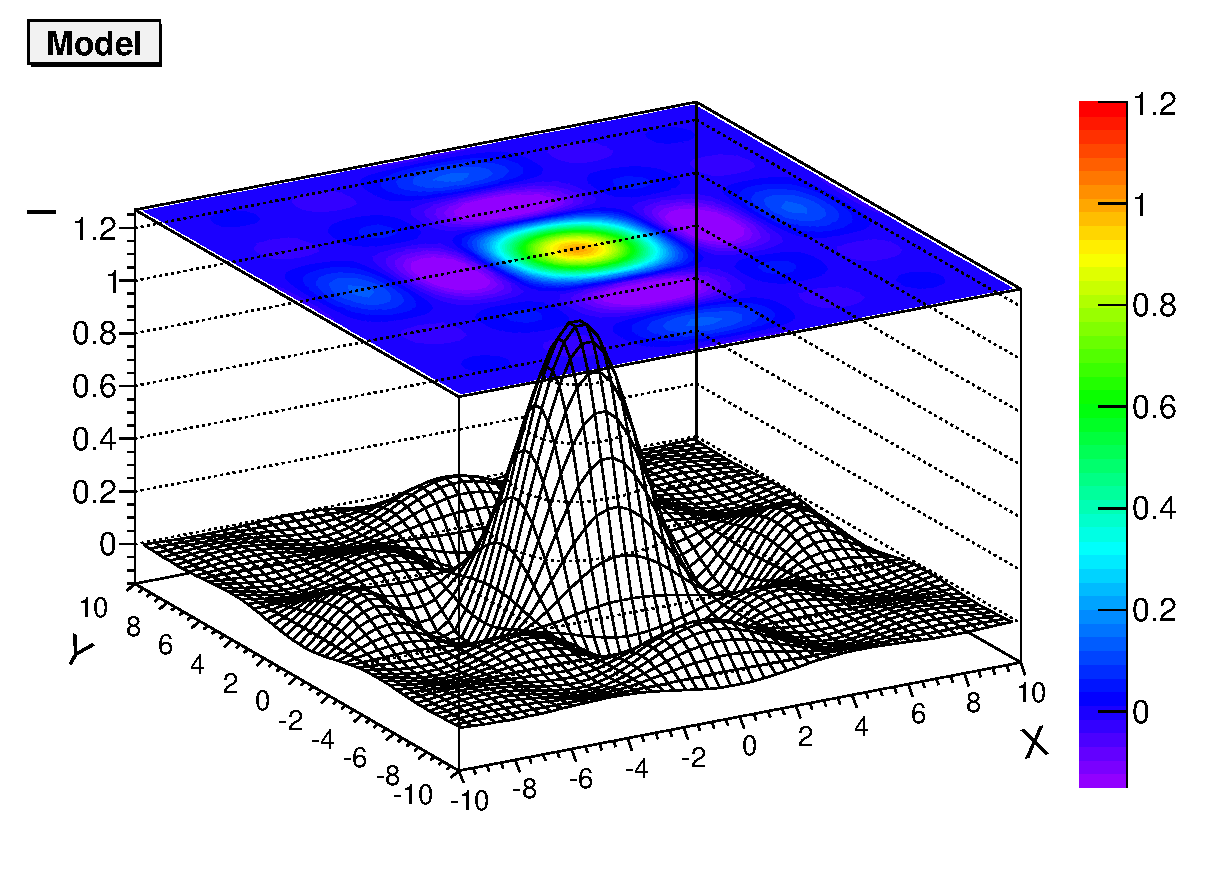
\includegraphics[width=0.49\textwidth]{Figures/toyfit_simdata.eps}
  \caption{Intensity as a function of (x,y) detector coordinates  obtained from 
  toy experiment (left) and from the toy simulation (right).   }
  \label{fig:toyfit_data}
  \vspace*{4mm}
    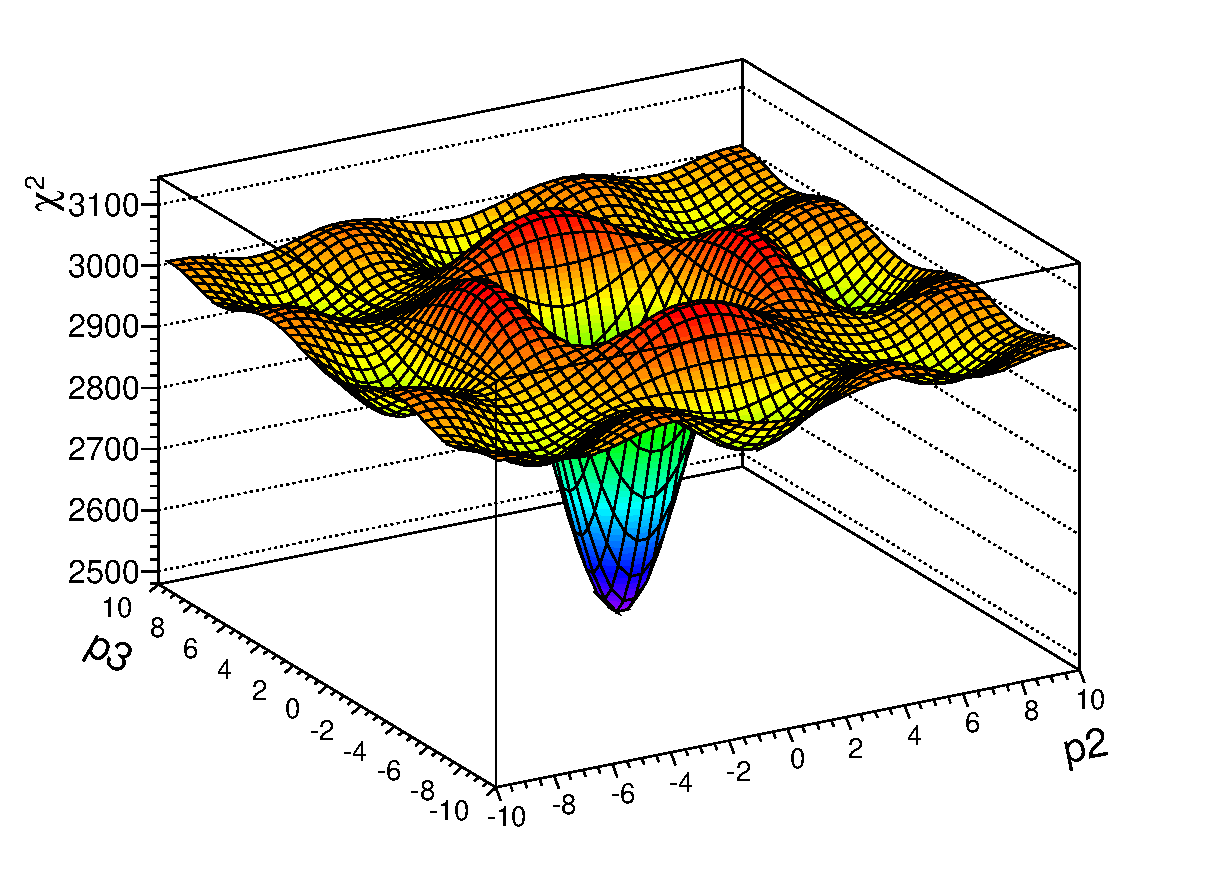
\includegraphics[width=0.49\textwidth]{Figures/toyfit_chi2_p23.eps}
    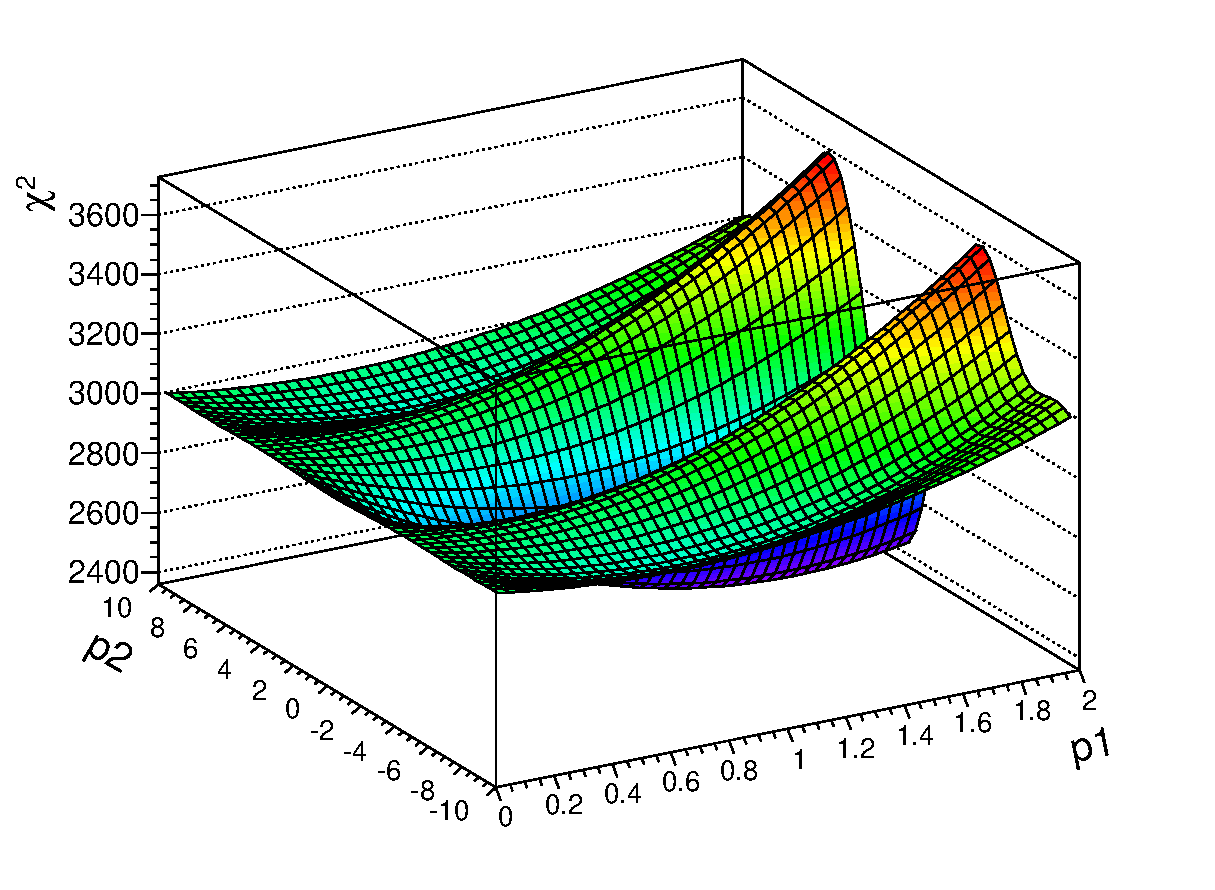
\includegraphics[width=0.49\textwidth]{Figures/toyfit_chi2_p12.eps}
  \caption{$\chi^{2}$ value calculated between experimental and simulated data
  as a function of $p_2,p_3$ parameters (left) or $p_1,p_2$ 
  parameters (right) used in the model.   }
  \label{fig:toyfit_chi2}
\end{figure}


Scattering picture presented reminds some of GISAS patterns, nevertheless it is
generated using simple function
$$I(x,y) = G(0.1,~0.01) + \frac{sin(x)}{x} \cdot \frac{sin(y)}{y}$$
Here $G(0.1, 0.01)$ is a random variable distributed according to the Gaussian distribution
with mean 0.1 and $\sigma=0.01$.
Constant $0.1$ symbolize our experimental background and constant $0.01$ is referred
to the detector noise. The rest of the formula represents our signal.

Lets define our model, namely specific mathematical function, to which we will fit our toy experimental data. By making an educated guess we assume that scattering intensity observed
in the experiment should be described with the help of $sinc$ function as follows
$$ I(x,y) = p_0 + p_1 \cdot  sinc(x - p_2) \cdot sinc(y - p_3) $$
The model has four parameters: $p_0$ describing background, $p_{1}$ describing signal strength
and $p_2,p_3$ responsible for the peak position.
Fig.~\ref{fig:toyfit_data},right shows the intensity as a function (x,y) calculated according
our model using fixed parameter set $p_0=0,p_1=1,p_2=0,p_3=0$. 

Two distributions look pretty much the same, however to find exact values of parameters which describe experimental data in the best way, one have to
\begin{itemize}
\item elaborate criteria for the difference between an actual data and its model
\item employ minimization procedure which will minimize that difference
\end{itemize}


\subsection{Objectives}

The goal is to obtain the best fit of an observed distribution
to a prediction by modifying a set of parameters from the
prediction. This problem can be one or multi-dimensional and also linear or
nonlinear. The quantity to minimize is often referred to as the
\textit{objective function}, whose expression depends on the
particular method, like the maximum likelihood, the $\chi^2$
minimization or the expected prediction error function. 

\begin{comment}
\subsubsection*{Maximum of likelihood.}
This is a popular method for parameters' estimations because the maximum likelihood estimators are approximately
unbiased and efficient for large data samples, under quite general
conditions.
We assume a sample  $\mathbf{x}=\{x_{1},x_{2},...,x_{n}\}$ of n independent and identically distributed
observations coming from probability density function $f(\mathbf{x}; \mathbf{p})$.
We assume $f(\mathbf{x}; \mathbf{p})$
to be known except for the parameters $\mathbf{p}=\{p_1,p_2,...,p_3\}$
The method of maximum likelihood takes the estimators to be
those values of $\mathbf{p}$ that maximize the likelihood function $\mathcal{L}$ as
$\mathcal{L}(\mathbf{\alpha})=\prod_{i=1}^N f(x_i;\mathbf{p})$.
Since it is easier to deal with a sum, we usually minimize
$-\text{ln}(\mathcal{L})$.
\end{comment}


\subsubsection*{$\chi^2$ or least squares minimization}
A simple dataset consist of $n$ data pairs 

\subsubsection*{Main features of minimization algorithm}



\subsection{Terminology.}

\noindent
{\bf Reference data} \\
Normally just experimental data or might be also simulated data
spoiled with the noise for purpose of testing of minimization algorithms.
\vspace*{1mm}

\noindent
{\bf Objective function} \\
Subject of minimization procedure.
\vspace*{1mm}

\noindent
{\bf Minimization} \\
Finding a best available values (i.e. local minimum) of some objective function. 
\vspace*{1mm}

\noindent
{\bf Number of degrees of freedom} \\
Number of data points - number of parameters in the fit.
\vspace*{1mm}

\noindent
{\bf Minimizer} \\
An algorithm which minimize objective function. 



\bibliographystyle{switch}
\bibliography{jw7}

\printindex

\end{document}
